% !TeX root = mos-en.tex

%%%%%%%%%%%%%%%%%%%%%%%%%%%%%%%%%%%%%%%%%%%%%%%%%%%%%%%%%%%%%%%%

\documentclass[11pt,a4paper]{article}

\usepackage{mathpazo}
\usepackage{microtype}
\usepackage{verbatim}
\usepackage{url}
\usepackage{subeqnarray}
\usepackage{caption,subcaption}

% TikZ package
\usepackage{tikz}
\usetikzlibrary{%
  calc,arrows.meta,shapes,%
  through,intersections,%
  decorations.pathmorphing}
\tikzset {>=Stealth}

% Display vertex not affected by tikz scale
\newcommand*{\vertex}[1]
  {\fill[shift only] (#1) circle (2.5pt)}
\newcommand*{\vertexcolor}[2]
  {\fill[shift only,#2] (#1) circle (2.5pt)}

% Layout
\textwidth=155mm
\textheight=230mm
\topmargin=0pt
\headheight=0pt
\oddsidemargin=0mm
\evensidemargin=0mm
\headsep=0pt
\parindent=0pt
\renewcommand{\baselinestretch}{1.1}
\setlength{\parskip}{0.3\baselineskip plus 1pt minus 1pt}

% Format problem with counter
\newcounter{problem}
\newenvironment{prob}[1]{
  \bigskip\bigskip\refstepcounter{problem}
  \addcontentsline{toc}{subsection}
  {\bfseries\theproblem{}.\ #1}
  \textbf{\Large\theproblem.\ #1\medskip\\}}{\bigskip}
\newcommand*{\que}[1]{\textbf{Q#1:}}

% Format solution
\newcommand*{\solution}[1]{\bigskip%
  \textbf{\large Solution #1} \medskip}
\newcommand*{\ans}[1]{\textbf{A#1:}}

% Annotate chapter headings
\newcommand*{\annotate}[1]{$\,^{#1}$}

% Displaystyle for fractions and combinations
\newcommand*{\disfrac}[2]{\displaystyle\frac{#1}{#2}}
\newcommand*{\dischoose}[2]{\displaystyle{#1 \choose #2}}

%\includeonly{}

\begin{document}

% \input prevents unnecessary page breakss

%% !TeX root = mos-en.tex

%%%%%%%%%%%%%%%%%%%%%%%%%%%%%%%%%%%%%%%%%%%%%%%%%%%%%%%%%%%%%%%%

\thispagestyle{empty}

\begin{center}
\textbf{\LARGE Mosteller's Challenging Problems in Probability}

\bigskip
\bigskip
\bigskip

\textbf{\Large Moti Ben-Ari}

\bigskip

\url{http://www.weizmann.ac.il/sci-tea/benari/}

\bigskip
\bigskip
\bigskip

Version $0.3$

\bigskip

\today

\end{center}

\vfill

\begin{center}
\copyright{} Moti Ben-Ari $2022$
 \end{center}
 
\begin{small}
This work is licensed under Attribution-ShareAlike 4.0 International. To view a copy of this license, visit \url{http://creativecommons.org/licenses/by-sa/4.0/}.

%\begin{center}\bf You are free to\end{center}
%
%\textit{Share:} copy and redistribute the material in any medium or format.
%
%\textit{Adapt:} remix, transform, and build upon the material
%for any purpose, even commercially.
%
%The licensor cannot revoke these freedoms as long as you follow the license terms.
%
%\begin{center}\bf Under the following terms\end{center}
%
%\textit{Attribution:} You must give appropriate credit, provide a link to the license, and indicate if changes were made. You may do so in any reasonable manner, but not in any way that suggests the licensor endorses you or your use.
%
%\textit{No additional restrictions:} You may not apply legal terms or technological measures that legally restrict others from doing anything the license permits.
\end{small}
\newpage

\tableofcontents

\newpage

\begin{center}
\textbf{\LARGE Introduction}
\end{center}

\addcontentsline{toc}{section}{\large Introduction}

\bigskip

\textbf{Frederick Mosteller}

Frederick Mosteller ($1916$--$2006$) founded the Department of Statistics at Harvard University and served as its chairman from $1957$ until $1971$, retiring from the university in $2003$. Mosteller was deeply interested in statistics education and wrote pioneering textbooks including \cite{pwsa} which emphasized the probabilistic approach to statistics, and \cite{bsda} which was one of the first texts on data analysis. In an interview Mosteller described the development of his approach to statistics education \cite{gse}.

\medskip

\textbf{This document}

This document is a ``reworking'' of Mosteller's delightful book \textit{Fifty Challenging Problems in Probability with Solutions} \cite{fifty}. The problems and their solutions are presented as far as possible in a manner accessible to readers with an elementary knowledge of probability, and many of the problems are accessible to secondary-school students and teachers. The problems and solutions have been rewritten to include detailed calculations and additional explanations and diagrams. I have sometimes included additional solutions.

Many of the problems have been modified to make them accessible: they are simplified, divided into subproblems and hints are provided. As a personal preference I have rephrased the problems in a more abstract way than Mosteller does and I have not given units like inches or currencies like dollars.

The numbering and titles of the problems have been retained to facilitate comparison with Mosteller's book.

Modern scientific calculators, including applications for smartphones, can perform the computations with no difficultly, although we use Stirling's approximation in two problems so that readers can see how it is used.

Basic concepts of probability are reviewed in the final section which is based on \cite{ross}. Since students may not be familiar with random variables and expectation, those concepts are presented in more detail.

Problems that are more difficult are annotated with $D$. Even a problem not marked $D$ can be difficult so do not be discouraged if you cannot solve it. However, it is worthwhile attempting to solve all the problems because any progress you make will be encouraging.

\textbf{Acknowledgments}

David Fortus, Aaron Montgomery, Michael Woltermann

\bigskip
\bigskip

\begin{center}
\textbf{\LARGE Simulations}
\end{center}

\addcontentsline{toc}{section}{\large Simulations}

\bigskip

\emph{Monte Carlo simulations} (named after the famous casino in Monaco) written in the Python 3 programming language are provided for most problems. A computer program ``performs an experiment,'' such as ``tossing a pair of dice'' or ``flipping a coin,'' a very large number of times and computes averages which are displayed. The random number generators built into Python, \verb+random.random()+ and \verb+random.randint()+, are used to obtain random outcomes for each experiment.

The programs run each simulation $10000$ times and the results are displayed to four decimal places. A simulated result will almost certainly not be exactly the same as that obtained from computing the expectation or the probability.

Python source code is available at \url{https://github.com/motib/probability-mosteller}. The files are named \verb+N-name.py+ where \verb+N+ is the problem number and \verb+name+ is the problem title.

For each simulation two results are displayed: 
\begin{itemize}
\item The theoretical value which is either a \emph{probability} or an \emph{expectation}. In general, rather than copy the values from the text they are calculated from the formulas. 
\item The result of the simulation is either a \emph{proportion} of successes relative to the number of trials corresponding to a probability, or the \emph{average} number of successes corresponding to an expectation.
\end{itemize}
It is important to understand that ``probability'' and ``expectation'' are theoretical concepts. The \emph{law of large numbers} ensures that the outcomes of many trials are very close to the theoretical values, but they won't be exactly the same. For example, the probability of obtaining a $6$ when a fair die is thrown is $1/6\approx 0.1667$. Running a simulation for $10000$ throws resulted in a range of values: $0.1684, 0.1693, 0.1687, 0.1665, 0.1656$.

The simulation programs are very short and straightforward once a problem is understood. I suggest running the simulations for various numbers of trials and other parameters to help understand their sensitivity to these parameters.

. You can run the program many times to see how the results vary
%% !TeX root = mos-en.tex

%%%%%%%%%%%%%%%%%%%%%%%%%%%%%%%%%%%%%%%%%%%%%%%%%%%%%%%%%%%%%

\begin{center}
\textbf{\LARGE Problems and solutions}
\end{center}

\addcontentsline{toc}{section}{\large Problems and solutions}

\begin{prob}{The sock drawer}
A drawer contains red and black socks. If two socks are drawn at random without replacement the probability that both are red is $\frac{1}{2}$. 

\que{1} How small can the number of black socks in the drawer be? What is the corresponding number of red socks?

\que{2} How small can the number of black socks in the drawer be if the number of black socks is \emph{even}? What is the corresponding number of red socks?
\end{prob}

\solution{1}

\ans{1} Let $r$ be the number of red socks in the drawer and let $b$ the number of black socks.  $r\geq 2$ since two red socks are drawn and $b\geq 1$ since otherwise the probability of drawing two red socks would be $1$.

Multiplying the probabilities for the two draws gives:
\begin{equation}\label{eq.1-a}
P(\textsf{two red})=\frac{r}{r+b} \cdot \frac{(r-1)}{(r-1)+b} = \frac{1}{2}\,.
\end{equation}
Simplifying results in a quadratic equation in the variable $r$:
\begin{equation}\label{eq.quad-for-r}
r^2-r(2b+1)-(b^2-b)=0\,.
\end{equation}
Since $r,b$ are positive integers the discriminant must be the square of an integer:
\begin{equation}\label{eq.discriminant}
(2b+1)^2+4(b^2-b)=8b^2+1
\end{equation}
The discriminant is a square when $b=1$ (its smallest value). From Equation~\ref{eq.quad-for-r}, $r=3$ where we reject the solution $r=0$ because $r\geq 2$. The total number of socks is $4$.

Check: $\frac{3}{4}\cdot\frac{2}{3}=\frac{1}{2}$.

\medskip

\ans{2}
Check positive even values of $b$ to find the smallest one for which the discriminant is a square:
\begin{displaymath}
\renewcommand{\arraystretch}{1}
\begin{array}{r|r|r}
b&8b^2+1&\sqrt{8b^2+1}\\
\hline
2&33&5.74\\
4&129&11.36\\
\mathbf{6}&\mathbf{289}&\mathbf{17}
\end{array}
\end{displaymath}
For $b=6$ the corresponding value for $r$ is $15$.

Check: $\frac{15}{21}\cdot\frac{14}{20}=\frac{1}{2}$.

\newpage

\solution{2}

\ans{1}
Is the following inequality is true?
\begin{equation}\label{eq.1-b}
\frac{r}{r+b} \stackrel{?}{>} \frac{r-1}{(r-1)+b}\,.
\end{equation}
$r\geq 2, b\geq 1$, so both denominators are positive and we can multiply the two sides:
\begin{eqn}
r(r-1+b)&\stackrel{?}{>}&(r-1)(r+b)\\
r^2-r+rb&\stackrel{?}{>}&r^2-r+rb-b\\
b&\stackrel{?}{>}&0\,.
\end{eqn}%
$b>1$ so Equation~\ref{eq.1-b} is true.

By Equations~\ref{eq.1-a}, \ref{eq.1-b}:
\begin{equation}\label{eq.1-c}
\left(\frac{r}{r+b}\right)^2 = \frac{r}{r+b} \cdot\frac{r}{r+b} > \frac{r}{r+b} \cdot \frac{r-1}{(r-1)+b} = \frac{1}{2}\,,
\end{equation}
and similarly:
\begin{equation}\label{eq.1-d}
\left(\frac{r-1}{(r-1)+b}\right)^2  = \frac{r-1}{(r-1)+b}\cdot \frac{r-1}{(r-1)+b}<  \frac{r}{r+b} \cdot \frac{r-1}{(r-1)+b} = \frac{1}{2}\,.
\end{equation}
$r+b$ is non-zero so we can take the square root of Equation~\ref{eq.1-c} and simplify:
\begin{eqn}
\frac{r}{r+b}  &>& \sqrt{\frac{1}{2}}\\
r&>&\frac{b}{\sqrt{2}-1}=\frac{b}{\sqrt{2}-1}\cdot\frac{\sqrt{2}+1}{\sqrt{2}+1}\\
r&>&b(\sqrt{2}+1)\,.
\end{eqn}%
Similarly for Equation~\ref{eq.1-d}:
\begin{eqn}
\frac{r-1}{(r-1)+b}&<&\sqrt{\frac{1}{2}}\\
r-1 &<& \frac{b}{\sqrt{2}-1}\\
r-1&<&b(\sqrt{2}+1)\,.
\end{eqn}%
Combining both equations we get:
\begin{equation}\label{eq.inequalities}
r-1<(\sqrt{2}+1)b<r\,.
\end{equation}
For $b=1$ we have $2.141 < r< 3.141$ and $b=1,r=3$ is a solution.

\ans{2} Check positive even values of $b$:
\begin{displaymath}	
\renewcommand{\arraystretch}{1}
\begin{array}{r|ccc|c|c}
b& (\sqrt{2}+1)b&<r<& (\sqrt{2}+1)b+1&r&P(\textrm{two reds})\\
\hline
2&4.8&<r<&5.8&5&0.4762\\
4&9.7&<r<&10.7&10&0.4945\\
6&14.5&<r<&15.5&
15&0.5000
\end{array}
\end{displaymath}
Mosteller mentions a connection between this problem and advanced number theory, and gives another solution: $b=35,r=85$.

\medskip
\textbf{Simulation}
\begin{verbatim}
Expectation of both red  = 0.5000
Average of both red for (red =  3, black =  1) = 0.5053
Average of both red for (red = 15, black =  6) = 0.5013
Average of both red for (red = 85, black = 35) = 0.4961
\end{verbatim}

\textbf{Comment}

Neither solution provides a \emph{sufficient} condition for the values of $r,b$. In Solution~1 we derive a necessary condition---by Equation~\ref{eq.discriminant} the discriminant must be an integer---and start searching for values of $b$ that satisfy this requirement. In Solution~2 the necessary condition is that $r,b$ must satisfy the inequalities in Equation~\ref{eq.inequalities} and then we search for values that satisfy the requirement that the probability of two reds must be $0.5$.

I wrote a program to search for solutions. For $r$ near $35$:
\[
\renewcommand{\arraycolsep}{12pt}
\begin{array}{r|r|r|r}
\multicolumn{1}{c|}{r}&
\multicolumn{1}{c|}{b}&
\multicolumn{1}{c|}{\sqrt{8b^2+1}}&
\multicolumn{1}{c}{P(\textsf{two red})} \\\hline
32 & 78  & 90.52 & 0.500917\\
33 & 80  & 93.34 & 0.499368\\
34 & 83  & 96.17 & 0.501474\\
35 & 85  & 99.00 & 0.500000\\
36 & 87  &101.83 & 0.498601\\
37 & 90  &104.66 & 0.500562
\end{array}
\]
Here are the solutions for $b<10^6$:
\[
\begin{array}{r@{\hspace{2em}}r}
\textsf{black} & \textsf{red}\\\hline
1 & 3 \\
6 & 15\\
35 &  85\\
204 &  493\\
1189 &  2871\\
6930 & 16731\\
40391 &  97513\\
235416 & 568345
\end{array}
\]

%%%%%%%%%%%%%%%%%%%%%%%%%%%%%%%%%%%%%%%%%%%%%%%%%%%%%%%%%%%%%

\begin{prob}{Successive wins}
You play a sequence of three games alternately against two players and you win the sequence if you win at least two of the three games \emph{in a row}. The probability that you will win a game against player $P_1$ is $p_1$ and the probability that you will win a game against player $P_2$ is $p_2$. It is given that $p_1>p2$. Which of these sequences gives you a better chance of winning?
\begin{itemize}
\item You play against $P_1,P_2,P_1$ in that order.
\item You play against $P_2,P_1,P_2$ in that order.
\end{itemize}
\end{prob}

\solution{1}

You win if: (a) you win the first two games and lose the last game, (b) you lose the first game and win the last two games, or (c) you win all three games.

Let $p_{121}$ be the probability that you win with the sequence $P_1,P_2,P_1$ and let $p_{212}$ be the probability that you win with the sequence $P_1,P_1,P_2$. Then:
\begin{eqn}
p_{121}&=&p_1p_2(1-p_1) + (1-p_1)p_2p_1 + p_1p_2p_1\\
p_{212}&=&p_2p_1(1-p_2) + (1-p_2)p_1p_2 + p_2p_1p_2\,.
\end{eqn}%
You have a better chance of winning with the sequence $P_1,P_2,P_1$ if $p_{121}>p_{212}$, that is, if:
\[
p_1p_2(1-p_1) + (1-p_1)p_2p_1 + p_1p_2p_1 \stackrel{?}{>} 
p_2p_1(1-p_2) + (1-p_2)p_1p_2 + p_2p_1p_2\,.
\]
Cancel $p_1p_2$ from all terms:
\begin{eqn}
(1-p_1)+(1-p_1)+p_1 & \stackrel{?}{>}& (1-p_2)+(1-p_2)+p_2\\
-p_1&\stackrel{?}{>}&-p_2\\
p_2&\stackrel{?}{>}&p_1\,,
\end{eqn}%
but by assumption $p_1>p_2$ so you should choose the sequence $P_2,P_1,P_2$,

\solution{2}

The result is counter-intuitive. Intuitively, you should choose to play two games with $P_1$ and one game with $P_2$ because more likely to win games against $P_1$. However, the only way that you can win the sequence is by winning the \emph{middle} game, and, therefore, you should play the middle game against $P_1$, the player you are more likely to defeat.

\newpage

\textbf{Simulation}
\begin{verbatim}
For p1 = 0.6, p2 = 0.5
Proportion of P121 wins = 0.4166
Proportion of P212 wins = 0.4473

For p1 = 0.6, p2 = 0.4
Proportion of P121 wins = 0.3300
Proportion of P212 wins = 0.3869

For p1 = 0.6, p2 = 0.2
Proportion of P121 wins = 0.1625
Proportion of P212 wins = 0.2141
\end{verbatim}

%%%%%%%%%%%%%%%%%%%%%%%%%%%%%%%%%%%%%%%%%%%%%%%%%%%%%%%%%%%%%

\begin{prob}{The flippant juror}
There are two options to reach a decision: (a) A three-person panel consisting of two members who independently make the correct decision with probability $p$ and one member who makes the correct decision with probability $1/2$. The final decision is determined by a majority vote. (b) A one-person panel whose only member has probability $p$ of making the correct decision. Which option has the higher probability of making the correct decision?
\end{prob}

\solution{}

The three-person panel makes the correct decision if all three members make the correct decision or if any subset of two members makes the correct decision:
\[
P(\textsf{correct decision})=\overbrace{\left(p\cdot p\cdot\frac{1}{2}\right)}^{\textsf{all three correct}}+\;\;\overbrace{\left(p(1-p)\cdot\frac{1}{2}+(1-p)p\cdot\frac{1}{2}+p\cdot p\cdot\frac{1}{2}\right)}^{\textsf{two out of three correct}}=p\,,
\]
so there is no difference between the two options.

\textbf{Simulation}
\begin{verbatim}
Prediction: probabilities of (a) and (b) are equal
For p = 0.25, proportion correct of (a) = 0.5019, (b) = 0.5046
For p = 0.50, proportion correct of (a) = 0.5072, (b) = 0.4970
For p = 0.75, proportion correct of (a) = 0.5062, (b) = 0.5040
\end{verbatim}

%%%%%%%%%%%%%%%%%%%%%%%%%%%%%%%%%%%%%%%%%%%%%%%%%%%%%%%%%%%%%

\newpage

\begin{prob}{Trials until first success}
\label{p.four}
What is the expectation of the number of throws of a die until a $6$ appears?
\end{prob}

\solution{1}

The probability that the $i$th throw will be the first occurrence of $6$ is the probability of $i-1$ throws of one of the other five numbers times the probability that the $i$th throw will be $6$.

To simplify notation let $p=1/6$, $P=P(\textsf{first}\:6\:\textsf{on}\:i\textsf{th throw})$, $E=E(\textsf{first throw of}\:6)$. Then:
\begin{eqnlabels}
\nonumber{}P&=&(1-p)^{i-1}p\\
\label{eq.first-expec}E&=&1p(1-p)^0 + 2p(1-p)^1+ 3p(1-p)^2+ 4p(1-p)^3 +\cdots =\sum_{i=1}^{\infty} ip(1-p)^{i-1}\,.
\end{eqnlabels}
Without the factor $i$ the sum would be the probability of eventually throwing a $6$:
\begin{equation}\label{eq.geo}
P(\textsf{eventually throwing a}\;6)= \sum_{i=1}^{\infty} p(1-p)^{i-1}=p\cdot\frac{1}{1-(1-p)}=1\,,
\end{equation}
which is not a surprising result.

The calculation of the expectation can be performed as follows:
\[
\renewcommand{\arraycolsep}{2pt}
\begin{array}{lllllllllll}
E&\!\!=\!\!&p(1-p)^0 &+& p(1-p)^1&+& p(1-p)^2&+& p(1-p)^3 &+&\cdots \\
& & &&p(1-p)^1&+& p(1-p)^2&+& p(1-p)^3 &+&\cdots \\
&  &&&& &p(1-p)^2&+& p(1-p)^3 &+&\cdots \\
&&&&&&&&p(1-p)^3 &+&\cdots
\end{array}
\]
The first row is the sum of the geometric series from Equation~\ref{eq.geo} which is $1$. The second row is the same geometric series except that the first element is $p(1-p)$ so its sum is:
\[
\frac{p(1-p)}{1-(1-p)}=1-p\,.
\]
Similarly, the sum of the third row will be $(1-p)^2$ and the sum of the $i$th row will be $(1-p)^{i-1}$. Therefore, the expectation is the sum of the geometric series:
\[
E= 1 + (1-p) + (1-p)^2 + (1-p)^3 + \cdots= \frac{1}{1-(1-p)}=\frac{1}{p}=6\,.
\]

\solution{2}

Multiply Equation~\ref{eq.first-expec} by $1-p$ and subtract the result from that equation. The result is the geometric series in Equation~\ref{eq.geo}:
\[
\renewcommand{\arraycolsep}{2pt}
\begin{array}{rclllllllll}
E&=&p(1-p)^0 &+&2p(1-p)^1&+& 3p(1-p)^2&+& 4p(1-p)^3 &+&\cdots\\
E\cdot(1-p)&=&&&p(1-p)^1 &+& 2p(1-p)^2&+& 3p(1-p)^3 &+&\cdots \\
E\cdot(1-(1-p)) &=& p &+& p(1-p)^1 &+& p(1-p)^2 &+& p(1-p)^3 &+&\cdots\\
Ep&=&1\\
E&=&1/p=6\,.
\end{array}
\]

\solution{3}

Consider the first throw separately from the rest of the throws. If the first throw is a $6$ (probability $p$) then one throw is sufficient. Otherwise, if the first throw is not a $6$ (probability $1-p$), then the remaining throws form a sequence identical to the original one so the expectation of this sequence is $E$:
\begin{eqn}
E &=& 1p + (E+1)(1-p)\\
E&=&1/p=6\,.
\end{eqn}%

\textbf{Simulation}
\begin{verbatim}
Expectation of first success = 6
Average of first success     = 6.0161
\end{verbatim}

%%%%%%%%%%%%%%%%%%%%%%%%%%%%%%%%%%%%%%%%%%%%%%%%%%%%%%%%%%%%%


\begin{prob}{Coin in a square}

A coin is thrown onto an (unbounded) grid of squares of uniform size. The position of the center of the coin is uniformly distributed within the square in which it lands.

\que{1} Given a square of side $8$ and a coin of radius $3$ what is the probability that the coin lands entirely within the square?

\que{2} For each throw you win $5$ if the coin lands within the square and lose $1$ if it touches a side of the square. What is the expectation of your winnings for each throw?

\que{3} Develop a formula for the probability of the coin landing within the square if the side of the square is $a$ and the radius of the coin is $r<a/4$.
\end{prob}

\solution{}

\ans{1} \ref{f.coins1} shows a square of side $8$ and four circles of radius $3$ inscribed within the corners of the square. The centers of the circles form an inner square of side $2$. Any coin whose center is outside the inner square will touch an edge of the outer square. Since the center of the coin is uniformly distributed, the probability that the coin lands entirely within the square is the ratio of the area of the inner square to the area of the outer square:
\[
P(\textsf{coin lands within the square})=\frac{2\cdot 2}{8\cdot 8} =\frac{1}{16}=0.0625\,.
\]
\begin{figure}[tb]
\begin{center}
\begin{subfigure}{.43\textwidth}
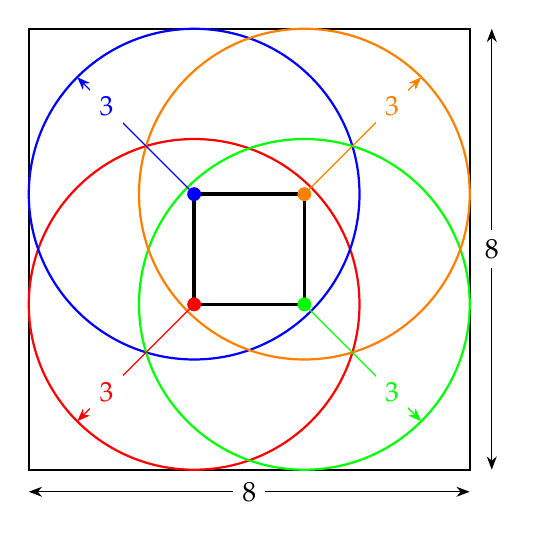
\begin{tikzpicture}[scale=.7]
\coordinate (c1) at (3,3);
\coordinate (c2) at (3,5);
\coordinate (c3) at (5,3);
\coordinate (c4) at (5,5);
\draw[very thick] (c1) -- (c3) -- (c4) -- (c2) -- cycle;
\draw[thick] (0,0) rectangle +(8,8);
\draw[color=red,thick] (c1) circle[radius=3];
\draw[color=blue,thick] (c2) circle[radius=3];
\draw[color=green,thick] (c3) circle[radius=3];
\draw[color=orange,thick] (c4) circle[radius=3];
\vertexcolor{c1}{red};
\vertexcolor{c2}{blue};
\vertexcolor{c3}{green};
\vertexcolor{c4}{orange};
\draw[<->] (0,-.4) -- node[fill=white] {$8$} (8,-.4);
\draw[<->] (8.4,0) -- node[fill=white] {$8$} (8.4,8);
\draw[->,red] (3,3) -- node[near end,fill=white] {$3$} +(-135:3);
\draw[->,blue] (3,5) -- node[near end,fill=white] {$3$} +(135:3);
\draw[->,green] (5,3) -- node[near end,fill=white] {$3$} +(-45:3);
\draw[->,orange] (5,5) -- node[near end,fill=white] {$3$} +(45:3);
\end{tikzpicture}
\caption{Coins contained in the square}\label{f.coins1}
\end{subfigure}
\hspace{3em}
\begin{subfigure}[b]{.43\textwidth}
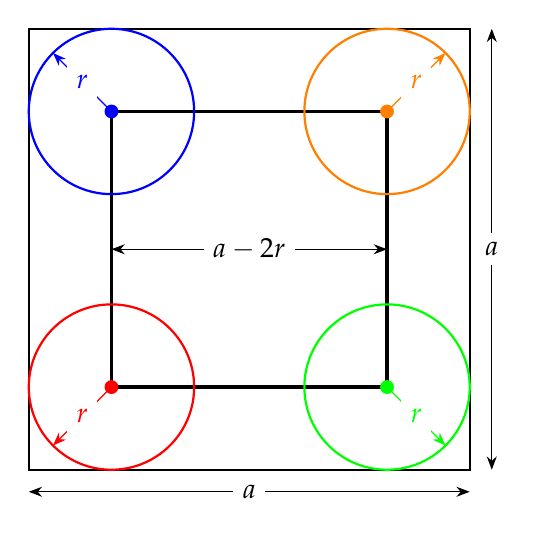
\begin{tikzpicture}[scale=.7]
\coordinate (c1) at (1.5,1.5);
\coordinate (c2) at (1.5,6.5);
\coordinate (c3) at (6.5,1.5);
\coordinate (c4) at (6.5,6.5);
\draw[very thick] (c1) -- (c3) -- (c4) -- (c2) -- cycle;
\draw[thick] (0,0) rectangle +(8,8);
\draw[color=red,thick] (c1) circle[radius=1.5];
\draw[color=blue,thick] (c2) circle[radius=1.5];
\draw[color=green,thick] (c3) circle[radius=1.5];
\draw[color=orange,thick] (c4) circle[radius=1.5];
\vertexcolor{c1}{red};
\vertexcolor{c2}{blue};
\vertexcolor{c3}{green};
\vertexcolor{c4}{orange};
\draw[<->] (0,-.4) -- node[fill=white] {$a$} (8,-.4);
\draw[<->] (8.4,0) -- node[fill=white] {$a$} (8.4,8);
\draw[->,red] (1.5,1.5) -- node[fill=white] {$r$} +(-135:1.5);
\draw[->,blue] (1.5,6.5) -- node[fill=white] {$r$} +(135:1.5);
\draw[->,green] (6.5,1.5) -- node[fill=white] {$r$} +(-45:1.5);
\draw[->,orange] (6.5,6.5) -- node[fill=white] {$r$} +(45:1.5);
\draw[<->] (1.5,4) -- node[fill=white] {$a-2r$} (6.5,4);
\end{tikzpicture}
\caption{Coins in a large square}\label{f.coins2}
\end{subfigure}
\end{center}
\end{figure}

\ans{2}
\[
E(\textsf{winnings per throw})=5\cdot\frac{1}{16}\,+\,(-1)\cdot\frac{15}{16}=-\frac{10}{16}=-0.625\,.
\]

\ans{3} \ref{f.coins2} shows four circles inscribed in the corners of the square. The side of the inner square is $a-2r$ so:
\[
P(\textsf{coin lands within the square})=\frac{(a-2r)^2}{a^2}\,.
\]
\textbf{Simulation}
\begin{verbatim}
For side = 8, radius = 1:
Probability of landing within the square = 0.5625
Proportion landing within the square     = 0.5704
For side = 8, radius = 2:
Probability of landing within the square = 0.2500
Proportion landing within the square     = 0.2481
For side = 8, radius = 3:
Probability of landing within the square = 0.0625
Proportion landing within the square     = 0.0639
For side = 8, radius = 4:
Probability of landing within the square = 0.0000
Proportion landing within the square     = 0.0000
\end{verbatim}

%%%%%%%%%%%%%%%%%%%%%%%%%%%%%%%%%%%%%%%%%%%%%%%%%%%%%%%%%%%%%

\begin{prob}{Chuck-a-luck}
Choose number $n$ between $1$ and $6$ and throw three dice. If $n$ does not appear on any of the dice you lose $1$; if $n$ appears on one die you win $1$; if $n$ appears on two dice you win $2$; if $n$ appears on three dice you win $3$. What is the expectation of your winnings?
\end{prob}

\newpage

\solution{}

Let $P(k)$ be the probability that $n$ appears on $k$ dice. Then:
\[
E(\textsf{winnings per throw})=-1 P(0) + 1 P(1) + 2 P(2) + 3 P(3)\,.
\]
The throws of the three dice are independent so:
\begin{eqn}
E(\textsf{winnings per throw}) &=& 
-1 \dischoose{3}{0}\left(\frac{1}{6}\right)^0\left(\frac{5}{6}\right)^3
+1\dischoose{3}{1}\left(\frac{1}{6}\right)^1\left(\frac{5}{6}\right)^2+\\
&&\;\;\; 2{3\choose 2}\left(\frac{1}{6}\right)^2\left(\frac{5}{6}\right)^1+
3\dischoose{3}{3}\left(\frac{1}{6}\right)^3\left(\frac{5}{6}\right)^0\\
&=& \frac{1}{216}(-125+75+30+3)\approx -0.0787\,.
\end{eqn}%

\textbf{Simulation}
\begin{verbatim}
Expectation of winnings = -0.0787
Average winnings        = -0.0724
\end{verbatim}

%%%%%%%%%%%%%%%%%%%%%%%%%%%%%%%%%%%%%%%%%%%%%%%%%%%%%%%%%%%%%

\begin{prob}{Curing the compulsive gambler}

\label{p.roulette}Roulette is a game played with a wheel having $38$ numbered pockets: $18$ red, $18$ black and $2$ green.\footnote{There are two green pockets in American roulette and one green pocket in European roulette.} The wheel is spun, a ball is thrown onto the wheel and you wait until the ball lands in one of the pockets. The ball lands in a random pocket with uniform distribution. You bet $1$ that the ball will land in a specific numbered (red or black) pocket.\footnote{This is the only type of bet used in the problems in this book.} If the ball lands in that pocket you receive $36$. Your net winnings are actually $35$ because the the $36$ includes the $1$ bet which is returned.

\que{1} What is the expectation your winnings if you play $36$ round of roulette?

\que{2} Your friend offers to bet you $20$ that after $36$ rounds you will have \emph{lost} money. What is the expectation of your winnings, taking into account the money won or lost both from the game and the bet with your friend?
\end{prob}

\solution{}

\ans{1} The probability of winning a single round is $1/38$ so:
\begin{eqn}
E(\textsf{winnings in one round})&=&35\cdot \frac{1}{38} + (-1)\cdot\frac{37}{38} = -\frac{2}{38} \approx -0.0526\\
E(\textsf{winnings in}\;36\;\textsf{rounds})&=&36\cdot -0.05266=-1.8947\,.
\end{eqn}%

\ans{2}
Consider the four outcomes of playing roulette for $36$ rounds:
\begin{itemize}
\item If you lose all the rounds you lose $36$.
\item If you win one round you win $35$ and you lose $35$ on the other rounds no money is won or lost.
\item If you win two rounds you win $70$ and you lose $34$ on the other rounds for a net win of $36$.
\item In general if you win $k$ rounds for $2<k\leq 36$ your net win is $35k - (36-k)>0$.
\end{itemize}
Therefore, you lose the bet only if you lose all rounds:
\begin{eqn}
P(\textrm{losing\ } 36 \textrm{\ rounds})&=&\left(\frac{37}{38}\right)^{36}\approx 0.3829\\
E(\textsf{total winnings})&=&\overbrace{-1.8947}^{\textsf{\small E of all rounds}}+\;\;
\overbrace{-20\cdot 0.3829}^{\textsf{\small lose bet}} \;+\; \overbrace{20\cdot (1-0.3829))}^{\textsf{\small win bet}} \approx 2.7904\,.
\end{eqn}%
Clearly you should take the bet!

\textbf{Simulation}
\begin{verbatim}
Expectation of winning a round = -0.0526
Average winnings for a round   = -0.0593
\end{verbatim}
The simulation showed a large variance which was reduced by running one million trials.

%%%%%%%%%%%%%%%%%%%%%%%%%%%%%%%%%%%%%%%%%%%%%%%%%%%%%%%%%%%%%

\begin{prob}{Perfect bridge hand}
Randomly select $13$ cards from a deck. What is the probability that they will all be of the same suit?
\end{prob}

\solution{1}

There are $\dischoose{52}{13}$ ways of selecting $13$ cards from a deck of $52$ cards. Only four of them consist of $13$ cards from the same suit:
\[
P(\textsf{selecting}\;13\;\textsf{of same suit})=\frac{4}{\dischoose{52}{13}}=\frac{4\cdot 13!\cdot 39!}{52!}\approx 6.2991\times 10^{-12}\,.
\]

\solution{2}

There are $52$ ways of selecting the first card, then $12$ ways of selecting the second card of the same suit from the remaining $51$ cards, $11$ ways of selecting a third card, and so on:
\[
P(\textsf{selecting}\;13\;\textsf{cards of the same suit})=\frac{52}{52}\cdot \frac{12}{51}\cdot \frac{11}{50} \cdots  \frac{1}{40}= \frac{12!}{51!/39!}\approx 6.2991\times 10^{-12}\,.
\]

\newpage

\textbf{Simulation}

There is no point in running a simulation with $52$ cards because the result would almost certainly be zero. A simulation was run with a deck of $16$ cards and $4$ suits.

\begin{verbatim}
Probability of perfect hand = 0.0022
Proportion perfect hand     = 0.0020
\end{verbatim}

%%%%%%%%%%%%%%%%%%%%%%%%%%%%%%%%%%%%%%%%%%%%%%%%%%%%%%%%%%%%%

\begin{prob}{Craps\annotate{D}}
Craps is a played with a pair of dice. On the first throw you win if the sum of the numbers is $7$ or $11$ and you lose if the sum is $2$, $3$ or $12$. If the sum on the first throw is $n=4,5,6,8,9,10$ (called a \emph{point}), continue to throw the dice until the sum is the point $n$ (a win) or $7$ (a loss).

\que{1} What are the probabilities of the following events on the first throw: winning, losing, neither winning nor losing?

\que{2} What is the probability of a win?
\end{prob}

\solution{1}

\ans{1} The outcome of throwing a die is uniformly distributed and the outcomes of throwing a pair of dice are independent, so the probability of any outcome is $1/36$. The number of ways of obtaining each of the events, the sum of a pair of dice, is:
\[
\begin{array}{l|rrrrrrrrrrr}
\textrm{Sum} & 2 & 3 & 4 & 5 & 6 & 7 & 8 & 9 & 10 & 11 & 12\\\hline
\textrm{Pairs} & 1 & 2 & 3 & 4 & 5 & 6 & 5 & 4 & 3 & 2 & 1
\end{array}
\]
On the first throw there are $8$ ways of throwing $7$ or $11$ so the probability of winning is $8/36$ and there are $4$ ways of throwing $2,3,12$ so the probability losing is $4/36$. The probability of neither winning nor losing on the first throw is:
\[
1 - \frac{8}{36} - \frac{4}{36} = \frac{24}{36}\,.
\]

%%%%%%%%%%%%%%%%%%%%%%%%%%%%%%%%%%%%

\ans{2}
Consider two cases:
\begin{itemize}
\item The point is $4$. The probability of winning on the second throw (a $4$) is $3/36$ and the probability of losing (a $7$) is $6/36$. The probability of neither winning nor losing is $1-(3/36)-(6/36)=27/36$.
\item The point is $8$. The probability of winning on the second throw (an $8$) is $5/36$ and the probability of losing (a $7$) is $6/36$. The probability of neither winning nor losing is $1-(5/36)-(6/36)=25/36$.
\end{itemize}
We see that the probability of winning must be computed separately for each of the points $4,5,6,8,9,10$, so we develop a general formula for the probability.

Let $P_n$ be the probability of winning by throwing the point $n$ on a throw and let $Q_n$ the probability of neither winning nor losing on a throw if the point is $n$. $W_n$, the probability of winning by \emph{eventually} throwing the point $n$ after the first throw, is computed by adding:
\begin{itemize}
\item The probability of throwing the point on the second throw.
\item The probability of neither winning nor losing on the second throw and throwing the point on the third throw.
\item The probability of neither winning nor losing on the second and third throws and throwing the point on the fourth throw,
\end{itemize}
and so on:
\begin{eqn}
W_n&=&P_n + Q_n P_n + Q_n^2 P_n+ Q_n^3 P_n  + \cdots\\
&=&P_n\left(1+Q_n^1 + Q_n^2+ Q_n^3  + \cdots\right)\\
&=&P_n\left(\frac{1}{1-Q_n}\right)\,.
\end{eqn}%
You lose on any throw after the first if you throw a $7$ with probability $6/36$ so:
\begin{eqn}
Q_n &=& (1-P_n)-(6/36)\\
W_n&=&\frac{P_n}{P_n+(6/36)}\,.
\end{eqn}%
$W_n$ for the six points are:
\[
\renewcommand{\arraystretch}{2}
\begin{array}{lcccccc}
n   & 4 & 5 & 6 & 8 & 9 & 10 \\\hline
P_n & \disfrac{3}{36} & \disfrac{4}{36} & \disfrac{5}{36} & \disfrac{5}{36} & \disfrac{4}{36} & \disfrac{3}{36} \\
%1-Q_n & \disfrac{9}{36} & \disfrac{10}{36} & \disfrac{11}{36} & \disfrac{11}{36} & \disfrac{10}{36} & \disfrac{9}{36} \\
W_n & \disfrac{3}{9} & \disfrac{4}{10} & \disfrac{5}{11} & \disfrac{5}{11} & \disfrac{4}{10} & \disfrac{3}{9}
\end{array}
\]
$W$, the probability of winning, can be computed by adding the probability of winning on the first throw to the sum of the probabilities for winning by throwing a point each multiplied by the probability of throwing \emph{that point} on the first throw:
\begin{equation}\label{eq.9-a}
W=\frac{8}{36}+\sum_{n\in\{4,5,6,8,9,10\}} P_nW_n \approx 0.4929\,.
\end{equation}
The casino's probability of winning a game of craps is
only $0.5-0.4929\approx 0.5\%$, but the law of large numbers ensures that they will eventually win and you will eventually lose!

%%%%%%%%%%%%%%%%%%%%%%%%%%%%%%%%%%%%

\newpage

\solution{2}

\ans{2} Consider the following sequences of throws where the point is $4$:
\[
\begin{array}{rrrrrrrrrrr}
4 & 8 & 9 & 9 & 9 & 8 & 8 & 8 & 9 & 8 & 4\\
4 & 8 & 9 & 9 & 9 & 8 & 8 & 8 & 9 & 8 & 7\\
4 & 9 & 9 & 9 & 8 & 8 & 4
\end{array}
\]
The games only terminates if a $4$ is thrown (win) or a $7$ is thrown (loss), so an appearance of an $8$ or a $9$ doesn't affect the result. Therefore, once a point has been thrown, the probability of winning is the conditional probability that a $4$ is thrown given that a $4$ or  a $7$ is thrown. Let $f$ be the event that a $4$ is thrown and $s$ be the event that a $7$ is thrown. Then:
\[
P(f|f\cup s) = \disfrac{P(f)\cap P(f\cup s)}{P(f\cup s)}=\disfrac{P(f)}{P(f\cup s)}=\disfrac{3/36}{(3+6)/36}=\disfrac{3}{9}\,,
\]
which is exactly the result $W_4$ in the table above. After computing $W_n$ for all points, Equation~\ref{eq.9-a} can be used to compute $W$.

Conditional probability is implicitly used in the first solution because $W_n$ is a probability that is conditional on the first throw resulting in the point $n$.

\textbf{Simulation}
\begin{verbatim}
Probability of winning = 0.4929
Proportion of wins     = 0.4948
\end{verbatim}

%%%%%%%%%%%%%%%%%%%%%%%%%%%%%%%%%%%%%%%%%%%%%%%%%%%%%%%%%%%%%

\refstepcounter{problem}  % 10. An experiment in personal taste

%%%%%%%%%%%%%%%%%%%%%%%%%%%%%%%%%%%%%%%%%%%%%%%%%%%%%%%%%%%%%

\refstepcounter{problem}  % 11. Silent cooperation

%%%%%%%%%%%%%%%%%%%%%%%%%%%%%%%%%%%%%%%%%%%%%%%%%%%%%%%%%%%%%

\refstepcounter{problem}  % 12. Quo vadis?

%%%%%%%%%%%%%%%%%%%%%%%%%%%%%%%%%%%%%%%%%%%%%%%%%%%%%%%%%%%%%

\begin{prob}{The prisoner's dilemma}

Three prisoners $A,B,C$ are eligible for parole. The parole board will release two of them with equal probability for $\{A,B\}, \{A,C\}, \{B,C\}$, so the probability that $A$ will be released is $2/3$. Prisoner $A$ is told correctly the name of  one of the other prisoners $B$ or $C$ who will be released. If $A$ is told that prisoner $B$ will be released, what is the probability that $A$ too will be released?

\cite{carlton} is devoted to the prisoner's dilemma and to the similar Monty Hall problem.
\end{prob}

\solution{1}

Let $P(A), P(B), P(C)$ be the probabilities that $A,B,C$ are released. $A$ is interested in the conditional probability $P(A|B)$ of his being released if $B$ will be released:
\[
P(A|B) = \frac{P(A\cap B)}{P(B)} = \frac{1/3}{2/3}=\frac{1}{2}\,.
\]
But that is \emph{not} the correct conditional probability! Let $R_{AB}$ be the event that $A$ is \emph{told} that $B$ will be released. The probability that must be computed is $P(A|R_{AB})$:
\[
P(A|R_{AB}) = \frac{P(A\cap R_{AB})}{P(R_{AB})}\,.
\]
We assume that the report of $B$'s release is true so:
\[
P(A\cap R_{AB})=P(\{A,B\})=\disfrac{1}{3}\,.
\]
Now:
\[
P(R_{AB})=P(\{A,B\})+P(\{B,C\})=\disfrac{1}{3}+\disfrac{1}{2}\cdot \disfrac{1}{3}=\disfrac{1}{2}\,.
\]
If $\{B,C\}$ are to be released $A$ could be \emph{told} that either $B$ or $C$ is to be released, hence the factor of $1/2$. Therefore:
\[
P(A|R_{AB}) = \frac{P(A\cap R_{AB})}{P(R_{AB})} = \disfrac{1/3}{1/2}=\disfrac{2}{3}\,,
\]
so if $A$ is told that $B$ will be released the probability that $A$ will be released does not change.

\solution{2}

There are four possible events:
\begin{description}
\item[$e_1$:] $A$ is told that $B$ will be released and $\{A,B\}$ are released. 
\item[$e_2$:] $A$ is told that $C$ will be released and $\{A,C\}$ are released. 
\item[$e_3$:] $A$ is told that $B$ will be released and $\{B,C\}$ are released. 
\item[$e_4$:] $A$ is told that $C$ will be released and $\{B,C\}$ are released. 
\end{description}
Each pair of prisoners has equal probability of being released so:
\[
P(e_1)=P(e_2)=P(e_3\cup e_4)=\frac{1}{3}\,.
\]
If $\{B,C\}$ are to be released, $A$ is told correctly the name of either $B$ or $C$ who will be released and the probability of being told either of the names is equal, so $P(e_3)=P(e_4)=1/6$. Therefore the probability that $A$ will be released given the event $R_{AB}=e_1\cup e_3$ that $A$ is told that $B$ will be released is:
\[
P(A|R_{AB}) = \frac{P(e_1\cap(e_1\cup e_3))}{P(e_1\cup e_3)}=\frac{P(e_1)}{P(e_1\cup e_3)}=\frac{1/3}{(1/3)+(1/6)}=\frac{2}{3}\,.
\]

\solution{3}

A riddle attributed to Abraham Lincoln asks: ``If you call the tail of a dog a leg, how many legs does the dog have?'' The answer is that calling a tail a leg doesn't make it a leg, so the dog still has four legs. Clearly, whether $A$ knows $B$'s future or not doesn't change his chances of being released.

\newpage

\textbf{Simulation}

There is no simulation: the problem asks if the probability changes as the result of some knowledge but we have shown that it does not change.

%%%%%%%%%%%%%%%%%%%%%%%%%%%%%%%%%%%%%%%%%%%%%%%%%%%%%%%%%%%%%

\begin{prob}{Collecting coupons}
Given a unbounded sequence of boxes each of which contains five coupons numbered $1$ to $5$, you randomly draw one coupon sequentially from each box.

\que{1} What is the expectation of the number of coupons drawn until you have all five of the numbers?

\que{2} Develop a formula for the expectation for $n$ numbers.

\textbf{Hint:} Use the solution to Problem~4 on page~\pageref{p.four} and the approximation for $H_n$, the sum of harmonic numbers (page~\pageref{p.harmonic}).
\end{prob}

\solution{}

\ans{1} What is the expectation of the number of draws until you get a  number that is \emph{different from} all the previous ones? By  Problem~4 this is $1/p$ where $p$ is the probability of drawing a different number. For the first draw the probability is $1$ so the expectation is $1=5/5$, for the second draw the probability is $4/5$ so expectation is $5/4$, and so on. Therefore:
\[
E(\textsf{all five numbers}) = \frac{5}{5}+\frac{5}{4} + \frac{5}{3} + \frac{5}{2} + \frac{5}{1} = \frac{}{} =\frac{1370}{120}\approx 11.4167\,.
\]
\ans{2} Use the same method and the approximation for $H_n$:
\[
E(\textsf{all}\;n \;\textsf{numbers}) = n\left(\frac{1}{n}+\frac{1}{n-1} + \cdots \frac{1}{2} + \frac{1}{1}\right) =nH_n\approx n\left(\ln n + \frac{1}{2n} + 0.5772\right)\,. 
\]
For $n=5$ this gives:
\[
E(\textsf{all five numbers}) =5H_5\approx 5\left(\ln 5 + \frac{1}{10} + 0.5772\right) \approx 11.4332\,.
\]

\textbf{Simulation}
\begin{verbatim}
For  5 coupons:
Expectation of draws = 11.4332
Average draws        = 11.3339
For 10 coupons:
Expectation of draws = 29.2979
Average draws        = 29.3001
For 20 coupons:
Expectation of draws = 71.9586
Average draws        = 71.6250
\end{verbatim}

%%%%%%%%%%%%%%%%%%%%%%%%%%%%%%%%%%%%%%%%%%%%%%%%%%%%%%%%%%%%%

\begin{prob}{The theater row}
Arrange $8$ even numbers and $7$ odd numbers randomly in a row, for example:
\[
10\quad 12\quad 3\quad 2\quad 9\quad 6 \quad 1\quad 13\quad 7\quad 10\quad 3\quad 8\quad 8\quad 5\quad 20\,,
\]
which we can write as follows since the specific numbers are not important:
\[
E\quad E\quad O\quad E\quad O\quad E \quad O\quad O\quad O\quad E\quad O\quad E\quad E\quad O\quad E\,.
\]
What is the expectation of the number of even-odd or odd-even adjacent pairs?

In the example there are $10$ $EO$ or $OE$ adjacent pairs.

\textbf{Hint:} What is the probability that a pair of adjacent number are different?
\end{prob}

\solution{}

The following table shows the $10$ possible arrangements of $3$ even and $2$ odd numbers. The total number of different adjacent pairs is $24$ and the average is $24/10=2.4$.
\[
\begin{array}{l|r@{\hspace{2em}}|@{\hspace{2pt}}|@{\hspace{2em}}l|r}
\textsf{Arrangement}&\textsf{Pairs}&\textsf{Arrangement}&\textsf{Pairs}\\\hline
EEEOO & 1&
EEOEO & 3\\
EEOOE & 2&
EOEOE & 4\\
EOEEO & 3&
EOOEE & 2\\
OEEOE & 3&
OEEEO & 2\\
OEOEE & 3&
OOEEE & 1\\
\end{array}
\]
Returning to the example with $15$ numbers, let $P_d$ be the probability that a given pair in an arrangement is $EO$ or $OE$:
\[
P_d =P(EO) + P(OE) = \frac{8}{15}\cdot \frac{7}{14} + \frac{7}{15}\cdot \frac{8}{14} = 2\cdot \frac{8}{15}\cdot \frac{7}{14} = \frac{8}{15}\,.
\]
Let $E_d$ be the expectation of the number of pairs in an arrangement that are $EO$ or $OE$. Since an $EO$ or $OE$ pair contributes $1$ to the count of different pairs and an $EE$ or an $OO$ pair contributes $0$:
\[
E_d =
\sum_{\textsf{\footnotesize all pairs}} (1\cdot P_d + 0\cdot (1-P_d))= 14\cdot \frac{8}{15} \approx 7.4667\,.
\]

Check for $10$ numbers:
\begin{eqn}
P_d &=& P(EO) + P(OE) = \frac{3}{5}\cdot \frac{2}{4} + \frac{2}{5}\cdot \frac{3}{4} = \frac{3}{5}\\
E_d &=& 4\cdot \frac{3}{5}=\frac{12}{5}=2.4\,.
\end{eqn}%

\newpage

\textbf{Simulation}
\begin{verbatim}
For  5 places:
Expectation of different pairs = 2.4000
Average different pairs        = 2.3855
For 15 places:
Expectation of different pairs = 7.4667
Average different pairs        = 7.4566
For 27 places:
Expectation of different pairs = 13.4815
Average different pairs        = 13.4835
For 49 places:
Expectation of different pairs = 24.4898
Average different pairs        = 24.4725
\end{verbatim}

%%%%%%%%%%%%%%%%%%%%%%%%%%%%%%%%%%%%%%%%%%%%%%%%%%%%%%%%%%%%%

\begin{prob}{Will the second-best be runner-up?}
Eight players $\{a_1,\ldots,a_8\}$ are randomly assigned to play eight games $\{g_1,\ldots,g_8\}$ in a tournament such that player $a_{k_i}$ plays his first game in place $g_i$ (Figure~\ref{f.tournament}). The players are ranked from the best $a_1$ to the worst $a_8$ and the better player will \emph{always} defeat his opponent.  Clearly $a_1$ will win the tournament.

\que{1} What is the probability that $a_2$ will be the runner-up by playing $a_1$ in the final round and losing?

\que{2} If there are $2^n$ players what is the probability that $a_2$ will be the runner-up by playing $a_1$ in the final round and losing?
\begin{figure}[tb]
\begin{center}
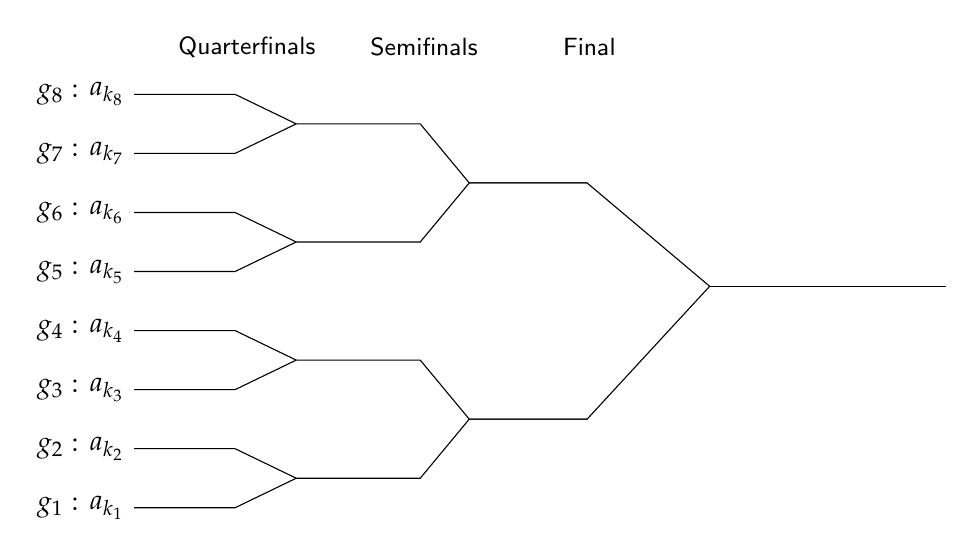
\begin{tikzpicture}[scale=.75]
\foreach \n in {1,2,3,4,5,6,7,8}
  \node (\n) at (0,\n*10mm) {$g_{\n}:$};
\foreach \n in {1,2,3,4}
  \node[inner sep=-4pt] (r\n) at (40mm,-5mm+\n*20mm) {};
\foreach \n/\r in {1/1,2/1,3/2,4/2,5/3,6/3,7/4,8/4}
  \draw (\n) --
     node[very near start,fill=white] {$a_{k_{\n}}$} +(30mm,0)
     -- ($(r\r)+(1pt,0)$);
\foreach \n/\v in {1/25mm,2/65mm}
  \node[inner sep=-5pt] (rr\n) at (70mm,\v) {};
\foreach \n/\r in {1/1,2/1,3/2,4/2}
  \draw ($(r\n)+(1pt,0)$) -- ++(21mm,0) -- 
  ($(rr\r)+(-1pt,0)$) -- ++(20mm,0);
\node[inner sep=-5pt] (rrr) at ($(rr1)+(40mm,22.5mm)$) {};
\foreach \n/\r in {1,2}
 \draw ($(rr\n)+(19.6mm,0)$) -- ($(rrr)+(1pt,0)$); 
\draw ($(rrr)+(1pt,0)$) -- +(40mm,0);
\node at (32mm,88mm) {\textsf{\small Quarterfinals}};
\node at (62mm,88mm) {\textsf{\small Semifinals}};
\node at (90mm,88mm) {\textsf{\small Final}};
\end{tikzpicture}
\end{center}
\caption{A tournament schedule}\label{f.tournament}
\end{figure}
\end{prob}

\newpage

\solution{}

\ans{1}
If $a_1$ is assigned to one of the games $\{g_1,g_2,g_3,g_4\}$ none of the other players assigned to these games will reach the final, so $a_2$ must be assigned to one of $\{g_5,g_6,g_7,g_8\}$. The temptation is to conclude that the probability of $a_2$ being the runner-up is $1/2$ since $a_2$ must be assigned to one of the four games $\{g_1,g_2,g_3,g_4\}$. However, whatever game $a_1$ is  assigned to, $a_2$ will be the runner up only if he is assigned to one of the four \emph{remaining} seven games so the probability is $4/7$.

\ans{2} Similarly, of the $2^n-1$ games that $a_1$ is not assigned to, $a_2$ must be assigned to one of the $2^{n-1}$ games not in the same half as $a_1$. Therefore:
\[
P(a_1,a_2\;\textsf{playing each other in the final})=\frac{2^{n-1}}{2^n-1}\,.
\]

\textbf{Simulation}
\begin{verbatim}
For   8 players:
Probability a2 is runner-up                = 0.5714
Proportion of games where a2 is runner-up  = 0.5707
For  32 players:
Probability a2 is runner-up                = 0.5161
Proportion of games where a2 is runner-up  = 0.5184
For 128 players:
Probability a2 is runner-up                = 0.5039
Proportion of games where a2 is runner-up  = 0.5060
\end{verbatim}

%%%%%%%%%%%%%%%%%%%%%%%%%%%%%%%%%%%%%%%%%%%%%%%%%%%%%%%%%%%%%

\begin{prob}{Twin knights\annotate{D}}

Eight players $\{a_1,\ldots,a_8\}$ are randomly assigned to play games $\{g_1,\ldots,g_8\}$ in a tournament (Figure~\ref{f.tournament}). Let $P(i,j)$ be the probability that $a_i$ wins against $a_j$. For all $i,j$, $P(i,j)=P(j,i)=1/2$.

\que{1} What is the probability that $a_1,a_2$ play each other?

\que{2} If there are $2^n$ players what is the probability that $a_1,a_2$ play each other?
\end{prob}

\solution{}

\ans{1} Without loss of generality assign $a_1$ to $g_1$. Consider the different possibilities that $a_1,a_2$ play each other. With probability $1/7$, $a_2$ is assigned to $g_2$. With probability $2/7$, $a_2$ is assigned to $g_3$ or $g_4$, but $a_2$ doesn't play $a_1$ unless \emph{both} of them win their first game, so we need to multiply the probability of this assignment by $1/4$. With probability $4/7$, $a_2$ is assigned to $g_5,g_6,g_7,g_8$, but $a_2$ doesn't play $a_1$ unless \emph{both} of them win their first two  games, so we need to multiply the probability of this assignment by $1/16$. Therefore:
\[
P(a_1, a_2\;\textsf{play each other})=\frac{1}{7} + \frac{1}{4}\cdot \frac{2}{7} + \frac{1}{16}\cdot \frac{4}{7} =\frac{1}{4}\,.
\]

\ans{2}
Let $P_n$ be the probability that in a tournament with $2^n$ players $a_1$ and $a_2$ play each other. We have shown that $P_3=1/4$. What about $P_4$? Using the same approach:
\begin{eqn}
P_4 &=& \frac{1}{15} + \frac{1}{4}\cdot \frac{2}{15}  + \frac{1}{16}\cdot \frac{4}{15}  + \frac{1}{64}\cdot \frac{8}{15} \\
&=&\frac{1}{15}\left(1+\frac{1}{2}+\frac{1}{4}+\frac{1}{8}\right)=\frac{1}{8}\,.
\end{eqn}%
It is reasonable to conjecture that $P_n=1/2^{n-1}$.

\textbf{Proof 1:} Using the same approach and the formula for the sum of a geometric series:
\begin{eqn}
P_n&=&\frac{1}{2^n-1}\sum_{i=0}^{n-1}2^i\cdot \left(\frac{1}{2}\right)^{2i}\\
&=&\frac{1}{2^n-1}\sum_{i=0}^{n-1}2^{-i}\\
&=&\frac{1}{2^n-1}
  \left(
    \frac{1-(1/2)^{(n-1)+1}}
         {1-(1/2)}
  \right)=\frac{1}{2^{n-1}}\,.
\end{eqn}%

\textbf{Proof 2:} By induction. The base case is $P_3=1/4=1/2^{3-1}$.

There are two inductive steps:

\textit{Case 1:} $a_1$ and $a_2$ are assigned to different halves of the tournament:
\[
P(a_1,a_2\;\textsf{assigned to different halves})=\frac{2^{n-1}}{2^n-1}\,.
\]
They can only meet in the final game and therefore both must win all of their $n-1$ games:
\begin{equation}\label{eq.17a}
P(a_1,a_2\;\textsf{meet if assigned to different halves})=\frac{2^{n-1}}{2^n-1} \left(\frac{1}{2}\right)^{n-1} \left(\frac{1}{2}\right)^{n-1}=\frac{2^{-(n-1)}}{2^n-1}\,.
\end{equation}
\textit{Case 2:} $a_1$ and $a_2$ are assigned to the same half of the tournament:
\[
P(a_1,a_2\;\textsf{assigned to the same half})=\frac{2^{n-1}-1}{2^n-1}\,.
\]
Since both players are in the same half the problem has been reduced to determining $P_{n-1}$. By the inductive hypothesis:
\begin{equation}\label{eq.17b}
P(a_1,a_2\;\textsf{meet if assigned to the same half})=\frac{2^{n-1}-1}{2^n-1}\cdot \frac{1}{2^{n-2}}=\frac{2^{1}-2^{-(n-2)}}{2^n-1}\,.
\end{equation}
Combining Equations~\ref{eq.17a}, \ref{eq.17b} gives:
\[
\renewcommand*{\arraystretch}{2.2}
\begin{array}{rcl}
P_n&=&\disfrac{2^{-(n-1)}}{2^n-1}+\disfrac{2^{1}-2^{-(n-2)}}{2^n-1}\\
&=&\disfrac{2^{n-1}}
        {2^{n-1}}\cdot 
   \disfrac{2^{-(n-1)}+2^{1}-2^{-(n-2)}}
        {2^n-1}\\
&=&\disfrac{1}
        {2^{n-1}}\cdot 
   \disfrac{2^0+2^n-2^1}
        {2^n-1}=\disfrac{1}{2^{n-1}}\,.
\end{array}
\]

\textbf{Simulation}
\begin{verbatim}
For   8 players:
Probability that a1, a2 meet = 0.2500
Proportion a1, a2 meet       = 0.2475
For  32 players:
Probability that a1, a2 meet = 0.0625
Proportion a1, a2 meet       = 0.0644
For 128 players:
Probability that a1, a2 meet = 0.0156
Proportion a1, a2 meet       = 0.0137
\end{verbatim}

%%%%%%%%%%%%%%%%%%%%%%%%%%%%%%%%%%%%%%%%%%%%%%%%%%%%%%%%%%%%%

\begin{prob}{An even split at coin tossing}
\que{1} Toss a fair coin $20$ times. What is the probability of obtaining $10$ heads?

\que{2} Toss a fair coin $40$ times. What is the probability of obtaining $20$ heads?
\end{prob}

\solution{}

\ans{1} Since the coin is fair the probability of obtaining $10$ heads in $20$ tosses is given by the binomial distribution:
\[
P(10\;\textsf{heads in}\; 20\; \textsf{tosses})={20 \choose 10} \left(\frac{1}{2}\right)^{10}\left(\frac{1}{2}\right)^{10} \approx 0.1762\,.
\]

\ans{2} You might expect the probability to be the same before but:
\[
P(20\;\textsf{heads in}\; 40\; \textsf{tosses})={40 \choose 20} \left(\frac{1}{2}\right)^{20}\left(\frac{1}{2}\right)^{20}\approx 0.1254\,.
\]
By the law of large numbers the numbers of heads and tails will be ``roughly'' equal \cite[Section~8.4]{ross}, but they are unlikely to be exactly the same, and this event becomes less likely as the number of tosses increases.

\newpage

\textbf{Simulation}
\begin{verbatim}
Probability of 10 heads for  20 tosses = 0.1762
Proportion  of 10 heads for  20 tosses = 0.1790
Probability of 20 heads for  40 tosses = 0.1254
Proportion  of 20 heads for  40 tosses = 0.1212
Probability of 50 heads for 100 tosses = 0.0796
Proportion  of 50 heads for 100 tosses = 0.0785
\end{verbatim}

%%%%%%%%%%%%%%%%%%%%%%%%%%%%%%%%%%%%%%%%%%%%%%%%%%%%%%%%%%%%%

\begin{prob}{Isaac Newton helps Samuel Pepys}
\que{1} What is the probability of obtaining \emph{at least one} $6$ when $6$ dice are thrown?

\que{2} What is the probability of obtaining \emph{at least two} $6$'s when $12$ dice are thrown?

\que{3} Develop a formula for the probability of obtaining at least $n$ $6$'s when $6n$ dice are thrown.
\end{prob}

\solution{}

\ans{1} The probability is the complement of the probability of obtaining zero $6$'s in $6$ throws:
\[
P(\textsf{at least one}\; 6)=1-\left(\frac{5}{6}\right)^6\approx 0.6651\,.
\]

\ans{2} The probability is the complement of the probability of obtaining zero or one $6$'s in $12$ throws:
\[
P(\textsf{at least two}\;6\textsf{s})=1-\left(\frac{5}{6}\right)^{12}-{12\choose 1}\left(\frac{1}{6}\right)^{1}\left(\frac{5}{6}\right)^{11}\approx 0.6187\,.
\]
This event is less probable than the previous one.

\ans{3} The probability is the complement of the probability of obtaining less than $n$ $6$'s in $6n$ throws:
\begin{eqn}
P(\textsf{at least}\;n\;6\textsf{s})&=&
  1-{6n \choose 0}\left(\frac{1}{6}\right)^0\left(\frac{5}{6}\right)^{6n-0}-
  {6n\choose 1}\left(\frac{1}{6}\right)^{1}\left(\frac{5}{6}\right)^{6n-1}-\cdots\\
&=&1-\sum_{i=0}^{n-1}{6n\choose i}\left(\frac{1}{6}\right)^{i}\left(\frac{5}{6}\right)^{6n-i}\,.
\end{eqn}%

\textbf{Simulation}
\begin{verbatim}
For   6 dice to throw  1 sixes:
Probability = 0.6651
Proportion  = 0.6566
For  12 dice to throw  2 sixes:
Probability = 0.6187
Proportion  = 0.6220
For  18 dice to throw  3 sixes:
Probability = 0.5973
Proportion  = 0.5949
For  96 dice to throw 16 sixes:
Probability = 0.5424
Proportion  = 0.5425
For 360 dice to throw 60 sixes:
Probability = 0.5219
Proportion  = 0.5250
\end{verbatim}

%%%%%%%%%%%%%%%%%%%%%%%%%%%%%%%%%%%%%%%%%%%%%%%%%%%%%%%%%%%%%

\begin{prob}{The three-cornered duel\annotate{D}}
$A,B,C$ fight a sequence of duels. Each of them has a fixed probability of winning a duel regardless of who the opponent is:
\[
P(A)=0.3,\quad P(B)=1, \quad P(C)=0.5\,.
\]
A person who is hit no longer participates in the duels. The shots are fired one at a time sequentially in the order $A,B,C$. If two opponents are still standing the shooter can decide whom to fire at. Assume that each person makes the optimal decision for each duel.

\que{1} What is $A$'s best strategy?

\que{2} Suppose that $A$ fires the first shot into the air. Is this a better strategy?

\textbf{Hint:} Give a formal definition for one strategy is better than another.

\textbf{Hint:} Compute the conditional probabilities of $A$ winning depending on whether $A$ chooses to shoot first at $B$ or $C$.
\end{prob}

\solution{}

Let $I_X$ be the indicator variable for $X$ winning the sequence of duels:
\[
I_X=
\left\{
\begin{array}{ll}
1,\quad X\;\textsf{wins the sequence of duels}\\
0, \quad X\; \textsf{loses the sequence of duels}\,.
\end{array}
\right.
\]
Strategy $s_1$ for $X$ is better strategy $s_2$ if the expectation of $I_X$ is greater for $s_1$ than for $s_2$.

Notation: \duel{X}{H}{Y} denotes that $X$ shoots at $Y$ and hits. \duel{X}{M}{Y} denotes that $X$ shoots at $Y$ and misses.

\ans{1}
Compute the conditional probabilities of $A$ winning.

\textit{Case 1:} $A$ chooses to shoot first at $C$.

If \duel{A}{M}{C} (probability $0.7$) then \duel{B}{H}{C} since $C$ is more dangerous than $A$. $A$ now shoots again at $B$ with probability $0.3$ of hitting, but if $A$ misses then \duel{B}{H}{A} with probability $1$ and $A$ loses.

If \duel{A}{H}{C} (probability $0.3$) then \duel{B}{H}{A} with probability $1$ and $A$ loses.

\vspace*{-3ex}
\[
\renewcommand*{\arraystretch}{2.5}
\begin{array}{l}
E(A \;\textsf{wins}\;|A\;\textsf{chooses to shoot first at}\;C) =\\
%
\qquad\quad \overbrace{1\cdot (0.7\cdot 1 \cdot 0.3)}^%
{\duelmath{A}{M}{C}, \duelmath{B}{H}{C}, \duelmath{A}{H}{B}}\; +
%
\overbrace{0\cdot (0.7\cdot 1\cdot 0.7\cdot 1)}^%
{\duelmath{A}{M}{C},  \duelmath{B}{H}{C}, \duelmath{A}{M}{B}, \duelmath{B}{H}{A}}+
%
\;\;\overbrace{0\cdot (0.3\cdot 1)}^%
{\duelmath{A}{H}{C}, \duelmath{B}{H}{A}}=0.2100\,.
\end{array}
\]
\textit{Case 2:} $A$ chooses to shoot first at $B$.

If \duel{A}{M}{B} (probability $0.7$) then as before \duel{B}{H}{C} and $A$ has one more chance to hit $B$ (probability $0.3$), otherwise \duel{B}{H}{A} with probability $1$ and $A$ loses.

If \duel{A}{H}{B} (probability $0.3$) then $A,C$ alternately shoot at each other until one is hit. The possibilities are:
\[
\begin{array}{ll}
(1)&C\stackrel{H}{\longrightarrow}A\\
(2)&C\stackrel{M}{\longrightarrow}A \stackrel{H}{\longrightarrow}C\\
(3)&C\stackrel{M}{\longrightarrow}A \stackrel{M}{\longrightarrow}C\stackrel{H}{\longrightarrow}A\\
(4)&C\stackrel{M}{\longrightarrow}A \stackrel{M}{\longrightarrow}C\stackrel{M}{\longrightarrow}A\stackrel{H}{\longrightarrow}C\\
(5)&C\stackrel{M}{\longrightarrow}A \stackrel{M}{\longrightarrow}C\stackrel{M}{\longrightarrow}A\stackrel{M}{\longrightarrow}C\stackrel{H}{\longrightarrow}A\\
(6)&C\stackrel{M}{\longrightarrow}A \stackrel{M}{\longrightarrow}C\stackrel{M}{\longrightarrow}A\stackrel{M}{\longrightarrow}C\stackrel{M}{\longrightarrow}A\stackrel{H}{\longrightarrow}C\\
&\cdots
\end{array}
\]
The probability of $A$ wins by eventually hitting $C$ is the sum of the probabilities of the even-numbered scenarios in the list:
\begin{eqn}
P(A\;\textsf{wins} \;| A\; \textsf{hits}\;B )&=&(0.5 \cdot 0.3) + \\
&&(0.5 \cdot 0.7) (0.5 \cdot 0.3) + \\
&&(0.5 \cdot 0.7) (0.5 \cdot 0.7) (0.5 \cdot 0.3)+ \cdots\\
&=&0.15 \sum_{i=0}^{\infty} 0.35^i= \frac{0.15}{1-0.35}=\frac{3}{13}\approx 0.2308\,.
\end{eqn}%
Similarly, the probability of $C$ winning is $\disfrac{0.5}{1-0.35}=\disfrac{10}{13}\approx 0.7692$.

The expectation is:
\vspace*{-1ex}
\[
\renewcommand*{\arraystretch}{1.5}
\begin{array}{l}
E(A \;\textsf{wins}) =E(A \;\textsf{wins}\;|\;A\;\textsf{misses}\;B) + E(A \;\textsf{wins}\;|\;A\;\textsf{hits}\;B)=\\
\qquad\qquad
\overbrace{1\cdot (0.7\cdot 1\cdot 0.3)}%
^{A\stackrel{M}{\longrightarrow}B, B\stackrel{H}{\longrightarrow}C, A\stackrel{H}{\longrightarrow}B}\;+
%
\overbrace{0\cdot (0.7\cdot 1\cdot 0.7\cdot 1)}%
^{A\stackrel{M}{\longrightarrow}B,
B\stackrel{H}{\longrightarrow}C,
A\stackrel{M}{\longrightarrow}B,
B\stackrel{H}{\longrightarrow}A}\; +
%
\overbrace{1\cdot 0.2308}%
^{A\stackrel{H}{\longrightarrow}B,
C\stackrel{H}{\longleftrightarrow*}A,
A\stackrel{H}{\longrightarrow}C}\; +\\
%
\qquad\;\,\overbrace{0\cdot 0.7692}%
^{A\stackrel{H}{\longrightarrow}B,
C\stackrel{H}{\longleftrightarrow*}A,
C\stackrel{H}{\longrightarrow}A}
\approx \; 0.2792\,,
\end{array}
\]
which is higher than the expectation of winning by shooting at $C$ first.

\ans{2} If $A$ shoots into the air not hitting anyone (probability $1$) then $B\stackrel{H}{\longrightarrow}C$ with probability $1$ and $A$ can try to hit $B$ with probability $0.3$. The expectation is:
\[
E(A \;\textsf{wins}|A\;\textsf{shoots in the air}) = 1\cdot (1\cdot 1 \cdot 0.3) + 0\cdot(1\cdot 1\cdot 0.7)=0.3\,,
\]
which is higher than the expectation for the other two strategies!

\textbf{Simulation}
\begin{verbatim}
For A fires first at C:
Expectation of wins = 0.2100
Average wins        = 0.2138
For A fires first at B:
Expectation of wins = 0.2792
Average wins        = 0.2754
For A fires in the air:
Expectation of wins = 0.3000
Average wins        = 0.3000
\end{verbatim}

%%%%%%%%%%%%%%%%%%%%%%%%%%%%%%%%%%%%%%%%%%%%%%%%%%%%%%%%%%%%%

%% !TeX root = mos-en.tex

%%%%%%%%%%%%%%%%%%%%%%%%%%%%%%%%%%%%%%%%%%%%%%%%%%%%%%%%%%%%%

\refstepcounter{problem}  % 11. Silent cooperation

%%%%%%%%%%%%%%%%%%%%%%%%%%%%%%%%%%%%%%%%%%%%%%%%%%%%%%%%%%%%%

\refstepcounter{problem}  % 12. Quo vadis?

%%%%%%%%%%%%%%%%%%%%%%%%%%%%%%%%%%%%%%%%%%%%%%%%%%%%%%%%%%%%%

\begin{prob}{The prisoner's dilemma\annotate{D}}

Three prisoners $A,B,C$ are eligible for parole. The parole board will release two of them with equal probability for $\{A,B\}, \{A,C\}, \{B,C\}$, so the probability that $A$ will be released is $2/3$. Prisoner $A$ is told the name of one of the other prisoners who will be released. If he is told that prisoner $B$ will be released, what is the probability that $A$ too will be released?

For a comprehensive article on the prisoner's dilemma problem and the related Monty Hall problem see \cite{carlton}.
\end{prob}

\solution{1}

Let $P(A), P(B), P(C)$ be the probabilities that $A,B,C$ are released. $A$ is interested in the conditional probability $P(A|B)$ of his being released if $B$ will be released:
\[
P(A|B) = \frac{P(A\cap B)}{P(B)} = \frac{1/3}{2/3}=\frac{1}{2}\,.
\]
But that is \emph{not} the correct conditional probability! Let $R_{AB}$ be the event that $A$ is \emph{told} that $B$ will be released. The probability that must be computed is $P(A|R_{AB})$:
\[
P(A|R_{AB}) = \frac{P(A\cap R_{AB})}{P(R_{AB})}\,.
\]
We assume that the report of $B$'s release is true so:
\[
P(A\cap R_{AB})=P(\{A,B\})=\disfrac{1}{3}\,.
\]
Now:
\[
P(R_{AB})=P(\{A,B\})+P(\{B,C\})=\disfrac{1}{3}+\disfrac{1}{2}\cdot \disfrac{1}{3}=\disfrac{1}{2}\,.
\]
If $\{B,C\}$ are to be released, $A$ could be told that either $B$ or $C$ is to be released, hence the factor of $1/2$. Therefore:
\[
P(A|R_{AB}) = \frac{P(A\cap R_{AB})}{P(R_{AB})} = \disfrac{1/3}{1/2}=\disfrac{2}{3}\,,
\]
so if $A$ is told that $B$ will be released the probability that he will be released does not change.

\solution{2}

There are four possible events:
\begin{description}
\item[$e_1$:] $A$ is told that $B$ will be released and $\{A,B\}$ are released. 
\item[$e_2$:] $A$ is told that $C$ will be released and $\{A,C\}$ are released. 
\item[$e_3$:] $A$ is told that $B$ will be released and $\{B,C\}$ are released. 
\item[$e_4$:] $A$ is told that $C$ will be released and $\{B,C\}$ are released. 
\end{description}
Each pair of prisoners has equal probability of being released so:
\[
P(e_1)=P(e_2)=P(e_3\cup e_4)=\frac{1}{3}\,.
\]
We assume that if $\{B,C\}$ are to be released, $A$ is told $B$ or $C$ with equal probability, so $P(e_3)=P(e_4)=1/6$. Therefore the probability that $A$ will be released given the event $R_{AB}=e_1\cup e_3$ that he is told that $B$ will be released is:
\[
P(A|R_{AB}) = \frac{P(e_1\cap(e_1\cup e_3))}{P(e_1\cup e_3)}=\frac{P(e_1)}{P(e_1\cup e_3)}=\frac{1/3}{(1/3)+(1/6)}=\frac{2}{3}\,.
\]

\solution{3}

A riddle attributed to Abraham Lincoln asks: ``If you call the tail of a dog a leg, how many legs does the dog have?'' The answer is that calling a tail a leg doesn't make it a leg, so the dog still has four legs. Clearly, whether $A$ knows $B$'s future doesn't change his chances of being released.

%%%%%%%%%%%%%%%%%%%%%%%%%%%%%%%%%%%%%%%%%%%%%%%%%%%%%%%%%%%%%

\begin{prob}{Collecting coupons\annotate{S}}
Given a sequence of boxes each of which contains coupons numbered $1$ to $5$. You randomly draw one coupon from each box one after another.

\que{1} What is the expectation of the number of coupons drawn until you have all five of the numbers?

\que{2} Develop a formula for the expectation for $n$ numbers.

\textbf{Hint:} Use the solution to Problem~4 on page~\pageref{p.four} and the approximation for the sum of harmonic numbers (page~\pageref{p.harmonic}).
\end{prob}

\solution{}

\ans{1} What is the expectation of the number of draws until you get a  number that is \emph{different from} all the previous ones? By  Problem~4 this is $1/p$ where $p$ is the probability of drawing a different number. For the first draw the probability is $1$ so the expectation is also $1$, for the second draw the probability is $4/5$ so expectation is $5/4$, and so on. Therefore:
\[
E(\textsf{all five numbers}) = \frac{5}{5}+\frac{5}{4} + \frac{5}{3} + \frac{5}{2} + \frac{5}{1} = \frac{}{} =\frac{1370}{120}\approx 11.4167\,.
\]
\ans{2} Use the same method and the approximation for $H_n$, the $n$th harmonic number (page~\pageref{p.harmonic}):
\[
E(\textsf{all}\;n \;\textsf{numbers}) = n\left(\frac{1}{n}+\frac{1}{n-1} + \cdots \frac{1}{2} + \frac{1}{1}\right) =nH_n\approx n\left(\ln n + \frac{1}{2n} + 0.5772\right)\,. 
\]
For $n=5$ this gives:
\[
E(\textsf{all five numbers}) =5H_5\approx 5(\ln 5 + \frac{1}{10} + 0.5772) \approx 11.4332\,.
\]

\textbf{Simulation}
\begin{verbatim}
For  5 coupons:
Expectation of draws = 11.9332
Average draws        = 11.4272
For 10 coupons:
Expectation of draws = 29.7979
Average draws        = 29.2929
For 20 coupons:
Expectation of draws = 72.4586
Average draws        = 72.2136
\end{verbatim}

%%%%%%%%%%%%%%%%%%%%%%%%%%%%%%%%%%%%%%%%%%%%%%%%%%%%%%%%%%%%%

\begin{prob}{The theater row\annotate{S}}
Arrange eight even numbers and seven odd numbers randomly in a row, for example:
\[
10\quad 12\quad 3\quad 2\quad 9\quad 6 \quad 1\quad 13\quad 7\quad 10\quad 3\quad 8\quad 8\quad 5\quad 20\,,
\]
which we can write as follows since the specific numbers are not important:
\[
E\quad E\quad O\quad E\quad O\quad E \quad O\quad O\quad O\quad E\quad O\quad E\quad E\quad O\quad E\,.
\]
What is the expectation of the number of even-odd or odd-even adjacent pairs?

In the example there are $10$ $EO$ or $OE$ adjacent pairs.

\textbf{Hint:} Consider each adjacent pair of separately. What is the probability that they are different?
\end{prob}

\solution{}

The following table shows the ten possible arrangements of three even and two odd numbers. The total number of different adjacent pairs is $24$ and the average is $24/10=2.4$.
\[
\begin{array}{l|r@{\hspace{2em}}|@{\hspace{2pt}}|@{\hspace{2em}}l|r}
\textsf{Arrangement}&\textsf{Pairs}&\textsf{Arrangement}&\textsf{Pairs}\\\hline
EEEOO & 1&
EEOEO & 3\\
EEOOE & 2&
EOEOE & 4\\
EOEEO & 3&
EOOEE & 1\\
OEEOE & 3&
OEEEO & 2\\
OEOEE & 3&
OOEEE & 1\\
\end{array}
\]
Return to the example with $15$ numbers. Let $P_d$ be the probability that a given pair in an arrangement is $EO$ or $OE$.  Then:
\[
P_d =P(EO) + P(OE) = \frac{8}{15}\cdot \frac{7}{14} + \frac{7}{15}\cdot \frac{8}{14} = 2\cdot \frac{8}{15}\cdot \frac{7}{14} = \frac{8}{15}\,.
\]
Let $E_d$ be the expectation of the number of pairs in an arrangement that are $EO$ or $OE$. Since an $(EO,OE)$ pair contributes $1$ to the count of different pairs and an $(EE,OO)$ pair contributes $0$:
\[
E_d =
\sum_{\textsf{\footnotesize pairs}} 1\cdot P_d= 14\cdot \frac{8}{15} \approx 7.4667\,.
\]

For ten numbers:
\begin{eqnarray*}
P_d &=& P(EO) + P(OE) = \frac{3}{5}\cdot \frac{2}{4} + \frac{2}{5}\cdot \frac{3}{4} = \frac{3}{5}\\
E_d &=& 4\cdot \frac{3}{5}=\frac{12}{5}=2.4\,.
\end{eqnarray*}

\textbf{Simulation}
\begin{verbatim}
For  5 places:
Expectation of different pairs = 2.4000
Average different pairs        = 2.3855
For 15 places:
Expectation of different pairs = 7.4667
Average different pairs        = 7.4566
For 27 places:
Expectation of different pairs = 13.4815
Average different pairs        = 13.4835
For 49 places:
Expectation of different pairs = 24.4898
Average different pairs        = 24.4725
\end{verbatim}

%%%%%%%%%%%%%%%%%%%%%%%%%%%%%%%%%%%%%%%%%%%%%%%%%%%%%%%%%%%%%

\begin{prob}{Will the second-best be runner-up?\annotate{S}}
Eight players in a tournament $\{a_1,\ldots,a_8\}$ are randomly assigned to play games $\{g_1,\ldots,g_8\}$ in a schedule such that player $a_{k_{i}}$ initially plays in position $g_{k_{i}}$ (Figure~\ref{f.tournament}). The players are ranked from the best $a_1$ to the worst $a_8$ and the better player will \emph{always} defeat her opponent.  Clearly $a_1$ will win the tournament.

\que{1} What is the probability that $a_2$ will be the runner-up by playing $a_1$ in the final round and losing to her?

\que{2} If there are $2^n$ players what is the probability that $a_2$ will be the runner-up by playing $a_1$ in the final round and losing to her?
\end{prob}
\begin{figure}[tb]
\begin{center}
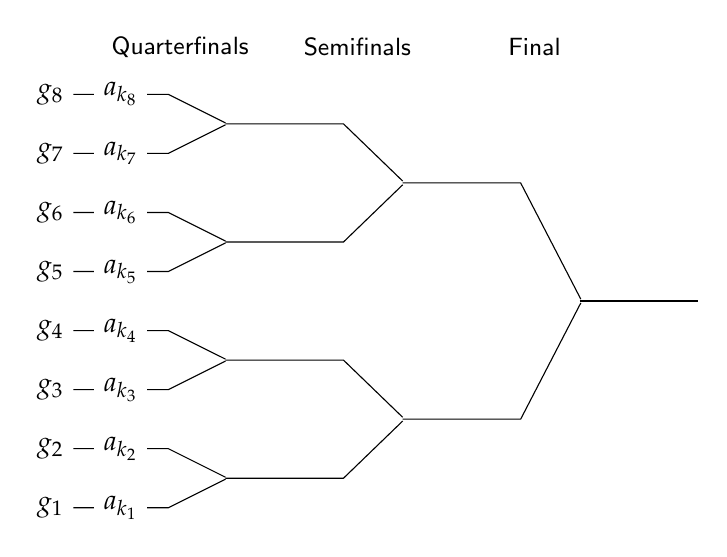
\begin{tikzpicture}[scale=.75]
\foreach \n in {1,2,3,4,5,6,7,8}
  \node (\n) at (0,\n*10mm) {$g_{\n}$};
\foreach \n in {1,2,3,4}
  \node[inner sep=-4pt] (r\n) at (30mm,-5mm+\n*20mm) {};
\foreach \n/\r in {1/1,2/1,3/2,4/2,5/3,6/3,7/4,8/4}
  \draw (\n) --
     node[fill=white] {$a_{k_{\n}}$} +(20mm,0) -- (r\r);
\foreach \n/\v in {1/25mm,2/65mm}
  \node[inner sep=-5pt] (rr\n) at (60mm,\v) {};
\foreach \n/\r in {1/1,2/1,3/2,4/2}
  \draw ($(r\n)+(-1pt,0)$) -- +(20mm,0) -- (rr\r);
\node[inner sep=-5pt] (rrr) at (90mm,45mm) {};
\foreach \n/\r in {1,2}
  \draw ($(rr\n)+(-1pt,0)$) -- +(20mm,0) -- (rrr); 
\draw ($(rrr)+(-1pt,0)$) -- +(20mm,0);
\node at (22mm,88mm) {\textsf{\small Quarterfinals}};
\node at (52mm,88mm) {\textsf{\small Semifinals}};
\node at (82mm,88mm) {\textsf{\small Final}};
\end{tikzpicture}
\end{center}
\caption{A tournament schedule}\label{f.tournament}
\end{figure}

\solution{}

\ans{1}
If $a_1$ is assigned to one of the games $\{g_1,g_2,g_3,g_4\}$ none of the other players assigned to these games will reach the final, so $a_2$ must be assigned to one of $\{g_5,g_6,g_7,g_8\}$. The temptation is to conclude that the probability of $a_2$ being the runner-up is $1/2$ since he must be assigned to one of the four games $\{g_1,g_2,g_3,g_4\}$. However, whatever game $a_1$ is  assigned to, $a_2$ will be the runner up only if he is assigned to one of four of the remaining seven games so the probability is $4/7$.

\ans{2} Similarly, of the $2^n-1$ games that $a_1$ is not assigned to, $a_2$ must be assigned to one of the $2^{n-1}$ games not in the same half as $a_1$. Therefore:
\[
P(a_1,a_2\;\textsf{playing each other in the final})=\frac{2^{n-1}}{2^n-1}\,.
\]

\textbf{Simulation}
\begin{verbatim}
For   8 players:
Probability a2 is runner-up                = 0.5714
Proportion of games where a2 is runner-up  = 0.5707
For  32 players:
Probability a2 is runner-up                = 0.5161
Proportion of games where a2 is runner-up  = 0.5184
For 128 players:
Probability a2 is runner-up                = 0.5039
Proportion of games where a2 is runner-up  = 0.5060
\end{verbatim}

%%%%%%%%%%%%%%%%%%%%%%%%%%%%%%%%%%%%%%%%%%%%%%%%%%%%%%%%%%%%%

\begin{prob}{Twin knights\annotate{D,S}}

Eight players in a tournament $\{a_1,\ldots,a_8\}$ are randomly assigned to play games $\{g_1,\ldots,g_8\}$ in a schedule such that $a_{k_{i}}$ initially plays in position $g_{k_{i}}$ (Figure~\ref{f.tournament}). For all $i,j$, the probability that $a_i$ wins in a game against $a_j$ is $1/2$ as is the probability that $a_j$ wins against $a_i$.

\que{1} What is the probability that $a_1,a_2$ play each other?

\que{2} If there are $2^n$ players, what is the probability that $a_1,a_2$ play each other?
\end{prob}

\solution{}

\ans{1} Without loss of generality assign $a_1$ to $g_1$. Consider the different possibilities that $a_1,a_2$ play each other. With probability $1/7$, $a_2$ is assigned to $g_2$. With probability $2/7$, $a_2$ is assigned to $g_3$ or $g_4$, but he doesn't play $a_1$ unless \emph{both} of them win their first game, so we need to multiply the probability of this assignment by $1/4$. With probability $4/7$, $a_2$ is assigned to $g_5,g_6,g_7,g_8$, but he doesn't play $a_1$ unless \emph{both} of them win their first two  games, so we need to multiply the probability of this assignment by $1/16$. Therefore:
\[
P(a_1, a_2\;\textsf{play each other})=\frac{1}{7} + \frac{1}{4}\cdot \frac{2}{7} + \frac{1}{16}\cdot \frac{4}{7} =\frac{1}{4}\,.
\]

\ans{2}
Let $P_n$ be the probability that in a tournament with $2^n$ players, $a_1$ and $a_2$ play each other. We have shown that $P_3=1/4$. What about $P_4$? Using the same approach:
\begin{eqnarray*}
P_4 &=& \frac{1}{15} + \frac{1}{4}\cdot \frac{2}{15}  + \frac{1}{16}\cdot \frac{4}{15}  + \frac{1}{64}\cdot \frac{8}{15} \\
&=&\frac{1}{15}\left(1+\frac{1}{2}+\frac{1}{4}+\frac{1}{8}\right)=\frac{1}{8}\,.
\end{eqnarray*}
It is reasonable to conjecture that $P_n=1/2^{n-1}$.

\textbf{Proof 1:} Using the same approach and the formula for the sum of a geometric series:
\begin{eqnarray*}
P_n&=&\frac{1}{2^n-1}\sum_{i=0}^{n-1}2^i\cdot \left(\frac{1}{2}\right)^{2i}\\
&=&\frac{1}{2^n-1}\sum_{i=0}^{n-1}2^{-i}\\
&=&\frac{1}{2^n-1}
  \left(
    \frac{1-\left(\frac{1}{2}\right)^{(n-1)+1}}
         {1-\frac{1}{2}}
  \right)=\frac{1}{2^{n-1}}\,.
\end{eqnarray*}

\textbf{Proof 2:} By induction. The base case is $P_3=1/4=1/2^{3-1}$.

There are two inductive steps:

\textit{Case 1:} $a_1$ and $a_2$ are assigned to different halves of the tournament:
\[
P(a_1,a_2\;\textsf{assigned to different halves})=\frac{2^{n-1}}{2^n-1}\,.
\]
They can only meet in the final game and therefore both must win all of their $n-1$ games:
\begin{equation}\label{eq.17a}
P(a_1,a_2\;\textsf{meet if assigned to different halves})=\frac{2^{n-1}}{2^n-1} \left(\frac{1}{2}\right)^{n-1} \left(\frac{1}{2}\right)^{n-1}=\frac{2^{-(n-1)}}{2^n-1}\,.
\end{equation}
\textit{Case 2:} $a_1$ and $a_2$ are assigned to the same half of the tournament:
\[
P(a_1,a_2\;\textsf{assigned to the same half})=\frac{2^{n-1}-1}{2^n-1}\,.
\]
Since both players are in the same half the problem has been reduced to determining $P_{n-1}$. By the inductive hypothesis:
\begin{equation}\label{eq.17b}
P(a_1,a_2\;\textsf{meet if assigned to the same half})=\frac{2^{n-1}-1}{2^n-1}\cdot \frac{1}{2^{n-2}}=\frac{2^{1}-2^{-(n-2)}}{2^n-1}\,.
\end{equation}
Combining Equations~\ref{eq.17a}, \ref{eq.17b} gives:
\[
\renewcommand*{\arraystretch}{2.2}
\begin{array}{rcl}
P_n&=&\disfrac{2^{-(n-1)}}{2^n-1}+\disfrac{2^{1}-2^{-(n-2)}}{2^n-1}\\
&=&\disfrac{2^{n-1}}
        {2^{n-1}}\cdot 
   \disfrac{2^{-(n-1)}+2^{1}-2^{-(n-2)}}
        {2^n-1}\\
&=&\disfrac{1}
        {2^{n-1}}\cdot 
   \disfrac{2^0+2^n-2^1}
        {2^n-1}=\disfrac{1}{2^{n-1}}\,.
\end{array}
\]

\textbf{Simulation}
\begin{verbatim}
For   8 players:
Probability that a1, a2 meet = 0.2500
Proportion a1, a2 meet       = 0.2475
For  32 players:
Probability that a1, a2 meet = 0.0625
Proportion a1, a2 meet       = 0.0644
For 128 players:
Probability that a1, a2 meet = 0.0156
Proportion a1, a2 meet       = 0.0137
\end{verbatim}

%%%%%%%%%%%%%%%%%%%%%%%%%%%%%%%%%%%%%%%%%%%%%%%%%%%%%%%%%%%%%

\begin{prob}{An even split at coin tossing\annotate{S}}
\que{1} If you toss a fair coin $20$ times, what is the probability of obtaining exactly $10$ heads?

\que{2} If you toss a fair coin $40$ times, what is the probability of obtaining exactly $20$ heads?
\end{prob}

\solution{}

\ans{1} Since the coin is fair the probability of obtaining $10$ heads in $20$ tosses is given by the binomial coefficient:
\[
P(10\;\textsf{heads in}\; 20\; \textsf{tosses})={20 \choose 10} \left(\frac{1}{2}\right)^{10}\left(\frac{1}{2}\right)^{10} \approx 0.1762\,.
\]

\ans{2} You might expect the probability to be the same as in the previous question, but:
\[
P(20\;\textsf{heads in}\; 40\; \textsf{tosses})={40 \choose 20} \left(\frac{1}{2}\right)^{20}\left(\frac{1}{2}\right)^{20}\approx 0.1254\,.
\]
By the law of large numbers the numbers of heads and tails will be ``roughly'' equal \cite[Section~8.4]{ross}, but they are unlikely to be exactly the same, and this event becomes less likely as the number of tosses increases.

\textbf{Simulation}
\begin{verbatim}
Probability of 10 heads for  20 tosses = 0.1762
Proportion  of 10 heads for  20 tosses = 0.1790
Probability of 20 heads for  40 tosses = 0.1254
Proportion  of 20 heads for  40 tosses = 0.1212
Probability of 50 heads for 100 tosses = 0.0796
Proportion  of 50 heads for 100 tosses = 0.0785
\end{verbatim}

%%%%%%%%%%%%%%%%%%%%%%%%%%%%%%%%%%%%%%%%%%%%%%%%%%%%%%%%%%%%%

\begin{prob}{Isaac Newton helps Samuel Pepys\annotate{S}}
\que{1} What is the probability of obtaining \emph{at least one} $6$ when $6$ dice are thrown?

\que{2} What is the probability of obtaining \emph{at least two} $6$s when $12$ dice are thrown?

\que{3} Develop a formula for the probability of obtaining at least $n$ $6$s when $6n$ dice are thrown.
\end{prob}

\solution{}

\ans{1} The probability is the complement of the probability of obtain zero $6$s in $6$ throws, which is the product of obtaining a number different from $6$ in all throws:
\[
P(\textsf{at least one}\; 6)=1-\left(\frac{5}{6}\right)^6\approx 0.6651\,.
\]

\ans{2} The probability is the complement of the probability of obtain zero or one $6$s in $12$ throws:
\[
P(\textsf{at least two}\;6\textsf{s})=1-\left(\frac{5}{6}\right)^{12}-{12\choose 1}\left(\frac{1}{6}\right)^{1}\left(\frac{5}{6}\right)^{11}\approx 0.6187\,.
\]
This event is less probable than the previous one.

\ans{3} The probability is the complement of the probability of obtain less than $n$ $6$s in $6n$ throws:
\begin{eqnarray*}
P(\textsf{at least}\;n\;6\textsf{s})&=&
  1-{6n \choose 0}\left(\frac{1}{6}\right)^0\left(\frac{5}{6}\right)^{6n-0}-
  {6n\choose 1}\left(\frac{1}{6}\right)^{1}\left(\frac{5}{6}\right)^{6n-1}-\cdots\\
&=&1-\sum_{i=0}^{n-1}{6n\choose i}\left(\frac{1}{6}\right)^{i}\left(\frac{5}{6}\right)^{6n-i}\,.
\end{eqnarray*}

\textbf{Simulation}
\begin{verbatim}
For   6 dice to throw  1 sixes:
Probability = 0.6651
Proportion  = 0.6566
For  12 dice to throw  2 sixes:
Probability = 0.6187
Proportion  = 0.6220
For  18 dice to throw  3 sixes:
Probability = 0.5973
Proportion  = 0.5949
For  96 dice to throw 16 sixes:
Probability = 0.5424
Proportion  = 0.5425
For 360 dice to throw 60 sixes:
Probability = 0.5219
Proportion  = 0.5250
\end{verbatim}

%%%%%%%%%%%%%%%%%%%%%%%%%%%%%%%%%%%%%%%%%%%%%%%%%%%%%%%%%%%%%

\begin{prob}{The three-cornered duel\annotate{S}}
$A,B,C$ fight a sequence of duels. Each of them has a fixed probability of winning a duel regardless of who the opponent is:
\[
P(A)=0.3,\quad P(B)=1, \quad P(C)=0.5\,.
\]
A person who is hit no longer participates in the duels. The shots are fired one at a time sequentially in the order $A,B,C$. If two opponents are still standing the shooter can decide whom to fire at. Assume that each person always makes an optimal decision.

\que{1} What is $A$'s optimal strategy?

\que{2} Suppose that $A$ fires the first shot into the air. Is this a better strategy?

\textbf{Hint:} Compute the conditional probabilities of $A$ winning depending on whether he chooses to shoot first at $B$ or $C$.
\end{prob}

\solution{}

Notation: $X\stackrel{H}{\longrightarrow}Y$ denotes that $X$ shoots at $Y$ and hits. $X\stackrel{M}{\longrightarrow}Y$ denotes that $X$ shoots at $Y$ and misses.

\ans{1}
Compute the conditional probabilities of $A$ winning.

\textit{Case 1:} $A$ chooses to shoot first at $C$.

If $A\stackrel{M}{\longrightarrow}C$ (probability $0.7$) then $B\stackrel{H}{\longrightarrow}C$ since $C$ is more dangerous than $A$. $A$ now shoots again at $B$ with probability $0.3$ of hitting, but if $A$ misses then $B\stackrel{H}{\longrightarrow}A$ with probability $1$ and $A$ loses.

If $A\stackrel{H}{\longrightarrow}C$ (probability $0.3$) then $B\stackrel{H}{\longrightarrow}A$ with probability $1$ and $A$ loses.

Compute the expectation with $1$ when $A$ wins and $0$ when $A$ loses:
\vspace*{-3ex}
\[
\renewcommand*{\arraystretch}{2.5}
\begin{array}{l}
E(A \;\textsf{wins}\;|A\;\textsf{chooses to shoot first at}\;C) =\\
%\qquad E(A \;\textsf{wins}\;|\;A\;\textsf{misses}\;C) + E(A \;\textsf{wins}\;|\;A\;\textsf{hits}\;C)=\\
\qquad \overbrace{1\cdot (0.7\cdot 0.3)}^{A\stackrel{M}{\longrightarrow}C, A\stackrel{H}{\longrightarrow}B}+ \overbrace{0\cdot (0.7\cdot 0.7\cdot 1)}^{A\stackrel{M}{\longrightarrow}C, A\stackrel{M}{\longrightarrow}B, B\stackrel{H}{\longrightarrow}A}+ \overbrace{0\cdot (0.3\cdot 1)}^{A\stackrel{M}{\longrightarrow}C, B\stackrel{H}{\longrightarrow}A}=0.2100\,.
\end{array}
\]
\textit{Case 2:} $A$ chooses to shoot first at $B$.

If $A\stackrel{M}{\longrightarrow}B$ (probability $0.7$) then as before $B\stackrel{H}{\longrightarrow}C$ and $A$ has one more chance to hit $B$ (probability $0.3$), otherwise $B\stackrel{H}{\longrightarrow}A$ with probability $1$ and $A$ loses.

If $A\stackrel{H}{\longrightarrow}B$ (probability $0.3$) then $A,C$ alternately shoot at each other until one is hit. The possibilities are:
\[
\begin{array}{ll}
(1)&C\stackrel{H}{\longrightarrow}A\\
(2)&C\stackrel{M}{\longrightarrow}A \stackrel{H}{\longrightarrow}C\\
(3)&C\stackrel{M}{\longrightarrow}A \stackrel{M}{\longrightarrow}C\stackrel{H}{\longrightarrow}A\\
(4)&C\stackrel{M}{\longrightarrow}A \stackrel{M}{\longrightarrow}C\stackrel{M}{\longrightarrow}A\stackrel{H}{\longrightarrow}C\\
(5)&C\stackrel{M}{\longrightarrow}A \stackrel{M}{\longrightarrow}C\stackrel{M}{\longrightarrow}A\stackrel{M}{\longrightarrow}C\stackrel{H}{\longrightarrow}A\\
(6)&C\stackrel{M}{\longrightarrow}A \stackrel{M}{\longrightarrow}C\stackrel{M}{\longrightarrow}A\stackrel{M}{\longrightarrow}C\stackrel{M}{\longrightarrow}A\stackrel{H}{\longrightarrow}C\\
&\cdots
\end{array}
\]
The probability of $A$ wins by eventually hitting $C$ is the sum of the probabilities of the even-numbered scenarios in the list:
\begin{eqnarray*}
P(A\;\textsf{wins} \;| A\; \textsf{hits}\;B )&=&(0.5 \cdot 0.3) + \\
&&(0.5 \cdot 0.7) (0.5 \cdot 0.3) + \\
&&(0.5 \cdot 0.7) (0.5 \cdot 0.7) (0.5 \cdot 0.3)+ \cdots\\
&=&0.15 \sum_{i=0}^{\infty} 0.35^i= \frac{0.15}{1-0.35}=\frac{3}{13}\approx 0.2308\,.
\end{eqnarray*}
Similarly, the probability of $C$ winning is $\disfrac{0.5}{1-0.35}=\disfrac{1}{13}\approx 0.0760$.

The expectation is:
\vspace*{-4ex}
\[
\renewcommand*{\arraystretch}{2.5}
\begin{array}{l}
E(A \;\textsf{wins}) =E(A \;\textsf{wins}\;|\;A\;\textsf{misses}\;B) + E(A \;\textsf{wins}\;|\;A\;\textsf{hits}\;B)=\\
\qquad
\overbrace{1\cdot (0.7\cdot 1\cdot 0.3)}%
^{A\stackrel{M}{\longrightarrow}B, B\stackrel{H}{\longrightarrow}C, A\stackrel{H}{\longrightarrow}B}+

\overbrace{0\cdot (0.7\cdot 1\cdot 0.7\cdot 1)}%
^{A\stackrel{M}{\longrightarrow}B, B\stackrel{H}{\longrightarrow}C,A\stackrel{M}{\longrightarrow}B,B\stackrel{H}{\longrightarrow}A} +

\overbrace{1\cdot (0.2308)}%
^{A\stackrel{H}{\longrightarrow}B, C\stackrel{H}{\longleftrightarrow*}A,C\stackrel{H}{\longrightarrow}A} +
\overbrace{0\cdot (0.3\cdot (0.0769))}%
^{A\stackrel{H}{\longrightarrow}B, C\stackrel{H}{\longleftrightarrow}A,C\stackrel{H}{\longrightarrow}A}
\approx\\
\qquad 0.2792\,,
\end{array}
\]
which is higher than the expectation of winning by shooting at $C$ first.

\ans{2} If $A$ shoots into the air not hitting anyone then $B\stackrel{H}{\longrightarrow}C$ with probability $1$ and $A$ can try to hit $B$ with probability $0.3$. The expectation is:
\[
E(A \;\textsf{wins}|A\;\textsf{shoots in the air}) = 1\cdot(0.3) + 0\cdot(0.7)=0.3\,,
\]
which is better than the expectation for the other two strategies!

\textbf{Simulation}
\begin{verbatim}
For A fires first at C:
Expectation of wins = 0.2100
Average wins        = 0.2138
For A fires first at B:
Expectation of wins = 0.2792
Average wins        = 0.2754
For A fires in the air:
Expectation of wins = 0.3000
Average wins        = 0.3000
\end{verbatim}

%%%%%%%%%%%%%%%%%%%%%%%%%%%%%%%%%%%%%%%%%%%%%%%%%%%%%%%%%%%%%

%% !TeX root = mos-he.tex

%%%%%%%%%%%%%%%%%%%%%%%%%%%%%%%%%%%%%%%%%%%%%%%%%%%%%%%%%%%%%%%%

\refstepcounter{problem}  % 41. The locomotive problem

%%%%%%%%%%%%%%%%%%%%%%%%%%%%%%%%%%%%%%%%%%%%%%%%%%%%%%%%%%%%%%%%

\begin{prob}{הקצה הקצר של המקל}{}{(The little end of the stick)}

אתה שובר מספר גדול של מקלות זכוכית באורך $1$ לשני חלקים. למקום השבירה התפלגות אחידה לאורך המקל.


\que{1} 
מה התוחלת של אורכו של החלק 
\textbf{הקטן}
יותר?

\que{2} 
מה התוחלת של היחס בין אורכו של החלק הקטן לאורכו של החלק הגדול?
\end{prob}
\solution{}

\ans{1}
ההסתברות שנקודת השבירה היא בצד השמאלי של המקל היא
$1/2$
שהיא גם ההסתברות שהנקודה בצד ימין. החלק הקטן יותר נמצא באותו צד שבו נמצאת נקודת השבירה. התוחלת של נדוקת השבירה היא באמצע בין קצה המקל לבין אמצע המקל:
\[
E(\textrm{יותר הקטן אורך}) = \frac{1}{2}\cdot\frac{1}{2}=\frac{1}{4}\,.
\]

\ans{2}
ללא הגבלת הכלליות הנח שנקודת השבירה נמצאת בצד הימני של המקל (איור%
~\ref{f.stick}).
היחס בין החלק הקטן והחלק הגדול הוא
$(1-x)/x$
ואורכו של החלק הגדול מתפלג אחיד בתוך
$(1/2,1)$. 
לכן:
\begin{eqn}
E(\textrm{יותר קטן / יותר גדול יחס})&=&\left(\frac{1}{1-(1/2)}\right)\int_{1/2}^1 \frac{1-x}{x} \,dx\\
&=& 2\int_{1/2}^1 \left(\frac{1}{x} -1\right) \,dx \\
&=& 2\left.(\ln |x| - x)\right|_{1/2}^1 = 2\ln 2 -1\approx 0.3863\,.
\end{eqn}
\begin{figure}[tb]
\begin{center}
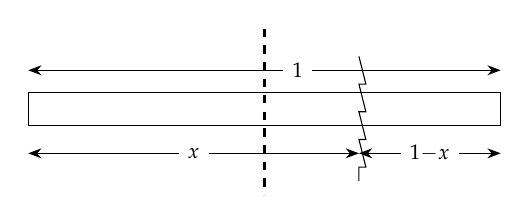
\begin{tikzpicture}
\draw (0,0) -- ++(6,0) -- ++(0,12pt) -- ++(-6,0) -- cycle;
\draw[<->] (0,20pt) --
  node[fill=white,xshift=12pt] {$\scriptstyle 1$} ++(6,0);
\draw[decorate,decoration=saw] (4.2,25pt) -- +(0,-45pt);
\draw[thick,dashed] (3,35pt) -- +(0,-60pt);
\draw[<->] (0,-10pt) --
  node[fill=white] {$\scriptstyle x$} (4.2,-10pt);
\draw[<->] (4.2,-10pt) --
  node[fill=white] {$\scriptstyle 1-x$} (6,-10pt);
\end{tikzpicture}
\end{center}
\caption{שבירת מקל לשני חלקים}\label{f.stick}
\end{figure}

\textbf{סימולציה}
\selectlanguage{english}
\begin{verbatim}
Expectation of length of smaller = 0.2500
Average length of smaller        = 0.2490
Expectation of smaller/larger    = 0.3863
Average smaller/larger           = 0.3845
\end{verbatim}
\selectlanguage{hebrew}

%%%%%%%%%%%%%%%%%%%%%%%%%%%%%%%%%%%%%%%%%%%%%%%%%%%%%%%%%%%%%%%%


\begin{prob}{המקל השבור}{D}{(The broken bar)}

אתה שובר מספר רב של מקלות זכוכית באורך 
$1$
בשתי נדוקות שבירה (איור%
~\ref{f.break1}).

\que{1} 
מה התוחלת של אורכו של החלק הקצר ביותר?

\que{2} 
מה התוחלת של אורכו של החלק הארוך ביותר?

\textbf{רמז:}
$x,y$
הם משתנים אקראים בלתי-תלויים בהתפלגות אחידה בתוך 
$(0,1)$.
ניתן להציג כל זוג
$(x,y)$
כנקודה בריבוע
$(0,1)\times (0,1)$ 
(איור%
~\ref{f.break2}).
מה ההסתברות ש-%
$(x,y) < (.5,.25)$? 

\textbf{Hint:}
עבור 
\que{1}
הנח שהחלק השמאלי הוא הקצר ביותר ועבור 
\que{2}
הנח שהחלק השמאלי הוא בארוך ביותר.
\begin{figure}[tb]
\centering
\selectlanguage{hebrew}
\subcaptionbox{%
חלוקת מקל לשני חלקים%
\label{f.break1}}
[.45\textwidth]
{
\centering
\begin{tikzpicture}[scale=.75]
\draw (0,0) node[below left] {$0$} --
  ++(6,0) node[below right] {$1$} --
  ++(0,12pt) -- ++(-6,0) -- cycle;
\draw[<->] (0,20pt) --
  node[fill=white] {$\scriptstyle 1$} ++(6,0);
\draw[decorate,decoration=saw] (1.8,25pt) -- +(0,-45pt);
\draw[decorate,decoration=saw] (4.7,25pt) -- +(0,-45pt);
\node[below left] at (1.8,0) {$x$};
\node[below left] at (4.7,0) {$y$};
\path (0,-3.5) rectangle +(0,3.5);
\end{tikzpicture}
}
\hspace{3em}
\subcaptionbox{%
יצוג האורכים במעגל היחידה%
\label{f.break2}}
[.45\textwidth]
{
\centering
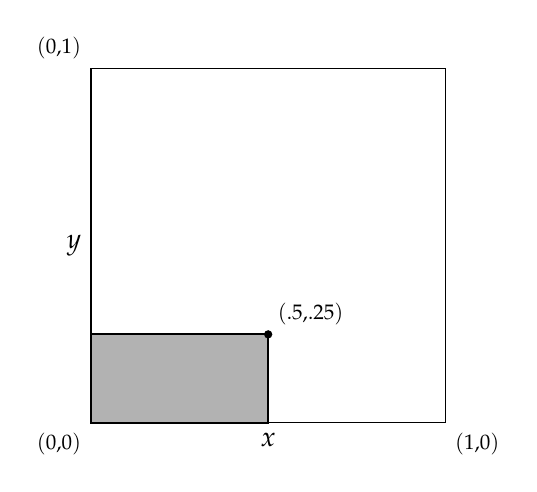
\begin{tikzpicture}[scale=.75]
\draw (-3,-3) rectangle +(6,6);
\draw[thick,fill=white!70!black] (-3,-3) -- ++(0,1.5) -- 
  ++(3,0) -- ++(0,-1.5) -- cycle;
\path (-3,-3) node[below left] {$\scriptstyle (0,0)$} --
  node[below] {$x$} (3,-3)
  node[below right] {$\scriptstyle (1,0)$};
\path (-3,-3) -- node[left] {$y$} (-3,3)
  node[above left] {$\scriptstyle (0,1)$};
\fill (0,-1.5) circle [radius=2pt]
  node[above right] {$\scriptstyle (.5,.25)$};
\end{tikzpicture}
}
\end{figure}
\end{prob}
\solution{}

\ans{1}
ללא הגבלת הכלליות הנח שהחלק השמאלי שאורכו 
$x$
הוא החלק הקצר ביותר. מכאן ש-%
$x<y-x$
ו-%
$x < 1-y$
שניתן לפשט ולקבל
$2x<y$
ו-%
$x+y<1$.

איור%
~\ref{f.shaded1}
מראה את הקווים
$y=2x$
(אדום) ו-%
$y=1-x$
(כחול). כדי לאמת את אי-השוויונות, 
$(x,y)$
חייבת להיות באיזור באפור לשמאל לשני הקווים. ניתן לחשב את נקודת החיתוך
$(1/2,2/3)$
על ידי פתרון שתי המשוואות.

הערכים של 
$(x,y)$
נמצאים בריבוע
$(0,1)\times(0,1)$,
ולכן יש לחשב את התוחלת מעל לתת-קבוצה האפורה של הריבוע על ידי חילוק האינטגרל בשטח של האיזור האפור
$\frac{1}{2} (\frac{1}{3}\cdot 1)=\frac{1}{6}$:
\begin{eqn}
E(x)&=& \frac{1}{1/6}\int_{0}^{1/3} x [(1-x)-2x]\,dx\\
&=&\int_{0}^{1/3} (6x -18x^2)\,dx\\
&=&\left. (3x^2-6x^3)\right|_0^{1/3}=\disfrac{2}{18}\approx 0.1111\,.
\end{eqn}

\begin{figure}[tb]
\centering
\selectlanguage{hebrew}
\subcaptionbox{%
איזור אפור עבור המקל הקצר ביותר%
\label{f.shaded1}}
[.45\textwidth]
{
\centering
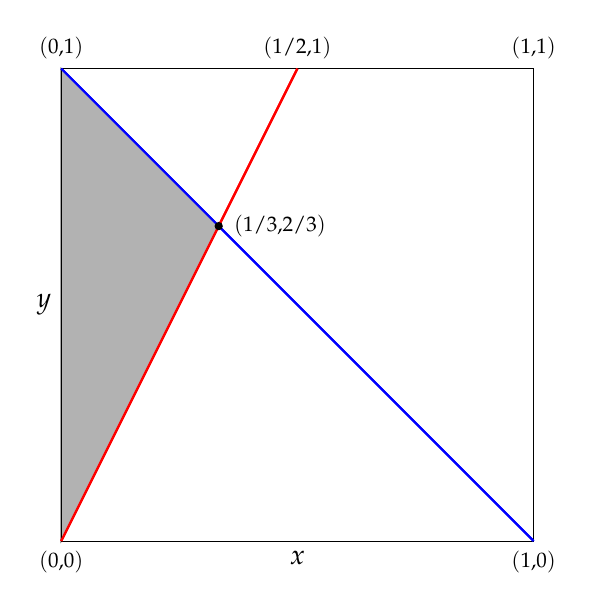
\begin{tikzpicture}[scale=1]
\draw (-3,-3) rectangle +(6,6);
\path (-3,-3) node[below] {$\scriptstyle (0,0)$} --
  node[below] {$x$} (3,-3)
  node[below] {$\scriptstyle (1,0)$};
\path (-3,-3) -- node[left] {$y$} (-3,3)
  node[above] {$\scriptstyle (0,1)$};
\draw[red,thick]  (-3,-3) -- (0,3);
\draw[blue,thick] (-3,3)  -- (3,-3);
\coordinate (P) at (-1,1);
\draw[fill=white!70!black] (-3,-3) -- (P) -- 
  (-3,3) -- cycle;
\draw[red,thick]  (-3,-3) -- (0,3);
\draw[blue,thick] (-3,3)  -- (3,-3);
\fill (P) circle[radius=1.5pt]
  node[right,xshift=2pt] {$\scriptstyle (1/3,2/3)$};
%\draw[thick,dotted] (-3,-3) -- (3,3);
\node[above] at(0,3) {$\scriptstyle (1/2,1)$};
\node[above] at(3,3) {$\scriptstyle (1,1)$};
\end{tikzpicture}
}
\hspace{1em}
\subcaptionbox{%
איזור אפור עבור המקל הארוך ביותר%
\label{f.shaded2}}
[.45\textwidth]
{
\centering
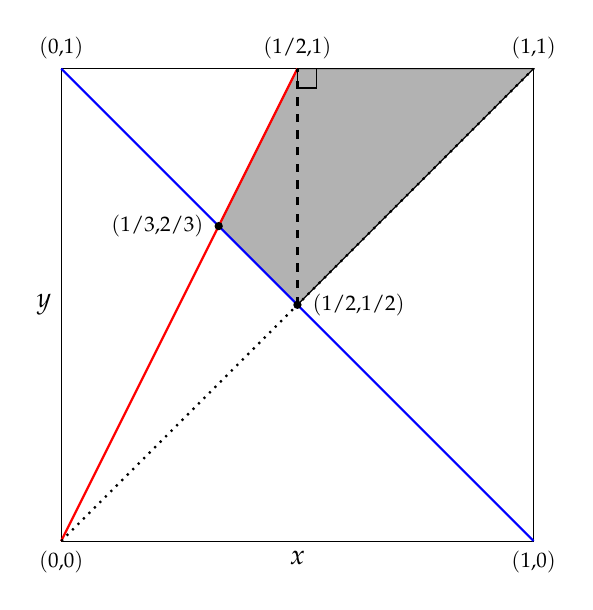
\begin{tikzpicture}[scale=1]
\draw (-3,-3) rectangle +(6,6);
\path (-3,-3) node[below] {$\scriptstyle (0,0)$} --
  node[below] {$x$} (3,-3)
  node[below] {$\scriptstyle (1,0)$};
\path (-3,-3) -- node[left] {$y$} (-3,3)
  node[above] {$\scriptstyle (0,1)$};
\coordinate (P) at (-1,1);
\coordinate (Q) at (0,0);
\draw[fill=white!70!black] (3,3) -- (Q) -- 
  (P) -- (0,3) -- cycle;
\draw[red,thick]  (-3,-3) -- (0,3);
\draw[blue,thick] (-3,3)  -- (3,-3);
\fill (P) circle[radius=1.5pt]
  node[left,xshift=-2pt] {$\scriptstyle (1/3,2/3)$};
\draw[thick,dotted] (-3,-3) -- (3,3);
\fill (Q) circle[radius=1.5pt]
  node[right,xshift=2pt] {$\scriptstyle (1/2,1/2)$};
\node[above] at(0,3) {$\scriptstyle (1/2,1)$};
\node[above] at(3,3) {$\scriptstyle (1,1)$};
\draw[thick,dashed] (Q) -- ++(0,3);
\draw (0,3cm-7pt) rectangle +(7pt,7pt);
\end{tikzpicture}
}
\end{figure}

\ans{2}
כדי שהחלק השמאלי יהיה הארוך ביותר 
$x>y-x$
ו-%
$x>1-y$, 
ולכן
$(x,y)$
חייבת להיות לימינו של
$y=2x$
(אדום) ולימינו של
$y=1-x$
(כחול) (איור%
~\ref{f.shaded2}).
בנוסף, לפי הנחה ש-%
$x$
נמצא לשמאלו של
$y$,
$(x,y)$
חייבת להיות לשמאלו של
$y=x$
(מנוקד).

כדי להקל על החישוב נחלק את האיזור האפור לשני משולשים (מקווקו) ונחשב את התוחלת בנפרד בשניהם. השטח של האיזור האפור מתקבל כסכום השטחים של המשולשים
$1/24+1/8=1/6$.
מכאן:
\begin{eqn}
E(\textrm{השמאלי במשולש}\;x)&=& 6\int_{1/3}^{1/2} x [2x-(1-x)]\,dx  \\
&=&\int_{1/3}^{1/2} \left(18x^2-6x\right)\,dx\\
&=&\left. (6x^3-3x^2)\right|_{1/3}^{1/2}=\disfrac{1}{9}\\
E(\textrm{הימני במשולש}\;x)&=& 6\int_{1/2}^{1} x [1-x]\,dx\\
&=&\int_{1/2}^{1} (6x-6x^2)\,dx\\
&=&\left. \left(3x^2-2x^3\right)\right|_{1/2}^{1}= \disfrac{1}{2}\\
E(x)&=& \disfrac{1}{9}+\disfrac{1}{2} = \disfrac{11}{18}\approx 0.6111\,.
\end{eqn}

התוחלת של אורכו של החלק הבינוני היא
$1-\frac{2}{18}-\frac{11}{18}=\frac{5}{18}\approx 0.2778$.

\textbf{סימולציה}
\selectlanguage{english}
\begin{verbatim}
Expectations: shortest = 0.1111, middle = 0.2778, longest = 0.6111
Averages:     shortest = 0.1115, middle = 0.2783, longest = 0.6102
\end{verbatim}
\selectlanguage{hebrew}

%%%%%%%%%%%%%%%%%%%%%%%%%%%%%%%%%%%%%%%%%%%%%%%%%%%%%%%%%%%%%%%%

\begin{prob}{לנצח במשחק לא-הוגן}{D}{(Winning an unfair game)}

נתון מטבע לא-הוגנת שההסתברות לעץ היא 
$1/3 < p < 1/2$. 
הטל את המטבע מספר זוגי של פעמים
$N=2n$.
אתה מנצח אם ורק אם 
\textbf{ביותר}
ממחצית ההטלטת מופיע עץ.

\que{1}
פתח נוסחה עבור ההסתברות לנצח 
$P_N$
ונוסחה עבור ההסתברות לתיקו
$T_N$.

\que{2}
פתח נוסחה עבור ה-%
$N$
עבורו יש את ההסתברות הגבוהה ביותר לנצח.

\textbf{רמז:} 
אם ההסתברות הגבוהה ביותר לנצח היא ב-%
$N$
הטלות אזי 
$P_{N-2} \leq P_N$
ו-%
$P_N\geq P_{N+2}$.
\end{prob}
\solution{}

\ans{1} 
כדי לנצח, עץ חייב להופיע ב-%
$i\in\{n+1, n+2, \ldots, 2n-1, 2n=N\}$
הטלות. מההתפלגות הבינומית:
\begin{eqn}
P_N &=& \sum_{i=n+1}^{2n} \dischoose{2n}{i} p^i (1-p)^{2n-i}\\
T_N &=& \dischoose{2n}{n} p^n (1-p)^{n}\,.
\end{eqn}

\ans{2}
כדי שההסתברות הגבוהה ביותר תהיהעבור
$N=2n$
חייב להתקיים:
\[
P_{2n-2} \leq P_{2n} \quad \textrm{ו-} \quad P_{2n}\geq P_{2n+2}\,.
\]
מתי
$P_{2n-2}\not = P_{2n}$?

\textbf{מקרה 1:}
לאחר הטלה
$2n-2$,
עץ הופיע 
$n$
פעמים ופלי
$n-2$
פעמים (כך שהיית זוכה אם היית עוצר כאן), אבל פלי מופיע בשתי ההטלות הבאות. עכשיו יש
$n$
עץ ו-%
$n$
פלי ולכן אתה מפסיד. ההסתברות היא:
\[
\dischoose{2n-2}{n}p^n(1-p)^{n-2} (1-p)^2\,.
\]

\textbf{מקרה $2$:}
לאחר הטלה
$2n-2$,
עץ הופיע 
$n-1$
פעמים ופלי
$n-1$
פעמים (כך שהיית מפסיד אם היית עוצר כאן), אבל עץ מופיע בשתי ההטלות הבאות. עכשיו יש
$n+1$
עץ ו-%
$n-1$
פלי ולכן אתה מנצח. ההסתברות היא:
\[
\dischoose{2n-2}{n-1}p^{n-1}(1-p)^{n-1} p^2\,.
\]
כדי לאמת את
$P_{2n-2}\leq P_{2n}$,
$P_{2n-2}$
לא יכול לגדול כאשר 
$P_{2n}$
נשאר ללא שינוי (מקרה $1$), אבל 
$P_{2n}$
יכול לגבול עד שהיא גבוהה מ-%
$P_{2n-2}$ (מקרה 2).
לכן:
\begin{eqn}
\dischoose{2n-2}{n}p^n(1-p)^{n-2} (1-p)^2 &\leq&
\dischoose{2n-2}{n-1}p^{n-1}(1-p)^{n-1} p^2\\
\disfrac{1}{n} (1-p) &\leq& \disfrac{1}{n-1} p\\
(n-1)(1-p) &\leq& np\\
n &\leq& \disfrac{1-p}{1-2p}\\
2n &\leq& \disfrac{1}{1-2p}+1\,.
\end{eqn}
באופן דומה, כדי לאמת את
$P_{2n}\geq P_{2n+2}$
חייב להיול ש:
\begin{eqn}
\dischoose{2n}{n+1}p^{n+1}(1-p)^{n-1}  (1-p)^2 &\geq&
\dischoose{2n}{n}p^{n}(1-p)^{n}  p^2\\
\disfrac{1}{n+1} (1-p) &\geq& \disfrac{1}{n} p\\
n(1-p)&\geq& (n+1)p\\
n &\geq& \disfrac{p}{1-2p}\\
2n &\geq&\disfrac{1}{1-2p}-1\,.
\end{eqn}
לכן, ערך עבור
$N=2n$
שעבורו מתקבל ההסתברות הגבוהה ביותר הוא המספר השלם הזוגי הקרוב ביותר ל-%
$1/(1-2p)$.
הקורא מוזמן להראות שאם
$1/(1-2p)$
אי-זוגי אזי
$P_{2n}=P_{2n+2}$.

\textbf{סימולציה}
\selectlanguage{english}
\begin{verbatim}
For probability             = 0.3700
Optimal games to be played  = 4
For  2 games, average won   = 0.1372
For  4 games, average won   = 0.1445
For  6 games, average won   = 0.1431

For probability             = 0.4000
Optimal games to be played  = 6
For  4 games, average won   = 0.1820
For  6 games, average won   = 0.1845
For  8 games, average won   = 0.1680

For probability             = 0.4500
Optimal games to be played  = 10
For  8 games, average won   = 0.2671
For 10 games, average won   = 0.2646
For 12 games, average won   = 0.2640
\end{verbatim}
\selectlanguage{hebrew}

%%%%%%%%%%%%%%%%%%%%%%%%%%%%%%%%%%%%%%%%%%%%%%%%%%%%%%%%%%%%%%%%

\begin{prob}{ממוצע של מספר ההתאמות}{}{(Average number of matches)}
סדר חפיסת קלפים בשורה בסדר הסטנדרטי ואז סדר חפיסה שניה שורה בסדר אקראי מתחת לשורה הראשונה (איור%
~\ref{f.cards}).
מה התוחלת של מספר ההתאמות של קלף בשורה הראשונה עם קלף בשורה מתחתיו?
\end{prob}
\begin{figure}[tb]
\begin{center}
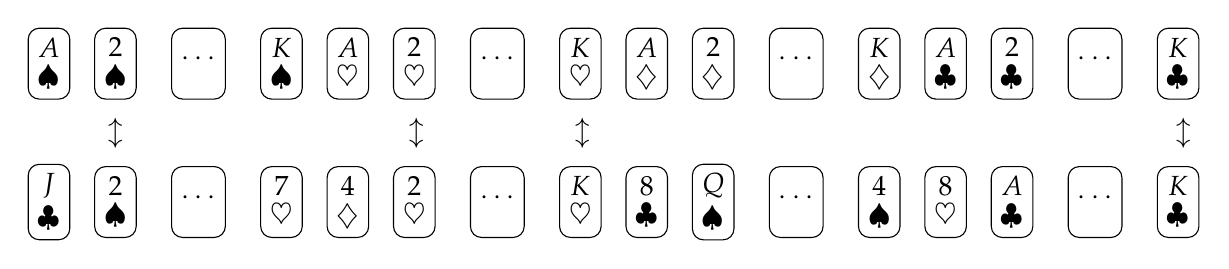
\begin{tikzpicture}
\foreach \x/\v/\s in {
  0/A/\spadesuit,
  1/2/\spadesuit,
  2.25/\cdots/,
  3.5/K/\spadesuit,
  4.5/A/\heartsuit,
  5.5/2/\heartsuit,
  6.75/\cdots/,
  8/K/\heartsuit,
  9/A/\diamondsuit,
  10/2/\diamondsuit,
  11.25/\cdots/,
  12.5/K/\diamondsuit,
  13.5/A/\clubsuit,
  14.5/2/\clubsuit,
  15.75/\cdots/,
  17/K/\clubsuit}
  \node[minimum height=9mm,draw,rounded corners]
    at (\x*24pt,0) {\shortstack{$\v$\\$\s$}};

\foreach \x/\v/\s in {
  0/J/\clubsuit,
  1/2/\spadesuit,
  2.25/\cdots/,
  3.5/7/\heartsuit,
  4.5/4/\diamondsuit,
  5.5/2/\heartsuit,
  6.75/\cdots/,
  8/K/\heartsuit,
  9/8/\clubsuit,
  10/Q/\spadesuit,
  11.25/\cdots/,
  12.5/4/\spadesuit,
  13.5/8/\heartsuit,
  14.5/A/\clubsuit,
  15.75/\cdots/,
  17/K/\clubsuit}
  \node[minimum height=9mm,draw,rounded corners]
    at (\x*24pt,-50pt) {\shortstack{$\v$\\$\s$}};

\node at (24pt,-25pt) {$\updownarrow$};
\node at (133pt,-25pt) {$\updownarrow$};
\node at (193pt,-25pt) {$\updownarrow$};
\node at (410pt,-25pt) {$\updownarrow$};
\end{tikzpicture}
\end{center}
\caption{התאמת שתי חפיסות קלפים}\label{f.cards}
\end{figure}
\solution{}

ההתפלגות אחידה כי לכל קלף בשורה השניה אותה המסתברות להתאים לקלף מעליו. לכן:
\[
E(\textrm{ההתאמות מספר}) = 52\cdot \frac{1}{52} = 1\,.
\]
\selectlanguage{english}
\begin{verbatim}
Expectation of matches = 1.00
Average of matches     = 1.01
\end{verbatim}
\selectlanguage{hebrew}

%%%%%%%%%%%%%%%%%%%%%%%%%%%%%%%%%%%%%%%%%%%%%%%%%%%%%%%%%%%%%%%%

\begin{prob}{הסתברויות של התאמות}{}{(Probabilities of matches)}

סדר חפיסת קלפים בשורה בסדר הסטנדרטי ואז סדר חפיסה שניה שורה בסדר אקראי מתחת לשורה הראשונה (איור%
~\ref{f.cards}).
פתח נוסחה עבור 
$P(n,r)$,
ההסתברות שיהיו בדיוק 
$r$
התאמות של קלף בשורה הראשונה עם קלף בשורה מתחתיו? הנח ש-%
$P(k,0)$
נתון עבור
$0\leq k\leq n$.
\end{prob}
\solution{}

במבט ראשון נראה שבעיה זו דומה לבעיה~28 אבל קיים הבדל מהותי. השליפות המקופסאות הן בלתי-תלויות אבל כאן ההתאמות תלויות אחת בשניה. למשל, אם יש התאמה בקלף הראשון (בהסתברות 
$1/n$),
ההסתברות של התאמה בקלף השני היא
$1/(n-1)$.

ההסתברות שקבוצה 
\textbf{נתונה}
של
$r$
קלפים מתאימות היא:
\begin{equation}\label{eq.r-match}
\disfrac{1}{n}\cdot \disfrac{1}{n-1}\cdot \cdots \cdot \disfrac{1}{n+r-1}\,.
\end{equation}
כדי לקבל בדיוק 
$r$
התאמות, יש להכפיל משוואה%
~\ref{eq.r-match}
ב-%
$P(n-r,0)$,
ההסתברות שאין בכלל התאמות בשאר 
$n-r$
הקלפים. לבסוף, יש 
${n\choose r}$
דרכים לבחור
$r$
התאמות, ולכן:
\begin{eqn}
P(n,r)&=& \dischoose{n}{r}\disfrac{1}{n(n-1)(n+r-1)} P(n-r,0)\\
&=& \disfrac{n!}{r!(n-r)!}\cdot\disfrac{1}{n!/(n-r)!}P(n-r,0)\\
&=&\disfrac{1}{r!}P(n-r,0)\,.
\end{eqn}
נוסחה זו פותרת את הבעיה כי 
$P(k,0)$
נתונה.

\L{Mosteller}
מפתח נוסחה סגורה וגבול עבור
$P(n,r)$:
{
\addtolength{\arraycolsep}{-3pt}
\begin{eqnarray}
P(n,k)&=&\disfrac{1}{k!}\sum_{i=0}^{n-k} \disfrac{(-1)^i}{i!}\\
\label{eq.r-matches-lim}
\lim_{n-r\rightarrow \infty} P(n,k)&\approx& \disfrac{1}{k!}e^{-1}\,.
\end{eqnarray}
}

\textbf{סימולציה}

הרצתי את הסימולציה עבור 
$n=52$
קלפים וחישבתי את ההסתברות ממשוואה%
~\ref{eq.r-matches-lim}.
\selectlanguage{english}
\begin{verbatim}
Probability of 1 matches = 0.3679
Proportion 1 matches     = 0.3710
Probability of 2 matches = 0.1839
Proportion 2 matches     = 0.1828
Probability of 3 matches = 0.0613
Proportion 3 matches     = 0.0569
Probability of 4 matches = 0.0153
Proportion 4 matches     = 0.0168
\end{verbatim}
\selectlanguage{hebrew}

%%%%%%%%%%%%%%%%%%%%%%%%%%%%%%%%%%%%%%%%%%%%%%%%%%%%%%%%%%%%%%%%

\begin{prob}{לבחור את הנדוניה הגדול ביותר}{D}{(Choosing the largest dowry)}

הנח סידרה של 
$n$
קלפים עם הפנים למטה. על פניו של כל קלף נמצא מספר שלם חיובי אבל אין מידע על ההתלפגות שלהם. הפוך את הקלפים אחד-אחד ועיין במספרים. לאחר חשיפת כל אחד מהקלפים, אתה יכול להכריז שמספר זה הוא הגדול ביותר בסידרה. אם אתה צודק אתה מנצח, אחרת אתה מפסיד. למשל, אם הסדרה היא 
$(47, 23, 55, 4)$,
אתה מנצח רק אם אתה בוחר שת הקלף השלישי.

הנה אסטרטגיה: ל-%
$r$
קבוע, וותר על
$r-1$
הקלפים הראשונים ובחר את הקלף הראשון שמספרו גדול מכל 
$r-1$
הקלפים.

\que{1}
עבור
$n=4$
ו-%
$r=3$
בדוק את כל התמורות ומצא בכמה מהם את מנצח.

\que{2}
פתח נוסחה עבור ההסתברות לניצחון עבור 
$n, r$
שרירותיים.

\que{3} מצא קירוב להסתברות כאשר 
$n,r\rightarrow \infty$.

\textbf{רמז:}
נתון
$r$
באיזה מקומות יכול להופיע המספר הגדול ביותר
$m$
ובאיזה מקומות המספרים שהם פחות או שווים ל-%
$m$? 

\end{prob}
\solution{}

\ans{1}
כדי לפשט את הסימון נכתוב את דירוג מספרים כ-%
$1,2,3,4$
למרות שהערכים אמיתיים של המספרים לא ידועים, ולמשל יכולים להיות 
$4,23,47,55$.
אם אתה חושף קלפים
$1,2,3$
(שהם בעצם
$4,23,47$),
אינך יודע אם לבחור
$47$
או לחכות ובחור את הקלף האחרון.

יש 
$24$
תמורות של ארבעה מספרים. לפי האסטרטגיה אתה מוותר על שני הקלפים הראשונים ובוחר או את הקלף השלישי או את הקלף הרביעי, כך שאתה מפסיד אם $4$ נמצא במקום הראשון של התמורה. מה עם התמורה
$(1,2,3,4)$?
אתה מוותר על
$1,2$
ובוחר 
$3$
בגלל שהוא גובהה יותר מ-%
$1,2$
אבל אתה מפסיד כי זה לא המספר הגדולה ביותר. מה עם התמורה
$(1,3,2,4)$?
שוב, לפי האסטרטגיה אתה מוותר על
$1,3$,
אבל מוותר גם על
$2$
כי הוא 
\textbf{לא}
גדול יותר מ-%
$1,3$.
כעת אתה בוחר
$4$
ומנצח. נסח טיעונים דומים לכל התמורות ובדוק שכל התמורות עם 
$4$
במסגרת הן נצחונות:
\[
\addtolength{\arraycolsep}{-2pt}
\renewcommand*{\arraystretch}{1.5}
\begin{array}{cc|cc@{\hspace{2em}}cc|cc@{\hspace{2em}}cc|cc@{\hspace{2em}}cc|cc@{\hspace{2em}}cc|cc@{\hspace{2em}}cc|cc}
1&2\;&\;3&4&
1&2\;&\;\fbox{$4$}&3&
1&3\;&\;2&\fbox{$4$}&
1&3\;&\;\fbox{$4$}&2&
1&4\;&\;2&3&
1&4\;&\;3&2\\
2&1\;&\;3&4&
2&1\;&\;\fbox{$4$}&3&
2&3\;&\;1&\fbox{$4$}&
2&3\;&\;\fbox{$4$}&1&
2&4\;&\;1&3&
2&4\;&\;3&1\\
3&1\;&\;2&\fbox{$4$}&
3&1\;&\;\fbox{$4$}&2&
3&2\;&\;1&\fbox{$4$}&
3&2\;&\;\fbox{$4$}&1&
3&4\;&\;2&1&
3&4\;&\;2&1\\
4&1\;&\;2&3&
4&1\;&\;3&2&
4&2\;&\;1&3&
4&2\;&\;3&1&
4&3\;&\;1&2&
4&3\;&\;2&1
\end{array}
\]
ההסתברות לנצח היא
$10/24$.

\ans{2}
אתה מפסיד אם המספר הגדול ביותר נמצא באחד המקומות
$1,\ldots,r-1$.
לכן כדי לנצח מספר הגדול ביותר חייב להיות במקום
$m$
כאשר
$r\leq m\leq n$:
\[
1\quad 2\quad \cdots\quad r-2 \quad r-1 \quad \overbrace{r \quad r+1 \quad \cdots\quad m-1\quad  m \quad m+1\quad \cdots \quad n}^{\textrm{כאן להיות חייב ביותר גדול מספר}}\,.
\]
לפי האסטרטגיה אתה מוותר על
$r-1$
הקלפים הראשונים. אתה תבחר מקום
$m$
אם ורק אם 
\textbf{כל}
במספרים ב-%
$(r,\ldots,m-1)$
קטנים מ%
\textbf{כל}
המספרים ב-%
$(1,\ldots,r)$.
במילים אחרות, המספר הגדול ביותר בסידרה
$(1,\ldots,m-1)$
הוא
\textbf{לא}
בחלק השני של הסידרה
$(r,\ldots m-1)$
אלא בחלק הראשון
$(1,\ldots,r-1)$.
ההסתברות היא:
\[
P((1,\ldots,r-1)\textrm{ב- נמצא}\;(1,\ldots,m-1)\textrm{ב- ביותר הגדול המספר}) = \disfrac{r-1}{m-1}\,.
\]
ההסתברות שהמספר הגדול ביותר נמצא ב-%
$m$
הוא
$1/n$
ולכן:
\begin{equation}\label{eq.dowry1}
P(\textrm{ניצחון}) = \sum_{m=r}^{n} \disfrac{1}{n} \cdot \disfrac{r-1}{m-1}= \disfrac{r-1}{n}\sum_{m=r}^{n} \disfrac{1}{m-1}\,.
\end{equation}
עבור
$n=4, r=3$, $P(\textrm{ניצחון}) = 5/12=10/24$.

משוואה%
~\ref{eq.dowry1}
לא מוגדרת עבור
$r=1$
אבל ההסתברות לנצח כאשר אתה בוחר את המספר הראשון הוא
$1/n$.
לערך גבוהה ביותר של
$r$
יש הסתברות גבוהה יותר כפי שראינו בדוגמה.

\ans{3}
נכתוב משוואה%
~\ref{eq.dowry1}
כך:
\begin{equation}\label{eq.dowry2}
P(\textrm{ניצחון}) =\disfrac{r-1}{n}\left(\sum_{m=2}^{n} \disfrac{1}{m-1}-\sum_{m=2}^{r-1} \disfrac{1}{m-1}\right)\,.
\end{equation}
עבור 
$n,r$
גדולים, ניתן למצוא קירוב למשוואה%
~\ref{eq.dowry2}
כך:
\[
P(\textrm{ניצחון})=\disfrac{r}{n}(\ln n - \ln r)=\disfrac{r}{n}\ln \disfrac{n}{r}=-\disfrac{r}{n}\ln \disfrac{r}{n}\,.
\]
נסמן
$x=r/n$
ונמצא את המקסימום מהנגזרת:
\begin{eqn}
(-x\ln x)' &=& -x\cdot \frac{1}{x} + (-1) \ln x=0\\
\ln x &=& -1\\
x &=& 1/e\,.
\end{eqn}
כדי למקסם את ההסתברות לנצח בחר
$r \approx n/e$.

\textbf{סימולציה}

הרצתי את הסימולציה עם
$100$
קלפים וערכי
$r$
קרובים ל-%
$100/e$:
\selectlanguage{english}
\begin{verbatim}
Reject cards before r = 36:
Probability of wins   = 0.3674
Proportion wins       = 0.3641
Reject cards before r = 37:
Probability of wins   = 0.3678
Proportion wins       = 0.3759
Reject cards before r = 38:
Probability of wins   = 0.3679
Proportion wins       = 0.3548
Reject cards before r = 30:
Probability of wins   = 0.3590
Proportion wins       = 0.3601
\end{verbatim}
\selectlanguage{hebrew}

%%%%%%%%%%%%%%%%%%%%%%%%%%%%%%%%%%%%%%%%%%%%%%%%%%%%%%%%%%%%%%%%

\begin{prob}{בחירת המספר האקראי הגדול ביותר}{D}{(Choosing the largest random number)}

הנח סידרה של 
$n$
קלפים עם הפנים למטה. על פניו של כל קלף נמצא מספר ממשי עם התפלגות אחידה ב-%
$0.0\leq x<1.0$.
הפוך את הקלפים אחד-אחד ועיין במספרים. לאחר חשיפת כל אחד מהקלפים, אתה יכול להכריז שמספר זה הוא הגדול ביותר בסידרה. אם אתה צודק אתה מנצח, אחרת אתה מפסיד.

השתמש באסטרטגיה של בעיה~37: החלט על ערך
$r$
כך שאתה מוותר על 
$r-1$
הקלפים הראשונים ובוחר את הקלף הראשון שגדול מהמספר הגדול ביותר ב-%
$r-1$
קלפים הראשונים.

\textbf{הגדרה:}
$d$,
\textbf{ערך שווה-נפש},
הוא הערך שמתחתיו אתה מוותר על הקלף ומעליו את לבחור את הקלף.

\que{1} 
חשב את
$d$
עבור
$n=1$
וחשב את ההסתברות לנצח.

\que{2}
חשב את
$d$
עבור
$n=2$
וחשב את ההסתברות לנצח.

\que{3}
חשב את
$d$
עבור
$n=3$.
אל תנסה לחשב את ההסתברות לנצח!

\textbf{הערה:}
בבעיה~37 בערכים יכולים להיות
$100, 200, 300$ 
או
$100, 50, 20$
כך שחשיפת המספר הראשון לא מספק שום מידע על המספרים האחרים. בבעיה זו, ההתלפגות אחידה, ולכן אם המספר הראשון הוא 
$0.2$,
ההסתברות שהמספר השני יהיה גדול יותר היא 
$0.8$
ואם המספר הראשון הוא 
$0.8$
ההסתברות שהמספר השני יהיה גדול יותר היא
$0.2$.

\end{prob}
\solution{}

יהי
$v_1,v_2,v_3$
המספרים על שלושת הכרטיסים.

\ans{1}
אין ברירה אלא לבחור את הקלף הראשון כי אין קלפים אחרים. לכן אין ערך שווה-נפש. 
$v_1$
הוא המספר "הגדול ביותר",
$P(\textrm{ניצחון})=1$.

\ans{2}
אם אתה בוחר את הקלף הראשון
$P(\textrm{ניצחון})=v_1$
שהיא ההסתברות שהמספר על הקלף השני קטן יותר. אם אתה מוותר על הקלף הראשון,
$P(\textrm{ניצחון})=1-v_1$
שהיא ההסתברות ש-%
$v_2>v_1$.
לכן, אם 
$v_1<0.5$ 
בחר את הקלף השני כי
$1-v_1>0.5$
ואם 
$v_1>0.5$
בחר את הקלף הראשון. מכאן ש-%
$d=0.5$.

הנה הנוסחה לחישוב ההסתברות לנצח:
\[
P(\textrm{ניצחון}) = p(\textrm{ניצחון} \,|\,v_1<0.5)\,p(v_1<0.5)+ p(\textrm{ניצחון}\,|\,v_1>0.5)\,p(v_1>0.5)\,.
\]
$p(v_1<0.5)=0.5$
נובע מההתפלגות האחידה. מה עם
$p(\textrm{ניצחון} \,|\,v_1<0.5)$? 
לפי האסטרטגיה אתה מנצח אם
$0.5<v_2<1$
אבל גם אם
$v_1<v_2<0.5$.
ההתפלגות של 
$v_1$
היא אחידה ב-%
$(0,0.5)$
ולכן:
\[
p(\textrm{ניצחון} \,|\,v_1<0.5)=\disfrac{1}{2} + \disfrac{1}{4}=\disfrac{3}{4}\,.
\]
ניתן לעשות חישוב דומה עבור
$v_1>0.5$.
נרכיב את כל החישובים הללו ביחד וקבל:
\[
P(\textrm{ניצחון})=\disfrac{3}{4}\cdot\disfrac{1}{2}+\disfrac{3}{4}\cdot\disfrac{1}{2}=\disfrac{3}{4}\,.
\]

\ans{3}
אם אתה בוחר את הקלף הראשון,
$P(\textrm{ניצחון})=v_1^2$
כי הקלף השני והשלישי חייבים להיות קטנים מהראשון.

אם אתה מוותר על הקלף הראשון ובוחר את השני כי 
$v_2>v_1$
אזי:
\begin{itemize}
\item $P(\textrm{ניצחון})=(1-v_1)v_1$
אם
$v_2>v_1$ 
ו-%
$v_3<v_1$.
\item $P(\textrm{ניצחון})=v_1(1-v_1)$
אם
$v_2<v_1$
ו-%
$v_3>v_1$.
\item $P(\textrm{ניצחון})=\frac{1}{2}(1-v_1)^2$
אם
$v_2>v_1$
ו-%
$v_3>v_1$,
כי ניצחון תלוי בסדר:
\\
אם הוא
$(0.55, 0.75, 0.65)$
אתה מנצח
ואם הוא
$(0.55, 0.65, 0.75)$
אתה מפסיד.
\end{itemize}

הערך שווה-נפש 
$d$
הוא ערך עבורו ההסתברות לנצח על ידי בחירת הקלף הראשון שווה להסתברות לנצח על ידי ויתור על הקלף הראשון:
\begin{eqn}
d^2 &=& 2d(1-d) + \frac{1}{2}(1-d)^2\\
5d^2 - 2d -1 &=&0\\
d&=& \disfrac{1+\sqrt{6}}{5}\approx 0.6899\,.
\end{eqn}
\L{Gilbert\&Mosteller \cite[page~55]{gilbert}}
מראים שעבור
$n=3$:
\[
P(\textrm{ניצחון}) = \disfrac{1}{3}+\disfrac{d}{2}+\disfrac{d^2}{1}-\disfrac{3d^3}{2}\approx 0.6617\,.
\]
\textbf{סימולציה}
\selectlanguage{english}
\begin{verbatim}
For  3 cards:
Indifference value = 0.6000
Probability of win = 0.6693
Proportion of wins = 0.6628
Indifference value = 0.6899
Probability of win = 0.6617
Proportion of wins = 0.6711
Indifference value = 0.7200
Probability of win = 0.6519
Proportion of wins = 0.6473
\end{verbatim}
\selectlanguage{hebrew}

%%%%%%%%%%%%%%%%%%%%%%%%%%%%%%%%%%%%%%%%%%%%%%%%%%%%%%%%%%%%%%%%

\begin{prob}{להכפיל את הדיוק}{}{(Doubling your accuracy)}

נתון שני מקלות באורכים
$L_1<L_2$
ומכשיר למדידת מרחק ששגיאת המדידה שלו ניתן על ידי התפלגות נורמלית עם ממוצע
$0$
ושונות
$\sigma^2$.
ניתן למדוד את אורכי המקלות על ידי מדידת כל מקל בנפרד. האם יש דרך מדוייקת יותר?
\end{prob}
\solution{}

\begin{figure}[bt]
\begin{center}
\begin{tikzpicture}
\draw (0,0) -- ++(6,0) -- ++(0,12pt) -- ++(-6,0) -- cycle;
\draw[<->] (0,24pt) --
  node[fill=white] {$\scriptstyle L_1+L_2$} ++(14,0);
\draw (6,0) -- ++(8,0) -- ++(0,12pt) -- ++(-8,0) -- cycle;
\begin{scope}[yshift=-48pt]
\draw (0,0) -- ++(8,0) -- ++(0,12pt) -- ++(-8,0) -- cycle;
\draw[yshift=12pt] (0,0) -- ++(0,12pt) -- ++(6,0) -- ++(0,-12pt);
\draw[<->] (6,20pt) --
  node[fill=white] {$\scriptstyle L_2-L_1$} ++(2,0);
\end{scope}
\end{tikzpicture}
\end{center}
\caption{מדידת האורכים של שני מקלות}\label{f.rods}
\end{figure}
הנח את המקלות קצה לקצה ומדד
$L_s=L_1+L_2$,
ואחר כך הנח את המקלות צד לצד ומדד
$L_d=L_2-L_1$ (איור%
~\ref{f.rods}).
חשב
$L_1,L_2$:
\begin{eqn}
\textstyle\frac{1}{2}(L_s-L_d)=\frac{1}{2}((L_1+L_2)-(L_2-L_1))&=&L_1\\
\textstyle\frac{1}{2}(L_s+L_d)=\frac{1}{2}((L_1+L_2)+(L_2-L_1))&=&L_2\,.
\end{eqn}
השגיאות במדידות הן
$e_s, e_d$
כך שהשגיאות התוצאות הן:
\begin{eqn}
\textstyle\frac{1}{2}((L_s+e_s)-(L_d+e_d))&=&L_1+\textstyle\frac{1}{2}(e_s-e_d)\\
\textstyle\frac{1}{2}((L_s+e_s)+(L_d+e_d))&=&L_2+\textstyle\frac{1}{2}(e_s+e_d)\,.
\end{eqn}
ממוצע של השגיאות במכשיר הוא
$0$
ולכן הממוצע של שתי המדידות גם כן $0$. השונות יורדת למחצית ערכה הקודמת:%
\footnote{%
המדידות בלתי-תלויות ולכן הקווריאנס הוא $0$.}
\begin{eqn}
\mathrm{Var}\left(\textstyle\frac{1}{2}\left(e_s-e_d\right)\right)&=&
  \textstyle\frac{1}{4}(\sigma^2+(-1)^2\sigma^2)=\frac{1}{2}\sigma^2\\
\mathrm{Var}\left(\textstyle\frac{1}{2}(e_s+e_d)\right)&=&
  \textstyle\frac{1}{4}( \sigma^2+\sigma^2)=\frac{1}{2}\sigma^2\,.
\end{eqn}


%%%%%%%%%%%%%%%%%%%%%%%%%%%%%%%%%%%%%%%%%%%%%%%%%%%%%%%%%%%%%%%%

\begin{prob}{משוואות ריבועיות אקראיות}{}{(Random quadratic equations)}

תהי 
$x^2+2bx+c=0$
משוואה ריבועית המוגדרת מעל
$[-B,B]\times[-B,B]$
עבור
$B\geq 1$.

\que{1}
מה ההסתברות שהשורשים ממשיים?

\que{2} 
כאשר 
$B\rightarrow \infty$
מה ההסתברות שהשורשים ממשיים?
\end{prob}
\solution{}

\ans{1}
השורשים יהיו ממשיים אם הדיסקרימיננט 
$4b^2-4c\geq 0$
לא-שלילי. איור%
~\ref{f.real-roots}
מראה גרף של הפרבולה
$c=b^2$
כאשר השורשים המרוכבים נמצא בשטח האפור. למשל, עבור
$(b,c)=(1,2)$, 
ל-%
$x^2+2x+2$
שורשים מרוכבים (נקודה אדומה) ועבור
$(b,c)=(2,2)$
ל-%
$x^2+4x+2$
שורשים ממשיים (נקודה כחולה).

\begin{figure}[tb]
\begin{center}
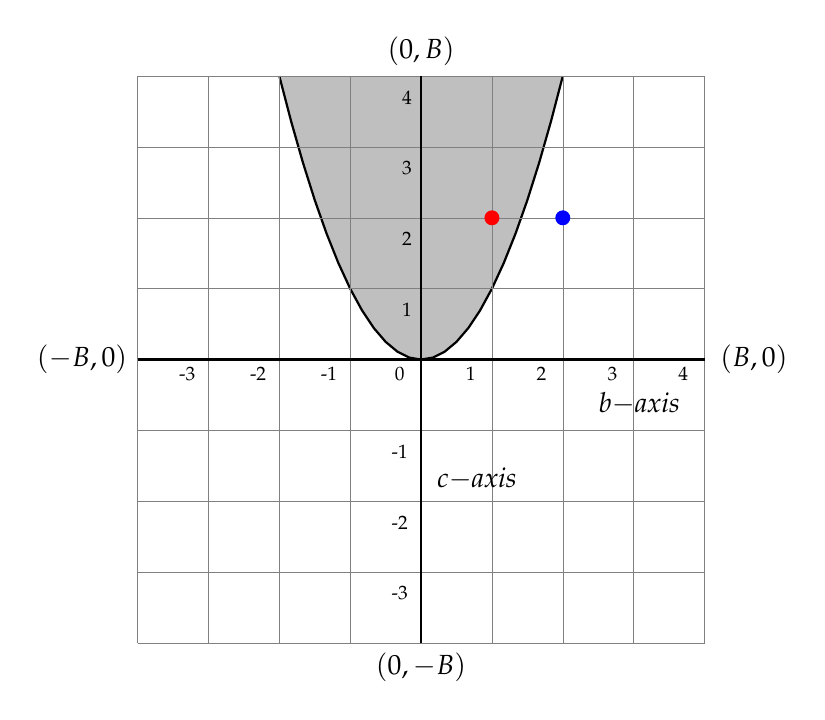
\begin{tikzpicture}[scale=.9]
\fill [white!50!gray, domain=-2:2]
      (-2, 4) -- plot ({\x}, {\x*\x}) -- (2, 4) -- cycle;
\draw [thick, domain=-2:2]
      (-2, 4) -- plot ({\x}, {\x*\x}) -- (2, 4);
\draw[help lines] (-4,-4) grid (4,4);
\draw[thick] (-4,0) -- (4,0);
\draw[thick] (0,-4) -- (0,4);
\foreach \x in {-3,...,4}
  \node at (\x-.3,-.2) {\scriptsize \x};
\foreach \y in {1,...,4}
  \node at (-.2,\y-.3) {\scriptsize \y};
\foreach \y in {-3,...,-1}
  \node at (-.3,\y-.3) {\scriptsize \y};
\draw[thick] (0,-4) node[below] {$(0,-B)$} -- 
  node[right,near start,xshift=2pt,yshift=8pt]
  {$c\mathit{-axis}$} (0,4) node[above] {$(0,B)$};
\draw[thick] (-4,0) node[left] {$(-B,0)$} --
  node[below,very near end,xshift=2pt,yshift=-8pt] 
  {$b\mathit{-axis}$} (4,0) node[right,xshift=2pt] {$(B,0)$};
\fill[red] (1,2) circle(3pt);
\fill[blue] (2,2) circle(3pt);
\end{tikzpicture}
\end{center}
\caption{%
עבור 
$(b,c)$
בשטח האפור השורשים של
$c=b^2$
מרוכבים}
\label{f.real-roots}
\end{figure}

נחשב את השטח האפור על ידי אינטגרציה:
\[
\int_{-\sqrt{B}}^{\sqrt{B}} (B-b^2)\,db=
\left. Bb-\disfrac{b^3}{3}\right|_{-\sqrt{B}}^{\sqrt{B}}=
\left(B^{3/2}-\frac{B^{3/2}}{3}\right)-
\left(-B^{3/2}+\frac{B^{3/2}}{3}\right)=
\disfrac{4}{3}B^{3/2}\,.
\]
השטח הכולל של
$[-B,B]\times[-B,B]$
הוא
$4B^2$
ולכן:
\begin{eqn}
P(\textrm{מרוכבים שורשים})&=&\disfrac{\frac{4}{3}B^{3/2}}{4B^2}=\disfrac{1}{3\sqrt{B}}\\
P(\textrm{ממשיים שורשים})&=&1-\disfrac{1}{3\sqrt{B}}\,.
\end{eqn}
\ans{2}
\[
\lim_{B\rightarrow\infty}
P(\textrm{ממשיים שורשים})=
\lim_{B\rightarrow\infty} \left(1-\disfrac{1}{3\sqrt{B}}\right)=
1\,.
\]

\textbf{סימולציה}
\selectlanguage{english}
\begin{verbatim}
For B =  4:
Probability of real roots = 0.8333
Proportion real roots     = 0.8271
For B = 16:
Probability of real roots = 0.9167
Proportion real roots     = 0.9205
For B = 64:
Probability of real roots = 0.9583
Proportion real roots     = 0.9582
\end{verbatim}
\selectlanguage{hebrew}

%%%%%%%%%%%%%%%%%%%%%%%%%%%%%%%%%%%%%%%%%%%%%%%%%%%%%%%%%%%%%%%%

\begin{prob}{הילוך מקרי דו-ממדי}{}{(Two-dimensional random walk)}

חלקיק נמצא במרכז של מערכת צירים דו-ממדית. החלקיק צועד ימינה או שמאלה על ציר ה-%
$x$
עם הסתברות 
$1/2$
לכל כיוון 
\textbf{ובו-זמנית}
צועד למעלה או למטה על ציר ה-%
$y$
עם הסתברות 
$1/2$
לכל כיוון. איור%
~\ref{f.2d-random-walk}
מראה הילוך מקרי של 
$22$
צעדים שמתחיל ונגמר במרכז.

\que{1}
מה ההסתברות שהחלקיק חוזר למרכז ב-$2$ צעדים?

\que{2}
פתח נוסחה עבור ההתסתברות שהחלקיק חוזר למרכז (פעם אחת או יותר).

\que{3}
השתמש בקירוב של
\L{Stirling}
כדי לקבל הערכה של ההסתברות עבור $n$ גדול.

\begin{figure}[t]
\begin{center}
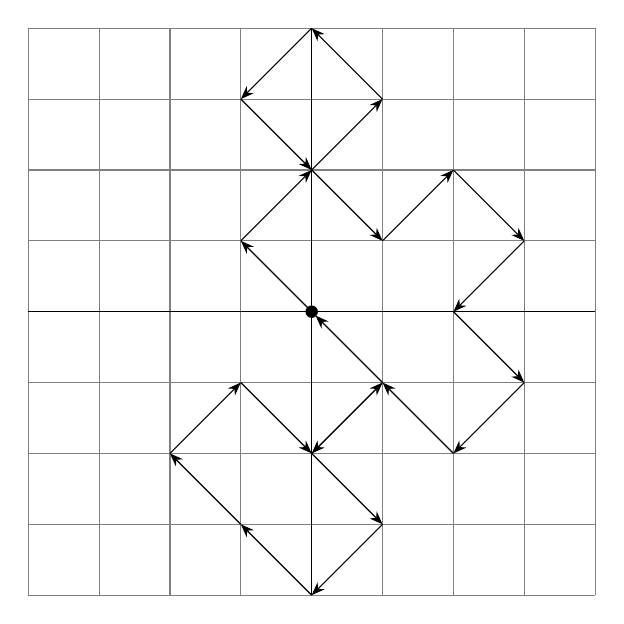
\begin{tikzpicture}[scale=.9]
\draw[color=gray] (-4,-4) grid (4,4);
\draw (-4,0) -- (4,0);
\draw (0,-4) -- (0,4);
\fill (0,0) circle[radius=2.5pt];
\draw[->] (0,0)  -- (-1,1);
\draw[->] (-1,1) -- (0,2);
\draw[->] (0,2)  -- (1,3);
\draw[->] (1,3)  -- (0,4);
\draw[->] (0,4)  -- (-1,3);
\draw[->] (-1,3) -- (0,2);
\draw[->] (0,2)  -- (1,1);
\draw[->] (1,1)  -- (2,2);
\draw[->] (2,2)  -- (3,1);
\draw[->] (3,1)  -- (2,0);
\draw[->] (2,0)  -- (3,-1);
\draw[->] (3,-1) -- (2,-2);
\draw[->] (2,-2) -- (1,-1);
\draw[->] (1,-1) -- (0,-2);
\draw[->] (0,-2) -- (1,-3);
\draw[->] (1,-3) -- (0,-4);
\draw[->] (0,-4) -- (-1,-3);
\draw[->] (-1,-3)-- (-2,-2);
\draw[->] (-2,-2)-- (-1,-1);
\draw[->] (-1,-1)-- (0,-2);
\draw[->] (0,-2) -- (1,-1);
\draw[->] (1,-1) -- (.055,-.055);
\end{tikzpicture}
\end{center}
\caption{הילוך מקרי דו-ממדי}\label{f.2d-random-walk}
\end{figure}
\end{prob}
\solution{}

\ans{1}
הנקודות באיור%
~\ref{f.two-moves}
מראות את המקומות האפשריים בהם החלקיק יכול להיות לאחר שני צעדים:
\begin{itemize}
\item
המסלול הירוק מראה איך להגיע ל-%
$(\pm 2, \pm 2)$
על ידי שני צעדים באותו כיוון. ההסתברות היא
$\left(\frac{1}{4}\right)^2= \frac{1}{16}$.
\item
המסלול האדום מראה איך להגיע ל-%
$(\pm 2,0)$
או ל-%
$(0,\pm 2$).
יש שני מסלולים אפשריים לכל נקודה ולכן ההסתברות היא
$2\cdot\left(\frac{1}{4}\right)^2= \frac{2}{16}$.
\item
המסלול הכחול מראה איך להגיע ל-%
$(\pm 1,\pm 1)$
ולחזור למרכז. ההסבתרות היא
$1/16$.
יש ארבעה מסלולים שחוזרים למרכז ולכן ההסתברות היא
$\frac{4}{16}$.
\end{itemize}
רק המסלולים הכחולים חוזרים למרכז ולכן:
\[
P(\textrm{צעדים בשני למרכז חזרה})=\frac{4}{16}\,.
\]

\begin{figure}[tb]
\begin{center}
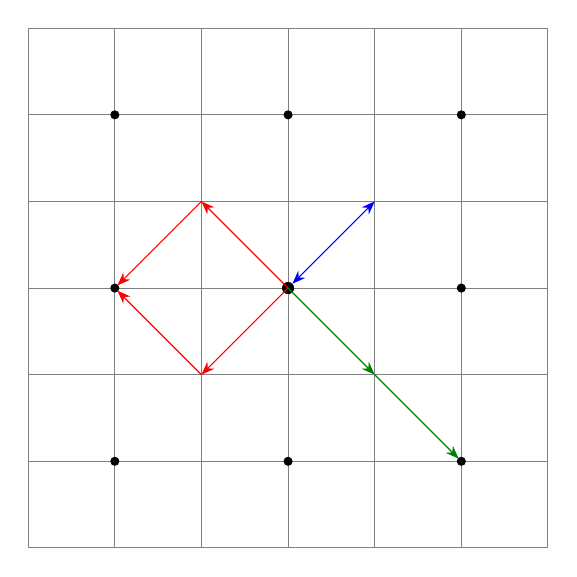
\begin{tikzpicture}[scale=1.1]
\draw[color=gray] (-3,-3) grid (3,3);
\fill (0,0) circle[radius=2pt];
\foreach \x/\y in {2/2, 2/-2, -2/2, -2/-2, 
                   0/2, 0/-2, 2/0, -2/0}
  \fill (\x,\y) circle[radius=1.5pt];
\draw[->,red] (0,0) -- (-1,-1);
\draw[->,red] (-1,-1) -- (-1.97,-.03);
\draw[<-,red] (-1.97,0.03) -- (-1,1);
\draw[<-,red] (-1,1) -- (0,0);
\draw[->,green!50!black] (0,0) -- (1,-1);
\draw[->,green!50!black] (1,-1) -- (1.97,-1.97);
\draw[<->,blue] (.05,.05) -- +(.95,.95);
%\draw[->,blue] (-0.1,0) -- +(1,1);
%\draw[->,blue] (1.1,1) -- +(-1,-1);
\end{tikzpicture}
\end{center}
\caption{שני צעדים בהילוך מקרי}\label{f.two-moves}
\end{figure}

\ans{3}
בחירת הכיוון בשני מצירים היא בלתי-תלויה כך שעבור
$2n$
צעדים:
\begin{equation}\label{eq.2d-1}
P_{2n}(\textrm{למרכז חזרה}) =
P_{2n}(x\!=\!0\textrm{ל- חזרה})\,P_{2n}(y\!=\!0\textrm{ל- חזרה})\,.
\end{equation}
החלקיק יחזור למרכז אם ורק אם בשני הצירים מספר הצעדים 
$+1$
שווה המספר צעדים
$-1$.
יש 
${2n \choose n}$
דרכים לסדר
$+1$
ו-%
$-1$
ולכן:
{
\addtolength{\arraycolsep}{-3pt}
\begin{eqnarray}
P_{2n}(x\!=\!0\textrm{ל- חזרה}) =P_{2n}(y\!=\!0\textrm{ל- חזרה})&=&
\dischoose{2n}{n}\left(\disfrac{1}{2}\right)^n\left(\disfrac{1}{2}\right)^{n}\\
P_{2n}(\textrm{למרכז חזרה}) &=&
\left[\dischoose{2n}{n}\left(\disfrac{1}{2}\right)^{2n}\right]^2\\
P(\textrm{למרכז חזרה}) =
\sum_{n=1}^{\infty}P_{2n}(\textrm{למרכז חזרה}) &=&
\sum_{n=1}^{\infty}\left[\dischoose{2n}{n}\left(\disfrac{1}{2}\right)^{2n}\right]^2\,.\label{eq.2d-2}
\end{eqnarray}
}
\ans{3}
לפי הקירוב של
\L{Stirling}
$n! \approx \sqrt{2\pi n}\left(n/e\right)^n$:
\begin{eqn}
P_{2n}(\textrm{למרכז חזרה}) &=&
\left[\dischoose{2n}{n}
\left(\disfrac{1}{2}\right)^{2n}\right]^2 \\
&=&
\left[\disfrac{(2n)!}{(n!)^2}
\left(\disfrac{1}{2}\right)^{2n}\right]^2 \\
&\approx&
\left(\disfrac{1}{2}\right)^{4n}
\disfrac{(\sqrt{2\pi \cdot 2n})^2
         \left(2n/e\right)^{4n}}
        {(\sqrt{2\pi n})^{4}
         \left(n/e\right)^{4n}} \\
&=&\left(\disfrac{1}{2}\right)^{4n}\disfrac{4\pi n}{4\pi^2 n^2}\cdot
\disfrac{\left(n/e\right)^{4n}\cdot 2^{4n}}{\left(n/e\right)^{4n}}\\
&=& \disfrac{1}{\pi n}\\
P(\textrm{למרכז חזרה}) &=& \disfrac{1}{\pi}\sum_{n=1}^{\infty}\disfrac{1}{n}\,,
\end{eqn}
שהיא
\textbf{סידרה הרמונית}
שמתבדרת, כלומר, עם הסתברות 
$1$
החלקיק חוזר למרכז!

\textbf{סימולציה}
הרצתי את הסימולציה מיליון פעמים במקום עשרת אלפים פעמים אבל התוצאה לא מראה שהחלקיק מגיע למרכז בוואדות.
\selectlanguage{english}
\begin{verbatim}
Proportion returned to origin      = 0.8700
\end{verbatim}
\selectlanguage{hebrew}

%%%%%%%%%%%%%%%%%%%%%%%%%%%%%%%%%%%%%%%%%%%%%%%%%%%%%%%%%%%%%%%%

\begin{prob}{הילוך מקרי תלת-ממדי}{D}{(Three-dimensional random walk)}

לקיק נמצא במרכז של מערכת צירים תלת-ממדית. החלקיק צועד ימינה או שמאלה על ציר ה-%
$x$
עם הסתברות 
$1/2$
לכל כיוון 
\textbf{ובו-זמנית}
צועד למעלה או למטה על ציר ה-%
$y$
עם הסתברות 
$1/2$
לכל כיוון.
\textbf{ובו-זמנית}
צועד פנימה או החוצה על ציר ה-%
$z$
עם הסתברות 
$1/2$
לכל כיוון.

\que{1}
מה
\textbf{התוחלת}
של מספר הפעמים שהחלקיק חוזר למרכז?

\textbf{רמז:}
חשב את ההסתברות ואחר כך תשתמש במשתנה מסמן
\L{(indicator variable)}.

\que{2}
מה ההסתברות שהחלקיק יחזור למרכז לפחות פעם אחת?

\textbf{רמז:}
תשתשמש בשיטה של בעיה~4.
\end{prob}
\solution{}

$P_{2n}$,
ההסתברות לחזור למרכז לאחר
$2n$
נתון על ידי הכללת משוואה%
~\ref{eq.2d-1}
לשלושה ממדים:
\[
P_{2n} =
P_{2n}(x=0\textrm{ל- חוזר})\,P_{2n}(y=0\textrm{ל- חוזר}\, P_{2n}(z=0\textrm{ל- חוזר})\,.
\]
$P_r$,
ההסתברות לחזור למרכז לפחות פעם אחת ניתנת על ידי הכללה לשלושה ממדים של משוואה%
~\ref{eq.2d-2}:
\[
P_r =\sum_{n=1}^{\infty}P_{2n} =
\sum_{n=1}^{\infty}\left[\dischoose{2n}{n}\left(\disfrac{1}{2}\right)^{2n}\right]^3\,.
\]
מהקירוב של
\L{Stirling}:\footnote{\L{Mosteller}
השתמש ב-%
$18$
איברים בחישוב שלו וקיבל
$0.315$.
התכנית שלי השתמש ב-%
$500$
איברים וקיבלתי
$0.3772$.}
\begin{eqn}
P_{2n} &=&
\left[\disfrac{(2n)!}{(n!)^2}
\left(\disfrac{1}{2}\right)^{2n}\right]^3 \\
&\approx&
\left(\disfrac{1}{2}\right)^{6n}
\disfrac{(\sqrt{2\pi \cdot 2n})^3
         \left(2n/e\right)^{6n}}
        {(\sqrt{2\pi n})^{6}
         \left(n/e\right)^{6n}} \\
&=&\disfrac{(4\pi n)^{3/2}}{(2\pi n)^3}=
 \disfrac{1}{(\pi n)^{3/2}}\\
P_r &=& \sum_{n=1}^{\infty}\disfrac{1}{(\pi n)^{3/2}}\approx 0.3772\,.
\end{eqn}
יהי 
$I_k$
משתנה מסמן עבור חזרה למרכז בצעד
$k$:
\begin{equation}
I_k=
\left\{
\begin{array}{ll}
1,\quad k\;\textrm{בצעד למרכז חוזר החלקיק אם}\\
0, \quad k\;\textrm{בצעד למרכז חוזר לא החלקיק אם}\,.
\end{array}
\right.
\end{equation}
אזי:
\[
E(\textrm{למרכז החזרות מספר})=\sum_{n=1}^{\infty}P_{2n}\, I_{2n} = P_r\approx 0.3772\,,
\]
ולכן התוחלת למספר החזרות למרכז שווה להסתברות.

\que{2}
תהי
$P_1$
ההסתברות שהחלקיק חוזר למרכז
\textbf{לפחות פעם אחת}.
מבעיה~4 אנו יודעים שהתוחלת של מספר בניסויים עד מראשון בו החלקיק 
\textbf{לא}
חוזר למרכז היא
$1/(1-P_1)$.
לכן, התוחלת של מספר הניסויים עד שהחליק כן חוזר למרכז היא אחד פחות, כי החלקיק יכול לחזור למרכז מספר רב של פעמים עד שהוא לא חוזר.%
\footnote{%
קשה לעקוב אחר הצגת הדברים של
\L{Mosteller}.
ברצוני להודית ל-%
\L{Aaron Montgomery}
שהבהיר לי את הפתרון
\L{\cite{montgomery}}.}

תהי
$E_r=E(\textrm{למרכז החזרות מספר})$. 
אזי:
\begin{eqn}
E_r &=& \disfrac{1}{1-P_1} - 1\\
P_1&=& \disfrac{E_r}{1+E_r}\,.
\end{eqn}
ב-%
\ansnc{1}
חישבנו ש-%
$E_r\approx 0.3772$
ולכן:
\[
P_1 \approx 1- \disfrac{1}{1+0.3772}
\approx 0.2739\,.
\]

\textbf{סימולציה}
\selectlanguage{english}
\begin{verbatim}
Expectation of reaching origin = 0.3772
Average times reached origin   = 0.3630
Probability of reaching origin = 0.2739
Proportion reached origin      = 0.2790
\end{verbatim}
\selectlanguage{hebrew}

%%%%%%%%%%%%%%%%%%%%%%%%%%%%%%%%%%%%%%%%%%%%%%%%%%%%%%%%%%%%%%%%

\begin{prob}{המחט של \L{Buffon}}{D}{(Buffon's needle)}

נתון משטח עם קווים מקביליים במרחק 
$1$
אחד מהשני. קח מחט באורך 
$a\leq 1$
וזרוק אותו על המשטח. מה ההסתברות שהמחט חוצה קו?%
\footnote{%
כדי להקל על החישובים אנו מניחים שהמרחק בין הקווים הוא 
$1$.
ניתן להתעלם מאפשרות שהמחט שוכב כולו לאורך אחד הקווים וכן את האפשרות שהוא נודע בשני קווים כי ההתסברות של אירועים אלה היא אפס.}

\textbf{רמז:}
יש שני משתנים אקראיים (איור%
~\ref{f.buffon1}): 
$x$,
המקום של מרכז המחט ביחס לקו הקרוב ביותר עם התפלגות אחידה בטווח 
$[0,1/2]$,
ו-%
$\theta$, 
הזווית שבין המחט לבין הקווים המקביליים עם התפלגות אחידה בטווח 
$[0,\pi/2]$.

\begin{figure}[tb]
\begin{center}
\begin{tikzpicture}[scale=.9]
\draw (0,0) -- (10,0);
\draw (0,4) -- (10,4);
\draw[<->] (1,0) -- node[fill=white] {$1$} (1,4);
\coordinate (center) at ($(4,-.5)+(60:1.5)$);
\node[above right,xshift=4pt] at (center) {$\theta$};
\node[above left] at (center) {$C$};
\draw[thick] (4,-.5) -- node[right,very near end] {$a$} +(60:4);
\draw[thick,dashed] ($(center)+(-2,0)$) -- +(6,0);
\draw[<->] (5.3,0) -- node[fill=white] {$x$}
  (center -| 5.3,0);
\end{tikzpicture}
\end{center}
\caption{המחט של\;Buffon}\label{f.buffon1}
\end{figure}
\end{prob}
\solution{1}

תהי 
$p(a)$
ההסתברות שמחט באורך 
$a$
חוצה קו והגדר משתנה מסמן:
\[
I_{\textrm{קו חוצה}}=
\left\{
\begin{array}{ll}
1,\quad \textrm{קו חוצה}\;a\;\textrm{באורך מחט}\\
0,\quad \textrm{קו לא חוצה}\;a\;\textrm{באורך מחט}\,.
\end{array}
\right.
\]
אזי:
\begin{equation}\label{eq.buffon-probability}
E(I_{\textrm{קו חוצה}})=1\cdot p(a) + 0\cdot (1-p(a))=p(a)\,,
\end{equation}
וניתן לחשב את ההסתברות על ידי חישוב התוחלת.

יהי 
$m$
אנח לקווים המקביליים שעובר דרך מרכז המחט ותהי 
$\theta$
הזווית בין המחט לבין אחד מהקווים המקביליים. הטל את המחט על 
$m$
כדי לקבל את הקטע הקו
$\overline{CD}$
(איור%
~\ref{f.buffon2}).
ההסתברות שהמחט חוצה קו היא:
\begin{equation}\label{eq.cross}
P(\textrm{קו חוצה}\;\theta\;\textrm{וזווית}\;a\;\textrm{באורך מחט})=\disfrac{(a/2)\sin \theta}{1/2}=a\sin\theta\,.
\end{equation}

\begin{figure}[bt]
\begin{center}
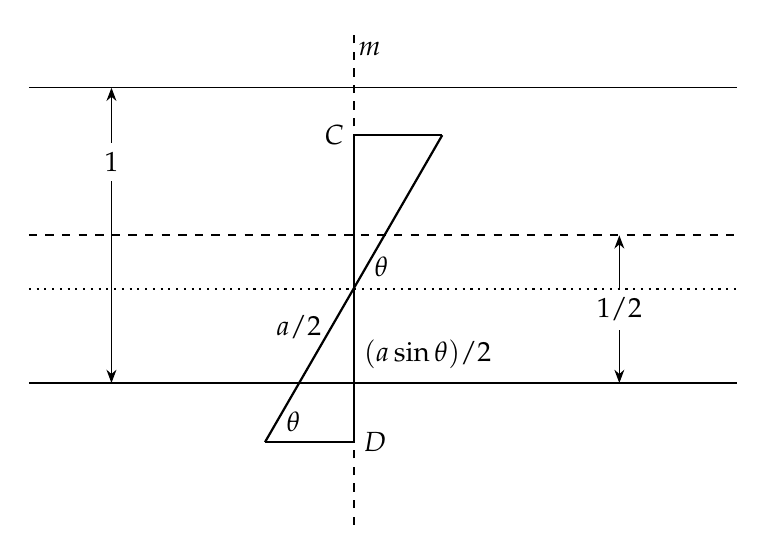
\begin{tikzpicture}[scale=1.5]
\draw (0,0) coordinate (O) -- (6,0);
\draw (0,2.5) -- (6,2.5);
\draw[<->] (.7,0) -- node[fill=white,near end] {$1$} +(0,2.5);
\draw[<->] (5,0) -- node[fill=white] {$1/2$} +(0,1.25);
\coordinate (end1) at (2,-.5);
\coordinate (end2) at ($(end1)+(60:3)$);
\coordinate (center) at ($(end1)+(60:1.5)$);
\draw[thick,dotted] (O |- center) -- +(6,0);
\draw[thick,dashed] (0,1.25) -- +(6,0);
\node[right,xshift=4pt,yshift=8pt]
  at (center) {$\theta$};
%\node[left,xshift=-4pt,yshift=-8pt]
%  at (center) {$\theta$};
\draw[thick,dashed] ($(center)+(0,-2)$) --
  node[right,very near end,xshift=-2pt,yshift=15pt]
  {$m$} +(0,4.2);
\node[right] at (end1 -| center) {$D$};
\node[left] at (end2-| center) {$C$};
\draw[thick] (end1) -- 
  node[left,near end] {$a/2$} (center) --
%  node[right] {$a/2$} 
  (end2);
\draw[thick] (end1) node[above right,xshift=4pt] {$\theta$} --
  (end1 -| center) --
  node[right,yshift=4pt] {$(a\sin\theta)/2$} (center);
\draw[thick] (end2) -- (end2 -| center) -- (center);
%\draw[thick] (end2) node[below left,xshift=-4pt] {$\theta$} --
%  (end2 -| center) -- 
%  node[left] {$(a\sin \theta)/2$} (center);
\end{tikzpicture}
\end{center}
\caption{משולש ישר-זווית לפתרון בעיית המחט של \L{Buffon}}
\label{f.buffon2}
\end{figure}

התוחלת של מספר הקווים שהמחט חוצה מתקבלת על ידי אינטגרציה מעל לזוויות האפשריות:
\begin{equation}\label{eq.buffon-integral}
E(\textrm{lines crossed}) =
  \disfrac{1}{(\pi/2)-0} \int_0^{\pi/2} a\sin \theta\,
  d\theta=\left.\disfrac{2}{\pi}\cdot a (-\cos \theta)
  \right|_0^{\pi/2}=\disfrac{2a}{\pi}\,.
\end{equation}

\solution{2}
הפתרון מבוסס על
\L{\cite[Chapter~26]{proofs}}.

\begin{figure}[tb]
\begin{center}
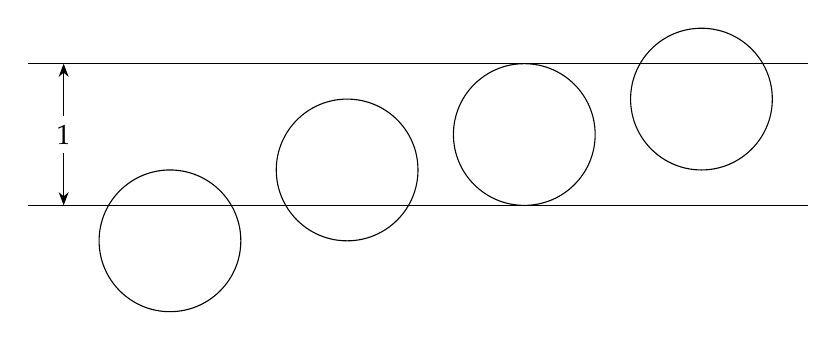
\begin{tikzpicture}[scale=.9]
\draw (0,0) -- (11,0);
\draw (0,2) -- (11,2);
\draw[<->] (.5,0) -- node[fill=white] {$1$} (.5,2);
\foreach \x/\y in {2/-.5, 4.5/.5, 7/1, 9.5/1.5}
  \draw (\x,\y) circle[radius=1];
\end{tikzpicture}
\end{center}
\caption{%
הפתרון של בעיית המחט של Buffon על מעגלים}
\label{f.buffon3}
\end{figure}

תהי 
$E(x)$
התוחלת שמ מספר הקווים המקביליים שקו באורך
$x$
חוצה. עיין עכשיו בקו שמסובבים למעגל
$C$
\textbf{בקוטר}
$1$
והיקף
$\pi$.
אם תזרוק את המעגל על המשטח, הוא יחצה קו 
\textbf{בדיוק}
פעמיים (איור%
~\ref{f.buffon3}),
ולכן:
\begin{equation}\label{eq.buffon-2}
E(C)=2\,.
\end{equation}
בנה מצולע משוכלל
$Q_n$
חסום על ידי 
$c$
(אדום), ובנה מצולע משוכלל 
$R_n$
שחוסם את
$c$
(כחול) (איור%
~\ref{f.buffon4}). 
כל קו ש-%
$Q_n$
חוצה (אדום) חייב לחצות את המעגל וכל קו שחוצה את המעגל (כחול) חייב לחצות את 
$R_n$.
לכן:
\begin{equation}\label{eq.buffon3}
E(Q_n)\leq E(C)\leq E(R_n)\,.
\end{equation}
יהי 
$a_Q, a_R$
סכומי באורכים של צלעות של
$Q_n,R_n$,
בהתאמה. לפי הליניאריות של התוחלת:
{
\addtolength{\arraycolsep}{-3pt}
\begin{eqnarray}\label{eq.buffon1a}
E(Q_n)&=&\sum_{i=1}^n E(a_Q\;\textrm{של צלעות})=a_QE(1)\\
\label{eq.buffon1b}E(R_n)&=&\sum_{i=1}^n E(a_R\;\textrm{של צלעות})=a_RE(1)\,. 
\end{eqnarray}
}
כאשר 
$n\rightarrow\infty$
שני המצולעים הם קירובים למעגל ולכן:
\begin{equation}\label{eq.buffon-pi}
\lim_{n\rightarrow\infty}a_Q = \lim_{n\rightarrow\infty} a_R=\pi\,,
\end{equation}
ההיקף של המעגל. ממשוואות%
~\ref{eq.buffon-2}--\ref{eq.buffon-pi}
מתקבל:
\[
\renewcommand*{\arraystretch}{1.5}
\begin{array}{l}
\lim_{n\rightarrow\infty}E(Q_n)=E(C) =\lim_{n\rightarrow\infty}E(R_n)\\
E(C)=aE(1) =\pi E(1) = 2\\
E(1)=\disfrac{2}{\pi}\\
E(a)=aE(1)=\disfrac{2a}{\pi}\,.
\end{array}
\]
\begin{figure}[bt]
\begin{center}
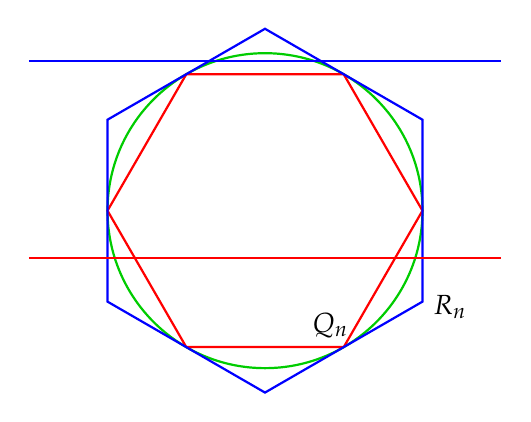
\begin{tikzpicture}
\draw[thick,green!80!black] (0,0) circle[radius=2];
\node[draw,red,thick] (in)
  [minimum size=4cm,regular polygon,regular polygon sides=6]
  at (0,0) {};
\node[draw,blue,rotate=30,thick] (out)
  [minimum size=4.62cm,regular polygon,regular polygon sides=6]
  at (0,0) {};
\node[above left,xshift=5pt] at (in.corner 5) {$Q_n$};
\node[below right,yshift=6pt] at (out.corner 5) {$R_n$};
\draw[thick,red] (-3,-.6) -- +(6,0);
\draw[thick,blue] (-3,1.9) -- +(6,0);
\end{tikzpicture}
\end{center}
\caption{מצולעים כקירובים למעדל}\label{f.buffon4}
\end{figure}

\textbf{סימולציה}

$\pi=2a/E$
ולכן ניתן לחשב קירוב לערכו על ידי הרצת סימולציה או זריקת מחטים על שולחן!
\selectlanguage{english}
\begin{verbatim}
For length = 0.2:
Expectation of crossings = 0.1273
Average crossings        = 0.1308
Empirical value for pi   = 3.0581

For length = 0.5:
Expectation of crossings = 0.3183
Average crossings        = 0.3227
Empirical value for pi   = 3.0989

For length = 1.0:
Expectation of crossings = 0.6366
Average crossings        = 0.6333
Empirical value for pi   = 3.1581
\end{verbatim}
\selectlanguage{hebrew}

%%%%%%%%%%%%%%%%%%%%%%%%%%%%%%%%%%%%%%%%%%%%%%%%%%%%%%%%%%%%%%%%

\begin{prob}{המחט של \L{Buffon} עם רשת אופקי ואנכי}{}{\\(Buffon's needle with horizontal and vertical rulings)}

פתור את בעיית המחט של 
\L{Buffon}
עבור משטח עם רשת אופקי ואנכי כאשר גודל המשבצות הוא 
$1\times 1$.
מחט יכול לחצות קו אנכי (ירוק), קו אופקי (כחול), שניהם (אדום) או אף אחד (כתום) (איור%
~\ref{f.buffon5}).

\begin{figure}[b]
\begin{center}
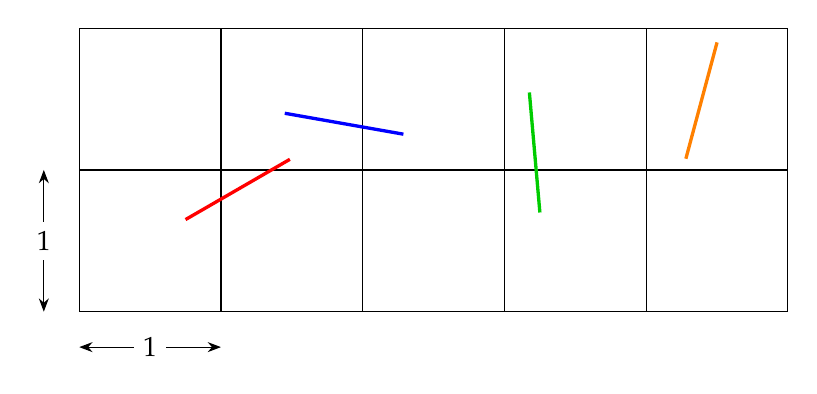
\begin{tikzpicture}[scale=.9]
\draw[step=2cm] (0,0) grid (10,4);
\draw[<->] (-.5,0) -- node[fill=white] {$1$} (-.5,2);
\draw[<->] (0,-.5) -- node[fill=white] {$1$} (2,-.5);
\foreach \x/\y/\a/\c in {
  1.5/1.3/30/red,
  2.9/2.8/-10/blue,
  6.5/1.4/95/green!80!black,
  9/3.8/-105/orange}
    \draw[color=\c,very thick] (\x,\y) -- +(\a:1.7);
\end{tikzpicture}
\end{center}
\caption{בעיית המחט של 
\L{Buffon}
עבור משטח עם רשת אופקי ואנכי}
\label{f.buffon5}
\end{figure}
\end{prob}
\textbf{רמז:}
האם מספר הקווים האופקים והאכנים שהמחט חוצה בלתי-תלויים?

\solution{}

מספר הקווים האופקים והאכנים שהמחט חוצה אכן בלתי-תלויים, ולפי הליניאריות של התוחלת:
\begin{eqn}
E(\textrm{חוצה}\; a\;\textrm{באורך שמחט קווים})&=&
E(\textrm{חוצה}\; a\;\textrm{באורך שמחט אנכים קווים}+\\
&&\quad\; \textrm{\textrm{חוצה}\; a\;\textrm{באורך שמחט אופקים קווים}})\\
&&E(\textrm{חוצה}\; a\;\textrm{באורך שמחט אנכים קווים})+\\
&&E(\textrm{\textrm{חוצה}\; a\;\textrm{באורך שמחט אופקים קווים}})\\
&=&\disfrac{2a}{\pi}+\disfrac{2a}{\pi}=\disfrac{4a}{\pi}\,.
\end{eqn}


%%%%%%%%%%%%%%%%%%%%%%%%%%%%%%%%%%%%%%%%%%%%%%%%%%%%%%%%%%%%%%%%

\begin{prob}{מחטים ארוכים}{D}{(Long needles)}

יהי 
$a>1$
אורכו של המחט בבעייתו של
\L{Buffon}.

\que{1}
מה התוחלת של
\textbf{מספר הקווים}
שמחט חוצה?

\que{2} 
מה ההסתברות שהמחט חוצה
\textbf{לפחות}
קו אחד?

\textbf{רמז:}
עבור איזו זוויות 
$\theta$
ההסתברות של חציית קו היא
$1$?

\end{prob}
\solution{}

\ans{1}
שבור את המחט לחלקים באורים
$\{a_1,a_2,\ldots, a_n\}$, $a_i< 1$,
כך ש-%
$\sum_{i=1}^n a_i=a$.
לפי הליניאריות של התוחלת והפתרון של בעיה~53:
\[
E(a)= \sum_{i=1}^n E(a_i)= \disfrac{2a}{\pi}\,.
\]

\ans{2}
הפתרון מבוסס על
\L{\cite{wiki-buffon}}
ו-%
\L{\cite[Chapter~26]{proofs}}.

לפי משוואה%
~\ref{eq.cross}
ההסתברות שהמחט יחצה קו היא
$a\sin\theta$ 
\textbf{אם}
$a\sin\theta \leq 1$,
כלומר, אם
$0\leq\theta\leq\sin^{-1}(1/a)$.
אבל, אם
$a\sin\theta > 1$
ההסתברות היא
$1$
(איור%
~\ref{f.buffon6}).
נכליל את משוואה%
~\ref{eq.buffon-integral}
עבור
$a>0$
שרירותי. האינטגרל מוחשב בשני חלקים, אחד עבור
$\theta<\sin^{-1}(1/a))$
ואחר עבור
$\theta>\sin^{-1}(1/a))$:
\begin{eqn}
E(a) &=& \disfrac{2}{\pi}
   \left(\int_{0}^{\sin^{-1}(1/a)} 
   a\sin \theta\:d\theta + 
   \int_{\sin^{-1}(1/a)}^{\pi/2} 1\: d\theta\right)\\
&=& \disfrac{2}{\pi}\left(\left.
    a(-\cos \theta)\right|_0^{\sin^{-1}(1/a)} + 
    \left(\disfrac{\pi}{2} - 
    \sin^{-1}(1/a)\right)\right)\\
&=& 1+\disfrac{2}{\pi}
  \left(a
  \left(1-\sqrt{1-\disfrac{1}{a^2}}\right)-
  \sin^{-1}(1/a)\right)\,.
\end{eqn}

\begin{figure}[tb]
\begin{center}
\begin{tikzpicture}[scale=1]
\draw (0,0) -- (10,0);
\draw (0,3.5) -- (10,3.5);
\draw[<->] (.5,0) -- node[fill=white,near end] {$1$} +(0,3.5);
\draw[<->] (5.5,0) -- node[fill=white] {$1/2$} +(0,1.75);
\begin{scope}[xshift=0cm,yshift=1.4cm,scale=1]
\coordinate (end1) at (2,-1);
\coordinate (end2) at ($(end1)+(60:3)$);
\coordinate (center) at ($(end1)+(60:1.5)$);
\node[above right,xshift=2pt,yshift=-2pt]
  at (end1) {$\theta$};
\draw (end1) --  node[left,near end] {$a/2$} (center) -- (end2);
\draw (end2) -- (end2 -| center);
\draw (end1) -- (end1 -| center);
\draw[very thick] (end1 -| center) -- 
  node[right,fill=white,yshift=2pt] {$(a/2)\sin \theta$}
  (center) -- (end2 -| center);
\draw[thick,dotted] (O |- center) -- +(10,0);
\end{scope}
\begin{scope}[xshift=3cm,yshift=.8cm,scale=1.6]
\coordinate (end1) at (2,-1);
\coordinate (end2) at ($(end1)+(60:3)$);
\coordinate (center) at ($(end1)+(60:1.5)$);
\node[above right,xshift=2pt,yshift=-2pt]
  at (end1) {$\theta$};
\draw (end1) --  node[left,near end] {$a/2$} (center) -- (end2);
\draw (end2) -- (end2 -| center);
\draw (end1) -- (end1 -| center);
\draw[very thick] (end1 -| center) -- 
  node[right,fill=white,yshift=6pt] {$(a/2)\sin \theta$}
  (center) -- (end2 -| center);
\end{scope}
\end{tikzpicture}
\end{center}
\caption{מחטים ארוכים}\label{f.buffon6}
\end{figure}

\textbf{סימולציה}
\selectlanguage{english}
\begin{verbatim}
For length = 1.5:
Expectation of crossings = 0.7786
Average crossings        = 0.7780
For length = 2.0:
Expectation of crossings = 0.8372
Average crossings        = 0.8383
For length = 3.0:
Expectation of crossings = 0.8929
Average crossings        = 0.8897
\end{verbatim}
\selectlanguage{hebrew}

%%%%%%%%%%%%%%%%%%%%%%%%%%%%%%%%%%%%%%%%%%%%%%%%%%%%%%%%%%%%%%%%

\begin{prob}{הכד של \L{Molina}}{}{(Molina's urns)}

שני כדים
$U_1,U_2$
מכילים 
$m$
כדורים כל אחד. ב-%
$U_1$
נמצאים 
$w_1$
כדורים לבנים ו-%
$b_1$
כדורים שחורים, וב-%
$U_2$
נמצאים
$w_2$
כדורים לבנים ו-%
$b_2$
כדורים שחורים. מכל כד שלוף
$n$
כדורים
\textbf{עם החזרה}.

\que{1}
עבור ערכים שונים של
$n>1$
מצא
$w_1,b_1,w_2,b_2$
כך ש:
\[
P(\textrm{לבנים}\;U_1\textrm{מ- שנשלפו כדורים כל})=
P(\textrm{שחורים או לבנים}\;U_2\textrm{מ- שנשלפו כדורים כל})\,.
\]
\end{prob}
\solution{}

\ans{1}
עבור 
$n=2$
המשוואה שיש לפתור היא:
\begin{eqn}
\left(\disfrac{w_1}{m}\right)^2&=&\left(\disfrac{w_2}{m}\right)^2+\left(\disfrac{b_2}{m}\right)^2\\
w_1^2&=&w_2^2+b_2^2\,.
\end{eqn}
פתרון אחד הוא
$w_1=10,b_1=4,w_2=6,b_2=8$.

\ans{2}
לפי המשפט האחרון של
\L{Fermat},
שהוכח ב-%
$1995$
על ידי
\L{Andrew Wiles},
אין פתרונות ל-%
$w_1^n=w_2^n+b_2^n$ 
עבור
$n\geq 3$.

%%%%%%%%%%%%%%%%%%%%%%%%%%%%%%%%%%%%%%%%%%%%%%%%%%%%%%%%%%%%%%%%


%% !TeX root = mos-en.tex

%%%%%%%%%%%%%%%%%%%%%%%%%%%%%%%%%%%%%%%%%%%%%%%%%%%%%%%%%%%%%%%%

\begin{prob}{Birthday pairings}
Randomly select $23$ people and ask them what their birthdays are. Assume a uniform distribution of $365$ different birthdays (no one was born on February $29$). Show that the probability that at least two of them have the same birthday is greater than $0.5$.
\end{prob}

\solution{}

Compute the probability that none of the $23$ people have the same birthday and show that it is less than $0.5$. Select the first birthday arbitrarily, then the next birthday from the remaining days, then the next birthday from the remaining days, and so on:
\[
\renewcommand*{\arraystretch}{2.5}
\begin{array}{rcl}
P(\textsf{no birthday pair})&=&
  \overbrace{\disfrac{365}{365}\cdot\frac{364}{365}
  \cdot\frac{363}{365}\cdot \;\cdots \; \cdot \frac{344}{365}
  \cdot\frac{343}{365}}^{23\;\textsf{\small fractions}}\\
&=&\disfrac{365!}{365^{23}\cdot 342!}\approx 0.4927\,.
\end{array}
\]
Most people guess that more than $23$ people are needed to find two with the same birthday!

A modern calculator can compute the probability, but it is worthwhile computing it using Stirling's approximation $\ln n! \approx n\ln n - n$:
\[
\renewcommand*{\arraystretch}{2}
\begin{array}{rcl}
\ln P(\textsf{no birthday pair})&=&
  \ln\left(\disfrac{365!}{342!\cdot 365^{23}}\right)=\ln 365! - \ln 342! -23 \ln 365\\
&\approx& (365\ln 365 -365) - (342\ln 342 -342) - 23\,\ln 365 \\
&\approx&-0.7404\\
P(\textsf{no birthday pair})&\approx&e^{-0.7404}=0.4769\,.
\end{array}
\]
The reader is invited to compute the probability with the following better approximation:
\[
\ln n!  \approx n\ln n - n + \frac{1}{6}\left(8n^3+4n^2+n+\frac{1}{30}\right)+\frac{1}{2}\ln\pi\,.
\]
\textbf{Simulation}
\begin{verbatim}
For 21 people:
Expectation of no pairs = 0.5563
Average no pairs        = 0.5497
For 22 people:
Expectation of no pairs = 0.5243
Average no pairs        = 0.5237
For 23 people:
Expectation of no pairs = 0.4927
Average no pairs        = 0.4933
For 24 people:
Expectation of no pairs = 0.4617
Average no pairs        = 0.4576
For 25 people:
Expectation of no pairs = 0.4313
Average no pairs        = 0.4345
\end{verbatim}

%%%%%%%%%%%%%%%%%%%%%%%%%%%%%%%%%%%%%%%%%%%%%%%%%%%%%%%%%%%%%

\begin{prob}{Finding your birthmate}
Your \emph{birthmate} is a person with the same birthday as yours.

Why is finding a birthmate a different problem than finding a birthday pairing?

\que{1} How many people do you have to ask until the probability of finding your brithmate becomes greater than $0.5$?

\que{2}
Solve the problem by using the approximation in Equation~\ref{eq.reciprocal} (page~\pageref{eq.reciprocal}).
\end{prob}

\solution{}

Many people could have the same birthday which is considered a success for find a birthday pairing, but not for finding a birthmate unless that birthday is the same as yours.

\ans{1}
Find the smallest number of people for which the probability that none of them are birthmates is less than $0.5$. The probability that the first person you ask is not a birthmate is $364/365$, but that is also the probability that the second, third, \ldots, person is not a birthmate. The solution is the smallest $k$ such that:
\[
P(\textsf{birthmate not found})=\left(\frac{364}{365}\right)^k<\frac{1}{2}\,,
\]
which is $k=253$:
\[
\left(\frac{364}{365}\right)^{253} \approx 0.4995\,.
\]
\ans{2}
Equation~\ref{eq.reciprocal} is:
\[
\lim_{n\rightarrow\infty}\left(\frac{n-1}{n}\right)^{n}=\frac{1}{e}\,,
\]
which can be used to approximate the probability:
\begin{eqn}
P(\textsf{birthmate not found})&=&
  \left(\disfrac{365-1}{365}\right)^k=\left[\left(\disfrac{364}{365}\right)^{365}\right]^{k/365}\\
&\approx& e^{-k/365}\\
e^{-253/365}&\approx&0.5000\,.
\end{eqn}
\textbf{Simulation}
\begin{verbatim}
For 251 people:
Probability of no match = 0.5023
Proportion no match     = 0.5120
For 252 people:
Probability of no match = 0.5009
Proportion no match     = 0.5055
For 253 people:
Probability of no match = 0.4995
Proportion no match     = 0.4984
For 254 people:
Probability of no match = 0.4982
Proportion no match     = 0.4987
For 255 people:
Probability of no match = 0.4968
Proportion no match     = 0.5078
\end{verbatim}


%%%%%%%%%%%%%%%%%%%%%%%%%%%%%%%%%%%%%%%%%%%%%%%%%%%%%%%%%%%%%

\begin{prob}{Relating the birthday pairings and the birthmate problems}
Let $P_{\textsf{\footnotesize pair}}(r)$ be the probability that out of $r$ people two are a birthday pair (Problem~$31$) and let $P_{\textsf{\footnotesize mate}}(n)$ be the probability that out of $n$ people at least one is your birthmate (Problem~$32$). Given $r$, for what $n$ does $P_{\textsf{\footnotesize pair}}(r) \approx P_{\textsf{\footnotesize mate}}(n)$?
\end{prob}

\solution{1}

The solution is based on \cite{birthday}.

Using the notation $P_{\textsf{\footnotesize no pair}}(r)$ for the complement of $P_{\textsf{\footnotesize pair}}(r)$, from the solution to Problem~$31$ we have:
\[
\renewcommand*{\arraystretch}{2.2}
\begin{array}{lcl}
P_{\textsf{\footnotesize no pair}}(r)&=&
\disfrac{365}{365}\cdot 
  \frac{365-1}{365}\cdot \frac{365-2}{365} \cdot\;
  \cdots \;\cdot \frac{365-(r-1)}{365}\\
&=&1\left(1-\disfrac{1}{365}\right)
  \left(1-\disfrac{2}{365}\right) \cdot\;
  \cdots \;\cdot \left(1-\disfrac{r-1}{365}\right)\\
&\approx&1-\disfrac{1}{365} - \disfrac{2}{365} -
  \cdots - \disfrac{r-1}{365}\\
&=&1-\disfrac{1+2+3+\cdots + (r-1)}{365}\\
&=&1-\disfrac{r(r-1)/2}{365}\,,
\end{array}
\]
where the approximation in the third equation results from deleting powers of $1/365$ greater than one because they are too small to significantly affect the result.

Using the notation $P_{\textsf{\footnotesize no mate}}(n)$ for the complement and the same approximation, from the solution to Problem~$32$ we have:
\[
\renewcommand*{\arraystretch}{2.2}
\begin{array}{lcl}
P_{\textsf{\footnotesize no mate}}(n)
&=&\overbrace{\left(1-\frac{1}{365}\right)
  \left(1-\frac{1}{365}\right)\cdots
  \left(1-\frac{1}{365}\right)}^{n}\\
&\approx& 1-\overbrace{\frac{1}{365}-\frac{1}{365}\cdots-
  \frac{1}{365}}^{n}\\
&\approx& 1-\disfrac{n}{365}\\
\end{array}
\]
Therefore $P_{\textsf{\footnotesize no pair}}(r)\approx P_{\textsf{\footnotesize no mate}}(n)$ when:
\[
n=\frac{r(r-1)}{2}\,.
\]
For $r=23$, $n=(23\cdot 22)/2=253$.

\solution{2}

Mosteller \cite[p.~322]{birthday} gives the following intuitive solution:
\begin{quote}
In comparing the birthday and birthmate problems, one observes that for $r$ people in the birthday problem, there are $r(r-1)/2$ pairs or \emph{opportunities} for like birthdays; whereas, if $n$ people are questioned in the birthmate problem, there are only $n$ opportunities for me to find one or more birthmates.
\end{quote}
From this he concludes that $n\approx r(r-1)/2$.

This reasoning can be understood as follows: For the birthday problem choose an arbitrary date and ask if two people out of $r$ have \emph{that birthday}. There are:
\[
{r \choose 2}=\frac{r!}{2!(r-2)!} = \frac{r(r-1)}{2}
\]
ways of doing so. For the birthmate problem your own birthday is given. Any of the $n$ people can have the same birthday. By equating the two expressions we have the $n$ such that $P_{\textsf{\footnotesize pair}}(r) \approx P_{\textsf{\footnotesize mate}}(n)$.

\textbf{Simulation}

You can run the simulations using the programs for Problems~31, 32 and check this result.

%%%%%%%%%%%%%%%%%%%%%%%%%%%%%%%%%%%%%%%%%%%%%%%%%%%%%%%%%%%%%

\begin{prob}{Birthday holidays\annotate{D}}
A factory is closed whenever one of its workers has a birthday. There are no other holidays.

\que{1} How many workers should be employed in order to maximize the number of work-days in one year?

\que{2} What is the expectation of the ratio of the maximum work-days to $365^2$, the number of possible work-days if each one of $365$ workers worked every day?

\textbf{Hint:} Prove that there must be a maximum by considering extreme cases. Then develop a formula for the expectation of the number of work-days for a single day.
\end{prob}

\solution{}

\ans{1}
At one extreme if there is only one worker there are $364$ work-days. If there are two workers there are $363+363=726$ workers days (ignoring the very small possibility that both workers have the same birthday). At the other extreme if there are one million workers the number of work-days will almost certainly be zero. Since the number of work-days rises initially and then returns to zero, there must be a maximum in between the extremes.

To simplify the notation we will denote the number of days in a year by $N$ and the number of workers by $n$.

For any given day the probability that it is a work-day is the probability that each worker has a birthday on some other day:
\[
P(\textsf{a given day is a work-day})=\overbrace{\disfrac{N-1}{N} \cdot \;\cdots\;\cdot \disfrac{N-1}{N}}^n = \left(1-\disfrac{1}{N}\right)^n\,.
\]
Denote $\left(1-\disfrac{1}{N}\right)$ by $p$. Then:
\[
E(\textsf{work-days for a given day}) = n \cdot p^n + 0\cdot (1-p^n) = np^n\,.
\]
All the days in the year have this same expectation, so we just multiply by $N$ to get the expectation for a year:
\begin{equation}\label{eq.holidays}
E(\textsf{work-days for a year}) = Nnp^n\,.
\end{equation}

To find the maximum we take the derivative of Equation~\ref{eq.holidays} with respect to $n$ and use $(p^n)'=p^n\ln p$ which can be proved using the chain rule:
\[
(p^n)' = ((e^{\ln p})^n)' =
(e^{n\ln p})' =
e^{n\ln p} (n\ln p)'=
(e^{\ln p})^n \ln p = p^n\ln p\,.
\]
The derivative of Equation~\ref{eq.holidays} is therefore:
\[
(Nnp^n)'= N (p^n + n (p^n)') = N (p^n + np^n\ln p)\,,
\]
which is $0$ when:
\[
n=-\disfrac{1}{\ln p}\,.
\]
For $N=365$ this gives $n=364.5$. Since $n$ is a positive integer the maximum is achieved at $n=364$ or $n=365$ which give the same expectation of the number of work-days:
\begin{eqn}
E(\textsf{work-days for a year}) &=&Nnp^n\\
&=&365\cdot 364 \cdot \left(\disfrac{364}{365}\right)^{364}\\
&=&365\cdot 364  \cdot \disfrac{365}{365}\left(\disfrac{364}{365}\right)^{364}\\
&=&365\cdot 365  \cdot \left(\disfrac{364}{365}\right)^{365}\\
&=&48944\,.
\end{eqn}

\ans{2} 
The expectation of the ratio is:
\[
E(\textsf{max work-days/possible work-days})=\disfrac{365\cdot 365  \cdot \left(\frac{364}{365}\right)^{365}}{365\cdot 365}=\left(\disfrac{364}{365}\right)^{365}\approx 0.3674\,.
\]
By Equation~\ref{eq.reciprocal}:
\[
\lim_{n\rightarrow\infty}E(\textsf{max work-days/possible work-days})=\lim_{N\rightarrow \infty} \left(1-\disfrac{1}{N}\right)= \disfrac{1}{e}\,.
\]

\textbf{Simulation}
\begin{verbatim}
For 100 people
Expectation work-days    = 27742
Average work days        = 27743
Ratio work-days / 365**2 = 0.2082
For 250 people
Expectation work-days    = 45958
Average work days        = 45939
Ratio work-days / 365**2 = 0.3450
For 364 people
Expectation work-days    = 48944
Average work days        = 48936
Ratio work-days / 365**2 = 0.3674
For 365 people
Expectation work-days    = 48944
Average work days        = 48917
Ratio work-days / 365**2 = 0.3674
\end{verbatim}

%%%%%%%%%%%%%%%%%%%%%%%%%%%%%%%%%%%%%%%%%%%%%%%%%%%%%%%%%%%%%

\begin{prob}{The cliff-hanger}
A particle is initially placed on the $x$-axis at position $1$. At any position on the $x$-axis it can move right with probability $2/3$ and left with probability $1/3$ (Figure~\ref{f.ruin1}).

\que{1} What is the probability that the particle will eventually be at position $0$?

\que{2} If the probability of moving right is $p$ and the probability of moving left is $1-p$, what is the probability that the particle will eventually be at position $0$? Analyze the result for various values of $p$.

\textbf{Hint:} Use conditional probabilities after the first move.
\begin{figure}[tb]
\begin{center}
\begin{tikzpicture}[scale=1.5]
\draw (0,0) -- (6,0);
\draw[dashed] (6,0) -- (8,0) node[right] {$\infty$};
\foreach \x in {0,1,2,3,4,5,6} {
  \draw (\x,0) -- +(0,4pt);
  \node at (\x,-10pt) { $\x$ };
}
\draw[fill] (1,5mm) circle[radius=.5pt];
\draw[->] (1,5mm) -- node[above] {$1/3$} (0,5mm);
\draw[->,very thick] (1,5mm) -- node[above] {$2/3$} (2,5mm);

\foreach \x/\y in {2/10mm,3/15mm,4/20mm} {
  \draw[fill] (\x,\y) circle[radius=.5pt];
  \draw[->] (\x,\y) -- node[above] {$1/3$} (\x-1,\y);
  \draw[->] (\x,\y) -- node[above] {$2/3$} (\x+1,\y);
}
\end{tikzpicture}
\end{center}
\caption{Can the particle return to $0$ (axis is infinite to the right)?}\label{f.ruin1}
\end{figure}
\end{prob}

\solution{}

It is no more difficult to compute the probabilty for arbitrary $p$ as it is for $p=2/3$, so we give solutions for both questions together.

\ans{1,2}
Let us try to compute the probability directly. Denote a move left by $L$ and a move right by $R$. The particle can reach $0$ directly by moving $L$ with probability $\frac{1}{3}$, or by moving $RLL$ with probability $\frac{2}{3}\cdot\frac{1}{3}\cdot\frac{1}{3}$, or by moving $RRLLL$ with probability $\left(\frac{2}{3}\right)^2\left(\frac{1}{3}\right)^3$, \ldots\ . This computations seems to be a straightforward geometric progression, but it ignores possibilities such as $RLRLL$.

Compute the probability that the particle reaches $0$ from $1$ conditioned on the first step:
\begin{eqn}
P(\textsf{reaches}\;0\;\textsf{from}\;1) &=& P(\textsf{reaches}\;0\;\textsf{from}\;1|\textsf{first move left}) +\\
&&P(\textsf{reaches}\;0\;\textsf{from}\;1|\textsf{first move right})\\
&=& (1-p)\cdot 1 + pP(\textsf{reaches}\;1\;\textsf{from}\;2)P(\textsf{reaches}\;0\;\textsf{from}\;1)\,.
\end{eqn}
But the probability of reaching $1$ from $2$ is exactly the same as the probability of reaching $0$ from $1$. Denoting $P(\textsf{reaches}\;0\;\textsf{from}\;1)$ by $P$ we have:
\begin{eqn}
P &=& (1-p) + pP^2\\
pP^2 - P + (1-p) &=&0\\
P&=& \frac{1\pm\sqrt{1-4p(1-p)}}{2p}\\
P&=&1,\; (1-p)/p\,.
\end{eqn}
If $p\leq 1/2$ then $(1-p)/p\geq 1$, so $P=1$ is the only solution and it is certain that the particle will reach $0$.

If $p=1$ then $P=0$ since if the particle always moves to the right it cannot return to $0$.

Suppose $P=1$ for $1/2<p < 1$, that is, $P$ \emph{does not depend on} $p$. But $P$ cannot suddenly ``jump'' from $1$ to $0$ as $p$ approaches $1$: in Figure~\ref{f.ruin2} the dashed red line and the red dot at $(1,0)$. Therefore, for $p> 1/2$ the only solution is $P=(1-p)/p< 1$.\footnote{Mosteller writes that this follows by continuity but does not give a proof.}

\begin{figure}[tb]
\begin{center}
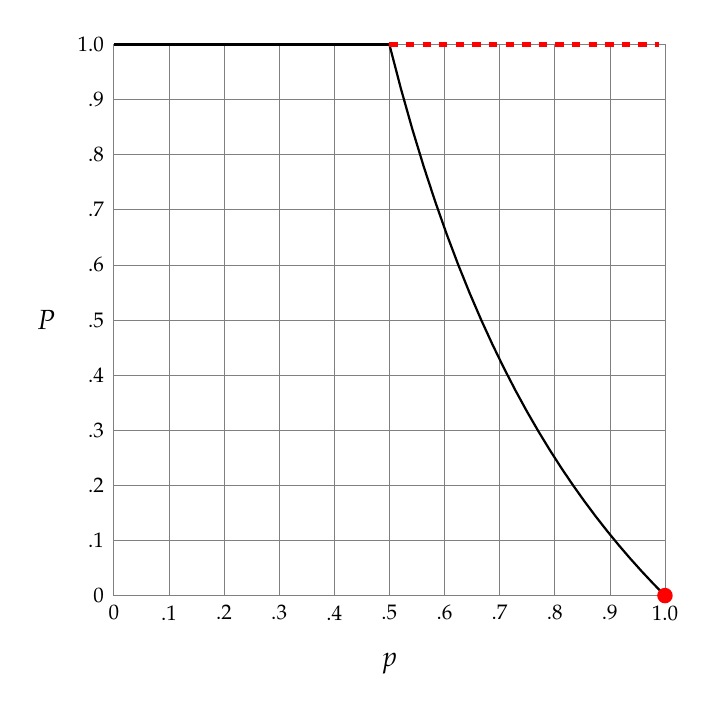
\begin{tikzpicture}[scale=7]
\draw[help lines,step=.1] (0,0) grid (1,1);
\foreach \x in {0,.1,.2,.3,.4,.5,.6,.7,.8,.9,1.0}
  \node[below] at (\x,0) {$\scriptstyle \x$};
\foreach \y in {0,.1,.2,.3,.4,.5,.6,.7,.8,.9,1.0}
  \node[left] at (0,\y) {$\scriptstyle \y$};
\draw[domain=0:.5,thick] plot (\x,1);
\draw[domain=.5:1,thick] plot (\x,{(1-\x)/\x});
\node at (.5,-3.5pt) {$p$};
\node at (-3.5pt,.5) {$P$};
\draw[ultra thick,red,dashed] (.5,1) -- +(.49,0);
\fill[red] (1,0) circle[radius=.4pt];
\end{tikzpicture}
\end{center}
\caption{Graph of $P=\min(p/(1-p),1)$ for $p\in [0,1]$}\label{f.ruin2}
\end{figure}
For $p=2/3, P=1/2$ and for $p=1/2, P=1$. This is a surprising result because one would not expect that the particle would always return to $0$ if the direction of the moves were determined by flipping a fair coin! You have to have a very unfair coin (probability of heads is $2/3$) to even the chances or returning to $0$ or not.

\textbf{Simulation}
\begin{verbatim}
For probability = 0.2500:
Probability of reaching 0 = 1.0000
Proportion reaching 0     = 1.0000
For probability = 0.5000:
Probability of reaching 0 = 1.0000
Proportion reaching 0     = 0.9612
For probability = 0.6667:
Probability of reaching 0 = 0.5000
Proportion reaching 0     = 0.5043
For probability = 0.7500:
Probability of reaching 0 = 0.3333
Proportion reaching 0     = 0.3316
For probability = 0.8000:
Probability of reaching 0 = 0.2500
Proportion reaching 0     = 0.2502
\end{verbatim}

%%%%%%%%%%%%%%%%%%%%%%%%%%%%%%%%%%%%%%%%%%%%%%%%%%%%%%%%%%%%%

\begin{prob}{Gambler's ruin\annotate{D}}
A particle is initially placed on the $x$-axis at position $m\geq 1$. At any position on the $x$-axis it can move right with probability $p>1/2$ and left with probability $1-p$.

\que{1} What is the probability that the particle will eventually be at position $0$?

\que{2} Let $n>m$. If the particle reaches position $0$ or position $n$ its stops moving (Figure~\ref{f.ruin3}). What is the probability that the particle will eventually be at position $0$? What is the probability that the particle will eventually be at position $n$?
\begin{figure}[tb]
\begin{center}
\begin{tikzpicture}[scale=1.5]
\draw (0,0) -- (6,0);
\foreach \x in {0,1,2,3,4,5,6} {
  \draw (\x,0) -- +(0,4pt);
  \node at (\x,-10pt) { $\x$ };
}
\node at (2,-20pt) {$m$};
\node at (6,-20pt) {$n$};
\draw[fill] (2,5mm) circle[radius=.5pt];
\draw[->] (2,5mm) -- node[above] {$1/3$} (1,5mm);
\draw[->] (2,5mm) -- node[above] {$2/3$} (3,5mm);
\end{tikzpicture}
\end{center}
\caption{Can the particle return to $0$ (axis is finite)?}\label{f.ruin3}
\end{figure}

\textbf{Note:} Problem~35 is represents a gambler with a finite amount of money playing against a casino with unlimited money. The problem asks for the probabiliy that the gambler loses all his money. This problem represents one gambler who starts with $m$ playing against a second gambler who starts with $n-m$. The problem asks for the probabilities that \emph{one} of the gamblers loses all her money to the other one.
\end{prob}

\solution{}

The solution is based on \cite[Chapter~2, Example~4m]{ross}.

\ans{1} The solution to Problem~35 showed that for $p>1/2$ (here it is given), if a particle is at position $1$ the probability of its reaching position $0$ is $r=(1-p)/p$. Notation: let $P(i,j)$ be the probability of reaching $i$ from $j$. Since the probability of a particle reaching one position from another does not depend on the absolute position:
\begin{equation}
P(0,m)=P(m-1,m)P(m-2,m-1)\cdots P(1,2)P(0,1)=r^m\,.
\end{equation}

\ans{2} Let $P_i=P(n,i)$ and compute it using conditional probability:
\begin{eqn}
P_i &=& pP_{i+1} + (1-p)P_{i-1}\\
pP_{i+1}&=&1\cdot P_i - (1-p)P_{i-1}\\
pP_{i+1}&=&(p+(1-p))P_i - (1-p)P_{i-1}\\
p(P_{i+1}-P_i)&=&(1-p)(P_i-P_{i-1})\\
P_{i+1}-P_i&=&r(P_i-P_{i-1})\,.
\end{eqn}
$P_0=0$ since if the particle is at $0$ it does not move. Therefore:
\begin{eqn}
P_2 - P_1 &=& r(P_1 - P_0) = rP_1\\
P_3 - P_2 &=& r(P_2 - P_1) = r^2P_1\\
\cdots &=&\cdots\\
P_i - P_{i-1} &=& r(P_{i-1} - P_{i-2}) = r^{i-1}P_1\,.
\end{eqn}
Most of the terms on the lefthand sides cancel when we add the equations:
\begin{eqn}
P_i - P_1 &=& P_1\sum_{j=2}^{i}r^{j-1}\\
&=& P_1 + P_1\sum_{j=2}^{i}r^{j-1} - P_1 \\
P_i&=& P_1\sum_{j=0}^{i-1}r^j =P_1\left(\frac{1-r^i}{1-r}\right)\,.
\end{eqn}
If the particle is at $n$ then it is already at $n$ so $P_n=1$:
\begin{eqn}
1 &=& P_1\left(\frac{1-r^n}{1-r}\right)\\
P_1 &=& \left(\frac{1-r}{1-r^n}\right)\,,
\end{eqn}
and therefore (using a symmetrical argument exchanging $p$ and $1-p$):
\begin{eqnlabels}
\label{eq.ruin1}P(n,i) &=& \left(\frac{1-r^{i}}{1-r^n}\right)\\
\label{eq.ruin2}P(0,i) &=& \left(\frac{1-(1/r)^{n-i}}{1-(1/r)^{n}}\right)\,.
\end{eqnlabels}
We leave it to the reader to show that the sum of Eqs.~\ref{eq.ruin1},~\ref{eq.ruin2} is $1$ meaning that one of the players will certainly win and one will lose. For $m=1, n=3, p=2/3$:
\begin{eqn}
P(0,1) &=& \left(\frac{1-\left(\frac{1}{2}\right)^{1}}{1-\left(\frac{1}{2}\right)^{3}}\right)=\frac{4}{7}\\
P(3,1) &=& \left(\frac{1-2^{2}}{1-2^{3}}\right)=\frac{3}{7}\,.
\end{eqn}

\textbf{Simulation}
\begin{verbatim}
For probability = 0.6667:
Probability of reaching (0,10) from 1 = (0.4995,0.5005)
Proportion reaching     (0,10) from 1 = (0.5056,0.4944)
Probability of reaching (0,10) from 4 = (0.0616,0.9384)
Proportion reaching     (0,10) from 4 = (0.0643,0.9357)
Probability of reaching (0,10) from 6 = (0.0147,0.9853)
Proportion reaching     (0,10) from 6 = (0.0123,0.9877)
\end{verbatim}

\begin{verbatim}
For probability = 0.7500:
Probability of reaching (0,10) from 1 = (0.3333,0.6667)
Proportion reaching     (0,10) from 1 = (0.3395,0.6605)
Probability of reaching (0,10) from 4 = (0.0123,0.9877)
Proportion reaching     (0,10) from 4 = (0.0115,0.9885)
Probability of reaching (0,10) from 6 = (0.0014,0.9986)
Proportion reaching     (0,10) from 6 = (0.0015,0.9985)
\end{verbatim}
The greater the amount of money that the left player has and the greater his probability of winning each bet, the higher his probability of winning.

\textbf{Plot of steps}

This plot was generated by the Python library \texttt{matplotlib}; the source code appears in the file \texttt{36-gamblers-ruin-plot.py}.
\begin{center}
% This file was created with tikzplotlib v0.10.1.
\begin{tikzpicture}

\definecolor{darkgray176}{RGB}{176,176,176}
\definecolor{steelblue31119180}{RGB}{31,119,180}

\begin{axis}[
tick align=outside,
tick pos=left,
title={m = 20, n = 50, p = 0.67 מהמר של הרגל פשיטת},
x grid style={darkgray176},
xlabel={צעדים},
xmin=-7.5, xmax=157.5,
xtick style={color=black},
y grid style={darkgray176},
ylabel={מקום},
ymin=0, ymax=52,
ytick style={color=black}
]
\addplot [thick, steelblue31119180]
table {%
0 21
1 22
2 23
3 24
4 23
5 22
6 23
7 22
8 23
9 24
10 25
11 26
12 27
13 26
14 27
15 26
16 25
17 26
18 27
19 28
20 27
21 28
22 27
23 28
24 27
25 28
26 27
27 26
28 27
29 28
30 29
31 30
32 31
33 32
34 33
35 34
36 35
37 34
38 35
39 34
40 35
41 34
42 33
43 34
44 33
45 34
46 33
47 32
48 31
49 30
50 31
51 30
52 31
53 30
54 31
55 32
56 33
57 34
58 35
59 36
60 37
61 36
62 37
63 38
64 37
65 36
66 37
67 38
68 39
69 40
70 39
71 40
72 41
73 40
74 41
75 42
76 43
77 42
78 41
79 42
80 43
81 44
82 43
83 44
84 45
85 46
86 47
87 46
88 47
89 48
90 49
91 50
92 50
93 50
94 50
95 50
96 50
97 50
98 50
99 50
100 50
101 50
102 50
103 50
104 50
105 50
106 50
107 50
108 50
109 50
110 50
111 50
112 50
113 50
114 50
115 50
116 50
117 50
118 50
119 50
120 50
121 50
122 50
123 50
124 50
125 50
126 50
127 50
128 50
129 50
130 50
131 50
132 50
133 50
134 50
135 50
136 50
137 50
138 50
139 50
140 50
141 50
142 50
143 50
144 50
145 50
146 50
147 50
148 50
149 50
150 50
};
\end{axis}

\end{tikzpicture}

\end{center}

%%%%%%%%%%%%%%%%%%%%%%%%%%%%%%%%%%%%%%%%%%%%%%%%%%%%%%%%%%%%%

\begin{prob}{Bold play vs. cautious play}
In roulette you can bet that the ball will fall into a pocket with an even number. The probability is $18/38$ since there are $18$ even numbers, $18$ odd numbers and $2$ green numbers where the casino wins.

Which of the following strategies is better?
\begin{enumerate}
\item Bold play: betting $20$ in one round.
\item Cautious play: bettin $1$ per round until you win or lose $20$.
\end{enumerate}
\textbf{Hint:} Use the results of Problem~36.
\end{prob}

\solution{}

The probability of winning with bold play is $18/38\approx 0.4737$.

The probability of winning with cautious play is (Equation~\ref{eq.ruin1}):
\begin{eqn}
r&=&\frac{20}{38}\Big/ \frac{18}{38}=\frac{20}{18}\\
P(40,20) &=&
\frac{1-(20/18)^{20}}{1-(20/18)^{40}}\approx 0.1084\,.
\end{eqn}
Clearly, bold play is preferable to cautious play.

Mosteller writes that the intuitive explanation for this result is that betting in more rounds exposes the player to the probability of $2/38$ that the casino wins.

\textbf{Simulation}
\begin{verbatim}
Probability of bold wins     = 0.4737
Proportion bold wins         = 0.4677
Probability of cautious wins = 0.1084
Proportion cautious wins     = 0.1094
\end{verbatim}

%%%%%%%%%%%%%%%%%%%%%%%%%%%%%%%%%%%%%%%%%%%%%%%%%%%%%%%%%%%%%

\refstepcounter{problem}

%%%%%%%%%%%%%%%%%%%%%%%%%%%%%%%%%%%%%%%%%%%%%%%%%%%%%%%%%%%%%

\begin{prob}{The clumsy chemist}

You have a large number of glass rods of length $1$ with one end colored red and the other colored blue. When you drop them on the floor they each break into three pieces with a uniform distribution of the length of the pieces (Figure~\ref{f.rod1}). What is the expectation of the length of the piece whose end is colored blue?

\textbf{Hint:}
Instead of straight rods suppose that you are given (unmarked) glass rings that also break into three pieces (Figure~\ref{f.rod2}).
\begin{figure}[tb]
\begin{center}
\begin{subfigure}{.4\textwidth}
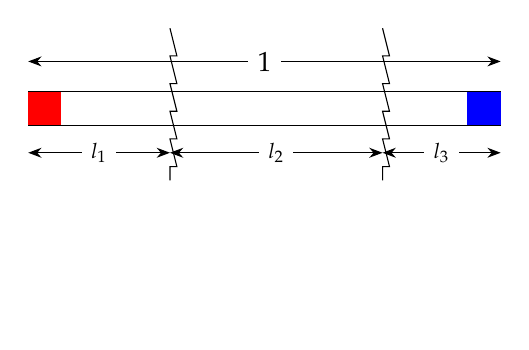
\begin{tikzpicture}
\draw (0,0) -- ++(6,0) -- ++(0,12pt) -- ++(-6,0) -- cycle;
\fill[red] (0,0) rectangle +(12pt,12pt);
\fill[blue] (6,0) rectangle +(-12pt,12pt);
\draw[<->] (0,23pt) --
  node[fill=white] {$1$} ++(6,0);
\draw[decorate,decoration=saw] (1.8,35pt) -- +(0,-55pt);
\draw[decorate,decoration=saw] (4.5,35pt) -- +(0,-55pt);
\draw[<->] (0,-10pt) --
  node[fill=white] {$\scriptstyle l_1$} (1.8,-10pt);
\draw[<->] (1.8,-10pt) --
  node[fill=white] {$\scriptstyle l_2$} (4.5,-10pt);
\draw[<->] (4.5,-10pt) --
  node[fill=white] {$\scriptstyle l_3$} (6,-10pt);
\path (0,-1) rectangle +(2,-1.5);
\end{tikzpicture}
\caption{Breaking a rod into three pieces}\label{f.rod1}
\end{subfigure}
\hspace{3em}
\begin{subfigure}[b]{.4\textwidth}
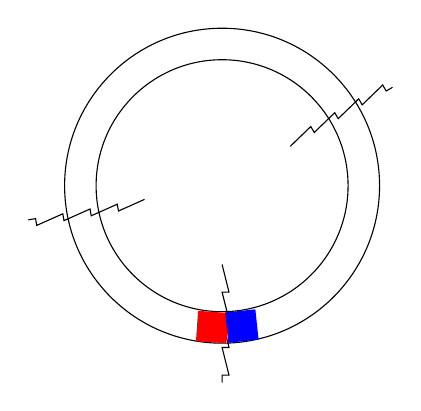
\begin{tikzpicture}
\draw (0,0) circle[radius=2];
\draw (0,0) circle[radius=1.6];
\draw[decorate,decoration=saw] (30:1) -- +(30:1.5);
\draw[decorate,decoration=saw] (190:1) -- +(190:1.5);
\draw[decorate,decoration=saw] (-90:1) -- +(-90:1.5);
\node[rotate=-4,fill=red,minimum width=11pt,minimum height=11pt]
  at (-94:1.8) {};
\node[rotate=6,fill=blue,minimum width=11pt,minimum height=11pt]
  at (-82:1.8) {};
\end{tikzpicture}
\caption{Breaking a ring into three pieces}\label{f.rod2}
\end{subfigure}
\end{center}
\end{figure}
\end{prob}

\solution{1}

The rods are not symmetric because the end pieces are different from the center piece. However, the ring is symmetric so the distributions of all three pieces must be uniform with expectation $1/3$. By choosing and coloring one of breaks as shown in Figure~\ref{f.rod2}, the problem is now the same as that of the rods so the distributions remain the same. Therefore the expectation of the lengths of the pieces is also $1/3$.

\solution{2}

Here is an elegant solution from \cite{stack-rods}.

Assume that the rod represents the line segment $(0,1)$. The rod is broken in two places which are represented as two uniform independent random variables $X,Y\in (0,1)$. Let us compute the probability $P(|X-Y|>a)$.

Table~\ref{t.rods} shows points $(x,y)$, where $x,y \in \{0.0, 0.1, 0.2, \ldots, 0.9\}$ and the decimal point is omitted. The values that appear in the table are $|X-Y|$. For $a=0.6$ the entries in the upper left corner $(0,6)$--$(6,9)$ and above, and the entries in the lower right corner $(6,0)$--$(9,6)$ and below, are those outcomes that define $P(|X-Y|>a)$:
\[
P(|X-Y|>a)=2\cdot \frac{1}{2}(1-a)(1-a)=(1-a)^2\,.
\]
For $a=0.6$, $P(|X-Y|>0.6)=(0.4)^2=0.16$.

\begin{table}[bt]
\[
\begin{array}{c}
\quad\\\\\\
a\\\\
\quad\\
y\\
\quad\\\quad\\\quad\\\quad
\end{array}
\begin{array}{|c|cccccccccc|}
\multicolumn{11}{l}{\qquad \qquad \qquad a}\\
\hline
9& 9 & 8 & 7 & 6 & 5 & 4 & 3 & 2 & 1 & 0  \\
8& 8 & 7 & 6 & 5 & 4 & 3 & 2 & 1 & 0 & 1  \\
7& 7 & 6 & 5 & 4 & 3 & 2 & 1 & 0 & 1 & 2  \\
6& 6 & 5 & 4 & 3 & 2 & 1 & 0 & 1 & 2 & 3  \\
5& 5 & 4 & 3 & 2 & 1 & 0 & 1 & 2 & 3 & 4  \\
4& 4 & 3 & 2 & 1 & 0 & 1 & 2 & 3 & 4 & 5  \\
3& 3 & 2 & 1 & 0 & 1 & 2 & 3 & 4 & 5 & 6  \\
2& 2 & 1 & 0 & 1 & 2 & 3 & 4 & 5 & 6 & 7  \\
1& 1 & 0 & 1 & 2 & 3 & 4 & 5 & 6 & 7 & 8  \\
0& 0 & 1 & 2 & 3 & 4 & 5 & 6 & 7 & 8 & 9  \\
\hline
&0 & 1 & 2 & 3 & 4 & 5 & 6 & 7 & 8 & 9  \\
\hline
\multicolumn{11}{c}{\quad \quad x\quad\quad\quad a}
\end{array}
\begin{array}{c}
\\\\\\
a\\\\
\end{array}
\]
\caption{Distribution of breaks on $(0,1)\times (0,1)$}\label{t.rods}
\end{table}

Taking the complement gives:
\[
P(|X-Y|<a)=1-(1-a)^2\,.
\]
This is the cumulative probability distribution (CPD) for the interval $(0,1)$. The probability density function (PDF) can be obtained by differentiating the CDP:
\[
P(|X-Y|=a)= \frac{d}{da}P(|X-Y|<a) =
  \frac{d}{da}(1-(1-a)^2)=2(1-a)\,.
\]
The expectation is the integral of the PDF multiplied by the value:
\[
E(|X-Y|)= \int_{0}^{1} a\cdot2(1-a)\, da=
  2\left.\left(\frac{a^2}{2}-\frac{a^3}{3}\right)\right|_0^1=\frac{1}{3}\,.
\]

\textbf{Simulation}
\begin{verbatim}
Expectation of length of right piece = 0.3333
Average length of right piece        = 0.3359
\end{verbatim}

%%%%%%%%%%%%%%%%%%%%%%%%%%%%%%%%%%%%%%%%%%%%%%%%%%%%%%%%%%%%%

\begin{prob}{The first ace}
Deal cards from a well-shuffled deck of cards until an ace appears. What is the expectation of the number of cards that must be dealt?

\textbf{Hint:} Consider the deck of cards without the aces to be laid out in a line.
\end{prob}

\solution{}

The cards form a ``rod'' of length $48$ which is ``broken'' by the $4$ aces into $5$ ``pieces.'' The solution of Problem~39 applies and the expectation of the length of a piece is $48/5=9.6$.

\textbf{Simulation}
\begin{verbatim}
Expectation of first ace = 9.6000
Average first ace        = 9.5805
\end{verbatim}

%%%%%%%%%%%%%%%%%%%%%%%%%%%%%%%%%%%%%%%%%%%%%%%%%%%%%%%%%%%%%


%% !TeX root = mos-he.tex

%%%%%%%%%%%%%%%%%%%%%%%%%%%%%%%%%%%%%%%%%%%%%%%%%%%%%%%%%%%%%%%%

\refstepcounter{problem}  % 41. The locomotive problem

%%%%%%%%%%%%%%%%%%%%%%%%%%%%%%%%%%%%%%%%%%%%%%%%%%%%%%%%%%%%%%%%

\begin{prob}{הקצה הקצר של המקל}{S}{(The little end of the stick)}

אתה שובר מספר גדול של מקלות זכוכית באורך $1$ לשני חלקים. למקום השבירה התפלגות אחידה לאורך המקל.


\que{1} 
מה התוחלת של אורכו של החלק 
\textbf{הקטן}
יותר?

\que{2} 
מה התוחלת של היחס בין אורכו של החלק הקטן לאורכו של החלק הגדול?
\end{prob}

\solution{}

\ans{1}
ההסתברות שנקודת השבירה היא בצד השמאלי של המקל היא
$1/2$
שהיא גם ההסתברות שהנקודה בצד ימין. החלק הקטן יותר נמצא באותו צד שבו נמצאת נקודת השבירה. התוחלת של נדוקת השבירה היא באמצע בין קצה המקל לבין אמצע המקל:
\[
E(\textrm{יותר הקטן אורך}) = \frac{1}{2}\cdot\frac{1}{2}=\frac{1}{4}\,.
\]

\ans{2}
ללא הגבלת הכלליות הנח שנקודת השבירה נמצאת בצד הימני של המקל (איור%
~\ref{f.stick}).
היחס בין החלק הקטן והחלק הגדול הוא
$(1-x)/x$
ואורכו של החלק הגדול מתפלג אחיד בתוך
$(1/2,1)$. 
לכן:
\begin{eqn}
E(\textrm{יותר קטן / יותר גדול יחס})&=&\left(\frac{1}{1-(1/2)}\right)\int_{1/2}^1 \frac{1-x}{x} \,dx\\
&=& 2\int_{1/2}^1 \left(\frac{1}{x} -1\right) \,dx \\
&=& 2\left.(\ln |x| - x)\right|_{1/2}^1 = 2\ln 2 -1\approx 0.3863\,.
\end{eqn}
\begin{figure}[tb]
\begin{center}
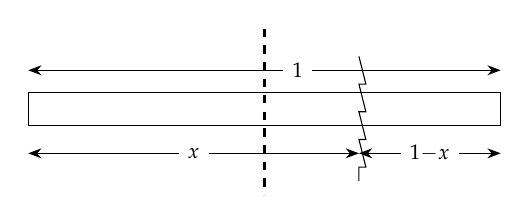
\begin{tikzpicture}
\draw (0,0) -- ++(6,0) -- ++(0,12pt) -- ++(-6,0) -- cycle;
\draw[<->] (0,20pt) --
  node[fill=white,xshift=12pt] {$\scriptstyle 1$} ++(6,0);
\draw[decorate,decoration=saw] (4.2,25pt) -- +(0,-45pt);
\draw[thick,dashed] (3,35pt) -- +(0,-60pt);
\draw[<->] (0,-10pt) --
  node[fill=white] {$\scriptstyle x$} (4.2,-10pt);
\draw[<->] (4.2,-10pt) --
  node[fill=white] {$\scriptstyle 1-x$} (6,-10pt);
\end{tikzpicture}
\end{center}
\caption{שבירת מקל לשני חלקים}\label{f.stick}
\end{figure}

\textbf{סימולציה}
\selectlanguage{english}
\begin{verbatim}
Expectation of length of smaller = 0.2500
Average length of smaller        = 0.2490
Expectation of smaller/larger    = 0.3863
Average smaller/larger           = 0.3845
\end{verbatim}
\selectlanguage{hebrew}

%%%%%%%%%%%%%%%%%%%%%%%%%%%%%%%%%%%%%%%%%%%%%%%%%%%%%%%%%%%%%%%%


\begin{prob}{המקל השבור}{D,S}{(The broken bar)}

אתה שובר מספר רב של מקלות זכוכית באורך 
$1$
בשתי נדוקות שבירה (איור%
~\ref{f.break1}).

\que{1} 
מה התוחלת של אורכו של החלק הקצר ביותר?

\que{2} 
מה התוחלת של אורכו של החלק הארוך ביותר?

\textbf{רמז:}
$x,y$
הם משתנים אקראים בלתי-תלויים בהתפלגות אחידה בתוך 
$(0,1)$.
ניתן להציג כל זוג
$(x,y)$
כנקודה בריבוע
$(0,1)\times (0,1)$ 
(איור%
~\ref{f.break2}).
מה ההסתברות ש-%
$(x,y) < (.5,.25)$? 

\textbf{Hint:}
עבור 
\que{1}
הנח שהחלק השמאלי הוא הקצר ביותר ועבור 
\que{2}
הנח שהחלק השמאלי הוא בארוך ביותר.
\begin{figure}[tb]
\centering
\selectlanguage{hebrew}
\subcaptionbox{%
חלוקת מקל לשני חלקים%
\label{f.break1}}
[.45\textwidth]
{
\centering
\begin{tikzpicture}[scale=.75]
\draw (0,0) node[below left] {$0$} --
  ++(6,0) node[below right] {$1$} --
  ++(0,12pt) -- ++(-6,0) -- cycle;
\draw[<->] (0,20pt) --
  node[fill=white] {$\scriptstyle 1$} ++(6,0);
\draw[decorate,decoration=saw] (1.8,25pt) -- +(0,-45pt);
\draw[decorate,decoration=saw] (4.7,25pt) -- +(0,-45pt);
\node[below left] at (1.8,0) {$x$};
\node[below left] at (4.7,0) {$y$};
\path (0,-3.5) rectangle +(0,3.5);
\end{tikzpicture}
}
\hspace{3em}
\subcaptionbox{%
יצוג האורכים במעגל היחידה%
\label{f.break2}}
[.45\textwidth]
{
\centering
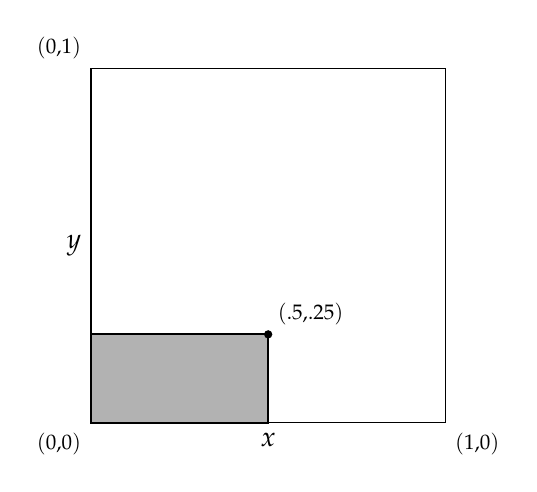
\begin{tikzpicture}[scale=.75]
\draw (-3,-3) rectangle +(6,6);
\draw[thick,fill=white!70!black] (-3,-3) -- ++(0,1.5) -- 
  ++(3,0) -- ++(0,-1.5) -- cycle;
\path (-3,-3) node[below left] {$\scriptstyle (0,0)$} --
  node[below] {$x$} (3,-3)
  node[below right] {$\scriptstyle (1,0)$};
\path (-3,-3) -- node[left] {$y$} (-3,3)
  node[above left] {$\scriptstyle (0,1)$};
\fill (0,-1.5) circle [radius=2pt]
  node[above right] {$\scriptstyle (.5,.25)$};
\end{tikzpicture}
}
\end{figure}
\end{prob}

\solution{}

\ans{1}
ללא הגבלת הכלליות הנח שהחלק השמאלי שאורכו 
$x$
הוא החלק הקצר ביותר. מכאן ש-%
$x<y-x$
ו-%
$x < 1-y$
שניתן לפשט ולקבל
$2x<y$
ו-%
$x+y<1$.

איור%
~\ref{f.shaded1}
מראה את הקווים
$y=2x$
(אדום) ו-%
$y=1-x$
(כחול). כדי לאמת את אי-השוויונות, 
$(x,y)$
חייבת להיות באיזור באפור לשמאל לשני הקווים. ניתן לחשב את נקודת החיתוך
$(1/2,2/3)$
על ידי פתרון שתי המשוואות.

הערכים של 
$(x,y)$
נמצאים בריבוע
$(0,1)\times(0,1)$,
ולכן יש לחשב את התוחלת מעל לתת-קבוצה האפורה של הריבוע על ידי חילוק האינטגרל בשטח של האיזור האפור
$\frac{1}{2} (\frac{1}{3}\cdot 1)=\frac{1}{6}$:
\begin{eqn}
E(x)&=& \frac{1}{1/6}\int_{0}^{1/3} x [(1-x)-2x]\,dx\\
&=&\int_{0}^{1/3} (6x -18x^2)\,dx\\
&=&\left. (3x^2-6x^3)\right|_0^{1/3}=\disfrac{2}{18}\approx 0.1111\,.
\end{eqn}

\begin{figure}[tb]
\centering
\selectlanguage{hebrew}
\subcaptionbox{%
איזור אפור עבור המקל הקצר ביותר%
\label{f.shaded1}}
[.45\textwidth]
{
\centering
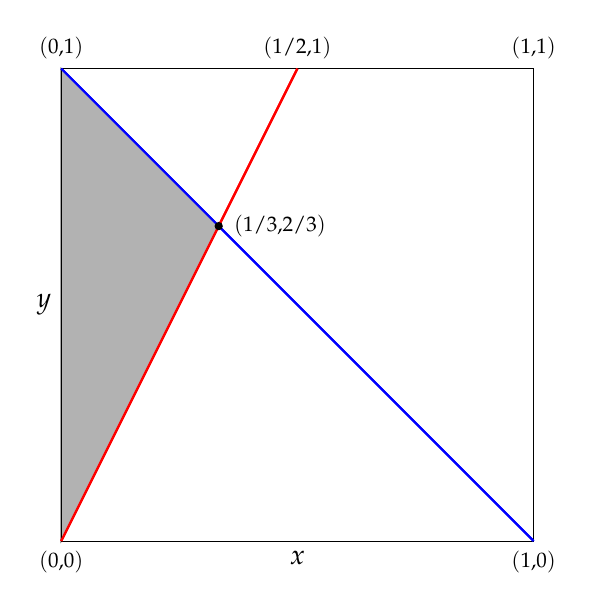
\begin{tikzpicture}[scale=1]
\draw (-3,-3) rectangle +(6,6);
\path (-3,-3) node[below] {$\scriptstyle (0,0)$} --
  node[below] {$x$} (3,-3)
  node[below] {$\scriptstyle (1,0)$};
\path (-3,-3) -- node[left] {$y$} (-3,3)
  node[above] {$\scriptstyle (0,1)$};
\draw[red,thick]  (-3,-3) -- (0,3);
\draw[blue,thick] (-3,3)  -- (3,-3);
\coordinate (P) at (-1,1);
\draw[fill=white!70!black] (-3,-3) -- (P) -- 
  (-3,3) -- cycle;
\draw[red,thick]  (-3,-3) -- (0,3);
\draw[blue,thick] (-3,3)  -- (3,-3);
\fill (P) circle[radius=1.5pt]
  node[right,xshift=2pt] {$\scriptstyle (1/3,2/3)$};
%\draw[thick,dotted] (-3,-3) -- (3,3);
\node[above] at(0,3) {$\scriptstyle (1/2,1)$};
\node[above] at(3,3) {$\scriptstyle (1,1)$};
\end{tikzpicture}
}
\hspace{1em}
\subcaptionbox{%
איזור אפור עבור המקל הארוך ביותר%
\label{f.shaded2}}
[.45\textwidth]
{
\centering
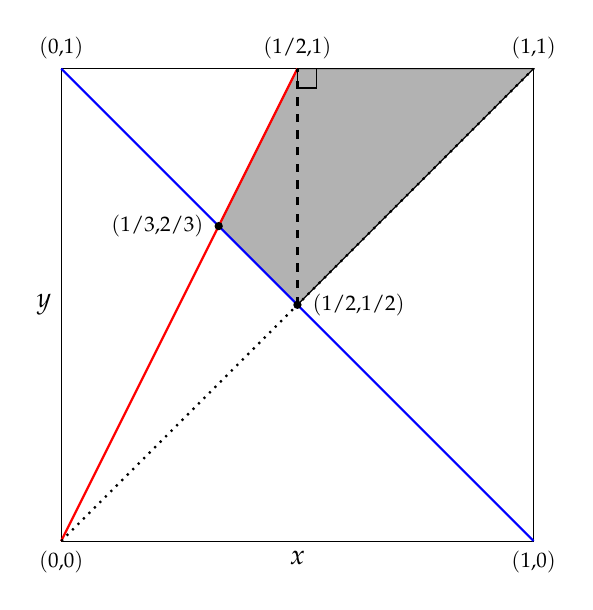
\begin{tikzpicture}[scale=1]
\draw (-3,-3) rectangle +(6,6);
\path (-3,-3) node[below] {$\scriptstyle (0,0)$} --
  node[below] {$x$} (3,-3)
  node[below] {$\scriptstyle (1,0)$};
\path (-3,-3) -- node[left] {$y$} (-3,3)
  node[above] {$\scriptstyle (0,1)$};
\coordinate (P) at (-1,1);
\coordinate (Q) at (0,0);
\draw[fill=white!70!black] (3,3) -- (Q) -- 
  (P) -- (0,3) -- cycle;
\draw[red,thick]  (-3,-3) -- (0,3);
\draw[blue,thick] (-3,3)  -- (3,-3);
\fill (P) circle[radius=1.5pt]
  node[left,xshift=-2pt] {$\scriptstyle (1/3,2/3)$};
\draw[thick,dotted] (-3,-3) -- (3,3);
\fill (Q) circle[radius=1.5pt]
  node[right,xshift=2pt] {$\scriptstyle (1/2,1/2)$};
\node[above] at(0,3) {$\scriptstyle (1/2,1)$};
\node[above] at(3,3) {$\scriptstyle (1,1)$};
\draw[thick,dashed] (Q) -- ++(0,3);
\draw (0,3cm-7pt) rectangle +(7pt,7pt);
\end{tikzpicture}
}
\end{figure}

\ans{2}
כדי שהחלק השמאלי יהיה הארוך ביותר 
$x>y-x$
ו-%
$x>1-y$, 
ולכן
$(x,y)$
חייבת להיות לימינו של
$y=2x$
(אדום) ולימינו של
$y=1-x$
(כחול) (איור%
~\ref{f.shaded2}).
בנוסף, לפי הנחה ש-%
$x$
נמצא לשמאלו של
$y$,
$(x,y)$
חייבת להיות לשמאלו של
$y=x$
(מנוקד).

כדי להקל על החישוב נחלק את האיזור האפור לשני משולשים (מקווקו) ונחשב את התוחלת בנפרד בשניהם. השטח של האיזור האפור מתקבל כסכום השטחים של המשולשים
$1/24+1/8=1/6$.
מכאן:
\begin{eqn}
E(\textrm{השמאלי במשולש}\;x)&=& 6\int_{1/3}^{1/2} x [2x-(1-x)]\,dx  \\
&=&\int_{1/3}^{1/2} \left(18x^2-6x\right)\,dx\\
&=&\left. (6x^3-3x^2)\right|_{1/3}^{1/2}=\disfrac{1}{9}\\
E(\textrm{הימני במשולש}\;x)&=& 6\int_{1/2}^{1} x [1-x]\,dx\\
&=&\int_{1/2}^{1} (6x-6x^2)\,dx\\
&=&\left. \left(3x^2-2x^3\right)\right|_{1/2}^{1}= \disfrac{1}{2}\\
E(x)&=& \disfrac{1}{9}+\disfrac{1}{2} = \disfrac{11}{18}\approx 0.6111\,.
\end{eqn}

התוחלת של אורכו של החלק הבינוני היא
$1-\frac{2}{18}-\frac{11}{18}=\frac{5}{18}\approx 0.2778$.

\textbf{סימולציה}
\selectlanguage{english}
\begin{verbatim}
Expectations: shortest = 0.1111, middle = 0.2778, longest = 0.6111
Averages:     shortest = 0.1115, middle = 0.2783, longest = 0.6102
\end{verbatim}
\selectlanguage{hebrew}

%%%%%%%%%%%%%%%%%%%%%%%%%%%%%%%%%%%%%%%%%%%%%%%%%%%%%%%%%%%%%%%%

\begin{prob}{לנצח במשחק לא-הוגן}{D,S}{(Winning an unfair game)}

נתון מטבע לא-הוגנת שההסתברות לעץ היא 
$1/3 < p < 1/2$. 
הטל את המטבע מספר זוגי של פעמים
$N=2n$.
אתה מנצח אם ורק אם 
\textbf{ביותר}
ממחצית ההטלטת מופיע עץ.

\que{1}
פתח נוסחה עבור ההסתברות לנצח 
$P_N$
ונוסחה עבור ההסתברות לתיקו
$T_N$.

\que{2}
פתח נוסחה עבור ה-%
$N$
עבורו יש את ההסתברות הגבוהה ביותר לנצח.

\textbf{רמז:} 
אם ההסתברות הגבוהה ביותר לנצח היא ב-%
$N$
הטלות אזי 
$P_{N-2} \leq P_N$
ו-%
$P_N\geq P_{N+2}$.
\end{prob}

\solution{}

\ans{1} 
כדי לנצח, עץ חייב להופיע ב-%
$i\in\{n+1, n+2, \ldots, 2n-1, 2n=N\}$
הטלות. מההתפלגות הבינומית:
\begin{eqn}
P_N &=& \sum_{i=n+1}^{2n} \dischoose{2n}{i} p^i (1-p)^{2n-i}\\
T_N &=& \dischoose{2n}{n} p^n (1-p)^{n}\,.
\end{eqn}

\ans{2}
כדי שההסתברות הגבוהה ביותר תהיהעבור
$N=2n$
חייב להתקיים:
\[
P_{2n-2} \leq P_{2n} \quad \textrm{ו-} \quad P_{2n}\geq P_{2n+2}\,.
\]
מתי
$P_{2n-2}\not = P_{2n}$?

\textbf{מקרה 1:}
לאחר הטלה
$2n-2$,
עץ הופיע 
$n$
פעמים ופלי
$n-2$
פעמים (כך שהיית זוכה אם היית עוצר כאן), אבל פלי מופיע בשתי ההטלות הבאות. עכשיו יש
$n$
עץ ו-%
$n$
פלי ולכן אתה מפסיד. ההסתברות היא:
\[
\dischoose{2n-2}{n}p^n(1-p)^{n-2} (1-p)^2\,.
\]

\textbf{מקרה $2$:}
לאחר הטלה
$2n-2$,
עץ הופיע 
$n-1$
פעמים ופלי
$n-1$
פעמים (כך שהיית מפסיד אם היית עוצר כאן), אבל עץ מופיע בשתי ההטלות הבאות. עכשיו יש
$n+1$
עץ ו-%
$n-1$
פלי ולכן אתה מנצח. ההסתברות היא:
\[
\dischoose{2n-2}{n-1}p^{n-1}(1-p)^{n-1} p^2\,.
\]
כדי לאמת את
$P_{2n-2}\leq P_{2n}$,
$P_{2n-2}$
לא יכול לגדול כאשר 
$P_{2n}$
נשאר ללא שינוי (מקרה $1$), אבל 
$P_{2n}$
יכול לגבול עד שהיא גבוהה מ-%
$P_{2n-2}$ (מקרה 2).
לכן:
\begin{eqn}
\dischoose{2n-2}{n}p^n(1-p)^{n-2} (1-p)^2 &\leq&
\dischoose{2n-2}{n-1}p^{n-1}(1-p)^{n-1} p^2\\
\disfrac{1}{n} (1-p) &\leq& \disfrac{1}{n-1} p\\
(n-1)(1-p) &\leq& np\\
n &\leq& \disfrac{1-p}{1-2p}\\
2n &\leq& \disfrac{1}{1-2p}+1\,.
\end{eqn}
באופן דומה, כדי לאמת את
$P_{2n}\geq P_{2n+2}$
חייב להיול ש:
\begin{eqn}
\dischoose{2n}{n+1}p^{n+1}(1-p)^{n-1}  (1-p)^2 &\geq&
\dischoose{2n}{n}p^{n}(1-p)^{n}  p^2\\
\disfrac{1}{n+1} (1-p) &\geq& \disfrac{1}{n} p\\
n(1-p)&\geq& (n+1)p\\
n &\geq& \disfrac{p}{1-2p}\\
2n &\geq&\disfrac{1}{1-2p}-1\,.
\end{eqn}
לכן, ערך עבור
$N=2n$
שעבורו מתקבל ההסתברות הגבוהה ביותר הוא המספר השלם הזוגי הקרוב ביותר ל-%
$1/(1-2p)$.
הקורא מוזמן להראות שאם
$1/(1-2p)$
אי-זוגי אזי
$P_{2n}=P_{2n+2}$.

\textbf{סימולציה}
\selectlanguage{english}
\begin{verbatim}
For probability             = 0.3700
Optimal games to be played  = 4
For  2 games, average won   = 0.1372
For  4 games, average won   = 0.1445
For  6 games, average won   = 0.1431

For probability             = 0.4000
Optimal games to be played  = 6
For  4 games, average won   = 0.1820
For  6 games, average won   = 0.1845
For  8 games, average won   = 0.1680

For probability             = 0.4500
Optimal games to be played  = 10
For  8 games, average won   = 0.2671
For 10 games, average won   = 0.2646
For 12 games, average won   = 0.2640
\end{verbatim}
\selectlanguage{hebrew}

%%%%%%%%%%%%%%%%%%%%%%%%%%%%%%%%%%%%%%%%%%%%%%%%%%%%%%%%%%%%%%%%

\begin{prob}{ממוצע של מספר ההתאמות}{S}{(Average number of matches)}
סדר חפיסת קלפים בשורה בסדר הסטנדרטי ואז סדר חפיסה שניה שורה בסדר אקראי מתחת לשורה הראשונה (איור%
~\ref{f.cards}).
מה התוחלת של מספר ההתאמות של קלף בשורה הראשונה עם קלף בשורה מתחתיו?
\end{prob}

\begin{figure}[tb]
\begin{center}
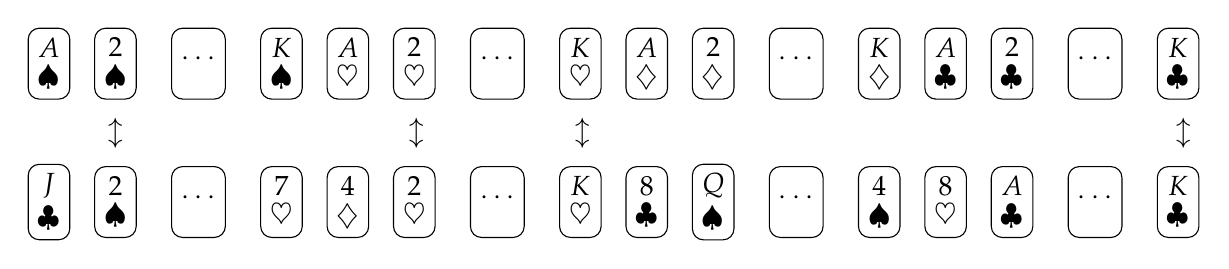
\begin{tikzpicture}
\foreach \x/\v/\s in {
  0/A/\spadesuit,
  1/2/\spadesuit,
  2.25/\cdots/,
  3.5/K/\spadesuit,
  4.5/A/\heartsuit,
  5.5/2/\heartsuit,
  6.75/\cdots/,
  8/K/\heartsuit,
  9/A/\diamondsuit,
  10/2/\diamondsuit,
  11.25/\cdots/,
  12.5/K/\diamondsuit,
  13.5/A/\clubsuit,
  14.5/2/\clubsuit,
  15.75/\cdots/,
  17/K/\clubsuit}
  \node[minimum height=9mm,draw,rounded corners]
    at (\x*24pt,0) {\shortstack{$\v$\\$\s$}};

\foreach \x/\v/\s in {
  0/J/\clubsuit,
  1/2/\spadesuit,
  2.25/\cdots/,
  3.5/7/\heartsuit,
  4.5/4/\diamondsuit,
  5.5/2/\heartsuit,
  6.75/\cdots/,
  8/K/\heartsuit,
  9/8/\clubsuit,
  10/Q/\spadesuit,
  11.25/\cdots/,
  12.5/4/\spadesuit,
  13.5/8/\heartsuit,
  14.5/A/\clubsuit,
  15.75/\cdots/,
  17/K/\clubsuit}
  \node[minimum height=9mm,draw,rounded corners]
    at (\x*24pt,-50pt) {\shortstack{$\v$\\$\s$}};

\node at (24pt,-25pt) {$\updownarrow$};
\node at (133pt,-25pt) {$\updownarrow$};
\node at (193pt,-25pt) {$\updownarrow$};
\node at (410pt,-25pt) {$\updownarrow$};
\end{tikzpicture}
\end{center}
\caption{התאמת שתי חפיסות קלפים}\label{f.cards}
\end{figure}

\solution{}

ההתפלגות אחידה כי לכל קלף בשורה השניה אותה המסתברות להתאים לקלף מעליו. לכן:
\[
E(\textrm{ההתאמות מספר}) = 52\cdot \frac{1}{52} = 1\,.
\]
\selectlanguage{english}
\begin{verbatim}
Expectation of matches = 1.00
Average of matches     = 1.01
\end{verbatim}
\selectlanguage{hebrew}

%%%%%%%%%%%%%%%%%%%%%%%%%%%%%%%%%%%%%%%%%%%%%%%%%%%%%%%%%%%%%%%%

\begin{prob}{הסתברויות של התאמות}{S}{(Probabilities of matches)}

סדר חפיסת קלפים בשורה בסדר הסטנדרטי ואז סדר חפיסה שניה שורה בסדר אקראי מתחת לשורה הראשונה (איור%
~\ref{f.cards}).
פתח נוסחה עבור 
$P(n,r)$,
ההסתברות שיהיו בדיוק 
$r$
התאמות של קלף בשורה הראשונה עם קלף בשורה מתחתיו? הנח ש-%
$P(k,0)$
נתון עבור
$0\leq k\leq n$.
\end{prob}

\solution{}

במבט ראשון נראה שבעיה זו דומה לבעיה~28 אבל קיים הבדל מהותי. השליפות המקופסאות הן בלתי-תלויות אבל כאן ההתאמות תלויות אחת בשניה. למשל, אם יש התאמה בקלף הראשון (בהסתברות 
$1/n$),
ההסתברות של התאמה בקלף השני היא
$1/(n-1)$.

ההסתברות שקבוצה 
\textbf{נתונה}
של
$r$
קלפים מתאימות היא:
\begin{equation}\label{eq.r-match}
\disfrac{1}{n}\cdot \disfrac{1}{n-1}\cdot \cdots \cdot \disfrac{1}{n+r-1}\,.
\end{equation}
כדי לקבל בדיוק 
$r$
התאמות, יש להכפיל משוואה%
~\ref{eq.r-match}
ב-%
$P(n-r,0)$,
ההסתברות שאין בכלל התאמות בשאר 
$n-r$
הקלפים. לבסוף, יש 
${n\choose r}$
דרכים לבחור
$r$
התאמות, ולכן:
\begin{eqn}
P(n,r)&=& \dischoose{n}{r}\disfrac{1}{n(n-1)(n+r-1)} P(n-r,0)\\
&=& \disfrac{n!}{r!(n-r)!}\cdot\disfrac{1}{n!/(n-r)!}P(n-r,0)\\
&=&\disfrac{1}{r!}P(n-r,0)\,.
\end{eqn}
נוסחה זו פותרת את הבעיה כי 
$P(k,0)$
נתונה.

\L{Mosteller}
מפתח נוסחה סגורה וגבול עבור
$P(n,r)$:
{
\addtolength{\arraycolsep}{-3pt}
\begin{eqnarray}
P(n,k)&=&\disfrac{1}{k!}\sum_{i=0}^{n-k} \disfrac{(-1)^i}{i!}\\
\label{eq.r-matches-lim}
\lim_{n-r\rightarrow \infty} P(n,k)&\approx& \disfrac{1}{k!}e^{-1}\,.
\end{eqnarray}
}

\textbf{סימולציה}

הרצתי את הסימולציה עבור 
$n=52$
קלפים וחישבתי את ההסתברות ממשוואה%
~\ref{eq.r-matches-lim}.
\selectlanguage{english}
\begin{verbatim}
Probability of 1 matches = 0.3679
Proportion 1 matches     = 0.3710
Probability of 2 matches = 0.1839
Proportion 2 matches     = 0.1828
Probability of 3 matches = 0.0613
Proportion 3 matches     = 0.0569
Probability of 4 matches = 0.0153
Proportion 4 matches     = 0.0168
\end{verbatim}
\selectlanguage{hebrew}

%%%%%%%%%%%%%%%%%%%%%%%%%%%%%%%%%%%%%%%%%%%%%%%%%%%%%%%%%%%%%%%%

\begin{prob}{לבחור את הנדוניה הגדול ביותר}{D,S}{(Choosing the largest dowry)}

הנח סידרה של 
$n$
קלפים עם הפנים למטה. על פניו של כל קלף נמצא מספר שלם חיובי אבל אין מידע על ההתלפגות שלהם. הפוך את הקלפים אחד-אחד ועיין במספרים. לאחר חשיפת כל אחד מהקלפים, אתה יכול להכריז שמספר זה הוא הגדול ביותר בסידרה. אם אתה צודק אתה מנצח, אחרת אתה מפסיד. למשל, אם הסדרה היא 
$(47, 23, 55, 4)$,
אתה מנצח רק אם אתה בוחר שת הקלף השלישי.

הנה אסטרטגיה: ל-%
$r$
קבוע, וותר על
$r-1$
הקלפים הראשונים ובחר את הקלף הראשון שמספרו גדול מכל 
$r-1$
הקלפים.

\que{1}
עבור
$n=4$
ו-%
$r=3$
בדוק את כל התמורות ומצא בכמה מהם את מנצח.

\que{2}
פתח נוסחה עבור ההסתברות לניצחון עבור 
$n, r$
שרירותיים.

\que{3} מצא קירוב להסתברות כאשר 
$n,r\rightarrow \infty$.

\textbf{רמז:}
נתון
$r$
באיזה מקומות יכול להופיע המספר הגדול ביותר
$m$
ובאיזה מקומות המספרים שהם פחות או שווים ל-%
$m$? 

\end{prob}

\solution{}

\ans{1}
כדי לפשט את הסימון נכתוב את דירוג מספרים כ-%
$1,2,3,4$
למרות שהערכים אמיתיים של המספרים לא ידועים, ולמשל יכולים להיות 
$4,23,47,55$.
אם אתה חושף קלפים
$1,2,3$
(שהם בעצם
$4,23,47$),
אינך יודע אם לבחור
$47$
או לחכות ובחור את הקלף האחרון.

יש 
$24$
תמורות של ארבעה מספרים. לפי האסטרטגיה אתה מוותר על שני הקלפים הראשונים ובוחר או את הקלף השלישי או את הקלף הרביעי, כך שאתה מפסיד אם $4$ נמצא במקום הראשון של התמורה. מה עם התמורה
$(1,2,3,4)$?
אתה מוותר על
$1,2$
ובוחר 
$3$
בגלל שהוא גובהה יותר מ-%
$1,2$
אבל אתה מפסיד כי זה לא המספר הגדולה ביותר. מה עם התמורה
$(1,3,2,4)$?
שוב, לפי האסטרטגיה אתה מוותר על
$1,3$,
אבל מוותר גם על
$2$
כי הוא 
\textbf{לא}
גדול יותר מ-%
$1,3$.
כעת אתה בוחר
$4$
ומנצח. נסח טיעונים דומים לכל התמורות ובדוק שכל התמורות עם 
$4$
במסגרת הן נצחונות:
\[
\addtolength{\arraycolsep}{-2pt}
\renewcommand*{\arraystretch}{1.5}
\begin{array}{cc|cc@{\hspace{2em}}cc|cc@{\hspace{2em}}cc|cc@{\hspace{2em}}cc|cc@{\hspace{2em}}cc|cc@{\hspace{2em}}cc|cc}
1&2\;&\;3&4&
1&2\;&\;\fbox{$4$}&3&
1&3\;&\;2&\fbox{$4$}&
1&3\;&\;\fbox{$4$}&2&
1&4\;&\;2&3&
1&4\;&\;3&2\\
2&1\;&\;3&4&
2&1\;&\;\fbox{$4$}&3&
2&3\;&\;1&\fbox{$4$}&
2&3\;&\;\fbox{$4$}&1&
2&4\;&\;1&3&
2&4\;&\;3&1\\
3&1\;&\;2&\fbox{$4$}&
3&1\;&\;\fbox{$4$}&2&
3&2\;&\;1&\fbox{$4$}&
3&2\;&\;\fbox{$4$}&1&
3&4\;&\;2&1&
3&4\;&\;2&1\\
4&1\;&\;2&3&
4&1\;&\;3&2&
4&2\;&\;1&3&
4&2\;&\;3&1&
4&3\;&\;1&2&
4&3\;&\;2&1
\end{array}
\]
ההסתברות לנצח היא
$10/24$.

\ans{2}
אתה מפסיד אם המספר הגדול ביותר נמצא באחד המקומות
$1,\ldots,r-1$.
לכן כדי לנצח מספר הגדול ביותר חייב להיות במקום
$m$
כאשר
$r\leq m\leq n$:
\[
1\quad 2\quad \cdots\quad r-2 \quad r-1 \quad \overbrace{r \quad r+1 \quad \cdots\quad m-1\quad  m \quad m+1\quad \cdots \quad n}^{\textrm{כאן להיות חייב ביותר גדול מספר}}\,.
\]
לפי האסטרטגיה אתה מוותר על
$r-1$
הקלפים הראשונים. אתה תבחר מקום
$m$
אם ורק אם 
\textbf{כל}
במספרים ב-%
$(r,\ldots,m-1)$
קטנים מ%
\textbf{כל}
המספרים ב-%
$(1,\ldots,r)$.
במילים אחרות, המספר הגדול ביותר בסידרה
$(1,\ldots,m-1)$
הוא
\textbf{לא}
בחלק השני של הסידרה
$(r,\ldots m-1)$
אלא בחלק הראשון
$(1,\ldots,r-1)$.
ההסתברות היא:
\[
P((1,\ldots,r-1)\textrm{ב- נמצא}\;(1,\ldots,m-1)\textrm{ב- ביותר הגדול המספר}) = \disfrac{r-1}{m-1}\,.
\]
ההסתברות שהמספר הגדול ביותר נמצא ב-%
$m$
הוא
$1/n$
ולכן:
\begin{equation}\label{eq.dowry1}
P(\textrm{ניצחון}) = \sum_{m=r}^{n} \disfrac{1}{n} \cdot \disfrac{r-1}{m-1}= \disfrac{r-1}{n}\sum_{m=r}^{n} \disfrac{1}{m-1}\,.
\end{equation}
עבור
$n=4, r=3$, $P(\textrm{ניצחון}) = 5/12=10/24$.

משוואה%
~\ref{eq.dowry1}
לא מוגדרת עבור
$r=1$
אבל ההסתברות לנצח כאשר אתה בוחר את המספר הראשון הוא
$1/n$.
לערך גבוהה ביותר של
$r$
יש הסתברות גבוהה יותר כפי שראינו בדוגמה.

\ans{3}
נכתוב משוואה%
~\ref{eq.dowry1}
כך:
\begin{equation}\label{eq.dowry2}
P(\textrm{ניצחון}) =\disfrac{r-1}{n}\left(\sum_{m=2}^{n} \disfrac{1}{m-1}-\sum_{m=2}^{r-1} \disfrac{1}{m-1}\right)\,.
\end{equation}
עבור 
$n,r$
גדולים, ניתן למצוא קירוב למשוואה%
~\ref{eq.dowry2}
כך:
\[
P(\textrm{ניצחון})=\disfrac{r}{n}(\ln n - \ln r)=\disfrac{r}{n}\ln \disfrac{n}{r}=-\disfrac{r}{n}\ln \disfrac{r}{n}\,.
\]
נסמן
$x=r/n$
ונמצא את המקסימום מהנגזרת:
\begin{eqn}
(-x\ln x)' &=& -x\cdot \frac{1}{x} + (-1) \ln x=0\\
\ln x &=& -1\\
x &=& 1/e\,.
\end{eqn}
כדי למקסם את ההסתברות לנצח בחר
$r \approx n/e$.

\textbf{סימולציה}

הרצתי את הסימולציה עם
$100$
קלפים וערכי
$r$
קרובים ל-%
$100/e$:
\selectlanguage{english}
\begin{verbatim}
Reject cards before r = 36:
Probability of wins   = 0.3674
Proportion wins       = 0.3641
Reject cards before r = 37:
Probability of wins   = 0.3678
Proportion wins       = 0.3759
Reject cards before r = 38:
Probability of wins   = 0.3679
Proportion wins       = 0.3548
Reject cards before r = 30:
Probability of wins   = 0.3590
Proportion wins       = 0.3601
\end{verbatim}
\selectlanguage{hebrew}

%%%%%%%%%%%%%%%%%%%%%%%%%%%%%%%%%%%%%%%%%%%%%%%%%%%%%%%%%%%%%%%%

\begin{prob}{בחירת המספר האקראי הגדול ביותר}{D,S}{(Choosing the largest random number)}

הנח סידרה של 
$n$
קלפים עם הפנים למטה. על פניו של כל קלף נמצא מספר ממשי עם התפלגות אחידה ב-%
$0.0\leq x<1.0$.
הפוך את הקלפים אחד-אחד ועיין במספרים. לאחר חשיפת כל אחד מהקלפים, אתה יכול להכריז שמספר זה הוא הגדול ביותר בסידרה. אם אתה צודק אתה מנצח, אחרת אתה מפסיד.

השתמש באסטרטגיה של בעיה~37: החלט על ערך
$r$
כך שאתה מוותר על 
$r-1$
הקלפים הראשונים ובוחר את הקלף הראשון שגדול מהמספר הגדול ביותר ב-%
$r-1$
קלפים הראשונים.

\textbf{הגדרה:}
$d$,
\textbf{ערך שווה-נפש},
הוא הערך שמתחתיו אתה מוותר על הקלף ומעליו את לבחור את הקלף.

\que{1} 
חשב את
$d$
עבור
$n=1$
וחשב את ההסתברות לנצח.

\que{2}
חשב את
$d$
עבור
$n=2$
וחשב את ההסתברות לנצח.

\que{3}
חשב את
$d$
עבור
$n=3$.
אל תנסה לחשב את ההסתברות לנצח!

\textbf{הערה:}
בבעיה~37 בערכים יכולים להיות
$100, 200, 300$ 
או
$100, 50, 20$
כך שחשיפת המספר הראשון לא מספק שום מידע על המספרים האחרים. בבעיה זו, ההתלפגות אחידה, ולכן אם המספר הראשון הוא 
$0.2$,
ההסתברות שהמספר השני יהיה גדול יותר היא 
$0.8$
ואם המספר הראשון הוא 
$0.8$
ההסתברות שהמספר השני יהיה גדול יותר היא
$0.2$.

\end{prob}

\solution{}

יהי
$v_1,v_2,v_3$
המספרים על שלושת הכרטיסים.

\ans{1}
אין ברירה אלא לבחור את הקלף הראשון כי אין קלפים אחרים. לכן אין ערך שווה-נפש. 
$v_1$
הוא המספר "הגדול ביותר",
$P({ניצחון})=1$.

\ans{2}
אם אתה בוחר את הקלף הראשון
$P(\textrm{ניצחון})=v_1$
שהיא ההסתברות שהמספר על הקלף השני קטן יותר. אם אתה מוותר על הקלף הראשון,
$P(\textrm{ניצחון})=1-v_1$
שהיא ההסתברות ש-%
$v_2>v_1$.
לכן, אם 
$v_1<0.5$ 
בחר את הקלף השני כי
$1-v_1>0.5$
ואם 
$v_1>0.5$
בחר את הקלף הראשון. מכאן ש-%
$d=0.5$.

הנה הנוסחה לחישוב ההסתברות לנצח:
\[
P(\textrm{ניצחון}) = p(\textrm{ניצחון} \,|\,v_1<0.5)\,p(v_1<0.5)+ p(\textrm{ניצחון}\,|\,v_1>0.5)\,p(v_1>0.5)\,.
\]
$p(v_1<0.5)=0.5$
נובע מההתפלגות האחידה. מה עם
$p(\textrm{ניצחון} \,|\,v_1<0.5)$? 
לפי האסטרטגיה אתה מנצח אם
$0.5<v_2<1$
אבל גם אם
$v_1<v_2<0.5$.
ההתפלגות של 
$v_1$
היא אחידה ב-%
$(0,0.5)$
ולכן:
\[
p(\textrm{ניצחון} \,|\,v_1<0.5)=\disfrac{1}{2} + \disfrac{1}{4}=\disfrac{3}{4}\,.
\]
ניתן לעשות חישוב דומה עבור
$v_1>0.5$.
נרכיב את כל החישובים הללו ביחד וקבל:
\[
P(\textrm{ניצחון})=\disfrac{3}{4}\cdot\disfrac{1}{2}+\disfrac{3}{4}\cdot\disfrac{1}{2}=\disfrac{3}{4}\,.
\]

\ans{3}
אם אתה בוחר את הקלף הראשון,
$P(\textrm{ניצחון})=v_1^2$
כי הקלף השני והשלישי חייבים להיות קטנים מהראשון.

אם אתה מוותר על הקלף הראשון ובוחר את השני כי 
$v_2>v_1$
אזי:
\begin{itemize}
\item $P(\textrm{ניצחון})=(1-v_1)v_1$
אם
$v_2>v_1$ 
ו-%
$v_3<v_1$.
\item $P(\textrm{ניצחון})=v_1(1-v_1)$
אם
$v_2<v_1$
ו-%
$v_3>v_1$.
\item $P(\textrm{ניצחון})=\frac{1}{2}(1-v_1)^2$
אם
$v_2>v_1$
ו-%
$v_3>v_1$,
כי ניצחון תלוי בסדר:
\\
אם הוא
$(0.55, 0.75, 0.65)$
אתה מנצח
ואם הוא
$(0.55, 0.65, 0.75)$
אתה מפסיד.
\end{itemize}

הערך שווה-נפש 
$d$
הוא ערך עבורו ההסתברות לנצח על ידי בחירת הקלף הראשון שווה להסתברות לנצח על ידי ויתור על הקלף הראשון:
\begin{eqn}
d^2 &=& 2d(1-d) + \frac{1}{2}(1-d)^2\\
5d^2 - 2d -1 &=&0\\
d&=& \disfrac{1+\sqrt{6}}{5}\approx 0.6899\,.
\end{eqn}
\L{Gilbert\&Mosteller} \cite[page~55]{gilbert}
מראים שעבור
$n=3$:
\[
P(\textrm{ניצחון}) = \disfrac{1}{3}+\disfrac{d}{2}+\disfrac{d^2}{1}-\disfrac{3d^3}{2}\approx 0.6617\,.
\]
\textbf{סימולציה}
\selectlanguage{english}
\begin{verbatim}
For  3 cards:
Indifference value = 0.6000
Probability of win = 0.6693
Proportion of wins = 0.6628
Indifference value = 0.6899
Probability of win = 0.6617
Proportion of wins = 0.6711
Indifference value = 0.7200
Probability of win = 0.6519
Proportion of wins = 0.6473
\end{verbatim}
\selectlanguage{hebrew}

%%%%%%%%%%%%%%%%%%%%%%%%%%%%%%%%%%%%%%%%%%%%%%%%%%%%%%%%%%%%%%%%

%% !TeX root = mos-he.tex

%%%%%%%%%%%%%%%%%%%%%%%%%%%%%%%%%%%%%%%%%%%%%%%%%%%%%%%%%%%%%%%%

\begin{prob}{להכפיל את הדיוק}{}{(Doubling your accuracy)}

נתון שני מקלות באורכים
$L_1<L_2$
ומכשיר למדידת מרחק ששגיאת המדידה שלו ניתן על ידי התפלגות נורמלית עם ממוצע
$0$
ושונות
$\sigma^2$.
ניתן למדוד את אורכי המקלות על ידי מדידת כל מקל בנפרד. האם יש דרך מדוייקת יותר?
\end{prob}
\solution{}

\begin{figure}[bt]
\begin{center}
\begin{tikzpicture}
\draw (0,0) -- ++(6,0) -- ++(0,12pt) -- ++(-6,0) -- cycle;
\draw[<->] (0,24pt) --
  node[fill=white] {$\scriptstyle L_1+L_2$} ++(14,0);
\draw (6,0) -- ++(8,0) -- ++(0,12pt) -- ++(-8,0) -- cycle;
\begin{scope}[yshift=-48pt]
\draw (0,0) -- ++(8,0) -- ++(0,12pt) -- ++(-8,0) -- cycle;
\draw[yshift=12pt] (0,0) -- ++(0,12pt) -- ++(6,0) -- ++(0,-12pt);
\draw[<->] (6,20pt) --
  node[fill=white] {$\scriptstyle L_2-L_1$} ++(2,0);
\end{scope}
\end{tikzpicture}
\end{center}
\caption{מדידת האורכים של שני מקלות}\label{f.rods}
\end{figure}
הנח את המקלות קצה לקצה ומדד
$L_s=L_1+L_2$,
ואחר כך הנח את המקלות צד לצד ומדד
$L_d=L_2-L_1$ (איור%
~\ref{f.rods}).
חשב
$L_1,L_2$:
\begin{eqn}
\textstyle\frac{1}{2}(L_s-L_d)=\frac{1}{2}((L_1+L_2)-(L_2-L_1))&=&L_1\\
\textstyle\frac{1}{2}(L_s+L_d)=\frac{1}{2}((L_1+L_2)+(L_2-L_1))&=&L_2\,.
\end{eqn}
השגיאות במדידות הן
$e_s, e_d$
כך שהשגיאות התוצאות הן:
\begin{eqn}
\textstyle\frac{1}{2}((L_s+e_s)-(L_d+e_d))&=&L_1+\textstyle\frac{1}{2}(e_s-e_d)\\
\textstyle\frac{1}{2}((L_s+e_s)+(L_d+e_d))&=&L_2+\textstyle\frac{1}{2}(e_s+e_d)\,.
\end{eqn}
ממוצע של השגיאות במכשיר הוא
$0$
ולכן הממוצע של שתי המדידות גם כן $0$. השונות יורדת למחצית ערכה הקודמת:%
\footnote{%
המדידות בלתי-תלויות ולכן הקווריאנס הוא $0$.}
\begin{eqn}
\mathrm{Var}\left(\textstyle\frac{1}{2}\left(e_s-e_d\right)\right)&=&
  \textstyle\frac{1}{4}(\sigma^2+(-1)^2\sigma^2)=\frac{1}{2}\sigma^2\\
\mathrm{Var}\left(\textstyle\frac{1}{2}(e_s+e_d)\right)&=&
  \textstyle\frac{1}{4}( \sigma^2+\sigma^2)=\frac{1}{2}\sigma^2\,.
\end{eqn}


%%%%%%%%%%%%%%%%%%%%%%%%%%%%%%%%%%%%%%%%%%%%%%%%%%%%%%%%%%%%%%%%

\begin{prob}{משוואות ריבועיות אקראיות}{S}{(Random quadratic equations)}

תהי 
$x^2+2bx+c=0$
משוואה ריבועית המוגדרת מעל
$[-B,B]\times[-B,B]$
עבור
$B\geq 1$.

\que{1}
מה ההסתברות שהשורשים ממשיים?

\que{2} 
כאשר 
$B\rightarrow \infty$
מה ההסתברות שהשורשים ממשיים?
\end{prob}
\solution{}

\ans{1}
השורשים יהיו ממשיים אם הדיסקרימיננט 
$4b^2-4c\geq 0$
לא-שלילי. איור%
~\ref{f.real-roots}
מראה גרף של הפרבולה
$c=b^2$
כאשר השורשים המרוכבים נמצא בשטח האפור. למשל, עבור
$(b,c)=(1,2)$, 
ל-%
$x^2+2x+2$
שורשים מרוכבים (נקודה אדומה) ועבור
$(b,c)=(2,2)$
ל-%
$x^2+4x+2$
שורשים ממשיים (נקודה כחולה).

\begin{figure}[tb]
\begin{center}
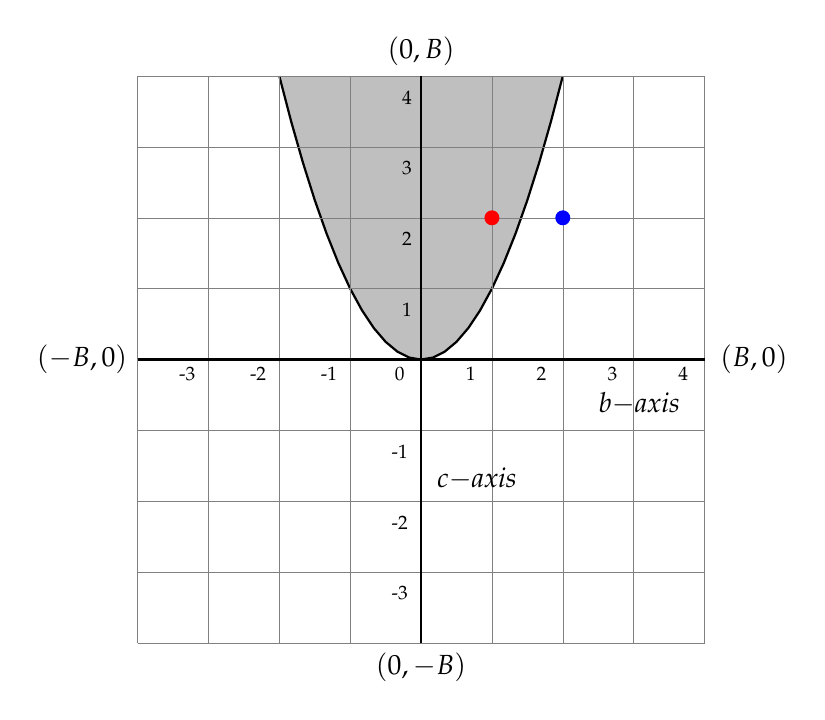
\begin{tikzpicture}[scale=.9]
\fill [white!50!gray, domain=-2:2]
      (-2, 4) -- plot ({\x}, {\x*\x}) -- (2, 4) -- cycle;
\draw [thick, domain=-2:2]
      (-2, 4) -- plot ({\x}, {\x*\x}) -- (2, 4);
\draw[help lines] (-4,-4) grid (4,4);
\draw[thick] (-4,0) -- (4,0);
\draw[thick] (0,-4) -- (0,4);
\foreach \x in {-3,...,4}
  \node at (\x-.3,-.2) {\scriptsize \x};
\foreach \y in {1,...,4}
  \node at (-.2,\y-.3) {\scriptsize \y};
\foreach \y in {-3,...,-1}
  \node at (-.3,\y-.3) {\scriptsize \y};
\draw[thick] (0,-4) node[below] {$(0,-B)$} -- 
  node[right,near start,xshift=2pt,yshift=8pt]
  {$c\mathit{-axis}$} (0,4) node[above] {$(0,B)$};
\draw[thick] (-4,0) node[left] {$(-B,0)$} --
  node[below,very near end,xshift=2pt,yshift=-8pt] 
  {$b\mathit{-axis}$} (4,0) node[right,xshift=2pt] {$(B,0)$};
\fill[red] (1,2) circle(3pt);
\fill[blue] (2,2) circle(3pt);
\end{tikzpicture}
\end{center}
\caption{%
עבור 
$(b,c)$
בשטח האפור השורשים של
$c=b^2$
מרוכבים}
\label{f.real-roots}
\end{figure}

נחשב את השטח האפור על ידי אינטגרציה:
\[
\int_{-\sqrt{B}}^{\sqrt{B}} (B-b^2)\,db=
\left. Bb-\disfrac{b^3}{3}\right|_{-\sqrt{B}}^{\sqrt{B}}=
\left(B^{3/2}-\frac{B^{3/2}}{3}\right)-
\left(-B^{3/2}+\frac{B^{3/2}}{3}\right)=
\disfrac{4}{3}B^{3/2}\,.
\]
השטח הכולל של
$[-B,B]\times[-B,B]$
הוא
$4B^2$
ולכן:
\begin{eqn}
P(\textrm{מרוכבים שורשים})&=&\disfrac{\frac{4}{3}B^{3/2}}{4B^2}=\disfrac{1}{3\sqrt{B}}\\
P(\textrm{ממשיים שורשים})&=&1-\disfrac{1}{3\sqrt{B}}\,.
\end{eqn}
\ans{2}
\[
\lim_{B\rightarrow\infty}
P(\textrm{ממשיים שורשים})=
\lim_{B\rightarrow\infty} \left(1-\disfrac{1}{3\sqrt{B}}\right)=
1\,.
\]

\textbf{סימולציה}
\selectlanguage{english}
\begin{verbatim}
For B =  4:
Probability of real roots = 0.8333
Proportion real roots     = 0.8271
For B = 16:
Probability of real roots = 0.9167
Proportion real roots     = 0.9205
For B = 64:
Probability of real roots = 0.9583
Proportion real roots     = 0.9582
\end{verbatim}
\selectlanguage{hebrew}

%%%%%%%%%%%%%%%%%%%%%%%%%%%%%%%%%%%%%%%%%%%%%%%%%%%%%%%%%%%%%%%%

\begin{prob}{הילוך מקרי דו-ממדי}{S}{(Two-dimensional random walk)}

חלקיק נמצא במרכז של מערכת צירים דו-ממדית. החלקיק צועד ימינה או שמאלה על ציר ה-%
$x$
עם הסתברות 
$1/2$
לכל כיוון 
\textbf{ובו-זמנית}
צועד למעלה או למטה על ציר ה-%
$y$
עם הסתברות 
$1/2$
לכל כיוון. איור%
~\ref{f.2d-random-walk}
מראה הילוך מקרי של 
$22$
צעדים שמתחיל ונגמר במרכז.

\que{1}
מה ההסתברות שהחלקיק חוזר למרכז ב-$2$ צעדים?

\que{2}
פתח נוסחה עבור ההתסתברות שהחלקיק חוזר למרכז (פעם אחת או יותר).

\que{3}
השתמש בקירוב של
\L{Stirling}
כדי לקבל הערכה של ההסתברות עבור $n$ גדול.

\begin{figure}[t]
\begin{center}
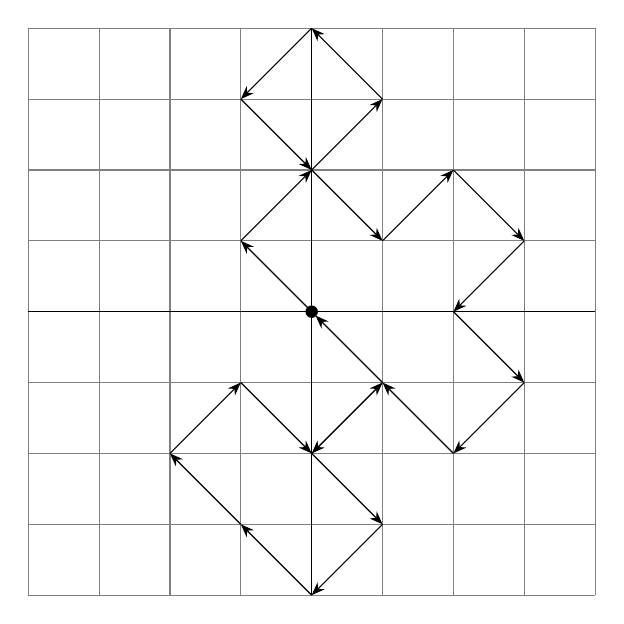
\begin{tikzpicture}[scale=.9]
\draw[color=gray] (-4,-4) grid (4,4);
\draw (-4,0) -- (4,0);
\draw (0,-4) -- (0,4);
\fill (0,0) circle[radius=2.5pt];
\draw[->] (0,0)  -- (-1,1);
\draw[->] (-1,1) -- (0,2);
\draw[->] (0,2)  -- (1,3);
\draw[->] (1,3)  -- (0,4);
\draw[->] (0,4)  -- (-1,3);
\draw[->] (-1,3) -- (0,2);
\draw[->] (0,2)  -- (1,1);
\draw[->] (1,1)  -- (2,2);
\draw[->] (2,2)  -- (3,1);
\draw[->] (3,1)  -- (2,0);
\draw[->] (2,0)  -- (3,-1);
\draw[->] (3,-1) -- (2,-2);
\draw[->] (2,-2) -- (1,-1);
\draw[->] (1,-1) -- (0,-2);
\draw[->] (0,-2) -- (1,-3);
\draw[->] (1,-3) -- (0,-4);
\draw[->] (0,-4) -- (-1,-3);
\draw[->] (-1,-3)-- (-2,-2);
\draw[->] (-2,-2)-- (-1,-1);
\draw[->] (-1,-1)-- (0,-2);
\draw[->] (0,-2) -- (1,-1);
\draw[->] (1,-1) -- (.055,-.055);
\end{tikzpicture}
\end{center}
\caption{הילוך מקרי דו-ממדי}\label{f.2d-random-walk}
\end{figure}
\end{prob}
\solution{}

\ans{1}
הנקודות באיור%
~\ref{f.two-moves}
מראות את המקומות האפשריים בהם החלקיק יכול להיות לאחר שני צעדים:
\begin{itemize}
\item
המסלול הירוק מראה איך להגיע ל-%
$(\pm 2, \pm 2)$
על ידי שני צעדים באותו כיוון. ההסתברות היא
$\left(\frac{1}{4}\right)^2= \frac{1}{16}$.
\item
המסלול האדום מראה איך להגיע ל-%
$(\pm 2,0)$
או ל-%
$(0,\pm 2$).
יש שני מסלולים אפשריים לכל נקודה ולכן ההסתברות היא
$2\cdot\left(\frac{1}{4}\right)^2= \frac{2}{16}$.
\item
המסלול הכחול מראה איך להגיע ל-%
$(\pm 1,\pm 1)$
ולחזור למרכז. ההסבתרות היא
$1/16$.
יש ארבעה מסלולים שחוזרים למרכז ולכן ההסתברות היא
$\frac{4}{16}$.
\end{itemize}
רק המסלולים הכחולים חוזרים למרכז ולכן:
\[
P(\textrm{צעדים בשני למרכז חזרה})=\frac{4}{16}\,.
\]

\begin{figure}[tb]
\begin{center}
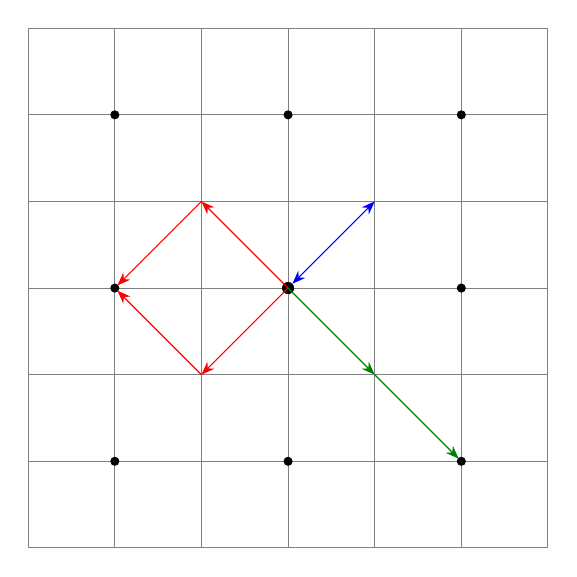
\begin{tikzpicture}[scale=1.1]
\draw[color=gray] (-3,-3) grid (3,3);
\fill (0,0) circle[radius=2pt];
\foreach \x/\y in {2/2, 2/-2, -2/2, -2/-2, 
                   0/2, 0/-2, 2/0, -2/0}
  \fill (\x,\y) circle[radius=1.5pt];
\draw[->,red] (0,0) -- (-1,-1);
\draw[->,red] (-1,-1) -- (-1.97,-.03);
\draw[<-,red] (-1.97,0.03) -- (-1,1);
\draw[<-,red] (-1,1) -- (0,0);
\draw[->,green!50!black] (0,0) -- (1,-1);
\draw[->,green!50!black] (1,-1) -- (1.97,-1.97);
\draw[<->,blue] (.05,.05) -- +(.95,.95);
%\draw[->,blue] (-0.1,0) -- +(1,1);
%\draw[->,blue] (1.1,1) -- +(-1,-1);
\end{tikzpicture}
\end{center}
\caption{שני צעדים בהילוך מקרי}\label{f.two-moves}
\end{figure}

\ans{3}
בחירת הכיוון בשני מצירים היא בלתי-תלויה כך שעבור
$2n$
צעדים:
\begin{equation}\label{eq.2d-1}
P_{2n}(\textrm{למרכז חזרה}) =
P_{2n}(x\!=\!0\textrm{ל- חזרה})\,P_{2n}(y\!=\!0\textrm{ל- חזרה})\,.
\end{equation}
החלקיק יחזור למרכז אם ורק אם בשני הצירים מספר הצעדים 
$+1$
שווה המספר צעדים
$-1$.
יש 
${2n \choose n}$
דרכים לסדר
$+1$
ו-%
$-1$
ולכן:
{
\addtolength{\arraycolsep}{-3pt}
\begin{eqnarray}
P_{2n}(x\!=\!0\textrm{ל- חזרה}) =P_{2n}(y\!=\!0\textrm{ל- חזרה})&=&
\dischoose{2n}{n}\left(\disfrac{1}{2}\right)^n\left(\disfrac{1}{2}\right)^{n}\\
P_{2n}(\textrm{למרכז חזרה}) &=&
\left[\dischoose{2n}{n}\left(\disfrac{1}{2}\right)^{2n}\right]^2\\
P(\textrm{למרכז חזרה}) =
\sum_{n=1}^{\infty}P_{2n}(\textrm{למרכז חזרה}) &=&
\sum_{n=1}^{\infty}\left[\dischoose{2n}{n}\left(\disfrac{1}{2}\right)^{2n}\right]^2\,.\label{eq.2d-2}
\end{eqnarray}
}
\ans{3}
לפי הקירוב של
\L{Stirling}
$n! \approx \sqrt{2\pi n}\left(n/e\right)^n$:
\begin{eqn}
P_{2n}(\textrm{למרכז חזרה}) &=&
\left[\dischoose{2n}{n}
\left(\disfrac{1}{2}\right)^{2n}\right]^2 \\
&=&
\left[\disfrac{(2n)!}{(n!)^2}
\left(\disfrac{1}{2}\right)^{2n}\right]^2 \\
&\approx&
\left(\disfrac{1}{2}\right)^{4n}
\disfrac{(\sqrt{2\pi \cdot 2n})^2
         \left(2n/e\right)^{4n}}
        {(\sqrt{2\pi n})^{4}
         \left(n/e\right)^{4n}} \\
&=&\left(\disfrac{1}{2}\right)^{4n}\disfrac{4\pi n}{4\pi^2 n^2}\cdot
\disfrac{\left(n/e\right)^{4n}\cdot 2^{4n}}{\left(n/e\right)^{4n}}\\
&=& \disfrac{1}{\pi n}\\
P(\textrm{למרכז חזרה}) &=& \disfrac{1}{\pi}\sum_{n=1}^{\infty}\disfrac{1}{n}\,,
\end{eqn}
שהיא
\textbf{סידרה הרמונית}
שמתבדרת, כלומר, עם הסתברות 
$1$
החלקיק חוזר למרכז!

\textbf{סימולציה}
הרצתי את הסימולציה מיליון פעמים במקום עשרת אלפים פעמים אבל התוצאה לא מראה שהחלקיק מגיע למרכז בוואדות.
\selectlanguage{english}
\begin{verbatim}
Proportion returned to origin      = 0.8700
\end{verbatim}
\selectlanguage{hebrew}

%%%%%%%%%%%%%%%%%%%%%%%%%%%%%%%%%%%%%%%%%%%%%%%%%%%%%%%%%%%%%%%%

\begin{prob}{הילוך מקרי תלת-ממדי}{D,S}{(Three-dimensional random walk)}

לקיק נמצא במרכז של מערכת צירים תלת-ממדית. החלקיק צועד ימינה או שמאלה על ציר ה-%
$x$
עם הסתברות 
$1/2$
לכל כיוון 
\textbf{ובו-זמנית}
צועד למעלה או למטה על ציר ה-%
$y$
עם הסתברות 
$1/2$
לכל כיוון.
\textbf{ובו-זמנית}
צועד פנימה או החוצה על ציר ה-%
$z$
עם הסתברות 
$1/2$
לכל כיוון.

\que{1}
מה
\textbf{התוחלת}
של מספר הפעמים שהחלקיק חוזר למרכז?

\textbf{רמז:}
חשב את ההסתברות ואחר כך תשתמש במשתנה מסמן
\L{(indicator variable)}.

\que{2}
מה ההסתברות שהחלקיק יחזור למרכז לפחות פעם אחת?

\textbf{רמז:}
תשתשמש בשיטה של בעיה~4.
\end{prob}
\solution{}

$P_{2n}$,
ההסתברות לחזור למרכז לאחר
$2n$
נתון על ידי הכללת משוואה%
~\ref{eq.2d-1}
לשלושה ממדים:
\[
P_{2n} =
P_{2n}(x=0\textrm{ל- חוזר})\,P_{2n}(y=0\textrm{ל- חוזר}\, P_{2n}(z=0\textrm{ל- חוזר})\,.
\]
$P_r$,
ההסתברות לחזור למרכז לפחות פעם אחת ניתנת על ידי הכללה לשלושה ממדים של משוואה%
~\ref{eq.2d-2}:
\[
P_r =\sum_{n=1}^{\infty}P_{2n} =
\sum_{n=1}^{\infty}\left[\dischoose{2n}{n}\left(\disfrac{1}{2}\right)^{2n}\right]^3\,.
\]
מהקירוב של
\L{Stirling}:\footnote{\L{Mosteller}
השתמש ב-%
$18$
איברים בחישוב שלו וקיבל
$0.315$.
התכנית שלי השתמש ב-%
$500$
איברים וקיבלתי
$0.3772$.}
\begin{eqn}
P_{2n} &=&
\left[\disfrac{(2n)!}{(n!)^2}
\left(\disfrac{1}{2}\right)^{2n}\right]^3 \\
&\approx&
\left(\disfrac{1}{2}\right)^{6n}
\disfrac{(\sqrt{2\pi \cdot 2n})^3
         \left(2n/e\right)^{6n}}
        {(\sqrt{2\pi n})^{6}
         \left(n/e\right)^{6n}} \\
&=&\disfrac{(4\pi n)^{3/2}}{(2\pi n)^3}=
 \disfrac{1}{(\pi n)^{3/2}}\\
P_r &=& \sum_{n=1}^{\infty}\disfrac{1}{(\pi n)^{3/2}}\approx 0.3772\,.
\end{eqn}
יהי 
$I_k$
משתנה מסמן עבור חזרה למרכז בצעד
$k$:
\begin{equation}
I_k=
\left\{
\begin{array}{ll}
1,\quad k\;\textrm{בצעד למרכז חוזר החלקיק אם}\\
0, \quad k\;\textrm{בצעד למרכז חוזר לא החלקיק אם}\,.
\end{array}
\right.
\end{equation}
אזי:
\[
E(\textrm{למרכז החזרות מספר})=\sum_{n=1}^{\infty}P_{2n}\, I_{2n} = P_r\approx 0.3772\,,
\]
ולכן התוחלת למספר החזרות למרכז שווה להסתברות.

\que{2}
תהי
$P_1$
ההסתברות שהחלקיק חוזר למרכז
\textbf{לפחות פעם אחת}.
מבעיה~4 אנו יודעים שהתוחלת של מספר בניסויים עד מראשון בו החלקיק 
\textbf{לא}
חוזר למרכז היא
$1/(1-P_1)$.
לכן, התוחלת של מספר הניסויים עד שהחליק כן חוזר למרכז היא אחד פחות, כי החלקיק יכול לחזור למרכז מספר רב של פעמים עד שהוא לא חוזר.%
\footnote{%
קשה לעקוב אחר הצגת הדברים של
\L{Mosteller}.
ברצוני להודית ל-%
\L{Aaron Montgomery}
שהבהיר לי את הפתרון
\L{\cite{montgomery}}.}

תהי
$E_r=E(\textrm{למרכז החזרות מספר})$. 
אזי:
\begin{eqn}
E_r &=& \disfrac{1}{1-P_1} - 1\\
P_1&=& \disfrac{E_r}{1+E_r}\,.
\end{eqn}
ב-%
\ansnc{1}
חישבנו ש-%
$E_r\approx 0.3772$
ולכן:
\[
P_1 \approx 1- \disfrac{1}{1+0.3772}
\approx 0.2739\,.
\]

\textbf{סימולציה}
\selectlanguage{english}
\begin{verbatim}
Expectation of reaching origin = 0.3772
Average times reached origin   = 0.3630
Probability of reaching origin = 0.2739
Proportion reached origin      = 0.2790
\end{verbatim}
\selectlanguage{hebrew}

%%%%%%%%%%%%%%%%%%%%%%%%%%%%%%%%%%%%%%%%%%%%%%%%%%%%%%%%%%%%%%%%

\begin{prob}{המחט של \L{Buffon}}{D,S}{(Buffon's needle)}

נתון משטח עם קווים מקביליים במרחק 
$1$
אחד מהשני. קח מחט באורך 
$a\leq 1$
וזרוק אותו על המשטח. מה ההסתברות שהמחט חוצה קו?%
\footnote{%
כדי להקל על החישובים אנו מניחים שהמרחק בין הקווים הוא 
$1$.
ניתן להתעלם מאפשרות שהמחט שוכב כולו לאורך אחד הקווים וכן את האפשרות שהוא נודע בשני קווים כי ההתסברות של אירועים אלה היא אפס.}

\textbf{רמז:}
יש שני משתנים אקראיים (איור%
~\ref{f.buffon1}): 
$x$,
המקום של מרכז המחט ביחס לקו הקרוב ביותר עם התפלגות אחידה בטווח 
$[0,1/2]$,
ו-%
$\theta$, 
הזווית שבין המחט לבין הקווים המקביליים עם התפלגות אחידה בטווח 
$[0,\pi/2]$.

\begin{figure}[tb]
\begin{center}
\begin{tikzpicture}[scale=.9]
\draw (0,0) -- (10,0);
\draw (0,4) -- (10,4);
\draw[<->] (1,0) -- node[fill=white] {$1$} (1,4);
\coordinate (center) at ($(4,-.5)+(60:1.5)$);
\node[above right,xshift=4pt] at (center) {$\theta$};
\node[above left] at (center) {$C$};
\draw[thick] (4,-.5) -- node[right,very near end] {$a$} +(60:4);
\draw[thick,dashed] ($(center)+(-2,0)$) -- +(6,0);
\draw[<->] (5.3,0) -- node[fill=white] {$x$}
  (center -| 5.3,0);
\end{tikzpicture}
\end{center}
\caption{המחט של\;Buffon}\label{f.buffon1}
\end{figure}
\end{prob}
\solution{1}

תהי 
$p(a)$
ההסתברות שמחט באורך 
$a$
חוצה קו והגדר משתנה מסמן:
\[
I_{\textrm{קו חוצה}}=
\left\{
\begin{array}{ll}
1,\quad \textrm{קו חוצה}\;a\;\textrm{באורך מחט}\\
0,\quad \textrm{קו לא חוצה}\;a\;\textrm{באורך מחט}\,.
\end{array}
\right.
\]
אזי:
\begin{equation}\label{eq.buffon-probability}
E(I_{\textrm{קו חוצה}})=1\cdot p(a) + 0\cdot (1-p(a))=p(a)\,,
\end{equation}
וניתן לחשב את ההסתברות על ידי חישוב התוחלת.

יהי 
$m$
אנח לקווים המקביליים שעובר דרך מרכז המחט ותהי 
$\theta$
הזווית בין המחט לבין אחד מהקווים המקביליים. הטל את המחט על 
$m$
כדי לקבל את הקטע הקו
$\overline{CD}$
(איור%
~\ref{f.buffon2}).
ההסתברות שהמחט חוצה קו היא:
\begin{equation}\label{eq.cross}
P(\textrm{קו חוצה}\;\theta\;\textrm{וזווית}\;a\;\textrm{באורך מחט})=\disfrac{(a/2)\sin \theta}{1/2}=a\sin\theta\,.
\end{equation}

\begin{figure}[bt]
\begin{center}
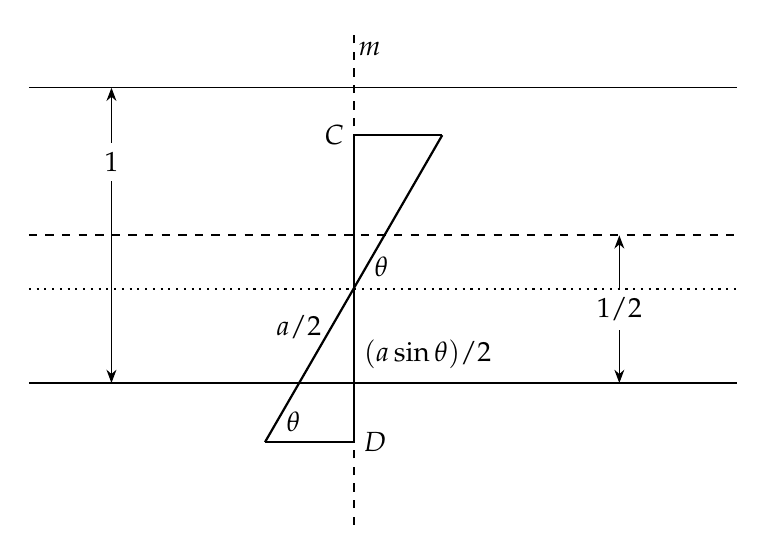
\begin{tikzpicture}[scale=1.5]
\draw (0,0) coordinate (O) -- (6,0);
\draw (0,2.5) -- (6,2.5);
\draw[<->] (.7,0) -- node[fill=white,near end] {$1$} +(0,2.5);
\draw[<->] (5,0) -- node[fill=white] {$1/2$} +(0,1.25);
\coordinate (end1) at (2,-.5);
\coordinate (end2) at ($(end1)+(60:3)$);
\coordinate (center) at ($(end1)+(60:1.5)$);
\draw[thick,dotted] (O |- center) -- +(6,0);
\draw[thick,dashed] (0,1.25) -- +(6,0);
\node[right,xshift=4pt,yshift=8pt]
  at (center) {$\theta$};
%\node[left,xshift=-4pt,yshift=-8pt]
%  at (center) {$\theta$};
\draw[thick,dashed] ($(center)+(0,-2)$) --
  node[right,very near end,xshift=-2pt,yshift=15pt]
  {$m$} +(0,4.2);
\node[right] at (end1 -| center) {$D$};
\node[left] at (end2-| center) {$C$};
\draw[thick] (end1) -- 
  node[left,near end] {$a/2$} (center) --
%  node[right] {$a/2$} 
  (end2);
\draw[thick] (end1) node[above right,xshift=4pt] {$\theta$} --
  (end1 -| center) --
  node[right,yshift=4pt] {$(a\sin\theta)/2$} (center);
\draw[thick] (end2) -- (end2 -| center) -- (center);
%\draw[thick] (end2) node[below left,xshift=-4pt] {$\theta$} --
%  (end2 -| center) -- 
%  node[left] {$(a\sin \theta)/2$} (center);
\end{tikzpicture}
\end{center}
\caption{משולש ישר-זווית לפתרון בעיית המחט של \L{Buffon}}
\label{f.buffon2}
\end{figure}

התוחלת של מספר הקווים שהמחט חוצה מתקבלת על ידי אינטגרציה מעל לזוויות האפשריות:
\begin{equation}\label{eq.buffon-integral}
E(\textrm{lines crossed}) =
  \disfrac{1}{(\pi/2)-0} \int_0^{\pi/2} a\sin \theta\,
  d\theta=\left.\disfrac{2}{\pi}\cdot a (-\cos \theta)
  \right|_0^{\pi/2}=\disfrac{2a}{\pi}\,.
\end{equation}

\solution{2}
הפתרון מבוסס על
\L{\cite[Chapter~26]{proofs}}.

\begin{figure}[tb]
\begin{center}
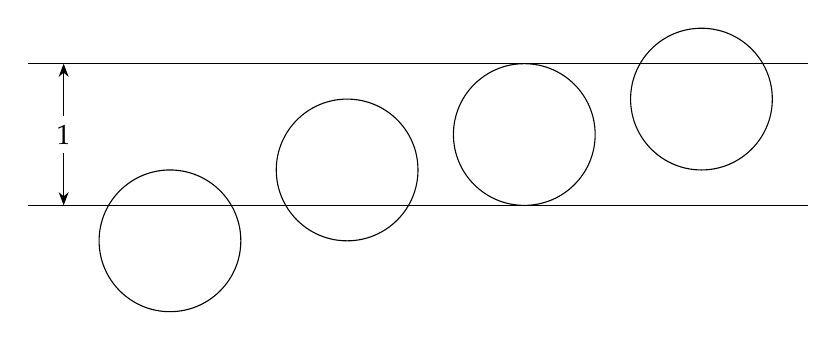
\begin{tikzpicture}[scale=.9]
\draw (0,0) -- (11,0);
\draw (0,2) -- (11,2);
\draw[<->] (.5,0) -- node[fill=white] {$1$} (.5,2);
\foreach \x/\y in {2/-.5, 4.5/.5, 7/1, 9.5/1.5}
  \draw (\x,\y) circle[radius=1];
\end{tikzpicture}
\end{center}
\caption{%
הפתרון של בעיית המחט של Buffon על מעגלים}
\label{f.buffon3}
\end{figure}

תהי 
$E(x)$
התוחלת שמ מספר הקווים המקביליים שקו באורך
$x$
חוצה. עיין עכשיו בקו שמסובבים למעגל
$C$
\textbf{בקוטר}
$1$
והיקף
$\pi$.
אם תזרוק את המעגל על המשטח, הוא יחצה קו 
\textbf{בדיוק}
פעמיים (איור%
~\ref{f.buffon3}),
ולכן:
\begin{equation}\label{eq.buffon-2}
E(C)=2\,.
\end{equation}
בנה מצולע משוכלל
$Q_n$
חסום על ידי 
$c$
(אדום), ובנה מצולע משוכלל 
$R_n$
שחוסם את
$c$
(כחול) (איור%
~\ref{f.buffon4}). 
כל קו ש-%
$Q_n$
חוצה (אדום) חייב לחצות את המעגל וכל קו שחוצה את המעגל (כחול) חייב לחצות את 
$R_n$.
לכן:
\begin{equation}\label{eq.buffon3}
E(Q_n)\leq E(C)\leq E(R_n)\,.
\end{equation}
יהי 
$a_Q, a_R$
סכומי באורכים של צלעות של
$Q_n,R_n$,
בהתאמה. לפי הליניאריות של התוחלת:
{
\addtolength{\arraycolsep}{-3pt}
\begin{eqnarray}\label{eq.buffon1a}
E(Q_n)&=&\sum_{i=1}^n E(a_Q\;\textrm{של צלעות})=a_QE(1)\\
\label{eq.buffon1b}E(R_n)&=&\sum_{i=1}^n E(a_R\;\textrm{של צלעות})=a_RE(1)\,. 
\end{eqnarray}
}
כאשר 
$n\rightarrow\infty$
שני המצולעים הם קירובים למעגל ולכן:
\begin{equation}\label{eq.buffon-pi}
\lim_{n\rightarrow\infty}a_Q = \lim_{n\rightarrow\infty} a_R=\pi\,,
\end{equation}
ההיקף של המעגל. ממשוואות%
~\ref{eq.buffon-2}--\ref{eq.buffon-pi}
מתקבל:
\[
\renewcommand*{\arraystretch}{1.5}
\begin{array}{l}
\lim_{n\rightarrow\infty}E(Q_n)=E(C) =\lim_{n\rightarrow\infty}E(R_n)\\
E(C)=aE(1) =\pi E(1) = 2\\
E(1)=\disfrac{2}{\pi}\\
E(a)=aE(1)=\disfrac{2a}{\pi}\,.
\end{array}
\]
\begin{figure}[bt]
\begin{center}
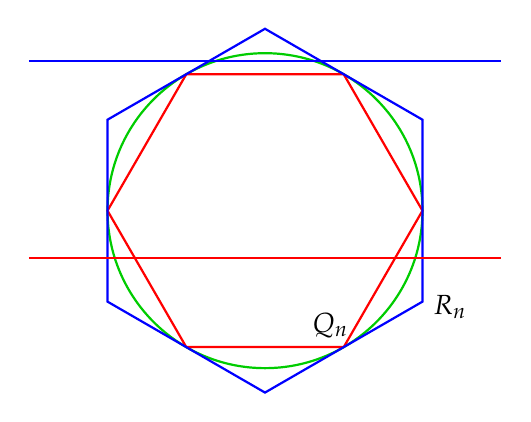
\begin{tikzpicture}
\draw[thick,green!80!black] (0,0) circle[radius=2];
\node[draw,red,thick] (in)
  [minimum size=4cm,regular polygon,regular polygon sides=6]
  at (0,0) {};
\node[draw,blue,rotate=30,thick] (out)
  [minimum size=4.62cm,regular polygon,regular polygon sides=6]
  at (0,0) {};
\node[above left,xshift=5pt] at (in.corner 5) {$Q_n$};
\node[below right,yshift=6pt] at (out.corner 5) {$R_n$};
\draw[thick,red] (-3,-.6) -- +(6,0);
\draw[thick,blue] (-3,1.9) -- +(6,0);
\end{tikzpicture}
\end{center}
\caption{מצולעים כקירובים למעדל}\label{f.buffon4}
\end{figure}

\textbf{סימולציה}

$\pi=2a/E$
ולכן ניתן לחשב קירוב לערכו על ידי הרצת סימולציה או זריקת מחטים על שולחן!
\selectlanguage{english}
\begin{verbatim}
For length = 0.2:
Expectation of crossings = 0.1273
Average crossings        = 0.1308
Empirical value for pi   = 3.0581

For length = 0.5:
Expectation of crossings = 0.3183
Average crossings        = 0.3227
Empirical value for pi   = 3.0989

For length = 1.0:
Expectation of crossings = 0.6366
Average crossings        = 0.6333
Empirical value for pi   = 3.1581
\end{verbatim}
\selectlanguage{hebrew}

%%%%%%%%%%%%%%%%%%%%%%%%%%%%%%%%%%%%%%%%%%%%%%%%%%%%%%%%%%%%%%%%

\begin{prob}{המחט של \L{Buffon} עם רשת אופקי ואנכי}{}{\\(Buffon's needle with horizontal and vertical rulings)}

פתור את בעיית המחט של 
\L{Buffon}
עבור משטח עם רשת אופקי ואנכי כאשר גודל המשבצות הוא 
$1\times 1$.
מחט יכול לחצות קו אנכי (ירוק), קו אופקי (כחול), שניהם (אדום) או אף אחד (כתום) (איור%
~\ref{f.buffon5}).

\begin{figure}[b]
\begin{center}
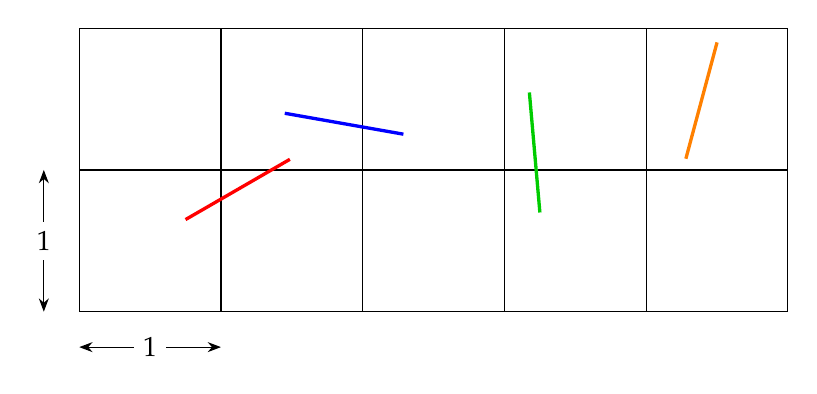
\begin{tikzpicture}[scale=.9]
\draw[step=2cm] (0,0) grid (10,4);
\draw[<->] (-.5,0) -- node[fill=white] {$1$} (-.5,2);
\draw[<->] (0,-.5) -- node[fill=white] {$1$} (2,-.5);
\foreach \x/\y/\a/\c in {
  1.5/1.3/30/red,
  2.9/2.8/-10/blue,
  6.5/1.4/95/green!80!black,
  9/3.8/-105/orange}
    \draw[color=\c,very thick] (\x,\y) -- +(\a:1.7);
\end{tikzpicture}
\end{center}
\caption{בעיית המחט של 
\L{Buffon}
עבור משטח עם רשת אופקי ואנכי}
\label{f.buffon5}
\end{figure}
\end{prob}
\textbf{רמז:}
האם מספר הקווים האופקים והאכנים שהמחט חוצה בלתי-תלויים?

\solution{}

מספר הקווים האופקים והאכנים שהמחט חוצה אכן בלתי-תלויים, ולפי הליניאריות של התוחלת:
\begin{eqn}
E(\textrm{חוצה}\; a\;\textrm{באורך שמחט קווים})&=&
E(\textrm{חוצה}\; a\;\textrm{באורך שמחט אנכים קווים}+\\
&&\quad\; \textrm{\textrm{חוצה}\; a\;\textrm{באורך שמחט אופקים קווים}})\\
&&E(\textrm{חוצה}\; a\;\textrm{באורך שמחט אנכים קווים})+\\
&&E(\textrm{\textrm{חוצה}\; a\;\textrm{באורך שמחט אופקים קווים}})\\
&=&\disfrac{2a}{\pi}+\disfrac{2a}{\pi}=\disfrac{4a}{\pi}\,.
\end{eqn}


%%%%%%%%%%%%%%%%%%%%%%%%%%%%%%%%%%%%%%%%%%%%%%%%%%%%%%%%%%%%%%%%

\begin{prob}{מחטים ארוכים}{D,S}{(Long needles)}

יהי 
$a>1$
אורכו של המחט בבעייתו של
\L{Buffon}.

\que{1}
מה התוחלת של
\textbf{מספר הקווים}
שמחט חוצה?

\que{2} 
מה ההסתברות שהמחט חוצה
\textbf{לפחות}
קו אחד?

\textbf{רמז:}
עבור איזו זוויות 
$\theta$
ההסתברות של חציית קו היא
$1$?

\end{prob}
\solution{}

\ans{1}
שבור את המחט לחלקים באורים
$\{a_1,a_2,\ldots, a_n\}$, $a_i< 1$,
כך ש-%
$\sum_{i=1}^n a_i=a$.
לפי הליניאריות של התוחלת והפתרון של בעיה~53:
\[
E(a)= \sum_{i=1}^n E(a_i)= \disfrac{2a}{\pi}\,.
\]

\ans{2}
הפתרון מבוסס על
\L{\cite{wiki-buffon}}
ו-%
\L{\cite[Chapter~26]{proofs}}.

לפי משוואה%
~\ref{eq.cross}
ההסתברות שהמחט יחצה קו היא
$a\sin\theta$ 
\textbf{אם}
$a\sin\theta \leq 1$,
כלומר, אם
$0\leq\theta\leq\sin^{-1}(1/a)$.
אבל, אם
$a\sin\theta > 1$
ההסתברות היא
$1$
(איור%
~\ref{f.buffon6}).
נכליל את משוואה%
~\ref{eq.buffon-integral}
עבור
$a>0$
שרירותי. האינטגרל מוחשב בשני חלקים, אחד עבור
$\theta<\sin^{-1}(1/a))$
ואחר עבור
$\theta>\sin^{-1}(1/a))$:
\begin{eqn}
E(a) &=& \disfrac{2}{\pi}
   \left(\int_{0}^{\sin^{-1}(1/a)} 
   a\sin \theta\:d\theta + 
   \int_{\sin^{-1}(1/a)}^{\pi/2} 1\: d\theta\right)\\
&=& \disfrac{2}{\pi}\left(\left.
    a(-\cos \theta)\right|_0^{\sin^{-1}(1/a)} + 
    \left(\disfrac{\pi}{2} - 
    \sin^{-1}(1/a)\right)\right)\\
&=& 1+\disfrac{2}{\pi}
  \left(a
  \left(1-\sqrt{1-\disfrac{1}{a^2}}\right)-
  \sin^{-1}(1/a)\right)\,.
\end{eqn}

\begin{figure}[tb]
\begin{center}
\begin{tikzpicture}[scale=1]
\draw (0,0) -- (10,0);
\draw (0,3.5) -- (10,3.5);
\draw[<->] (.5,0) -- node[fill=white,near end] {$1$} +(0,3.5);
\draw[<->] (5.5,0) -- node[fill=white] {$1/2$} +(0,1.75);
\begin{scope}[xshift=0cm,yshift=1.4cm,scale=1]
\coordinate (end1) at (2,-1);
\coordinate (end2) at ($(end1)+(60:3)$);
\coordinate (center) at ($(end1)+(60:1.5)$);
\node[above right,xshift=2pt,yshift=-2pt]
  at (end1) {$\theta$};
\draw (end1) --  node[left,near end] {$a/2$} (center) -- (end2);
\draw (end2) -- (end2 -| center);
\draw (end1) -- (end1 -| center);
\draw[very thick] (end1 -| center) -- 
  node[right,fill=white,yshift=2pt] {$(a/2)\sin \theta$}
  (center) -- (end2 -| center);
\draw[thick,dotted] (O |- center) -- +(10,0);
\end{scope}
\begin{scope}[xshift=3cm,yshift=.8cm,scale=1.6]
\coordinate (end1) at (2,-1);
\coordinate (end2) at ($(end1)+(60:3)$);
\coordinate (center) at ($(end1)+(60:1.5)$);
\node[above right,xshift=2pt,yshift=-2pt]
  at (end1) {$\theta$};
\draw (end1) --  node[left,near end] {$a/2$} (center) -- (end2);
\draw (end2) -- (end2 -| center);
\draw (end1) -- (end1 -| center);
\draw[very thick] (end1 -| center) -- 
  node[right,fill=white,yshift=6pt] {$(a/2)\sin \theta$}
  (center) -- (end2 -| center);
\end{scope}
\end{tikzpicture}
\end{center}
\caption{מחטים ארוכים}\label{f.buffon6}
\end{figure}

\textbf{סימולציה}
\selectlanguage{english}
\begin{verbatim}
For length = 1.5:
Expectation of crossings = 0.7786
Average crossings        = 0.7780
For length = 2.0:
Expectation of crossings = 0.8372
Average crossings        = 0.8383
For length = 3.0:
Expectation of crossings = 0.8929
Average crossings        = 0.8897
\end{verbatim}
\selectlanguage{hebrew}

%%%%%%%%%%%%%%%%%%%%%%%%%%%%%%%%%%%%%%%%%%%%%%%%%%%%%%%%%%%%%%%%

\begin{prob}{הכד של \L{Molina}}{}{(Molina's urns)}

שני כדים
$U_1,U_2$
מכילים 
$m$
כדורים כל אחד. ב-%
$U_1$
נמצאים 
$w_1$
כדורים לבנים ו-%
$b_1$
כדורים שחורים, וב-%
$U_2$
נמצאים
$w_2$
כדורים לבנים ו-%
$b_2$
כדורים שחורים. מכל כד שלוף
$n$
כדורים
\textbf{עם החזרה}.

\que{1}
עבור ערכים שונים של
$n>1$
מצא
$w_1,b_1,w_2,b_2$
כך ש:
\[
P(\textrm{לבנים}\;U_1\textrm{מ- שנשלפו כדורים כל})=
P(\textrm{שחורים או לבנים}\;U_2\textrm{מ- שנשלפו כדורים כל})\,.
\]
\end{prob}
\solution{}

\ans{1}
עבור 
$n=2$
המשוואה שיש לפתור היא:
\begin{eqn}
\left(\disfrac{w_1}{m}\right)^2&=&\left(\disfrac{w_2}{m}\right)^2+\left(\disfrac{b_2}{m}\right)^2\\
w_1^2&=&w_2^2+b_2^2\,.
\end{eqn}
פתרון אחד הוא
$w_1=10,b_1=4,w_2=6,b_2=8$.

\ans{2}
לפי המשפט האחרון של
\L{Fermat},
שהוכח ב-%
$1995$
על ידי
\L{Andrew Wiles},
אין פתרונות ל-%
$w_1^n=w_2^n+b_2^n$ 
עבור
$n\geq 3$.

%%%%%%%%%%%%%%%%%%%%%%%%%%%%%%%%%%%%%%%%%%%%%%%%%%%%%%%%%%%%%%%%


%% !TeX root = mos-he.tex

%%%%%%%%%%%%%%%%%%%%%%%%%%%%%%%%%%%%%%%%%%%%%%%%%%%%%%%%%%%%%%%%

\newpage

\begin{center}
\textbf{\LARGE סקירה על הסתברות}
\end{center}
\addcontentsline{toc}{section}{\Large סקירה של הסתברות}

סעיף זה סוקר מושגים בהתסבתרות. אביא דוגמה של כל מושג עבור הטלת קוביה הונגת עם שש פאות. 

\textbf{ניסוי \L{\small (trial)}}
מושג לא מוגדר כאשר הכוונה היא לפעולה שיש לה תוצאות אפשריות.

\textbf{תוצאה \L{\small (outcome)}} 
התוצאה של ניסוי. אם אתה מטיל קוביה אחת תוצאה אפשרית היא 
$4$.

\textbf{מרחב מדגם \L{\small (sample space)}}
קבוצת כל התוצאות האפשריות של ניסוי. הקבוצה 
$S=\{1,2,3,4,5,6\}$
היא מרחב המדגם של הטלת קוביה.

\textbf{אירוע \L{\small (event)}}
תת-קבוצה של מרחב מדגם. תת-הקבוצה 
$e=\{2,4,6\}\subseteq S$
היא האירוע של הופעת מספר זוגי בהטלת קוביה.

\textbf{משתנה אקראי \L{\small (random variable)}}
פונקציה ממרחב המדגם למספרים. יהי 
$T$
מרחב המדגם של של הזוגות (הסדורות) הם התוצאות של הטלת זוג קוביות:
\[
T=\{(a,b)| a,b\in \{1,2,3,4,5,6\} \}\,.
\]
הגדר משתנה אקראי 
$X$
כפונקציה
$X:T \mapsto \{2,3,\ldots,11,12\}$
שממפה תוצאות של הטלת זוג קוביות לסכום המספרים על הקוביות:
\begin{equation}\label{eq.sum}
X((a,b)) = a+b\,.
\end{equation}

\textbf{איחוד, חיתוך, משלים \L{\small (union, intersection, complement)}} 
אירועים הם קבוצות ולכן למושגים הללו יש את המשמעות הרגילה בתורת הקבוצות. יהי
$e_1=\{2,4,6\}$
ו-%
$e_2=\{1,2,3\}$. 
אזי:
\[
e_1 \cup e_2=\{1,2,3,4,6\}\quad e_1 \cap e_2=\{2\}\quad \overline{e_1} = S\setminus e_1=\{1,3,5\}\,.
\]
החיתוך הוא קבוצת המספרים הזוגיים מתוך שלושת האיברים הראשונים במרחב המדגם. המשלים הוא קבוצת המספרים האי-זוגיים מתוך מרחב המדגם.

\textbf{זרים \L{\small (mutually exclusive)}} 
שני אירועים או יותר זרים זה לזה אם החיתוך שלהם הוא הקבוצה הריקה. שני נאירועים
$e_1=\{2,4,6\}$
ו-%
$e_2=\{1,3,5\}$
זרים זה לזה כי
$e_1 \cap e_2=\emptyset$,
כלומר, אין תוצאות שהן מספרים שהם גם זוגיים וגם אי-זוגיים.

\textbf{הסתברות \L{\small (probability)}}
המשמעות האינטואיטיבית של הסתברות היא שהיא הגבול של התדירות היחסית של אירוע. יהי
$e$ 
אירוע ויהי
$n_e$
מספר הפעמים שהאירוע 
$e$
מתרחש ב-%
$n$
חזרות על הניסוי. 
$P(e)$,
ההסתברות של האירוע
$e$,
היא:
\[
P(e) = \lim_{n\rightarrow \infty} \frac{n_e}{n}\,.
\]
הגדרה זו היא בעייתית כי אנחנו לא ממש יודעים אם הגבול קיים. ההגדרה תלויה על "חזרות על הניסוי" אולם אנו רוצים להגדיר הסתברות ללא קשר לסדרה מסוימת של ניסויים. 
\textbf{חוק המספרים הגדולים}
מבטיח שהתפיסה האינטואיטיבית של הסתברות כי תדירות יחסית קרא מאוד למה שקורה כאשר חוזרים על ניסוי מספר רק של פעמים.

התיאוריה המודרנית של הסתברות מבוססת על שלוש אקסיומות שהן די אינטואיטיביות:
\begin{itemize}
\item 
עבור אירוע
$e$, $P(e) \geq 0\,$.
\item 
עבור כל התוצאות האפשריות במרחת 
$S$, $P(S) = 1\,$.
\item
עבור קבוצה של אירועים זה לזה
$\{e_1,\ldots,e_n\}$:
\[
P\left(\bigcup_{i=1}^{n} e_i\right)=\sum_{i=1}^{n} P(e_i)\,.
\]
\end{itemize}

\textbf{החזרה \L{\small (replacement}}
בעיה שכיחה בהסתברות היא לשאול שאלות על שליפת כדור צבעוני מכד. חשוב שהבעיה תציין אם השליפה היא עם או בלי החזרה: לאחר שליפת הכדור האם מחזירים אותו לכד או לא לפני השליפה הבאה? נשלוף שני כדורים מכד עם שלושה כדורים אדומים ושלושה שחורים. לאירוע שהשליפה של הכדור הראשונה שולף כדור אדום הסתברות של
$\frac{3}{3+3}=\frac{1}{2}$.
אם מחזירים את הכדור לפני השליפה השניה אזי ההסתברות שהשליפה של הכדור השני שולף כדור האדום נשארת 
$\frac{1}{2}$
ולכן ההסתברות ששני הכדורים הם אדומים היא
$\frac{1}{4}$.
אם לא מחזירים את הכדור ההסתברות שהכדור השני הוא אדום יורדת ל-%
$\frac{2}{2+3}=\frac{2}{5}$,
ולכן ההסתברות ששני הכדורים הם אדומים היא
$\frac{1}{2}\cdot\frac{2}{5}=\frac{1}{4}$.

\textbf{התפלגות אחידה \L{\small (uniformly distributed)}} 
אם הסתברויות של כל התוצאת במרחב שוות להסתברות התפלגות אחידה. אם 
$S$
היא קבוצה סופית ולהסתברות שלה התפלגות אחידה אזי:
\[
P(e)=\frac{|e|}{|S|}\,.
\]
אם אתה מטיל קוביה
\textbf{הוגנת}
ההסתברות של התוצאות מתפלגת אחידה ולכן עבור
$e=\{2,4,6\}$:
\[
P(e) = \frac{|e|}{|S|} = \frac{|\{2,4,6\}|}{|\{1,2,3,4,5,6\}|}=\frac{1}{2}\,.
\]

\textbf{הסתברות מותנית \L{\small (conditional probability)}} 
יהי 
$e_1,e_2$
אירועים. 
$P(e_1 | e_2)$,
ההסתברות המותנית ש-%
$e_1$
מתרחש אם נתון ש-%
$e_2$
מתרחש, נתונה על ידי:
\[
P(e_1 | e_2) = \disfrac{P(e_1 \cap e_2)}{P(e_2)}\,.
\]
יהי 
$e_1=\{1,2,3\}$
האירוע שקוביה מראה מספר פחות או שווה ל-%
$3$
ויהי
$e_2=\{2,4,6\}$
האירוע שהקוביה מראה מספר זוגי. אזי:
\[
P(e_2 | e_1) = \disfrac{P(E_2 \cap E_1)}{P(e_1)}=\disfrac{P(\{2\})}{P(\{2,4,6\})}= \disfrac{1/6}{1/2}=\disfrac{1}{3}\,.
\]
אם אתה יודע שמספר הוא פחות או שווה ל-%
$3$,
רק אחת משלושת התוצאה היא מספר זוגי.

\textbf{בלתי-תלוי \L{\small (independence)}}
שני אירועים בלתי-תלויים אם ההסתברות של החיתוך שלהם היא המכפלה של ההסתברויות הנפרדות:
\[
P(e_1 \cap e_2)=P(e_1)\,P(e_2)\,.
\]
במונחים של הסבתרות מותנית:
\[
P(e_1 | e_2)=\frac{P(e_1)\cap P(e_2)}{P(e_2)} = \frac{P(e_1)\,P(e_2)}{P(e_2)}=P(e_1)\,. 
\]
עבור אירועים בלתי-תלויים
$e_1,e_2$,
ידיעה של הההסתברות של
$e_2$
לא מספק מידע על ההסתברות של
$e_1$.
שלוש הטלות של קוביה הוגנת בלתי-תלויות ולכן ההסתברות שכולן מראות מספר זוגי היא
$\frac{1}{2}\cdot \frac{1}{2}\cdot \frac{1}{2}=\frac{1}{8}$. 

\textbf{ממוצע \L{\small (average)}}
תהי
$S=\{a_1,\ldots,a_n\}$
קבוצה של ערכים. אזי:
\[
\mathit{Average}(S)=\disfrac{\sum_{i=1}^{n} a_i}{n}\,.
\]
ממוצע מחושב מעל לקבוצה של ערכים אבל הממוצע לא חייב להיות איבר בקבוצה. אם יש
$1000$
משפחות בעיירה ולהן
$3426$
ילדים, הממוצע של מספר הילדים למשפחה היא
$3.426$
למרות שברור שאין משפחה עם
$3.426$
ילדים. אם אתה מטיל קוביה שש פעמים ומקבל את המספרים
$\{2,2,4,4,5,6\}$
הממוצע הוא:
\[
\frac{2+2+4+4+5+6}{6}=\frac{23}{6}\approx 3.8\,,
\]
שוב, לא איבר בקבוצה.

\textbf{תוחלת \L{\small (expectation)}}
התוחלת של משתנה אקראי היא סכום ההסתברויות של כל תוצאה כפול הערך של משתנה האקראי עבור אותה תוצאה. עבור קוביה הוגנת לכל תוצאה יש הסתברות זהה ולכן:
\[
E(\textrm{קוביה ערך})=1\cdot \frac{1}{6} + 2\cdot\frac{1}{6} + 3\cdot\frac{1}{6} + 4\cdot\frac{1}{6} + 5\cdot\frac{1}{6} + 6\cdot\frac{1}{6}=3.5\,.
\]
השתנה האקראי
$X$
ממשוואה%
~\ref{eq.sum}
ממפה את המספרים המופיעים על זוג קוביות לסכום המספרים. ההסתברות של כל זוג היא
$1/36$,
אבל לזוגות
$(2,5)$
ו-%
$(5,2)$
אותו סכום ולכן הם שייכים לאותה תוצאה. הערכים של המשתנה האקראי הם
$\{2,\ldots,12\}$
ומספר הדרכים לקבל כל אחד מהן הם:
\[
\begin{array}{l|rrrrrrrrrrr}
\textrm{סכום} & 2 & 3 & 4 & 5 & 6 & 7 & 8 & 9 & 10 & 11 & 12\\\hline
\textrm{זוגות} & 1 & 2 & 3 & 4 & 5 & 6 & 5 & 4 & 3 & 2 & 1
\end{array}
\]
התוחלת היא הממוצע של ערכי המשתנה האקראי כפול 
\textbf{המשקל}
שהוא ההסתברות של כל תוצאה. יהי
$E_s$
התוחלת של סכום הערכים כאשר מטילים זוג קוביות. אזי:
\begin{equation}\label{eq.two-dice}
E_s=2\cdot \frac{1}{36} + 3\cdot \frac{2}{36} + 4\cdot \frac{3}{36} + 
\cdots + 10\cdot \frac{3}{36} + 11\cdot \frac{2}{36} + 12\cdot \frac{1}{36} = 7\,.
\end{equation}
עבור קבוצה שרירותית של אירועים
$\{e_1,\ldots,e_n\}$
התוחלת היא:
\[
E=\sum_{i=1}^{n} e_iP(e_i)\,.
\]

\textbf{ליניאריות של התוחלת \L{\small (linearity of expectation)}}\label{p.linearity}
נעיין שוב בתוחלת של הסכום של זוג קוביות (משוואה%
~\ref{eq.two-dice}).
תהי 
$E(e_6)$
התוחלת של האירוע שסכום הקוביות הוא
$6$.
אזי:
\[
E(e_6) = X(e_6)P(e_6)=6\cdot \frac{5}{36}\,,
\]
כי יש
$5$
זוגות מתוך 
$36$
הזוגות האפשריים שסכומם 
$6$: $(1,5), (2,4), (3,3), (4,2), (5,1)$.
אבל ניתן לחשב את התוחלת כדלקמן כאשר
$P(i,j)$
היא ההסתברות שהזוג 
$(i,j)$
מופיע ו-%
$E(i,j)$
היא התוחלת של
$i+j$:
\begin{eqn}
E(X(e_6)) &=& 6\cdot P(1,5)+6\cdot P(2,4)+6\cdot P(3,3)+6\cdot P(4,2)+6\cdot P(5,1)\\
&=& (1+5)\cdot \textstyle\frac{1}{36}+(2+4)\cdot \frac{1}{36}+(3+3)\cdot \frac{1}{36}+(4+2)\cdot \frac{1}{36} +(5+1)\frac{1}{36}\\
&=&E(1,5)+E(2,4)+E(3,3)+E(4,2)+E(5,1)\\
&=&\sum_{i,j | i+j=6}E(i,j)\,.
\end{eqn}
החישוב תלוי בעובדה שהאירועים בלתי-תלויים כי ברור ש-%
$(2,4)$
ו-%
$(3,3)$
לא יכולים להופיע באותו ניסוי.

באותה שיטה ניתן להוכיח את ההכללה
(\L{\cite[Section~4.9]{ross}}):
\[
E\left(\sum_{i=1}^{n} a_ie_i\right)=\sum_{i=1}^{n} a_iE(e_i)\,,
\]
שנקראת הליניאריות של התוחלת. במקרה של שני משתנים אקראיים:
\[
E(ae_1 + be_2) = aE(e_1) + bE(e_2)\,.
\]

\textbf{משתנה מסמן \L{\small (indicator variable)}}
יהי
$e$
אירוע שההסתברות שלה היא
$P(e)$.
הגדר
$I_e$,
משתנה מסמן עבור 
$e$,
כך
\L{\cite[Chapter~4, Example~3b]{ross}}:
\[
I_e=
\left\{
\begin{array}{ll}
1,\quad \textrm{מתרחש}\; e\;\textrm{אם}\\
0, \quad \textrm{מתרחש לא}\;e\;\textrm{אם}\,.
\end{array}
\right.
\]
מכאן ש:
\[
E(I_e)=1\cdot P(e) + 0\cdot (1-P(e))=P(e)\,.
\]
ניתן להכליל משוואה זו. נתונה קבוצה של אירועים
$\{e_1,\ldots\}$
והמשתנים המסמנים שלהם
$\{I_1,\ldots\}$:
\begin{equation}\label{eq.expectation-prob}
E\left(\sum_{i=1}^{\infty} I_{i}\right) = \sum_{i=1}^{\infty} I_{i}p(e_i) = \sum_{i=1}^{\infty} (1\cdot p(e_i) + 0\cdot (1-p(e_i)) =\sum_{i=1}^{\infty} p(e_i)\,.
\end{equation}
בנוסף:
\begin{equation}\label{eq.expectation-sum}
\sum_{i=1}^{\infty} E(I_{i})=E\left(\sum_{i=1}^{\infty} I_{i}\right)\,.
\end{equation}
ההוכחה של נוסחה זו קשה והנוסחה תקיפה כאן בגלל שהמשתנים באקראיים לא שליליים.

\textbf{משפט הבינום \L{\small (binomial theorem)}}
אם
$p$
היא ההסתברות של אירוע
$e$
אזי ההסתברות שהתוצאה של סדרה של 
$n$
ניסויים בלתי-תלויים היא
\textbf{בדיוק}
$k$
אירועים 
$e$
ניתנת על ידי
\textbf{המקדם הבינומי (\L{binomial coefficient})}:
\[
\dischoose{n}{k} p^k (1-p)^{n-k}\,.
\]
בהכללה, ההסתברות ש-%
$e$
מתרחוש בין
$i$
ל-%
$j$
פעמים היא:
\[
\sum_{k=i}^{j}\dischoose{n}{k} p^k (1-p)^{n-k}\,.
\]
לפי משפט הבינום:
\begin{eqn}
\sum_{i=0}^{n} \dischoose{n}{i} x^i y^{n-i}&=&(x+y)^n\\
\sum_{i=0}^{n} \dischoose{n}{i} p^i (1-p)^{n-i}&=&(1+(1-p))^n=1\,,
\end{eqn}

כפי שאפשר לצפות כי אחת התוצאות חייבת להתרחש.

\textbf{סכום סדרה הרמונית \L{\small (sum of a harmonic series)}}\label{p.harmonic}
עבור 
$n$
מספר שלם חיובי, הסדרה ההרמונית היא:
\[
H_n=\sum_{k=1}^{n}\disfrac{1}{k}\approx \ln n + \frac{1}{2n} + \gamma\,,
\]
כאשר
$\gamma \approx 0.5772$
הוא
\textbf{הקבוע של \L{Euler} \L{(Euler's constant)}}.
כאשר
$n$
שואף לאינסוף הסדרה מתבדרת:
\[
\sum_{k=1}^{\infty}\disfrac{1}{k}=\infty\,,
\]
כי
$\ln n$
אינו חסום.

\textbf{הקירוב של \L{Stirling} \L{\small (Stirling's approximation)}}
קשה מאוד לחשב
$n!$ 
עבור 
$n$ 
גדול. נוח להשתמש באחת הנוסחאות של הקירוב של
\L{Stirling}:
\begin{eqn}
n! &\approx& \sqrt{2\pi n}\left(\disfrac{n}{e}\right)^n\\
\ln (n!) &\approx& n\ln n - n\\
\ln (n!)  &\approx& n\ln n - n + \frac{1}{6}\left(8n^3+4n^2+n+\frac{1}{30}\right)+\frac{1}{2}\ln\pi\,.
\end{eqn}

\textbf{התפלגות הסתברותית רציפה\L{\small (Continuous probability distribution)}}\label{p.continuous}
התפלגויות הסתברות רציפות בדרך כלל לא מופיעות בספר אבל עבור קוראים עם הרקע המתאים אנו סורקים את המושגים הבסיסיים.

ניתן להגדיר הסתברויות מעל למשתנים אקראים רציפים.  
\textbf{פונקציית הסתברות צפיפות \L{\small (probability density function (PDF))}} $f(x): \mathcal{R}\rightarrow \mathcal{R}$
ממפה תוצאה 
$x$
לערך של הפונקציה וכך להגדיר:
\[
P(x) = f(x)\,.
\]
הסיבות למונח זו היא שההסתברות של ההופעה של כל מספר ממשי
\textbf{בודד}
היא אפס, ולכן הדרך הנכונה היא לתת הסתברויות לקטעים:
\[
P(a<x<b) = \int_{a}^{b} f(x)\, dx\,.
\]
האינטגרל הוא גם $P(a\leq x\leq b)$ כי ההסתברות של נקודות בודדות היא אפס. 

כמו כל הגדרה של הסתברות,
$P(x)\geq 0$
לכל
$x$,
וכן:
\[
\int_{-\infty}^{\infty} P(x)\, dx=\int_{-\infty}^{\infty} f(x)=1\, dx\,.
\]
אם ערכו של האיטגרל אינו
$1$
חייבים להשתמש 
\textbf{בקבוע נירמול \L{\small (normalization constant)}}.
אם ה-%
PDF
מתפלגת אחידה בקטע
$[a,b]$
אזי:
\[
P(a\leq x \leq b)=\int_{a}^{b} 1\, dx=(b-a)\,,
\]
ולכן חייבים להגדיר:
\[
P(a\leq x \leq b)=\disfrac{1}{b-a}\int_{a}^{b} 1\, dx=\disfrac{1}{b-a}\cdot (b-a)=1\,.
\]
ניתן לחשב את התוחלת על ידי אינטגרציה של ה-PDF
$f(x)$
כפול
$x$:
\[
E(x)=\int_{-\infty}^{\infty} xf(x)\, dx\,.
\]

\textbf{התפלגות הסתברות מצטברת \L{\small (cumulative probability distribution (CPD))}}
עבור הקטע
$[-\infty,a]$
מתקבלת על ידי אינטגרציה של ה-PDF:
\[
P(x<a) = \int_{-\infty}^{a} f(x)\, dx\,.
\]
ניתן לקבל את ה-PDF על ידי גזירה של ה-CPD:
\[
P(x<a)= \frac{d}{da}\mathit{CDP}(x<a)\,.
\]

%\bibliographystyle{plain}
\bibliography{mos-en}


% \include allows partial compilation

% !TeX root = mos-en.tex

%%%%%%%%%%%%%%%%%%%%%%%%%%%%%%%%%%%%%%%%%%%%%%%%%%%%%%%%%%%%%%%%

\thispagestyle{empty}

\begin{center}
\textbf{\LARGE Mosteller's Challenging Problems in Probability}

\bigskip
\bigskip
\bigskip

\textbf{\Large Moti Ben-Ari}

\bigskip

\url{http://www.weizmann.ac.il/sci-tea/benari/}

\bigskip
\bigskip
\bigskip

Version $0.3$

\bigskip

\today

\end{center}

\vfill

\begin{center}
\copyright{} Moti Ben-Ari $2022$
 \end{center}
 
\begin{small}
This work is licensed under Attribution-ShareAlike 4.0 International. To view a copy of this license, visit \url{http://creativecommons.org/licenses/by-sa/4.0/}.

%\begin{center}\bf You are free to\end{center}
%
%\textit{Share:} copy and redistribute the material in any medium or format.
%
%\textit{Adapt:} remix, transform, and build upon the material
%for any purpose, even commercially.
%
%The licensor cannot revoke these freedoms as long as you follow the license terms.
%
%\begin{center}\bf Under the following terms\end{center}
%
%\textit{Attribution:} You must give appropriate credit, provide a link to the license, and indicate if changes were made. You may do so in any reasonable manner, but not in any way that suggests the licensor endorses you or your use.
%
%\textit{No additional restrictions:} You may not apply legal terms or technological measures that legally restrict others from doing anything the license permits.
\end{small}
\newpage

\tableofcontents

\newpage

\begin{center}
\textbf{\LARGE Introduction}
\end{center}

\addcontentsline{toc}{section}{\large Introduction}

\bigskip

\textbf{Frederick Mosteller}

Frederick Mosteller ($1916$--$2006$) founded the Department of Statistics at Harvard University and served as its chairman from $1957$ until $1971$, retiring from the university in $2003$. Mosteller was deeply interested in statistics education and wrote pioneering textbooks including \cite{pwsa} which emphasized the probabilistic approach to statistics, and \cite{bsda} which was one of the first texts on data analysis. In an interview Mosteller described the development of his approach to statistics education \cite{gse}.

\medskip

\textbf{This document}

This document is a ``reworking'' of Mosteller's delightful book \textit{Fifty Challenging Problems in Probability with Solutions} \cite{fifty}. The problems and their solutions are presented as far as possible in a manner accessible to readers with an elementary knowledge of probability, and many of the problems are accessible to secondary-school students and teachers. The problems and solutions have been rewritten to include detailed calculations and additional explanations and diagrams. I have sometimes included additional solutions.

Many of the problems have been modified to make them accessible: they are simplified, divided into subproblems and hints are provided. As a personal preference I have rephrased the problems in a more abstract way than Mosteller does and I have not given units like inches or currencies like dollars.

The numbering and titles of the problems have been retained to facilitate comparison with Mosteller's book.

Modern scientific calculators, including applications for smartphones, can perform the computations with no difficultly, although we use Stirling's approximation in two problems so that readers can see how it is used.

Basic concepts of probability are reviewed in the final section which is based on \cite{ross}. Since students may not be familiar with random variables and expectation, those concepts are presented in more detail.

Problems that are more difficult are annotated with $D$. Even a problem not marked $D$ can be difficult so do not be discouraged if you cannot solve it. However, it is worthwhile attempting to solve all the problems because any progress you make will be encouraging.

\textbf{Acknowledgments}

David Fortus, Aaron Montgomery, Michael Woltermann

\bigskip
\bigskip

\begin{center}
\textbf{\LARGE Simulations}
\end{center}

\addcontentsline{toc}{section}{\large Simulations}

\bigskip

\emph{Monte Carlo simulations} (named after the famous casino in Monaco) written in the Python 3 programming language are provided for most problems. A computer program ``performs an experiment,'' such as ``tossing a pair of dice'' or ``flipping a coin,'' a very large number of times and computes averages which are displayed. The random number generators built into Python, \verb+random.random()+ and \verb+random.randint()+, are used to obtain random outcomes for each experiment.

The programs run each simulation $10000$ times and the results are displayed to four decimal places. A simulated result will almost certainly not be exactly the same as that obtained from computing the expectation or the probability.

Python source code is available at \url{https://github.com/motib/probability-mosteller}. The files are named \verb+N-name.py+ where \verb+N+ is the problem number and \verb+name+ is the problem title.

For each simulation two results are displayed: 
\begin{itemize}
\item The theoretical value which is either a \emph{probability} or an \emph{expectation}. In general, rather than copy the values from the text they are calculated from the formulas. 
\item The result of the simulation is either a \emph{proportion} of successes relative to the number of trials corresponding to a probability, or the \emph{average} number of successes corresponding to an expectation.
\end{itemize}
It is important to understand that ``probability'' and ``expectation'' are theoretical concepts. The \emph{law of large numbers} ensures that the outcomes of many trials are very close to the theoretical values, but they won't be exactly the same. For example, the probability of obtaining a $6$ when a fair die is thrown is $1/6\approx 0.1667$. Running a simulation for $10000$ throws resulted in a range of values: $0.1684, 0.1693, 0.1687, 0.1665, 0.1656$.

The simulation programs are very short and straightforward once a problem is understood. I suggest running the simulations for various numbers of trials and other parameters to help understand their sensitivity to these parameters.

. You can run the program many times to see how the results vary
% !TeX root = mos-en.tex

%%%%%%%%%%%%%%%%%%%%%%%%%%%%%%%%%%%%%%%%%%%%%%%%%%%%%%%%%%%%%

\begin{center}
\textbf{\LARGE Problems and solutions}
\end{center}

\addcontentsline{toc}{section}{\large Problems and solutions}

\begin{prob}{The sock drawer}
A drawer contains red and black socks. If two socks are drawn at random without replacement the probability that both are red is $\frac{1}{2}$. 

\que{1} How small can the number of black socks in the drawer be? What is the corresponding number of red socks?

\que{2} How small can the number of black socks in the drawer be if the number of black socks is \emph{even}? What is the corresponding number of red socks?
\end{prob}

\solution{1}

\ans{1} Let $r$ be the number of red socks in the drawer and let $b$ the number of black socks.  $r\geq 2$ since two red socks are drawn and $b\geq 1$ since otherwise the probability of drawing two red socks would be $1$.

Multiplying the probabilities for the two draws gives:
\begin{equation}\label{eq.1-a}
P(\textsf{two red})=\frac{r}{r+b} \cdot \frac{(r-1)}{(r-1)+b} = \frac{1}{2}\,.
\end{equation}
Simplifying results in a quadratic equation in the variable $r$:
\begin{equation}\label{eq.quad-for-r}
r^2-r(2b+1)-(b^2-b)=0\,.
\end{equation}
Since $r,b$ are positive integers the discriminant must be the square of an integer:
\begin{equation}\label{eq.discriminant}
(2b+1)^2+4(b^2-b)=8b^2+1
\end{equation}
The discriminant is a square when $b=1$ (its smallest value). From Equation~\ref{eq.quad-for-r}, $r=3$ where we reject the solution $r=0$ because $r\geq 2$. The total number of socks is $4$.

Check: $\frac{3}{4}\cdot\frac{2}{3}=\frac{1}{2}$.

\medskip

\ans{2}
Check positive even values of $b$ to find the smallest one for which the discriminant is a square:
\begin{displaymath}
\renewcommand{\arraystretch}{1}
\begin{array}{r|r|r}
b&8b^2+1&\sqrt{8b^2+1}\\
\hline
2&33&5.74\\
4&129&11.36\\
\mathbf{6}&\mathbf{289}&\mathbf{17}
\end{array}
\end{displaymath}
For $b=6$ the corresponding value for $r$ is $15$.

Check: $\frac{15}{21}\cdot\frac{14}{20}=\frac{1}{2}$.

\newpage

\solution{2}

\ans{1}
Is the following inequality is true?
\begin{equation}\label{eq.1-b}
\frac{r}{r+b} \stackrel{?}{>} \frac{r-1}{(r-1)+b}\,.
\end{equation}
$r\geq 2, b\geq 1$, so both denominators are positive and we can multiply the two sides:
\begin{eqn}
r(r-1+b)&\stackrel{?}{>}&(r-1)(r+b)\\
r^2-r+rb&\stackrel{?}{>}&r^2-r+rb-b\\
b&\stackrel{?}{>}&0\,.
\end{eqn}%
$b>1$ so Equation~\ref{eq.1-b} is true.

By Equations~\ref{eq.1-a}, \ref{eq.1-b}:
\begin{equation}\label{eq.1-c}
\left(\frac{r}{r+b}\right)^2 = \frac{r}{r+b} \cdot\frac{r}{r+b} > \frac{r}{r+b} \cdot \frac{r-1}{(r-1)+b} = \frac{1}{2}\,,
\end{equation}
and similarly:
\begin{equation}\label{eq.1-d}
\left(\frac{r-1}{(r-1)+b}\right)^2  = \frac{r-1}{(r-1)+b}\cdot \frac{r-1}{(r-1)+b}<  \frac{r}{r+b} \cdot \frac{r-1}{(r-1)+b} = \frac{1}{2}\,.
\end{equation}
$r+b$ is non-zero so we can take the square root of Equation~\ref{eq.1-c} and simplify:
\begin{eqn}
\frac{r}{r+b}  &>& \sqrt{\frac{1}{2}}\\
r&>&\frac{b}{\sqrt{2}-1}=\frac{b}{\sqrt{2}-1}\cdot\frac{\sqrt{2}+1}{\sqrt{2}+1}\\
r&>&b(\sqrt{2}+1)\,.
\end{eqn}%
Similarly for Equation~\ref{eq.1-d}:
\begin{eqn}
\frac{r-1}{(r-1)+b}&<&\sqrt{\frac{1}{2}}\\
r-1 &<& \frac{b}{\sqrt{2}-1}\\
r-1&<&b(\sqrt{2}+1)\,.
\end{eqn}%
Combining both equations we get:
\begin{equation}\label{eq.inequalities}
r-1<(\sqrt{2}+1)b<r\,.
\end{equation}
For $b=1$ we have $2.141 < r< 3.141$ and $b=1,r=3$ is a solution.

\ans{2} Check positive even values of $b$:
\begin{displaymath}	
\renewcommand{\arraystretch}{1}
\begin{array}{r|ccc|c|c}
b& (\sqrt{2}+1)b&<r<& (\sqrt{2}+1)b+1&r&P(\textrm{two reds})\\
\hline
2&4.8&<r<&5.8&5&0.4762\\
4&9.7&<r<&10.7&10&0.4945\\
6&14.5&<r<&15.5&
15&0.5000
\end{array}
\end{displaymath}
Mosteller mentions a connection between this problem and advanced number theory, and gives another solution: $b=35,r=85$.

\medskip
\textbf{Simulation}
\begin{verbatim}
Expectation of both red  = 0.5000
Average of both red for (red =  3, black =  1) = 0.5053
Average of both red for (red = 15, black =  6) = 0.5013
Average of both red for (red = 85, black = 35) = 0.4961
\end{verbatim}

\textbf{Comment}

Neither solution provides a \emph{sufficient} condition for the values of $r,b$. In Solution~1 we derive a necessary condition---by Equation~\ref{eq.discriminant} the discriminant must be an integer---and start searching for values of $b$ that satisfy this requirement. In Solution~2 the necessary condition is that $r,b$ must satisfy the inequalities in Equation~\ref{eq.inequalities} and then we search for values that satisfy the requirement that the probability of two reds must be $0.5$.

I wrote a program to search for solutions. For $r$ near $35$:
\[
\renewcommand{\arraycolsep}{12pt}
\begin{array}{r|r|r|r}
\multicolumn{1}{c|}{r}&
\multicolumn{1}{c|}{b}&
\multicolumn{1}{c|}{\sqrt{8b^2+1}}&
\multicolumn{1}{c}{P(\textsf{two red})} \\\hline
32 & 78  & 90.52 & 0.500917\\
33 & 80  & 93.34 & 0.499368\\
34 & 83  & 96.17 & 0.501474\\
35 & 85  & 99.00 & 0.500000\\
36 & 87  &101.83 & 0.498601\\
37 & 90  &104.66 & 0.500562
\end{array}
\]
Here are the solutions for $b<10^6$:
\[
\begin{array}{r@{\hspace{2em}}r}
\textsf{black} & \textsf{red}\\\hline
1 & 3 \\
6 & 15\\
35 &  85\\
204 &  493\\
1189 &  2871\\
6930 & 16731\\
40391 &  97513\\
235416 & 568345
\end{array}
\]

%%%%%%%%%%%%%%%%%%%%%%%%%%%%%%%%%%%%%%%%%%%%%%%%%%%%%%%%%%%%%

\begin{prob}{Successive wins}
You play a sequence of three games alternately against two players and you win the sequence if you win at least two of the three games \emph{in a row}. The probability that you will win a game against player $P_1$ is $p_1$ and the probability that you will win a game against player $P_2$ is $p_2$. It is given that $p_1>p2$. Which of these sequences gives you a better chance of winning?
\begin{itemize}
\item You play against $P_1,P_2,P_1$ in that order.
\item You play against $P_2,P_1,P_2$ in that order.
\end{itemize}
\end{prob}

\solution{1}

You win if: (a) you win the first two games and lose the last game, (b) you lose the first game and win the last two games, or (c) you win all three games.

Let $p_{121}$ be the probability that you win with the sequence $P_1,P_2,P_1$ and let $p_{212}$ be the probability that you win with the sequence $P_1,P_1,P_2$. Then:
\begin{eqn}
p_{121}&=&p_1p_2(1-p_1) + (1-p_1)p_2p_1 + p_1p_2p_1\\
p_{212}&=&p_2p_1(1-p_2) + (1-p_2)p_1p_2 + p_2p_1p_2\,.
\end{eqn}%
You have a better chance of winning with the sequence $P_1,P_2,P_1$ if $p_{121}>p_{212}$, that is, if:
\[
p_1p_2(1-p_1) + (1-p_1)p_2p_1 + p_1p_2p_1 \stackrel{?}{>} 
p_2p_1(1-p_2) + (1-p_2)p_1p_2 + p_2p_1p_2\,.
\]
Cancel $p_1p_2$ from all terms:
\begin{eqn}
(1-p_1)+(1-p_1)+p_1 & \stackrel{?}{>}& (1-p_2)+(1-p_2)+p_2\\
-p_1&\stackrel{?}{>}&-p_2\\
p_2&\stackrel{?}{>}&p_1\,,
\end{eqn}%
but by assumption $p_1>p_2$ so you should choose the sequence $P_2,P_1,P_2$,

\solution{2}

The result is counter-intuitive. Intuitively, you should choose to play two games with $P_1$ and one game with $P_2$ because more likely to win games against $P_1$. However, the only way that you can win the sequence is by winning the \emph{middle} game, and, therefore, you should play the middle game against $P_1$, the player you are more likely to defeat.

\newpage

\textbf{Simulation}
\begin{verbatim}
For p1 = 0.6, p2 = 0.5
Proportion of P121 wins = 0.4166
Proportion of P212 wins = 0.4473

For p1 = 0.6, p2 = 0.4
Proportion of P121 wins = 0.3300
Proportion of P212 wins = 0.3869

For p1 = 0.6, p2 = 0.2
Proportion of P121 wins = 0.1625
Proportion of P212 wins = 0.2141
\end{verbatim}

%%%%%%%%%%%%%%%%%%%%%%%%%%%%%%%%%%%%%%%%%%%%%%%%%%%%%%%%%%%%%

\begin{prob}{The flippant juror}
There are two options to reach a decision: (a) A three-person panel consisting of two members who independently make the correct decision with probability $p$ and one member who makes the correct decision with probability $1/2$. The final decision is determined by a majority vote. (b) A one-person panel whose only member has probability $p$ of making the correct decision. Which option has the higher probability of making the correct decision?
\end{prob}

\solution{}

The three-person panel makes the correct decision if all three members make the correct decision or if any subset of two members makes the correct decision:
\[
P(\textsf{correct decision})=\overbrace{\left(p\cdot p\cdot\frac{1}{2}\right)}^{\textsf{all three correct}}+\;\;\overbrace{\left(p(1-p)\cdot\frac{1}{2}+(1-p)p\cdot\frac{1}{2}+p\cdot p\cdot\frac{1}{2}\right)}^{\textsf{two out of three correct}}=p\,,
\]
so there is no difference between the two options.

\textbf{Simulation}
\begin{verbatim}
Prediction: probabilities of (a) and (b) are equal
For p = 0.25, proportion correct of (a) = 0.5019, (b) = 0.5046
For p = 0.50, proportion correct of (a) = 0.5072, (b) = 0.4970
For p = 0.75, proportion correct of (a) = 0.5062, (b) = 0.5040
\end{verbatim}

%%%%%%%%%%%%%%%%%%%%%%%%%%%%%%%%%%%%%%%%%%%%%%%%%%%%%%%%%%%%%

\newpage

\begin{prob}{Trials until first success}
\label{p.four}
What is the expectation of the number of throws of a die until a $6$ appears?
\end{prob}

\solution{1}

The probability that the $i$th throw will be the first occurrence of $6$ is the probability of $i-1$ throws of one of the other five numbers times the probability that the $i$th throw will be $6$.

To simplify notation let $p=1/6$, $P=P(\textsf{first}\:6\:\textsf{on}\:i\textsf{th throw})$, $E=E(\textsf{first throw of}\:6)$. Then:
\begin{eqnlabels}
\nonumber{}P&=&(1-p)^{i-1}p\\
\label{eq.first-expec}E&=&1p(1-p)^0 + 2p(1-p)^1+ 3p(1-p)^2+ 4p(1-p)^3 +\cdots =\sum_{i=1}^{\infty} ip(1-p)^{i-1}\,.
\end{eqnlabels}
Without the factor $i$ the sum would be the probability of eventually throwing a $6$:
\begin{equation}\label{eq.geo}
P(\textsf{eventually throwing a}\;6)= \sum_{i=1}^{\infty} p(1-p)^{i-1}=p\cdot\frac{1}{1-(1-p)}=1\,,
\end{equation}
which is not a surprising result.

The calculation of the expectation can be performed as follows:
\[
\renewcommand{\arraycolsep}{2pt}
\begin{array}{lllllllllll}
E&\!\!=\!\!&p(1-p)^0 &+& p(1-p)^1&+& p(1-p)^2&+& p(1-p)^3 &+&\cdots \\
& & &&p(1-p)^1&+& p(1-p)^2&+& p(1-p)^3 &+&\cdots \\
&  &&&& &p(1-p)^2&+& p(1-p)^3 &+&\cdots \\
&&&&&&&&p(1-p)^3 &+&\cdots
\end{array}
\]
The first row is the sum of the geometric series from Equation~\ref{eq.geo} which is $1$. The second row is the same geometric series except that the first element is $p(1-p)$ so its sum is:
\[
\frac{p(1-p)}{1-(1-p)}=1-p\,.
\]
Similarly, the sum of the third row will be $(1-p)^2$ and the sum of the $i$th row will be $(1-p)^{i-1}$. Therefore, the expectation is the sum of the geometric series:
\[
E= 1 + (1-p) + (1-p)^2 + (1-p)^3 + \cdots= \frac{1}{1-(1-p)}=\frac{1}{p}=6\,.
\]

\solution{2}

Multiply Equation~\ref{eq.first-expec} by $1-p$ and subtract the result from that equation. The result is the geometric series in Equation~\ref{eq.geo}:
\[
\renewcommand{\arraycolsep}{2pt}
\begin{array}{rclllllllll}
E&=&p(1-p)^0 &+&2p(1-p)^1&+& 3p(1-p)^2&+& 4p(1-p)^3 &+&\cdots\\
E\cdot(1-p)&=&&&p(1-p)^1 &+& 2p(1-p)^2&+& 3p(1-p)^3 &+&\cdots \\
E\cdot(1-(1-p)) &=& p &+& p(1-p)^1 &+& p(1-p)^2 &+& p(1-p)^3 &+&\cdots\\
Ep&=&1\\
E&=&1/p=6\,.
\end{array}
\]

\solution{3}

Consider the first throw separately from the rest of the throws. If the first throw is a $6$ (probability $p$) then one throw is sufficient. Otherwise, if the first throw is not a $6$ (probability $1-p$), then the remaining throws form a sequence identical to the original one so the expectation of this sequence is $E$:
\begin{eqn}
E &=& 1p + (E+1)(1-p)\\
E&=&1/p=6\,.
\end{eqn}%

\textbf{Simulation}
\begin{verbatim}
Expectation of first success = 6
Average of first success     = 6.0161
\end{verbatim}

%%%%%%%%%%%%%%%%%%%%%%%%%%%%%%%%%%%%%%%%%%%%%%%%%%%%%%%%%%%%%


\begin{prob}{Coin in a square}

A coin is thrown onto an (unbounded) grid of squares of uniform size. The position of the center of the coin is uniformly distributed within the square in which it lands.

\que{1} Given a square of side $8$ and a coin of radius $3$ what is the probability that the coin lands entirely within the square?

\que{2} For each throw you win $5$ if the coin lands within the square and lose $1$ if it touches a side of the square. What is the expectation of your winnings for each throw?

\que{3} Develop a formula for the probability of the coin landing within the square if the side of the square is $a$ and the radius of the coin is $r<a/4$.
\end{prob}

\solution{}

\ans{1} \ref{f.coins1} shows a square of side $8$ and four circles of radius $3$ inscribed within the corners of the square. The centers of the circles form an inner square of side $2$. Any coin whose center is outside the inner square will touch an edge of the outer square. Since the center of the coin is uniformly distributed, the probability that the coin lands entirely within the square is the ratio of the area of the inner square to the area of the outer square:
\[
P(\textsf{coin lands within the square})=\frac{2\cdot 2}{8\cdot 8} =\frac{1}{16}=0.0625\,.
\]
\begin{figure}[tb]
\begin{center}
\begin{subfigure}{.43\textwidth}
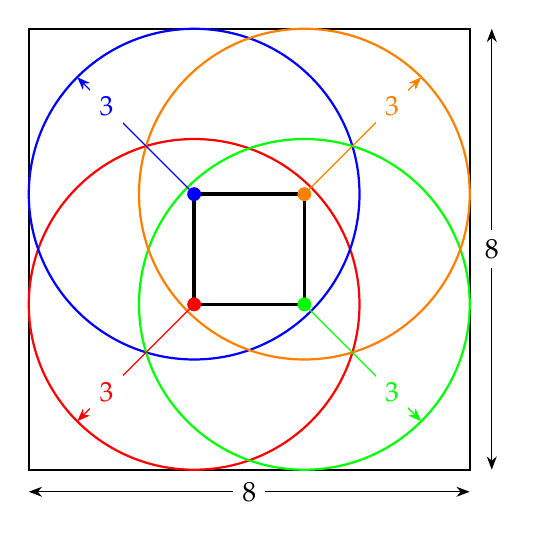
\begin{tikzpicture}[scale=.7]
\coordinate (c1) at (3,3);
\coordinate (c2) at (3,5);
\coordinate (c3) at (5,3);
\coordinate (c4) at (5,5);
\draw[very thick] (c1) -- (c3) -- (c4) -- (c2) -- cycle;
\draw[thick] (0,0) rectangle +(8,8);
\draw[color=red,thick] (c1) circle[radius=3];
\draw[color=blue,thick] (c2) circle[radius=3];
\draw[color=green,thick] (c3) circle[radius=3];
\draw[color=orange,thick] (c4) circle[radius=3];
\vertexcolor{c1}{red};
\vertexcolor{c2}{blue};
\vertexcolor{c3}{green};
\vertexcolor{c4}{orange};
\draw[<->] (0,-.4) -- node[fill=white] {$8$} (8,-.4);
\draw[<->] (8.4,0) -- node[fill=white] {$8$} (8.4,8);
\draw[->,red] (3,3) -- node[near end,fill=white] {$3$} +(-135:3);
\draw[->,blue] (3,5) -- node[near end,fill=white] {$3$} +(135:3);
\draw[->,green] (5,3) -- node[near end,fill=white] {$3$} +(-45:3);
\draw[->,orange] (5,5) -- node[near end,fill=white] {$3$} +(45:3);
\end{tikzpicture}
\caption{Coins contained in the square}\label{f.coins1}
\end{subfigure}
\hspace{3em}
\begin{subfigure}[b]{.43\textwidth}
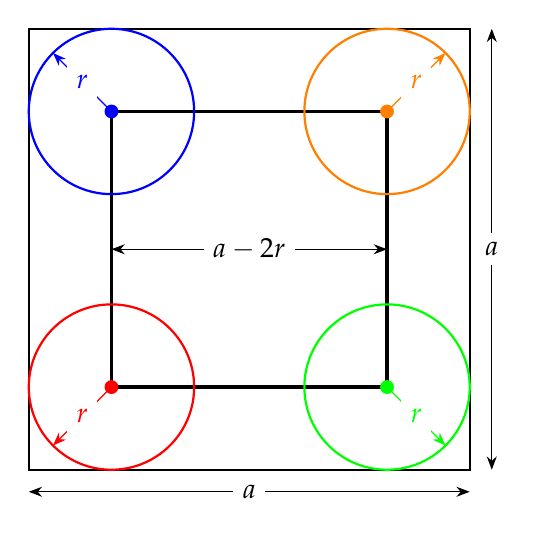
\begin{tikzpicture}[scale=.7]
\coordinate (c1) at (1.5,1.5);
\coordinate (c2) at (1.5,6.5);
\coordinate (c3) at (6.5,1.5);
\coordinate (c4) at (6.5,6.5);
\draw[very thick] (c1) -- (c3) -- (c4) -- (c2) -- cycle;
\draw[thick] (0,0) rectangle +(8,8);
\draw[color=red,thick] (c1) circle[radius=1.5];
\draw[color=blue,thick] (c2) circle[radius=1.5];
\draw[color=green,thick] (c3) circle[radius=1.5];
\draw[color=orange,thick] (c4) circle[radius=1.5];
\vertexcolor{c1}{red};
\vertexcolor{c2}{blue};
\vertexcolor{c3}{green};
\vertexcolor{c4}{orange};
\draw[<->] (0,-.4) -- node[fill=white] {$a$} (8,-.4);
\draw[<->] (8.4,0) -- node[fill=white] {$a$} (8.4,8);
\draw[->,red] (1.5,1.5) -- node[fill=white] {$r$} +(-135:1.5);
\draw[->,blue] (1.5,6.5) -- node[fill=white] {$r$} +(135:1.5);
\draw[->,green] (6.5,1.5) -- node[fill=white] {$r$} +(-45:1.5);
\draw[->,orange] (6.5,6.5) -- node[fill=white] {$r$} +(45:1.5);
\draw[<->] (1.5,4) -- node[fill=white] {$a-2r$} (6.5,4);
\end{tikzpicture}
\caption{Coins in a large square}\label{f.coins2}
\end{subfigure}
\end{center}
\end{figure}

\ans{2}
\[
E(\textsf{winnings per throw})=5\cdot\frac{1}{16}\,+\,(-1)\cdot\frac{15}{16}=-\frac{10}{16}=-0.625\,.
\]

\ans{3} \ref{f.coins2} shows four circles inscribed in the corners of the square. The side of the inner square is $a-2r$ so:
\[
P(\textsf{coin lands within the square})=\frac{(a-2r)^2}{a^2}\,.
\]
\textbf{Simulation}
\begin{verbatim}
For side = 8, radius = 1:
Probability of landing within the square = 0.5625
Proportion landing within the square     = 0.5704
For side = 8, radius = 2:
Probability of landing within the square = 0.2500
Proportion landing within the square     = 0.2481
For side = 8, radius = 3:
Probability of landing within the square = 0.0625
Proportion landing within the square     = 0.0639
For side = 8, radius = 4:
Probability of landing within the square = 0.0000
Proportion landing within the square     = 0.0000
\end{verbatim}

%%%%%%%%%%%%%%%%%%%%%%%%%%%%%%%%%%%%%%%%%%%%%%%%%%%%%%%%%%%%%

\begin{prob}{Chuck-a-luck}
Choose number $n$ between $1$ and $6$ and throw three dice. If $n$ does not appear on any of the dice you lose $1$; if $n$ appears on one die you win $1$; if $n$ appears on two dice you win $2$; if $n$ appears on three dice you win $3$. What is the expectation of your winnings?
\end{prob}

\newpage

\solution{}

Let $P(k)$ be the probability that $n$ appears on $k$ dice. Then:
\[
E(\textsf{winnings per throw})=-1 P(0) + 1 P(1) + 2 P(2) + 3 P(3)\,.
\]
The throws of the three dice are independent so:
\begin{eqn}
E(\textsf{winnings per throw}) &=& 
-1 \dischoose{3}{0}\left(\frac{1}{6}\right)^0\left(\frac{5}{6}\right)^3
+1\dischoose{3}{1}\left(\frac{1}{6}\right)^1\left(\frac{5}{6}\right)^2+\\
&&\;\;\; 2{3\choose 2}\left(\frac{1}{6}\right)^2\left(\frac{5}{6}\right)^1+
3\dischoose{3}{3}\left(\frac{1}{6}\right)^3\left(\frac{5}{6}\right)^0\\
&=& \frac{1}{216}(-125+75+30+3)\approx -0.0787\,.
\end{eqn}%

\textbf{Simulation}
\begin{verbatim}
Expectation of winnings = -0.0787
Average winnings        = -0.0724
\end{verbatim}

%%%%%%%%%%%%%%%%%%%%%%%%%%%%%%%%%%%%%%%%%%%%%%%%%%%%%%%%%%%%%

\begin{prob}{Curing the compulsive gambler}

\label{p.roulette}Roulette is a game played with a wheel having $38$ numbered pockets: $18$ red, $18$ black and $2$ green.\footnote{There are two green pockets in American roulette and one green pocket in European roulette.} The wheel is spun, a ball is thrown onto the wheel and you wait until the ball lands in one of the pockets. The ball lands in a random pocket with uniform distribution. You bet $1$ that the ball will land in a specific numbered (red or black) pocket.\footnote{This is the only type of bet used in the problems in this book.} If the ball lands in that pocket you receive $36$. Your net winnings are actually $35$ because the the $36$ includes the $1$ bet which is returned.

\que{1} What is the expectation your winnings if you play $36$ round of roulette?

\que{2} Your friend offers to bet you $20$ that after $36$ rounds you will have \emph{lost} money. What is the expectation of your winnings, taking into account the money won or lost both from the game and the bet with your friend?
\end{prob}

\solution{}

\ans{1} The probability of winning a single round is $1/38$ so:
\begin{eqn}
E(\textsf{winnings in one round})&=&35\cdot \frac{1}{38} + (-1)\cdot\frac{37}{38} = -\frac{2}{38} \approx -0.0526\\
E(\textsf{winnings in}\;36\;\textsf{rounds})&=&36\cdot -0.05266=-1.8947\,.
\end{eqn}%

\ans{2}
Consider the four outcomes of playing roulette for $36$ rounds:
\begin{itemize}
\item If you lose all the rounds you lose $36$.
\item If you win one round you win $35$ and you lose $35$ on the other rounds no money is won or lost.
\item If you win two rounds you win $70$ and you lose $34$ on the other rounds for a net win of $36$.
\item In general if you win $k$ rounds for $2<k\leq 36$ your net win is $35k - (36-k)>0$.
\end{itemize}
Therefore, you lose the bet only if you lose all rounds:
\begin{eqn}
P(\textrm{losing\ } 36 \textrm{\ rounds})&=&\left(\frac{37}{38}\right)^{36}\approx 0.3829\\
E(\textsf{total winnings})&=&\overbrace{-1.8947}^{\textsf{\small E of all rounds}}+\;\;
\overbrace{-20\cdot 0.3829}^{\textsf{\small lose bet}} \;+\; \overbrace{20\cdot (1-0.3829))}^{\textsf{\small win bet}} \approx 2.7904\,.
\end{eqn}%
Clearly you should take the bet!

\textbf{Simulation}
\begin{verbatim}
Expectation of winning a round = -0.0526
Average winnings for a round   = -0.0593
\end{verbatim}
The simulation showed a large variance which was reduced by running one million trials.

%%%%%%%%%%%%%%%%%%%%%%%%%%%%%%%%%%%%%%%%%%%%%%%%%%%%%%%%%%%%%

\begin{prob}{Perfect bridge hand}
Randomly select $13$ cards from a deck. What is the probability that they will all be of the same suit?
\end{prob}

\solution{1}

There are $\dischoose{52}{13}$ ways of selecting $13$ cards from a deck of $52$ cards. Only four of them consist of $13$ cards from the same suit:
\[
P(\textsf{selecting}\;13\;\textsf{of same suit})=\frac{4}{\dischoose{52}{13}}=\frac{4\cdot 13!\cdot 39!}{52!}\approx 6.2991\times 10^{-12}\,.
\]

\solution{2}

There are $52$ ways of selecting the first card, then $12$ ways of selecting the second card of the same suit from the remaining $51$ cards, $11$ ways of selecting a third card, and so on:
\[
P(\textsf{selecting}\;13\;\textsf{cards of the same suit})=\frac{52}{52}\cdot \frac{12}{51}\cdot \frac{11}{50} \cdots  \frac{1}{40}= \frac{12!}{51!/39!}\approx 6.2991\times 10^{-12}\,.
\]

\newpage

\textbf{Simulation}

There is no point in running a simulation with $52$ cards because the result would almost certainly be zero. A simulation was run with a deck of $16$ cards and $4$ suits.

\begin{verbatim}
Probability of perfect hand = 0.0022
Proportion perfect hand     = 0.0020
\end{verbatim}

%%%%%%%%%%%%%%%%%%%%%%%%%%%%%%%%%%%%%%%%%%%%%%%%%%%%%%%%%%%%%

\begin{prob}{Craps\annotate{D}}
Craps is a played with a pair of dice. On the first throw you win if the sum of the numbers is $7$ or $11$ and you lose if the sum is $2$, $3$ or $12$. If the sum on the first throw is $n=4,5,6,8,9,10$ (called a \emph{point}), continue to throw the dice until the sum is the point $n$ (a win) or $7$ (a loss).

\que{1} What are the probabilities of the following events on the first throw: winning, losing, neither winning nor losing?

\que{2} What is the probability of a win?
\end{prob}

\solution{1}

\ans{1} The outcome of throwing a die is uniformly distributed and the outcomes of throwing a pair of dice are independent, so the probability of any outcome is $1/36$. The number of ways of obtaining each of the events, the sum of a pair of dice, is:
\[
\begin{array}{l|rrrrrrrrrrr}
\textrm{Sum} & 2 & 3 & 4 & 5 & 6 & 7 & 8 & 9 & 10 & 11 & 12\\\hline
\textrm{Pairs} & 1 & 2 & 3 & 4 & 5 & 6 & 5 & 4 & 3 & 2 & 1
\end{array}
\]
On the first throw there are $8$ ways of throwing $7$ or $11$ so the probability of winning is $8/36$ and there are $4$ ways of throwing $2,3,12$ so the probability losing is $4/36$. The probability of neither winning nor losing on the first throw is:
\[
1 - \frac{8}{36} - \frac{4}{36} = \frac{24}{36}\,.
\]

%%%%%%%%%%%%%%%%%%%%%%%%%%%%%%%%%%%%

\ans{2}
Consider two cases:
\begin{itemize}
\item The point is $4$. The probability of winning on the second throw (a $4$) is $3/36$ and the probability of losing (a $7$) is $6/36$. The probability of neither winning nor losing is $1-(3/36)-(6/36)=27/36$.
\item The point is $8$. The probability of winning on the second throw (an $8$) is $5/36$ and the probability of losing (a $7$) is $6/36$. The probability of neither winning nor losing is $1-(5/36)-(6/36)=25/36$.
\end{itemize}
We see that the probability of winning must be computed separately for each of the points $4,5,6,8,9,10$, so we develop a general formula for the probability.

Let $P_n$ be the probability of winning by throwing the point $n$ on a throw and let $Q_n$ the probability of neither winning nor losing on a throw if the point is $n$. $W_n$, the probability of winning by \emph{eventually} throwing the point $n$ after the first throw, is computed by adding:
\begin{itemize}
\item The probability of throwing the point on the second throw.
\item The probability of neither winning nor losing on the second throw and throwing the point on the third throw.
\item The probability of neither winning nor losing on the second and third throws and throwing the point on the fourth throw,
\end{itemize}
and so on:
\begin{eqn}
W_n&=&P_n + Q_n P_n + Q_n^2 P_n+ Q_n^3 P_n  + \cdots\\
&=&P_n\left(1+Q_n^1 + Q_n^2+ Q_n^3  + \cdots\right)\\
&=&P_n\left(\frac{1}{1-Q_n}\right)\,.
\end{eqn}%
You lose on any throw after the first if you throw a $7$ with probability $6/36$ so:
\begin{eqn}
Q_n &=& (1-P_n)-(6/36)\\
W_n&=&\frac{P_n}{P_n+(6/36)}\,.
\end{eqn}%
$W_n$ for the six points are:
\[
\renewcommand{\arraystretch}{2}
\begin{array}{lcccccc}
n   & 4 & 5 & 6 & 8 & 9 & 10 \\\hline
P_n & \disfrac{3}{36} & \disfrac{4}{36} & \disfrac{5}{36} & \disfrac{5}{36} & \disfrac{4}{36} & \disfrac{3}{36} \\
%1-Q_n & \disfrac{9}{36} & \disfrac{10}{36} & \disfrac{11}{36} & \disfrac{11}{36} & \disfrac{10}{36} & \disfrac{9}{36} \\
W_n & \disfrac{3}{9} & \disfrac{4}{10} & \disfrac{5}{11} & \disfrac{5}{11} & \disfrac{4}{10} & \disfrac{3}{9}
\end{array}
\]
$W$, the probability of winning, can be computed by adding the probability of winning on the first throw to the sum of the probabilities for winning by throwing a point each multiplied by the probability of throwing \emph{that point} on the first throw:
\begin{equation}\label{eq.9-a}
W=\frac{8}{36}+\sum_{n\in\{4,5,6,8,9,10\}} P_nW_n \approx 0.4929\,.
\end{equation}
The casino's probability of winning a game of craps is
only $0.5-0.4929\approx 0.5\%$, but the law of large numbers ensures that they will eventually win and you will eventually lose!

%%%%%%%%%%%%%%%%%%%%%%%%%%%%%%%%%%%%

\newpage

\solution{2}

\ans{2} Consider the following sequences of throws where the point is $4$:
\[
\begin{array}{rrrrrrrrrrr}
4 & 8 & 9 & 9 & 9 & 8 & 8 & 8 & 9 & 8 & 4\\
4 & 8 & 9 & 9 & 9 & 8 & 8 & 8 & 9 & 8 & 7\\
4 & 9 & 9 & 9 & 8 & 8 & 4
\end{array}
\]
The games only terminates if a $4$ is thrown (win) or a $7$ is thrown (loss), so an appearance of an $8$ or a $9$ doesn't affect the result. Therefore, once a point has been thrown, the probability of winning is the conditional probability that a $4$ is thrown given that a $4$ or  a $7$ is thrown. Let $f$ be the event that a $4$ is thrown and $s$ be the event that a $7$ is thrown. Then:
\[
P(f|f\cup s) = \disfrac{P(f)\cap P(f\cup s)}{P(f\cup s)}=\disfrac{P(f)}{P(f\cup s)}=\disfrac{3/36}{(3+6)/36}=\disfrac{3}{9}\,,
\]
which is exactly the result $W_4$ in the table above. After computing $W_n$ for all points, Equation~\ref{eq.9-a} can be used to compute $W$.

Conditional probability is implicitly used in the first solution because $W_n$ is a probability that is conditional on the first throw resulting in the point $n$.

\textbf{Simulation}
\begin{verbatim}
Probability of winning = 0.4929
Proportion of wins     = 0.4948
\end{verbatim}

%%%%%%%%%%%%%%%%%%%%%%%%%%%%%%%%%%%%%%%%%%%%%%%%%%%%%%%%%%%%%

\refstepcounter{problem}  % 10. An experiment in personal taste

%%%%%%%%%%%%%%%%%%%%%%%%%%%%%%%%%%%%%%%%%%%%%%%%%%%%%%%%%%%%%

\refstepcounter{problem}  % 11. Silent cooperation

%%%%%%%%%%%%%%%%%%%%%%%%%%%%%%%%%%%%%%%%%%%%%%%%%%%%%%%%%%%%%

\refstepcounter{problem}  % 12. Quo vadis?

%%%%%%%%%%%%%%%%%%%%%%%%%%%%%%%%%%%%%%%%%%%%%%%%%%%%%%%%%%%%%

\begin{prob}{The prisoner's dilemma}

Three prisoners $A,B,C$ are eligible for parole. The parole board will release two of them with equal probability for $\{A,B\}, \{A,C\}, \{B,C\}$, so the probability that $A$ will be released is $2/3$. Prisoner $A$ is told correctly the name of  one of the other prisoners $B$ or $C$ who will be released. If $A$ is told that prisoner $B$ will be released, what is the probability that $A$ too will be released?

\cite{carlton} is devoted to the prisoner's dilemma and to the similar Monty Hall problem.
\end{prob}

\solution{1}

Let $P(A), P(B), P(C)$ be the probabilities that $A,B,C$ are released. $A$ is interested in the conditional probability $P(A|B)$ of his being released if $B$ will be released:
\[
P(A|B) = \frac{P(A\cap B)}{P(B)} = \frac{1/3}{2/3}=\frac{1}{2}\,.
\]
But that is \emph{not} the correct conditional probability! Let $R_{AB}$ be the event that $A$ is \emph{told} that $B$ will be released. The probability that must be computed is $P(A|R_{AB})$:
\[
P(A|R_{AB}) = \frac{P(A\cap R_{AB})}{P(R_{AB})}\,.
\]
We assume that the report of $B$'s release is true so:
\[
P(A\cap R_{AB})=P(\{A,B\})=\disfrac{1}{3}\,.
\]
Now:
\[
P(R_{AB})=P(\{A,B\})+P(\{B,C\})=\disfrac{1}{3}+\disfrac{1}{2}\cdot \disfrac{1}{3}=\disfrac{1}{2}\,.
\]
If $\{B,C\}$ are to be released $A$ could be \emph{told} that either $B$ or $C$ is to be released, hence the factor of $1/2$. Therefore:
\[
P(A|R_{AB}) = \frac{P(A\cap R_{AB})}{P(R_{AB})} = \disfrac{1/3}{1/2}=\disfrac{2}{3}\,,
\]
so if $A$ is told that $B$ will be released the probability that $A$ will be released does not change.

\solution{2}

There are four possible events:
\begin{description}
\item[$e_1$:] $A$ is told that $B$ will be released and $\{A,B\}$ are released. 
\item[$e_2$:] $A$ is told that $C$ will be released and $\{A,C\}$ are released. 
\item[$e_3$:] $A$ is told that $B$ will be released and $\{B,C\}$ are released. 
\item[$e_4$:] $A$ is told that $C$ will be released and $\{B,C\}$ are released. 
\end{description}
Each pair of prisoners has equal probability of being released so:
\[
P(e_1)=P(e_2)=P(e_3\cup e_4)=\frac{1}{3}\,.
\]
If $\{B,C\}$ are to be released, $A$ is told correctly the name of either $B$ or $C$ who will be released and the probability of being told either of the names is equal, so $P(e_3)=P(e_4)=1/6$. Therefore the probability that $A$ will be released given the event $R_{AB}=e_1\cup e_3$ that $A$ is told that $B$ will be released is:
\[
P(A|R_{AB}) = \frac{P(e_1\cap(e_1\cup e_3))}{P(e_1\cup e_3)}=\frac{P(e_1)}{P(e_1\cup e_3)}=\frac{1/3}{(1/3)+(1/6)}=\frac{2}{3}\,.
\]

\solution{3}

A riddle attributed to Abraham Lincoln asks: ``If you call the tail of a dog a leg, how many legs does the dog have?'' The answer is that calling a tail a leg doesn't make it a leg, so the dog still has four legs. Clearly, whether $A$ knows $B$'s future or not doesn't change his chances of being released.

\newpage

\textbf{Simulation}

There is no simulation: the problem asks if the probability changes as the result of some knowledge but we have shown that it does not change.

%%%%%%%%%%%%%%%%%%%%%%%%%%%%%%%%%%%%%%%%%%%%%%%%%%%%%%%%%%%%%

\begin{prob}{Collecting coupons}
Given a unbounded sequence of boxes each of which contains five coupons numbered $1$ to $5$, you randomly draw one coupon sequentially from each box.

\que{1} What is the expectation of the number of coupons drawn until you have all five of the numbers?

\que{2} Develop a formula for the expectation for $n$ numbers.

\textbf{Hint:} Use the solution to Problem~4 on page~\pageref{p.four} and the approximation for $H_n$, the sum of harmonic numbers (page~\pageref{p.harmonic}).
\end{prob}

\solution{}

\ans{1} What is the expectation of the number of draws until you get a  number that is \emph{different from} all the previous ones? By  Problem~4 this is $1/p$ where $p$ is the probability of drawing a different number. For the first draw the probability is $1$ so the expectation is $1=5/5$, for the second draw the probability is $4/5$ so expectation is $5/4$, and so on. Therefore:
\[
E(\textsf{all five numbers}) = \frac{5}{5}+\frac{5}{4} + \frac{5}{3} + \frac{5}{2} + \frac{5}{1} = \frac{}{} =\frac{1370}{120}\approx 11.4167\,.
\]
\ans{2} Use the same method and the approximation for $H_n$:
\[
E(\textsf{all}\;n \;\textsf{numbers}) = n\left(\frac{1}{n}+\frac{1}{n-1} + \cdots \frac{1}{2} + \frac{1}{1}\right) =nH_n\approx n\left(\ln n + \frac{1}{2n} + 0.5772\right)\,. 
\]
For $n=5$ this gives:
\[
E(\textsf{all five numbers}) =5H_5\approx 5\left(\ln 5 + \frac{1}{10} + 0.5772\right) \approx 11.4332\,.
\]

\textbf{Simulation}
\begin{verbatim}
For  5 coupons:
Expectation of draws = 11.4332
Average draws        = 11.3339
For 10 coupons:
Expectation of draws = 29.2979
Average draws        = 29.3001
For 20 coupons:
Expectation of draws = 71.9586
Average draws        = 71.6250
\end{verbatim}

%%%%%%%%%%%%%%%%%%%%%%%%%%%%%%%%%%%%%%%%%%%%%%%%%%%%%%%%%%%%%

\begin{prob}{The theater row}
Arrange $8$ even numbers and $7$ odd numbers randomly in a row, for example:
\[
10\quad 12\quad 3\quad 2\quad 9\quad 6 \quad 1\quad 13\quad 7\quad 10\quad 3\quad 8\quad 8\quad 5\quad 20\,,
\]
which we can write as follows since the specific numbers are not important:
\[
E\quad E\quad O\quad E\quad O\quad E \quad O\quad O\quad O\quad E\quad O\quad E\quad E\quad O\quad E\,.
\]
What is the expectation of the number of even-odd or odd-even adjacent pairs?

In the example there are $10$ $EO$ or $OE$ adjacent pairs.

\textbf{Hint:} What is the probability that a pair of adjacent number are different?
\end{prob}

\solution{}

The following table shows the $10$ possible arrangements of $3$ even and $2$ odd numbers. The total number of different adjacent pairs is $24$ and the average is $24/10=2.4$.
\[
\begin{array}{l|r@{\hspace{2em}}|@{\hspace{2pt}}|@{\hspace{2em}}l|r}
\textsf{Arrangement}&\textsf{Pairs}&\textsf{Arrangement}&\textsf{Pairs}\\\hline
EEEOO & 1&
EEOEO & 3\\
EEOOE & 2&
EOEOE & 4\\
EOEEO & 3&
EOOEE & 2\\
OEEOE & 3&
OEEEO & 2\\
OEOEE & 3&
OOEEE & 1\\
\end{array}
\]
Returning to the example with $15$ numbers, let $P_d$ be the probability that a given pair in an arrangement is $EO$ or $OE$:
\[
P_d =P(EO) + P(OE) = \frac{8}{15}\cdot \frac{7}{14} + \frac{7}{15}\cdot \frac{8}{14} = 2\cdot \frac{8}{15}\cdot \frac{7}{14} = \frac{8}{15}\,.
\]
Let $E_d$ be the expectation of the number of pairs in an arrangement that are $EO$ or $OE$. Since an $EO$ or $OE$ pair contributes $1$ to the count of different pairs and an $EE$ or an $OO$ pair contributes $0$:
\[
E_d =
\sum_{\textsf{\footnotesize all pairs}} (1\cdot P_d + 0\cdot (1-P_d))= 14\cdot \frac{8}{15} \approx 7.4667\,.
\]

Check for $10$ numbers:
\begin{eqn}
P_d &=& P(EO) + P(OE) = \frac{3}{5}\cdot \frac{2}{4} + \frac{2}{5}\cdot \frac{3}{4} = \frac{3}{5}\\
E_d &=& 4\cdot \frac{3}{5}=\frac{12}{5}=2.4\,.
\end{eqn}%

\newpage

\textbf{Simulation}
\begin{verbatim}
For  5 places:
Expectation of different pairs = 2.4000
Average different pairs        = 2.3855
For 15 places:
Expectation of different pairs = 7.4667
Average different pairs        = 7.4566
For 27 places:
Expectation of different pairs = 13.4815
Average different pairs        = 13.4835
For 49 places:
Expectation of different pairs = 24.4898
Average different pairs        = 24.4725
\end{verbatim}

%%%%%%%%%%%%%%%%%%%%%%%%%%%%%%%%%%%%%%%%%%%%%%%%%%%%%%%%%%%%%

\begin{prob}{Will the second-best be runner-up?}
Eight players $\{a_1,\ldots,a_8\}$ are randomly assigned to play eight games $\{g_1,\ldots,g_8\}$ in a tournament such that player $a_{k_i}$ plays his first game in place $g_i$ (Figure~\ref{f.tournament}). The players are ranked from the best $a_1$ to the worst $a_8$ and the better player will \emph{always} defeat his opponent.  Clearly $a_1$ will win the tournament.

\que{1} What is the probability that $a_2$ will be the runner-up by playing $a_1$ in the final round and losing?

\que{2} If there are $2^n$ players what is the probability that $a_2$ will be the runner-up by playing $a_1$ in the final round and losing?
\begin{figure}[tb]
\begin{center}
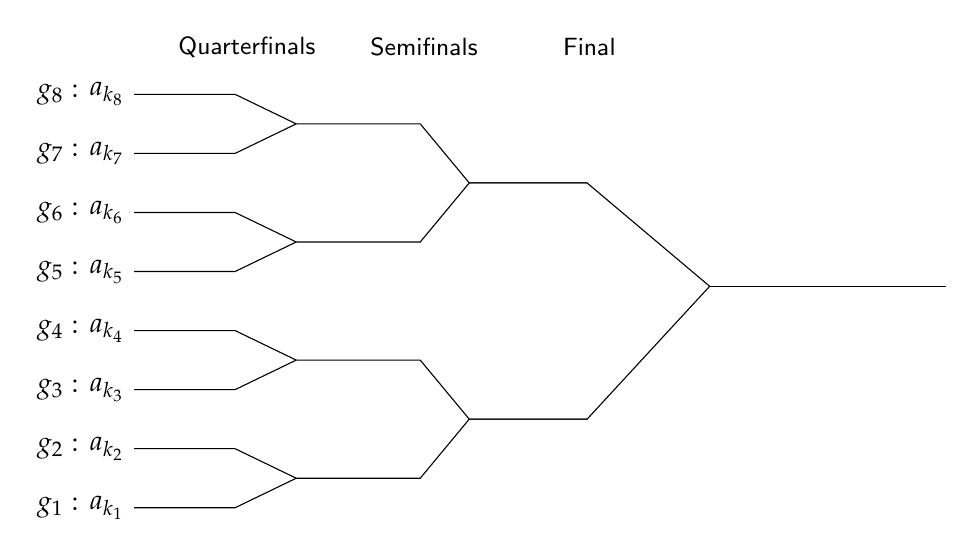
\begin{tikzpicture}[scale=.75]
\foreach \n in {1,2,3,4,5,6,7,8}
  \node (\n) at (0,\n*10mm) {$g_{\n}:$};
\foreach \n in {1,2,3,4}
  \node[inner sep=-4pt] (r\n) at (40mm,-5mm+\n*20mm) {};
\foreach \n/\r in {1/1,2/1,3/2,4/2,5/3,6/3,7/4,8/4}
  \draw (\n) --
     node[very near start,fill=white] {$a_{k_{\n}}$} +(30mm,0)
     -- ($(r\r)+(1pt,0)$);
\foreach \n/\v in {1/25mm,2/65mm}
  \node[inner sep=-5pt] (rr\n) at (70mm,\v) {};
\foreach \n/\r in {1/1,2/1,3/2,4/2}
  \draw ($(r\n)+(1pt,0)$) -- ++(21mm,0) -- 
  ($(rr\r)+(-1pt,0)$) -- ++(20mm,0);
\node[inner sep=-5pt] (rrr) at ($(rr1)+(40mm,22.5mm)$) {};
\foreach \n/\r in {1,2}
 \draw ($(rr\n)+(19.6mm,0)$) -- ($(rrr)+(1pt,0)$); 
\draw ($(rrr)+(1pt,0)$) -- +(40mm,0);
\node at (32mm,88mm) {\textsf{\small Quarterfinals}};
\node at (62mm,88mm) {\textsf{\small Semifinals}};
\node at (90mm,88mm) {\textsf{\small Final}};
\end{tikzpicture}
\end{center}
\caption{A tournament schedule}\label{f.tournament}
\end{figure}
\end{prob}

\newpage

\solution{}

\ans{1}
If $a_1$ is assigned to one of the games $\{g_1,g_2,g_3,g_4\}$ none of the other players assigned to these games will reach the final, so $a_2$ must be assigned to one of $\{g_5,g_6,g_7,g_8\}$. The temptation is to conclude that the probability of $a_2$ being the runner-up is $1/2$ since $a_2$ must be assigned to one of the four games $\{g_1,g_2,g_3,g_4\}$. However, whatever game $a_1$ is  assigned to, $a_2$ will be the runner up only if he is assigned to one of the four \emph{remaining} seven games so the probability is $4/7$.

\ans{2} Similarly, of the $2^n-1$ games that $a_1$ is not assigned to, $a_2$ must be assigned to one of the $2^{n-1}$ games not in the same half as $a_1$. Therefore:
\[
P(a_1,a_2\;\textsf{playing each other in the final})=\frac{2^{n-1}}{2^n-1}\,.
\]

\textbf{Simulation}
\begin{verbatim}
For   8 players:
Probability a2 is runner-up                = 0.5714
Proportion of games where a2 is runner-up  = 0.5707
For  32 players:
Probability a2 is runner-up                = 0.5161
Proportion of games where a2 is runner-up  = 0.5184
For 128 players:
Probability a2 is runner-up                = 0.5039
Proportion of games where a2 is runner-up  = 0.5060
\end{verbatim}

%%%%%%%%%%%%%%%%%%%%%%%%%%%%%%%%%%%%%%%%%%%%%%%%%%%%%%%%%%%%%

\begin{prob}{Twin knights\annotate{D}}

Eight players $\{a_1,\ldots,a_8\}$ are randomly assigned to play games $\{g_1,\ldots,g_8\}$ in a tournament (Figure~\ref{f.tournament}). Let $P(i,j)$ be the probability that $a_i$ wins against $a_j$. For all $i,j$, $P(i,j)=P(j,i)=1/2$.

\que{1} What is the probability that $a_1,a_2$ play each other?

\que{2} If there are $2^n$ players what is the probability that $a_1,a_2$ play each other?
\end{prob}

\solution{}

\ans{1} Without loss of generality assign $a_1$ to $g_1$. Consider the different possibilities that $a_1,a_2$ play each other. With probability $1/7$, $a_2$ is assigned to $g_2$. With probability $2/7$, $a_2$ is assigned to $g_3$ or $g_4$, but $a_2$ doesn't play $a_1$ unless \emph{both} of them win their first game, so we need to multiply the probability of this assignment by $1/4$. With probability $4/7$, $a_2$ is assigned to $g_5,g_6,g_7,g_8$, but $a_2$ doesn't play $a_1$ unless \emph{both} of them win their first two  games, so we need to multiply the probability of this assignment by $1/16$. Therefore:
\[
P(a_1, a_2\;\textsf{play each other})=\frac{1}{7} + \frac{1}{4}\cdot \frac{2}{7} + \frac{1}{16}\cdot \frac{4}{7} =\frac{1}{4}\,.
\]

\ans{2}
Let $P_n$ be the probability that in a tournament with $2^n$ players $a_1$ and $a_2$ play each other. We have shown that $P_3=1/4$. What about $P_4$? Using the same approach:
\begin{eqn}
P_4 &=& \frac{1}{15} + \frac{1}{4}\cdot \frac{2}{15}  + \frac{1}{16}\cdot \frac{4}{15}  + \frac{1}{64}\cdot \frac{8}{15} \\
&=&\frac{1}{15}\left(1+\frac{1}{2}+\frac{1}{4}+\frac{1}{8}\right)=\frac{1}{8}\,.
\end{eqn}%
It is reasonable to conjecture that $P_n=1/2^{n-1}$.

\textbf{Proof 1:} Using the same approach and the formula for the sum of a geometric series:
\begin{eqn}
P_n&=&\frac{1}{2^n-1}\sum_{i=0}^{n-1}2^i\cdot \left(\frac{1}{2}\right)^{2i}\\
&=&\frac{1}{2^n-1}\sum_{i=0}^{n-1}2^{-i}\\
&=&\frac{1}{2^n-1}
  \left(
    \frac{1-(1/2)^{(n-1)+1}}
         {1-(1/2)}
  \right)=\frac{1}{2^{n-1}}\,.
\end{eqn}%

\textbf{Proof 2:} By induction. The base case is $P_3=1/4=1/2^{3-1}$.

There are two inductive steps:

\textit{Case 1:} $a_1$ and $a_2$ are assigned to different halves of the tournament:
\[
P(a_1,a_2\;\textsf{assigned to different halves})=\frac{2^{n-1}}{2^n-1}\,.
\]
They can only meet in the final game and therefore both must win all of their $n-1$ games:
\begin{equation}\label{eq.17a}
P(a_1,a_2\;\textsf{meet if assigned to different halves})=\frac{2^{n-1}}{2^n-1} \left(\frac{1}{2}\right)^{n-1} \left(\frac{1}{2}\right)^{n-1}=\frac{2^{-(n-1)}}{2^n-1}\,.
\end{equation}
\textit{Case 2:} $a_1$ and $a_2$ are assigned to the same half of the tournament:
\[
P(a_1,a_2\;\textsf{assigned to the same half})=\frac{2^{n-1}-1}{2^n-1}\,.
\]
Since both players are in the same half the problem has been reduced to determining $P_{n-1}$. By the inductive hypothesis:
\begin{equation}\label{eq.17b}
P(a_1,a_2\;\textsf{meet if assigned to the same half})=\frac{2^{n-1}-1}{2^n-1}\cdot \frac{1}{2^{n-2}}=\frac{2^{1}-2^{-(n-2)}}{2^n-1}\,.
\end{equation}
Combining Equations~\ref{eq.17a}, \ref{eq.17b} gives:
\[
\renewcommand*{\arraystretch}{2.2}
\begin{array}{rcl}
P_n&=&\disfrac{2^{-(n-1)}}{2^n-1}+\disfrac{2^{1}-2^{-(n-2)}}{2^n-1}\\
&=&\disfrac{2^{n-1}}
        {2^{n-1}}\cdot 
   \disfrac{2^{-(n-1)}+2^{1}-2^{-(n-2)}}
        {2^n-1}\\
&=&\disfrac{1}
        {2^{n-1}}\cdot 
   \disfrac{2^0+2^n-2^1}
        {2^n-1}=\disfrac{1}{2^{n-1}}\,.
\end{array}
\]

\textbf{Simulation}
\begin{verbatim}
For   8 players:
Probability that a1, a2 meet = 0.2500
Proportion a1, a2 meet       = 0.2475
For  32 players:
Probability that a1, a2 meet = 0.0625
Proportion a1, a2 meet       = 0.0644
For 128 players:
Probability that a1, a2 meet = 0.0156
Proportion a1, a2 meet       = 0.0137
\end{verbatim}

%%%%%%%%%%%%%%%%%%%%%%%%%%%%%%%%%%%%%%%%%%%%%%%%%%%%%%%%%%%%%

\begin{prob}{An even split at coin tossing}
\que{1} Toss a fair coin $20$ times. What is the probability of obtaining $10$ heads?

\que{2} Toss a fair coin $40$ times. What is the probability of obtaining $20$ heads?
\end{prob}

\solution{}

\ans{1} Since the coin is fair the probability of obtaining $10$ heads in $20$ tosses is given by the binomial distribution:
\[
P(10\;\textsf{heads in}\; 20\; \textsf{tosses})={20 \choose 10} \left(\frac{1}{2}\right)^{10}\left(\frac{1}{2}\right)^{10} \approx 0.1762\,.
\]

\ans{2} You might expect the probability to be the same before but:
\[
P(20\;\textsf{heads in}\; 40\; \textsf{tosses})={40 \choose 20} \left(\frac{1}{2}\right)^{20}\left(\frac{1}{2}\right)^{20}\approx 0.1254\,.
\]
By the law of large numbers the numbers of heads and tails will be ``roughly'' equal \cite[Section~8.4]{ross}, but they are unlikely to be exactly the same, and this event becomes less likely as the number of tosses increases.

\newpage

\textbf{Simulation}
\begin{verbatim}
Probability of 10 heads for  20 tosses = 0.1762
Proportion  of 10 heads for  20 tosses = 0.1790
Probability of 20 heads for  40 tosses = 0.1254
Proportion  of 20 heads for  40 tosses = 0.1212
Probability of 50 heads for 100 tosses = 0.0796
Proportion  of 50 heads for 100 tosses = 0.0785
\end{verbatim}

%%%%%%%%%%%%%%%%%%%%%%%%%%%%%%%%%%%%%%%%%%%%%%%%%%%%%%%%%%%%%

\begin{prob}{Isaac Newton helps Samuel Pepys}
\que{1} What is the probability of obtaining \emph{at least one} $6$ when $6$ dice are thrown?

\que{2} What is the probability of obtaining \emph{at least two} $6$'s when $12$ dice are thrown?

\que{3} Develop a formula for the probability of obtaining at least $n$ $6$'s when $6n$ dice are thrown.
\end{prob}

\solution{}

\ans{1} The probability is the complement of the probability of obtaining zero $6$'s in $6$ throws:
\[
P(\textsf{at least one}\; 6)=1-\left(\frac{5}{6}\right)^6\approx 0.6651\,.
\]

\ans{2} The probability is the complement of the probability of obtaining zero or one $6$'s in $12$ throws:
\[
P(\textsf{at least two}\;6\textsf{s})=1-\left(\frac{5}{6}\right)^{12}-{12\choose 1}\left(\frac{1}{6}\right)^{1}\left(\frac{5}{6}\right)^{11}\approx 0.6187\,.
\]
This event is less probable than the previous one.

\ans{3} The probability is the complement of the probability of obtaining less than $n$ $6$'s in $6n$ throws:
\begin{eqn}
P(\textsf{at least}\;n\;6\textsf{s})&=&
  1-{6n \choose 0}\left(\frac{1}{6}\right)^0\left(\frac{5}{6}\right)^{6n-0}-
  {6n\choose 1}\left(\frac{1}{6}\right)^{1}\left(\frac{5}{6}\right)^{6n-1}-\cdots\\
&=&1-\sum_{i=0}^{n-1}{6n\choose i}\left(\frac{1}{6}\right)^{i}\left(\frac{5}{6}\right)^{6n-i}\,.
\end{eqn}%

\textbf{Simulation}
\begin{verbatim}
For   6 dice to throw  1 sixes:
Probability = 0.6651
Proportion  = 0.6566
For  12 dice to throw  2 sixes:
Probability = 0.6187
Proportion  = 0.6220
For  18 dice to throw  3 sixes:
Probability = 0.5973
Proportion  = 0.5949
For  96 dice to throw 16 sixes:
Probability = 0.5424
Proportion  = 0.5425
For 360 dice to throw 60 sixes:
Probability = 0.5219
Proportion  = 0.5250
\end{verbatim}

%%%%%%%%%%%%%%%%%%%%%%%%%%%%%%%%%%%%%%%%%%%%%%%%%%%%%%%%%%%%%

\begin{prob}{The three-cornered duel\annotate{D}}
$A,B,C$ fight a sequence of duels. Each of them has a fixed probability of winning a duel regardless of who the opponent is:
\[
P(A)=0.3,\quad P(B)=1, \quad P(C)=0.5\,.
\]
A person who is hit no longer participates in the duels. The shots are fired one at a time sequentially in the order $A,B,C$. If two opponents are still standing the shooter can decide whom to fire at. Assume that each person makes the optimal decision for each duel.

\que{1} What is $A$'s best strategy?

\que{2} Suppose that $A$ fires the first shot into the air. Is this a better strategy?

\textbf{Hint:} Give a formal definition for one strategy is better than another.

\textbf{Hint:} Compute the conditional probabilities of $A$ winning depending on whether $A$ chooses to shoot first at $B$ or $C$.
\end{prob}

\solution{}

Let $I_X$ be the indicator variable for $X$ winning the sequence of duels:
\[
I_X=
\left\{
\begin{array}{ll}
1,\quad X\;\textsf{wins the sequence of duels}\\
0, \quad X\; \textsf{loses the sequence of duels}\,.
\end{array}
\right.
\]
Strategy $s_1$ for $X$ is better strategy $s_2$ if the expectation of $I_X$ is greater for $s_1$ than for $s_2$.

Notation: \duel{X}{H}{Y} denotes that $X$ shoots at $Y$ and hits. \duel{X}{M}{Y} denotes that $X$ shoots at $Y$ and misses.

\ans{1}
Compute the conditional probabilities of $A$ winning.

\textit{Case 1:} $A$ chooses to shoot first at $C$.

If \duel{A}{M}{C} (probability $0.7$) then \duel{B}{H}{C} since $C$ is more dangerous than $A$. $A$ now shoots again at $B$ with probability $0.3$ of hitting, but if $A$ misses then \duel{B}{H}{A} with probability $1$ and $A$ loses.

If \duel{A}{H}{C} (probability $0.3$) then \duel{B}{H}{A} with probability $1$ and $A$ loses.

\vspace*{-3ex}
\[
\renewcommand*{\arraystretch}{2.5}
\begin{array}{l}
E(A \;\textsf{wins}\;|A\;\textsf{chooses to shoot first at}\;C) =\\
%
\qquad\quad \overbrace{1\cdot (0.7\cdot 1 \cdot 0.3)}^%
{\duelmath{A}{M}{C}, \duelmath{B}{H}{C}, \duelmath{A}{H}{B}}\; +
%
\overbrace{0\cdot (0.7\cdot 1\cdot 0.7\cdot 1)}^%
{\duelmath{A}{M}{C},  \duelmath{B}{H}{C}, \duelmath{A}{M}{B}, \duelmath{B}{H}{A}}+
%
\;\;\overbrace{0\cdot (0.3\cdot 1)}^%
{\duelmath{A}{H}{C}, \duelmath{B}{H}{A}}=0.2100\,.
\end{array}
\]
\textit{Case 2:} $A$ chooses to shoot first at $B$.

If \duel{A}{M}{B} (probability $0.7$) then as before \duel{B}{H}{C} and $A$ has one more chance to hit $B$ (probability $0.3$), otherwise \duel{B}{H}{A} with probability $1$ and $A$ loses.

If \duel{A}{H}{B} (probability $0.3$) then $A,C$ alternately shoot at each other until one is hit. The possibilities are:
\[
\begin{array}{ll}
(1)&C\stackrel{H}{\longrightarrow}A\\
(2)&C\stackrel{M}{\longrightarrow}A \stackrel{H}{\longrightarrow}C\\
(3)&C\stackrel{M}{\longrightarrow}A \stackrel{M}{\longrightarrow}C\stackrel{H}{\longrightarrow}A\\
(4)&C\stackrel{M}{\longrightarrow}A \stackrel{M}{\longrightarrow}C\stackrel{M}{\longrightarrow}A\stackrel{H}{\longrightarrow}C\\
(5)&C\stackrel{M}{\longrightarrow}A \stackrel{M}{\longrightarrow}C\stackrel{M}{\longrightarrow}A\stackrel{M}{\longrightarrow}C\stackrel{H}{\longrightarrow}A\\
(6)&C\stackrel{M}{\longrightarrow}A \stackrel{M}{\longrightarrow}C\stackrel{M}{\longrightarrow}A\stackrel{M}{\longrightarrow}C\stackrel{M}{\longrightarrow}A\stackrel{H}{\longrightarrow}C\\
&\cdots
\end{array}
\]
The probability of $A$ wins by eventually hitting $C$ is the sum of the probabilities of the even-numbered scenarios in the list:
\begin{eqn}
P(A\;\textsf{wins} \;| A\; \textsf{hits}\;B )&=&(0.5 \cdot 0.3) + \\
&&(0.5 \cdot 0.7) (0.5 \cdot 0.3) + \\
&&(0.5 \cdot 0.7) (0.5 \cdot 0.7) (0.5 \cdot 0.3)+ \cdots\\
&=&0.15 \sum_{i=0}^{\infty} 0.35^i= \frac{0.15}{1-0.35}=\frac{3}{13}\approx 0.2308\,.
\end{eqn}%
Similarly, the probability of $C$ winning is $\disfrac{0.5}{1-0.35}=\disfrac{10}{13}\approx 0.7692$.

The expectation is:
\vspace*{-1ex}
\[
\renewcommand*{\arraystretch}{1.5}
\begin{array}{l}
E(A \;\textsf{wins}) =E(A \;\textsf{wins}\;|\;A\;\textsf{misses}\;B) + E(A \;\textsf{wins}\;|\;A\;\textsf{hits}\;B)=\\
\qquad\qquad
\overbrace{1\cdot (0.7\cdot 1\cdot 0.3)}%
^{A\stackrel{M}{\longrightarrow}B, B\stackrel{H}{\longrightarrow}C, A\stackrel{H}{\longrightarrow}B}\;+
%
\overbrace{0\cdot (0.7\cdot 1\cdot 0.7\cdot 1)}%
^{A\stackrel{M}{\longrightarrow}B,
B\stackrel{H}{\longrightarrow}C,
A\stackrel{M}{\longrightarrow}B,
B\stackrel{H}{\longrightarrow}A}\; +
%
\overbrace{1\cdot 0.2308}%
^{A\stackrel{H}{\longrightarrow}B,
C\stackrel{H}{\longleftrightarrow*}A,
A\stackrel{H}{\longrightarrow}C}\; +\\
%
\qquad\;\,\overbrace{0\cdot 0.7692}%
^{A\stackrel{H}{\longrightarrow}B,
C\stackrel{H}{\longleftrightarrow*}A,
C\stackrel{H}{\longrightarrow}A}
\approx \; 0.2792\,,
\end{array}
\]
which is higher than the expectation of winning by shooting at $C$ first.

\ans{2} If $A$ shoots into the air not hitting anyone (probability $1$) then $B\stackrel{H}{\longrightarrow}C$ with probability $1$ and $A$ can try to hit $B$ with probability $0.3$. The expectation is:
\[
E(A \;\textsf{wins}|A\;\textsf{shoots in the air}) = 1\cdot (1\cdot 1 \cdot 0.3) + 0\cdot(1\cdot 1\cdot 0.7)=0.3\,,
\]
which is higher than the expectation for the other two strategies!

\textbf{Simulation}
\begin{verbatim}
For A fires first at C:
Expectation of wins = 0.2100
Average wins        = 0.2138
For A fires first at B:
Expectation of wins = 0.2792
Average wins        = 0.2754
For A fires in the air:
Expectation of wins = 0.3000
Average wins        = 0.3000
\end{verbatim}

%%%%%%%%%%%%%%%%%%%%%%%%%%%%%%%%%%%%%%%%%%%%%%%%%%%%%%%%%%%%%

% !TeX root = mos-en.tex

%%%%%%%%%%%%%%%%%%%%%%%%%%%%%%%%%%%%%%%%%%%%%%%%%%%%%%%%%%%%%

\refstepcounter{problem}  % 11. Silent cooperation

%%%%%%%%%%%%%%%%%%%%%%%%%%%%%%%%%%%%%%%%%%%%%%%%%%%%%%%%%%%%%

\refstepcounter{problem}  % 12. Quo vadis?

%%%%%%%%%%%%%%%%%%%%%%%%%%%%%%%%%%%%%%%%%%%%%%%%%%%%%%%%%%%%%

\begin{prob}{The prisoner's dilemma\annotate{D}}

Three prisoners $A,B,C$ are eligible for parole. The parole board will release two of them with equal probability for $\{A,B\}, \{A,C\}, \{B,C\}$, so the probability that $A$ will be released is $2/3$. Prisoner $A$ is told the name of one of the other prisoners who will be released. If he is told that prisoner $B$ will be released, what is the probability that $A$ too will be released?

For a comprehensive article on the prisoner's dilemma problem and the related Monty Hall problem see \cite{carlton}.
\end{prob}

\solution{1}

Let $P(A), P(B), P(C)$ be the probabilities that $A,B,C$ are released. $A$ is interested in the conditional probability $P(A|B)$ of his being released if $B$ will be released:
\[
P(A|B) = \frac{P(A\cap B)}{P(B)} = \frac{1/3}{2/3}=\frac{1}{2}\,.
\]
But that is \emph{not} the correct conditional probability! Let $R_{AB}$ be the event that $A$ is \emph{told} that $B$ will be released. The probability that must be computed is $P(A|R_{AB})$:
\[
P(A|R_{AB}) = \frac{P(A\cap R_{AB})}{P(R_{AB})}\,.
\]
We assume that the report of $B$'s release is true so:
\[
P(A\cap R_{AB})=P(\{A,B\})=\disfrac{1}{3}\,.
\]
Now:
\[
P(R_{AB})=P(\{A,B\})+P(\{B,C\})=\disfrac{1}{3}+\disfrac{1}{2}\cdot \disfrac{1}{3}=\disfrac{1}{2}\,.
\]
If $\{B,C\}$ are to be released, $A$ could be told that either $B$ or $C$ is to be released, hence the factor of $1/2$. Therefore:
\[
P(A|R_{AB}) = \frac{P(A\cap R_{AB})}{P(R_{AB})} = \disfrac{1/3}{1/2}=\disfrac{2}{3}\,,
\]
so if $A$ is told that $B$ will be released the probability that he will be released does not change.

\solution{2}

There are four possible events:
\begin{description}
\item[$e_1$:] $A$ is told that $B$ will be released and $\{A,B\}$ are released. 
\item[$e_2$:] $A$ is told that $C$ will be released and $\{A,C\}$ are released. 
\item[$e_3$:] $A$ is told that $B$ will be released and $\{B,C\}$ are released. 
\item[$e_4$:] $A$ is told that $C$ will be released and $\{B,C\}$ are released. 
\end{description}
Each pair of prisoners has equal probability of being released so:
\[
P(e_1)=P(e_2)=P(e_3\cup e_4)=\frac{1}{3}\,.
\]
We assume that if $\{B,C\}$ are to be released, $A$ is told $B$ or $C$ with equal probability, so $P(e_3)=P(e_4)=1/6$. Therefore the probability that $A$ will be released given the event $R_{AB}=e_1\cup e_3$ that he is told that $B$ will be released is:
\[
P(A|R_{AB}) = \frac{P(e_1\cap(e_1\cup e_3))}{P(e_1\cup e_3)}=\frac{P(e_1)}{P(e_1\cup e_3)}=\frac{1/3}{(1/3)+(1/6)}=\frac{2}{3}\,.
\]

\solution{3}

A riddle attributed to Abraham Lincoln asks: ``If you call the tail of a dog a leg, how many legs does the dog have?'' The answer is that calling a tail a leg doesn't make it a leg, so the dog still has four legs. Clearly, whether $A$ knows $B$'s future doesn't change his chances of being released.

%%%%%%%%%%%%%%%%%%%%%%%%%%%%%%%%%%%%%%%%%%%%%%%%%%%%%%%%%%%%%

\begin{prob}{Collecting coupons\annotate{S}}
Given a sequence of boxes each of which contains coupons numbered $1$ to $5$. You randomly draw one coupon from each box one after another.

\que{1} What is the expectation of the number of coupons drawn until you have all five of the numbers?

\que{2} Develop a formula for the expectation for $n$ numbers.

\textbf{Hint:} Use the solution to Problem~4 on page~\pageref{p.four} and the approximation for the sum of harmonic numbers (page~\pageref{p.harmonic}).
\end{prob}

\solution{}

\ans{1} What is the expectation of the number of draws until you get a  number that is \emph{different from} all the previous ones? By  Problem~4 this is $1/p$ where $p$ is the probability of drawing a different number. For the first draw the probability is $1$ so the expectation is also $1$, for the second draw the probability is $4/5$ so expectation is $5/4$, and so on. Therefore:
\[
E(\textsf{all five numbers}) = \frac{5}{5}+\frac{5}{4} + \frac{5}{3} + \frac{5}{2} + \frac{5}{1} = \frac{}{} =\frac{1370}{120}\approx 11.4167\,.
\]
\ans{2} Use the same method and the approximation for $H_n$, the $n$th harmonic number (page~\pageref{p.harmonic}):
\[
E(\textsf{all}\;n \;\textsf{numbers}) = n\left(\frac{1}{n}+\frac{1}{n-1} + \cdots \frac{1}{2} + \frac{1}{1}\right) =nH_n\approx n\left(\ln n + \frac{1}{2n} + 0.5772\right)\,. 
\]
For $n=5$ this gives:
\[
E(\textsf{all five numbers}) =5H_5\approx 5(\ln 5 + \frac{1}{10} + 0.5772) \approx 11.4332\,.
\]

\textbf{Simulation}
\begin{verbatim}
For  5 coupons:
Expectation of draws = 11.9332
Average draws        = 11.4272
For 10 coupons:
Expectation of draws = 29.7979
Average draws        = 29.2929
For 20 coupons:
Expectation of draws = 72.4586
Average draws        = 72.2136
\end{verbatim}

%%%%%%%%%%%%%%%%%%%%%%%%%%%%%%%%%%%%%%%%%%%%%%%%%%%%%%%%%%%%%

\begin{prob}{The theater row\annotate{S}}
Arrange eight even numbers and seven odd numbers randomly in a row, for example:
\[
10\quad 12\quad 3\quad 2\quad 9\quad 6 \quad 1\quad 13\quad 7\quad 10\quad 3\quad 8\quad 8\quad 5\quad 20\,,
\]
which we can write as follows since the specific numbers are not important:
\[
E\quad E\quad O\quad E\quad O\quad E \quad O\quad O\quad O\quad E\quad O\quad E\quad E\quad O\quad E\,.
\]
What is the expectation of the number of even-odd or odd-even adjacent pairs?

In the example there are $10$ $EO$ or $OE$ adjacent pairs.

\textbf{Hint:} Consider each adjacent pair of separately. What is the probability that they are different?
\end{prob}

\solution{}

The following table shows the ten possible arrangements of three even and two odd numbers. The total number of different adjacent pairs is $24$ and the average is $24/10=2.4$.
\[
\begin{array}{l|r@{\hspace{2em}}|@{\hspace{2pt}}|@{\hspace{2em}}l|r}
\textsf{Arrangement}&\textsf{Pairs}&\textsf{Arrangement}&\textsf{Pairs}\\\hline
EEEOO & 1&
EEOEO & 3\\
EEOOE & 2&
EOEOE & 4\\
EOEEO & 3&
EOOEE & 1\\
OEEOE & 3&
OEEEO & 2\\
OEOEE & 3&
OOEEE & 1\\
\end{array}
\]
Return to the example with $15$ numbers. Let $P_d$ be the probability that a given pair in an arrangement is $EO$ or $OE$.  Then:
\[
P_d =P(EO) + P(OE) = \frac{8}{15}\cdot \frac{7}{14} + \frac{7}{15}\cdot \frac{8}{14} = 2\cdot \frac{8}{15}\cdot \frac{7}{14} = \frac{8}{15}\,.
\]
Let $E_d$ be the expectation of the number of pairs in an arrangement that are $EO$ or $OE$. Since an $(EO,OE)$ pair contributes $1$ to the count of different pairs and an $(EE,OO)$ pair contributes $0$:
\[
E_d =
\sum_{\textsf{\footnotesize pairs}} 1\cdot P_d= 14\cdot \frac{8}{15} \approx 7.4667\,.
\]

For ten numbers:
\begin{eqnarray*}
P_d &=& P(EO) + P(OE) = \frac{3}{5}\cdot \frac{2}{4} + \frac{2}{5}\cdot \frac{3}{4} = \frac{3}{5}\\
E_d &=& 4\cdot \frac{3}{5}=\frac{12}{5}=2.4\,.
\end{eqnarray*}

\textbf{Simulation}
\begin{verbatim}
For  5 places:
Expectation of different pairs = 2.4000
Average different pairs        = 2.3855
For 15 places:
Expectation of different pairs = 7.4667
Average different pairs        = 7.4566
For 27 places:
Expectation of different pairs = 13.4815
Average different pairs        = 13.4835
For 49 places:
Expectation of different pairs = 24.4898
Average different pairs        = 24.4725
\end{verbatim}

%%%%%%%%%%%%%%%%%%%%%%%%%%%%%%%%%%%%%%%%%%%%%%%%%%%%%%%%%%%%%

\begin{prob}{Will the second-best be runner-up?\annotate{S}}
Eight players in a tournament $\{a_1,\ldots,a_8\}$ are randomly assigned to play games $\{g_1,\ldots,g_8\}$ in a schedule such that player $a_{k_{i}}$ initially plays in position $g_{k_{i}}$ (Figure~\ref{f.tournament}). The players are ranked from the best $a_1$ to the worst $a_8$ and the better player will \emph{always} defeat her opponent.  Clearly $a_1$ will win the tournament.

\que{1} What is the probability that $a_2$ will be the runner-up by playing $a_1$ in the final round and losing to her?

\que{2} If there are $2^n$ players what is the probability that $a_2$ will be the runner-up by playing $a_1$ in the final round and losing to her?
\end{prob}
\begin{figure}[tb]
\begin{center}
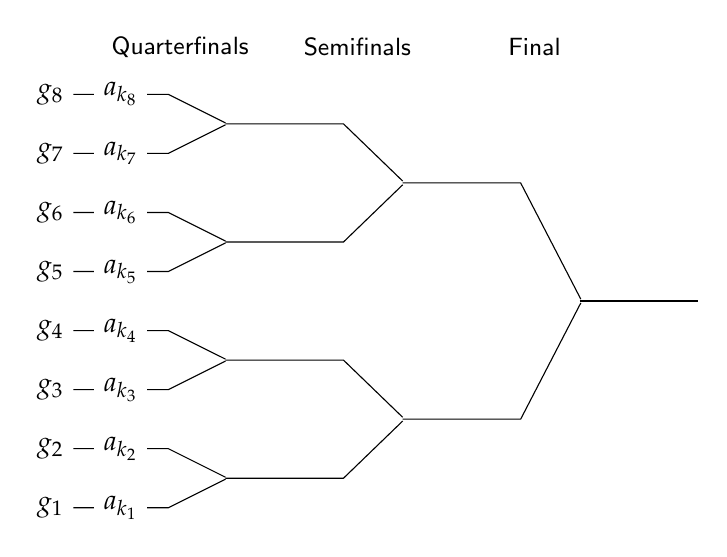
\begin{tikzpicture}[scale=.75]
\foreach \n in {1,2,3,4,5,6,7,8}
  \node (\n) at (0,\n*10mm) {$g_{\n}$};
\foreach \n in {1,2,3,4}
  \node[inner sep=-4pt] (r\n) at (30mm,-5mm+\n*20mm) {};
\foreach \n/\r in {1/1,2/1,3/2,4/2,5/3,6/3,7/4,8/4}
  \draw (\n) --
     node[fill=white] {$a_{k_{\n}}$} +(20mm,0) -- (r\r);
\foreach \n/\v in {1/25mm,2/65mm}
  \node[inner sep=-5pt] (rr\n) at (60mm,\v) {};
\foreach \n/\r in {1/1,2/1,3/2,4/2}
  \draw ($(r\n)+(-1pt,0)$) -- +(20mm,0) -- (rr\r);
\node[inner sep=-5pt] (rrr) at (90mm,45mm) {};
\foreach \n/\r in {1,2}
  \draw ($(rr\n)+(-1pt,0)$) -- +(20mm,0) -- (rrr); 
\draw ($(rrr)+(-1pt,0)$) -- +(20mm,0);
\node at (22mm,88mm) {\textsf{\small Quarterfinals}};
\node at (52mm,88mm) {\textsf{\small Semifinals}};
\node at (82mm,88mm) {\textsf{\small Final}};
\end{tikzpicture}
\end{center}
\caption{A tournament schedule}\label{f.tournament}
\end{figure}

\solution{}

\ans{1}
If $a_1$ is assigned to one of the games $\{g_1,g_2,g_3,g_4\}$ none of the other players assigned to these games will reach the final, so $a_2$ must be assigned to one of $\{g_5,g_6,g_7,g_8\}$. The temptation is to conclude that the probability of $a_2$ being the runner-up is $1/2$ since he must be assigned to one of the four games $\{g_1,g_2,g_3,g_4\}$. However, whatever game $a_1$ is  assigned to, $a_2$ will be the runner up only if he is assigned to one of four of the remaining seven games so the probability is $4/7$.

\ans{2} Similarly, of the $2^n-1$ games that $a_1$ is not assigned to, $a_2$ must be assigned to one of the $2^{n-1}$ games not in the same half as $a_1$. Therefore:
\[
P(a_1,a_2\;\textsf{playing each other in the final})=\frac{2^{n-1}}{2^n-1}\,.
\]

\textbf{Simulation}
\begin{verbatim}
For   8 players:
Probability a2 is runner-up                = 0.5714
Proportion of games where a2 is runner-up  = 0.5707
For  32 players:
Probability a2 is runner-up                = 0.5161
Proportion of games where a2 is runner-up  = 0.5184
For 128 players:
Probability a2 is runner-up                = 0.5039
Proportion of games where a2 is runner-up  = 0.5060
\end{verbatim}

%%%%%%%%%%%%%%%%%%%%%%%%%%%%%%%%%%%%%%%%%%%%%%%%%%%%%%%%%%%%%

\begin{prob}{Twin knights\annotate{D,S}}

Eight players in a tournament $\{a_1,\ldots,a_8\}$ are randomly assigned to play games $\{g_1,\ldots,g_8\}$ in a schedule such that $a_{k_{i}}$ initially plays in position $g_{k_{i}}$ (Figure~\ref{f.tournament}). For all $i,j$, the probability that $a_i$ wins in a game against $a_j$ is $1/2$ as is the probability that $a_j$ wins against $a_i$.

\que{1} What is the probability that $a_1,a_2$ play each other?

\que{2} If there are $2^n$ players, what is the probability that $a_1,a_2$ play each other?
\end{prob}

\solution{}

\ans{1} Without loss of generality assign $a_1$ to $g_1$. Consider the different possibilities that $a_1,a_2$ play each other. With probability $1/7$, $a_2$ is assigned to $g_2$. With probability $2/7$, $a_2$ is assigned to $g_3$ or $g_4$, but he doesn't play $a_1$ unless \emph{both} of them win their first game, so we need to multiply the probability of this assignment by $1/4$. With probability $4/7$, $a_2$ is assigned to $g_5,g_6,g_7,g_8$, but he doesn't play $a_1$ unless \emph{both} of them win their first two  games, so we need to multiply the probability of this assignment by $1/16$. Therefore:
\[
P(a_1, a_2\;\textsf{play each other})=\frac{1}{7} + \frac{1}{4}\cdot \frac{2}{7} + \frac{1}{16}\cdot \frac{4}{7} =\frac{1}{4}\,.
\]

\ans{2}
Let $P_n$ be the probability that in a tournament with $2^n$ players, $a_1$ and $a_2$ play each other. We have shown that $P_3=1/4$. What about $P_4$? Using the same approach:
\begin{eqnarray*}
P_4 &=& \frac{1}{15} + \frac{1}{4}\cdot \frac{2}{15}  + \frac{1}{16}\cdot \frac{4}{15}  + \frac{1}{64}\cdot \frac{8}{15} \\
&=&\frac{1}{15}\left(1+\frac{1}{2}+\frac{1}{4}+\frac{1}{8}\right)=\frac{1}{8}\,.
\end{eqnarray*}
It is reasonable to conjecture that $P_n=1/2^{n-1}$.

\textbf{Proof 1:} Using the same approach and the formula for the sum of a geometric series:
\begin{eqnarray*}
P_n&=&\frac{1}{2^n-1}\sum_{i=0}^{n-1}2^i\cdot \left(\frac{1}{2}\right)^{2i}\\
&=&\frac{1}{2^n-1}\sum_{i=0}^{n-1}2^{-i}\\
&=&\frac{1}{2^n-1}
  \left(
    \frac{1-\left(\frac{1}{2}\right)^{(n-1)+1}}
         {1-\frac{1}{2}}
  \right)=\frac{1}{2^{n-1}}\,.
\end{eqnarray*}

\textbf{Proof 2:} By induction. The base case is $P_3=1/4=1/2^{3-1}$.

There are two inductive steps:

\textit{Case 1:} $a_1$ and $a_2$ are assigned to different halves of the tournament:
\[
P(a_1,a_2\;\textsf{assigned to different halves})=\frac{2^{n-1}}{2^n-1}\,.
\]
They can only meet in the final game and therefore both must win all of their $n-1$ games:
\begin{equation}\label{eq.17a}
P(a_1,a_2\;\textsf{meet if assigned to different halves})=\frac{2^{n-1}}{2^n-1} \left(\frac{1}{2}\right)^{n-1} \left(\frac{1}{2}\right)^{n-1}=\frac{2^{-(n-1)}}{2^n-1}\,.
\end{equation}
\textit{Case 2:} $a_1$ and $a_2$ are assigned to the same half of the tournament:
\[
P(a_1,a_2\;\textsf{assigned to the same half})=\frac{2^{n-1}-1}{2^n-1}\,.
\]
Since both players are in the same half the problem has been reduced to determining $P_{n-1}$. By the inductive hypothesis:
\begin{equation}\label{eq.17b}
P(a_1,a_2\;\textsf{meet if assigned to the same half})=\frac{2^{n-1}-1}{2^n-1}\cdot \frac{1}{2^{n-2}}=\frac{2^{1}-2^{-(n-2)}}{2^n-1}\,.
\end{equation}
Combining Equations~\ref{eq.17a}, \ref{eq.17b} gives:
\[
\renewcommand*{\arraystretch}{2.2}
\begin{array}{rcl}
P_n&=&\disfrac{2^{-(n-1)}}{2^n-1}+\disfrac{2^{1}-2^{-(n-2)}}{2^n-1}\\
&=&\disfrac{2^{n-1}}
        {2^{n-1}}\cdot 
   \disfrac{2^{-(n-1)}+2^{1}-2^{-(n-2)}}
        {2^n-1}\\
&=&\disfrac{1}
        {2^{n-1}}\cdot 
   \disfrac{2^0+2^n-2^1}
        {2^n-1}=\disfrac{1}{2^{n-1}}\,.
\end{array}
\]

\textbf{Simulation}
\begin{verbatim}
For   8 players:
Probability that a1, a2 meet = 0.2500
Proportion a1, a2 meet       = 0.2475
For  32 players:
Probability that a1, a2 meet = 0.0625
Proportion a1, a2 meet       = 0.0644
For 128 players:
Probability that a1, a2 meet = 0.0156
Proportion a1, a2 meet       = 0.0137
\end{verbatim}

%%%%%%%%%%%%%%%%%%%%%%%%%%%%%%%%%%%%%%%%%%%%%%%%%%%%%%%%%%%%%

\begin{prob}{An even split at coin tossing\annotate{S}}
\que{1} If you toss a fair coin $20$ times, what is the probability of obtaining exactly $10$ heads?

\que{2} If you toss a fair coin $40$ times, what is the probability of obtaining exactly $20$ heads?
\end{prob}

\solution{}

\ans{1} Since the coin is fair the probability of obtaining $10$ heads in $20$ tosses is given by the binomial coefficient:
\[
P(10\;\textsf{heads in}\; 20\; \textsf{tosses})={20 \choose 10} \left(\frac{1}{2}\right)^{10}\left(\frac{1}{2}\right)^{10} \approx 0.1762\,.
\]

\ans{2} You might expect the probability to be the same as in the previous question, but:
\[
P(20\;\textsf{heads in}\; 40\; \textsf{tosses})={40 \choose 20} \left(\frac{1}{2}\right)^{20}\left(\frac{1}{2}\right)^{20}\approx 0.1254\,.
\]
By the law of large numbers the numbers of heads and tails will be ``roughly'' equal \cite[Section~8.4]{ross}, but they are unlikely to be exactly the same, and this event becomes less likely as the number of tosses increases.

\textbf{Simulation}
\begin{verbatim}
Probability of 10 heads for  20 tosses = 0.1762
Proportion  of 10 heads for  20 tosses = 0.1790
Probability of 20 heads for  40 tosses = 0.1254
Proportion  of 20 heads for  40 tosses = 0.1212
Probability of 50 heads for 100 tosses = 0.0796
Proportion  of 50 heads for 100 tosses = 0.0785
\end{verbatim}

%%%%%%%%%%%%%%%%%%%%%%%%%%%%%%%%%%%%%%%%%%%%%%%%%%%%%%%%%%%%%

\begin{prob}{Isaac Newton helps Samuel Pepys\annotate{S}}
\que{1} What is the probability of obtaining \emph{at least one} $6$ when $6$ dice are thrown?

\que{2} What is the probability of obtaining \emph{at least two} $6$s when $12$ dice are thrown?

\que{3} Develop a formula for the probability of obtaining at least $n$ $6$s when $6n$ dice are thrown.
\end{prob}

\solution{}

\ans{1} The probability is the complement of the probability of obtain zero $6$s in $6$ throws, which is the product of obtaining a number different from $6$ in all throws:
\[
P(\textsf{at least one}\; 6)=1-\left(\frac{5}{6}\right)^6\approx 0.6651\,.
\]

\ans{2} The probability is the complement of the probability of obtain zero or one $6$s in $12$ throws:
\[
P(\textsf{at least two}\;6\textsf{s})=1-\left(\frac{5}{6}\right)^{12}-{12\choose 1}\left(\frac{1}{6}\right)^{1}\left(\frac{5}{6}\right)^{11}\approx 0.6187\,.
\]
This event is less probable than the previous one.

\ans{3} The probability is the complement of the probability of obtain less than $n$ $6$s in $6n$ throws:
\begin{eqnarray*}
P(\textsf{at least}\;n\;6\textsf{s})&=&
  1-{6n \choose 0}\left(\frac{1}{6}\right)^0\left(\frac{5}{6}\right)^{6n-0}-
  {6n\choose 1}\left(\frac{1}{6}\right)^{1}\left(\frac{5}{6}\right)^{6n-1}-\cdots\\
&=&1-\sum_{i=0}^{n-1}{6n\choose i}\left(\frac{1}{6}\right)^{i}\left(\frac{5}{6}\right)^{6n-i}\,.
\end{eqnarray*}

\textbf{Simulation}
\begin{verbatim}
For   6 dice to throw  1 sixes:
Probability = 0.6651
Proportion  = 0.6566
For  12 dice to throw  2 sixes:
Probability = 0.6187
Proportion  = 0.6220
For  18 dice to throw  3 sixes:
Probability = 0.5973
Proportion  = 0.5949
For  96 dice to throw 16 sixes:
Probability = 0.5424
Proportion  = 0.5425
For 360 dice to throw 60 sixes:
Probability = 0.5219
Proportion  = 0.5250
\end{verbatim}

%%%%%%%%%%%%%%%%%%%%%%%%%%%%%%%%%%%%%%%%%%%%%%%%%%%%%%%%%%%%%

\begin{prob}{The three-cornered duel\annotate{S}}
$A,B,C$ fight a sequence of duels. Each of them has a fixed probability of winning a duel regardless of who the opponent is:
\[
P(A)=0.3,\quad P(B)=1, \quad P(C)=0.5\,.
\]
A person who is hit no longer participates in the duels. The shots are fired one at a time sequentially in the order $A,B,C$. If two opponents are still standing the shooter can decide whom to fire at. Assume that each person always makes an optimal decision.

\que{1} What is $A$'s optimal strategy?

\que{2} Suppose that $A$ fires the first shot into the air. Is this a better strategy?

\textbf{Hint:} Compute the conditional probabilities of $A$ winning depending on whether he chooses to shoot first at $B$ or $C$.
\end{prob}

\solution{}

Notation: $X\stackrel{H}{\longrightarrow}Y$ denotes that $X$ shoots at $Y$ and hits. $X\stackrel{M}{\longrightarrow}Y$ denotes that $X$ shoots at $Y$ and misses.

\ans{1}
Compute the conditional probabilities of $A$ winning.

\textit{Case 1:} $A$ chooses to shoot first at $C$.

If $A\stackrel{M}{\longrightarrow}C$ (probability $0.7$) then $B\stackrel{H}{\longrightarrow}C$ since $C$ is more dangerous than $A$. $A$ now shoots again at $B$ with probability $0.3$ of hitting, but if $A$ misses then $B\stackrel{H}{\longrightarrow}A$ with probability $1$ and $A$ loses.

If $A\stackrel{H}{\longrightarrow}C$ (probability $0.3$) then $B\stackrel{H}{\longrightarrow}A$ with probability $1$ and $A$ loses.

Compute the expectation with $1$ when $A$ wins and $0$ when $A$ loses:
\vspace*{-3ex}
\[
\renewcommand*{\arraystretch}{2.5}
\begin{array}{l}
E(A \;\textsf{wins}\;|A\;\textsf{chooses to shoot first at}\;C) =\\
%\qquad E(A \;\textsf{wins}\;|\;A\;\textsf{misses}\;C) + E(A \;\textsf{wins}\;|\;A\;\textsf{hits}\;C)=\\
\qquad \overbrace{1\cdot (0.7\cdot 0.3)}^{A\stackrel{M}{\longrightarrow}C, A\stackrel{H}{\longrightarrow}B}+ \overbrace{0\cdot (0.7\cdot 0.7\cdot 1)}^{A\stackrel{M}{\longrightarrow}C, A\stackrel{M}{\longrightarrow}B, B\stackrel{H}{\longrightarrow}A}+ \overbrace{0\cdot (0.3\cdot 1)}^{A\stackrel{M}{\longrightarrow}C, B\stackrel{H}{\longrightarrow}A}=0.2100\,.
\end{array}
\]
\textit{Case 2:} $A$ chooses to shoot first at $B$.

If $A\stackrel{M}{\longrightarrow}B$ (probability $0.7$) then as before $B\stackrel{H}{\longrightarrow}C$ and $A$ has one more chance to hit $B$ (probability $0.3$), otherwise $B\stackrel{H}{\longrightarrow}A$ with probability $1$ and $A$ loses.

If $A\stackrel{H}{\longrightarrow}B$ (probability $0.3$) then $A,C$ alternately shoot at each other until one is hit. The possibilities are:
\[
\begin{array}{ll}
(1)&C\stackrel{H}{\longrightarrow}A\\
(2)&C\stackrel{M}{\longrightarrow}A \stackrel{H}{\longrightarrow}C\\
(3)&C\stackrel{M}{\longrightarrow}A \stackrel{M}{\longrightarrow}C\stackrel{H}{\longrightarrow}A\\
(4)&C\stackrel{M}{\longrightarrow}A \stackrel{M}{\longrightarrow}C\stackrel{M}{\longrightarrow}A\stackrel{H}{\longrightarrow}C\\
(5)&C\stackrel{M}{\longrightarrow}A \stackrel{M}{\longrightarrow}C\stackrel{M}{\longrightarrow}A\stackrel{M}{\longrightarrow}C\stackrel{H}{\longrightarrow}A\\
(6)&C\stackrel{M}{\longrightarrow}A \stackrel{M}{\longrightarrow}C\stackrel{M}{\longrightarrow}A\stackrel{M}{\longrightarrow}C\stackrel{M}{\longrightarrow}A\stackrel{H}{\longrightarrow}C\\
&\cdots
\end{array}
\]
The probability of $A$ wins by eventually hitting $C$ is the sum of the probabilities of the even-numbered scenarios in the list:
\begin{eqnarray*}
P(A\;\textsf{wins} \;| A\; \textsf{hits}\;B )&=&(0.5 \cdot 0.3) + \\
&&(0.5 \cdot 0.7) (0.5 \cdot 0.3) + \\
&&(0.5 \cdot 0.7) (0.5 \cdot 0.7) (0.5 \cdot 0.3)+ \cdots\\
&=&0.15 \sum_{i=0}^{\infty} 0.35^i= \frac{0.15}{1-0.35}=\frac{3}{13}\approx 0.2308\,.
\end{eqnarray*}
Similarly, the probability of $C$ winning is $\disfrac{0.5}{1-0.35}=\disfrac{1}{13}\approx 0.0760$.

The expectation is:
\vspace*{-4ex}
\[
\renewcommand*{\arraystretch}{2.5}
\begin{array}{l}
E(A \;\textsf{wins}) =E(A \;\textsf{wins}\;|\;A\;\textsf{misses}\;B) + E(A \;\textsf{wins}\;|\;A\;\textsf{hits}\;B)=\\
\qquad
\overbrace{1\cdot (0.7\cdot 1\cdot 0.3)}%
^{A\stackrel{M}{\longrightarrow}B, B\stackrel{H}{\longrightarrow}C, A\stackrel{H}{\longrightarrow}B}+

\overbrace{0\cdot (0.7\cdot 1\cdot 0.7\cdot 1)}%
^{A\stackrel{M}{\longrightarrow}B, B\stackrel{H}{\longrightarrow}C,A\stackrel{M}{\longrightarrow}B,B\stackrel{H}{\longrightarrow}A} +

\overbrace{1\cdot (0.2308)}%
^{A\stackrel{H}{\longrightarrow}B, C\stackrel{H}{\longleftrightarrow*}A,C\stackrel{H}{\longrightarrow}A} +
\overbrace{0\cdot (0.3\cdot (0.0769))}%
^{A\stackrel{H}{\longrightarrow}B, C\stackrel{H}{\longleftrightarrow}A,C\stackrel{H}{\longrightarrow}A}
\approx\\
\qquad 0.2792\,,
\end{array}
\]
which is higher than the expectation of winning by shooting at $C$ first.

\ans{2} If $A$ shoots into the air not hitting anyone then $B\stackrel{H}{\longrightarrow}C$ with probability $1$ and $A$ can try to hit $B$ with probability $0.3$. The expectation is:
\[
E(A \;\textsf{wins}|A\;\textsf{shoots in the air}) = 1\cdot(0.3) + 0\cdot(0.7)=0.3\,,
\]
which is better than the expectation for the other two strategies!

\textbf{Simulation}
\begin{verbatim}
For A fires first at C:
Expectation of wins = 0.2100
Average wins        = 0.2138
For A fires first at B:
Expectation of wins = 0.2792
Average wins        = 0.2754
For A fires in the air:
Expectation of wins = 0.3000
Average wins        = 0.3000
\end{verbatim}

%%%%%%%%%%%%%%%%%%%%%%%%%%%%%%%%%%%%%%%%%%%%%%%%%%%%%%%%%%%%%

% !TeX root = mos-he.tex

%%%%%%%%%%%%%%%%%%%%%%%%%%%%%%%%%%%%%%%%%%%%%%%%%%%%%%%%%%%%%%%%

\refstepcounter{problem}  % 41. The locomotive problem

%%%%%%%%%%%%%%%%%%%%%%%%%%%%%%%%%%%%%%%%%%%%%%%%%%%%%%%%%%%%%%%%

\begin{prob}{הקצה הקצר של המקל}{}{(The little end of the stick)}

אתה שובר מספר גדול של מקלות זכוכית באורך $1$ לשני חלקים. למקום השבירה התפלגות אחידה לאורך המקל.


\que{1} 
מה התוחלת של אורכו של החלק 
\textbf{הקטן}
יותר?

\que{2} 
מה התוחלת של היחס בין אורכו של החלק הקטן לאורכו של החלק הגדול?
\end{prob}
\solution{}

\ans{1}
ההסתברות שנקודת השבירה היא בצד השמאלי של המקל היא
$1/2$
שהיא גם ההסתברות שהנקודה בצד ימין. החלק הקטן יותר נמצא באותו צד שבו נמצאת נקודת השבירה. התוחלת של נדוקת השבירה היא באמצע בין קצה המקל לבין אמצע המקל:
\[
E(\textrm{יותר הקטן אורך}) = \frac{1}{2}\cdot\frac{1}{2}=\frac{1}{4}\,.
\]

\ans{2}
ללא הגבלת הכלליות הנח שנקודת השבירה נמצאת בצד הימני של המקל (איור%
~\ref{f.stick}).
היחס בין החלק הקטן והחלק הגדול הוא
$(1-x)/x$
ואורכו של החלק הגדול מתפלג אחיד בתוך
$(1/2,1)$. 
לכן:
\begin{eqn}
E(\textrm{יותר קטן / יותר גדול יחס})&=&\left(\frac{1}{1-(1/2)}\right)\int_{1/2}^1 \frac{1-x}{x} \,dx\\
&=& 2\int_{1/2}^1 \left(\frac{1}{x} -1\right) \,dx \\
&=& 2\left.(\ln |x| - x)\right|_{1/2}^1 = 2\ln 2 -1\approx 0.3863\,.
\end{eqn}
\begin{figure}[tb]
\begin{center}
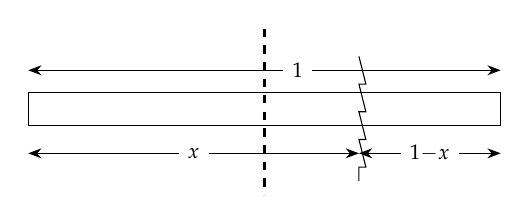
\begin{tikzpicture}
\draw (0,0) -- ++(6,0) -- ++(0,12pt) -- ++(-6,0) -- cycle;
\draw[<->] (0,20pt) --
  node[fill=white,xshift=12pt] {$\scriptstyle 1$} ++(6,0);
\draw[decorate,decoration=saw] (4.2,25pt) -- +(0,-45pt);
\draw[thick,dashed] (3,35pt) -- +(0,-60pt);
\draw[<->] (0,-10pt) --
  node[fill=white] {$\scriptstyle x$} (4.2,-10pt);
\draw[<->] (4.2,-10pt) --
  node[fill=white] {$\scriptstyle 1-x$} (6,-10pt);
\end{tikzpicture}
\end{center}
\caption{שבירת מקל לשני חלקים}\label{f.stick}
\end{figure}

\textbf{סימולציה}
\selectlanguage{english}
\begin{verbatim}
Expectation of length of smaller = 0.2500
Average length of smaller        = 0.2490
Expectation of smaller/larger    = 0.3863
Average smaller/larger           = 0.3845
\end{verbatim}
\selectlanguage{hebrew}

%%%%%%%%%%%%%%%%%%%%%%%%%%%%%%%%%%%%%%%%%%%%%%%%%%%%%%%%%%%%%%%%


\begin{prob}{המקל השבור}{D}{(The broken bar)}

אתה שובר מספר רב של מקלות זכוכית באורך 
$1$
בשתי נדוקות שבירה (איור%
~\ref{f.break1}).

\que{1} 
מה התוחלת של אורכו של החלק הקצר ביותר?

\que{2} 
מה התוחלת של אורכו של החלק הארוך ביותר?

\textbf{רמז:}
$x,y$
הם משתנים אקראים בלתי-תלויים בהתפלגות אחידה בתוך 
$(0,1)$.
ניתן להציג כל זוג
$(x,y)$
כנקודה בריבוע
$(0,1)\times (0,1)$ 
(איור%
~\ref{f.break2}).
מה ההסתברות ש-%
$(x,y) < (.5,.25)$? 

\textbf{Hint:}
עבור 
\que{1}
הנח שהחלק השמאלי הוא הקצר ביותר ועבור 
\que{2}
הנח שהחלק השמאלי הוא בארוך ביותר.
\begin{figure}[tb]
\centering
\selectlanguage{hebrew}
\subcaptionbox{%
חלוקת מקל לשני חלקים%
\label{f.break1}}
[.45\textwidth]
{
\centering
\begin{tikzpicture}[scale=.75]
\draw (0,0) node[below left] {$0$} --
  ++(6,0) node[below right] {$1$} --
  ++(0,12pt) -- ++(-6,0) -- cycle;
\draw[<->] (0,20pt) --
  node[fill=white] {$\scriptstyle 1$} ++(6,0);
\draw[decorate,decoration=saw] (1.8,25pt) -- +(0,-45pt);
\draw[decorate,decoration=saw] (4.7,25pt) -- +(0,-45pt);
\node[below left] at (1.8,0) {$x$};
\node[below left] at (4.7,0) {$y$};
\path (0,-3.5) rectangle +(0,3.5);
\end{tikzpicture}
}
\hspace{3em}
\subcaptionbox{%
יצוג האורכים במעגל היחידה%
\label{f.break2}}
[.45\textwidth]
{
\centering
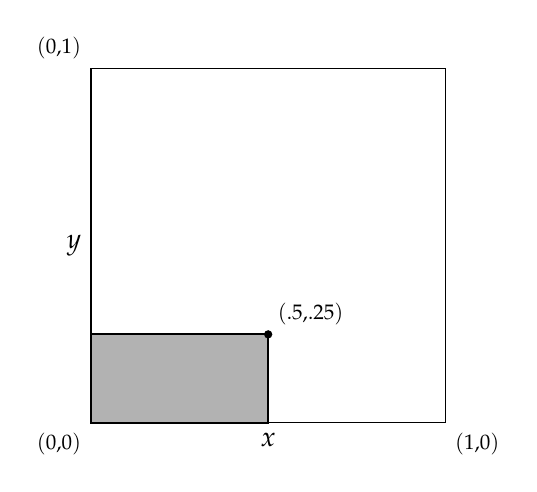
\begin{tikzpicture}[scale=.75]
\draw (-3,-3) rectangle +(6,6);
\draw[thick,fill=white!70!black] (-3,-3) -- ++(0,1.5) -- 
  ++(3,0) -- ++(0,-1.5) -- cycle;
\path (-3,-3) node[below left] {$\scriptstyle (0,0)$} --
  node[below] {$x$} (3,-3)
  node[below right] {$\scriptstyle (1,0)$};
\path (-3,-3) -- node[left] {$y$} (-3,3)
  node[above left] {$\scriptstyle (0,1)$};
\fill (0,-1.5) circle [radius=2pt]
  node[above right] {$\scriptstyle (.5,.25)$};
\end{tikzpicture}
}
\end{figure}
\end{prob}
\solution{}

\ans{1}
ללא הגבלת הכלליות הנח שהחלק השמאלי שאורכו 
$x$
הוא החלק הקצר ביותר. מכאן ש-%
$x<y-x$
ו-%
$x < 1-y$
שניתן לפשט ולקבל
$2x<y$
ו-%
$x+y<1$.

איור%
~\ref{f.shaded1}
מראה את הקווים
$y=2x$
(אדום) ו-%
$y=1-x$
(כחול). כדי לאמת את אי-השוויונות, 
$(x,y)$
חייבת להיות באיזור באפור לשמאל לשני הקווים. ניתן לחשב את נקודת החיתוך
$(1/2,2/3)$
על ידי פתרון שתי המשוואות.

הערכים של 
$(x,y)$
נמצאים בריבוע
$(0,1)\times(0,1)$,
ולכן יש לחשב את התוחלת מעל לתת-קבוצה האפורה של הריבוע על ידי חילוק האינטגרל בשטח של האיזור האפור
$\frac{1}{2} (\frac{1}{3}\cdot 1)=\frac{1}{6}$:
\begin{eqn}
E(x)&=& \frac{1}{1/6}\int_{0}^{1/3} x [(1-x)-2x]\,dx\\
&=&\int_{0}^{1/3} (6x -18x^2)\,dx\\
&=&\left. (3x^2-6x^3)\right|_0^{1/3}=\disfrac{2}{18}\approx 0.1111\,.
\end{eqn}

\begin{figure}[tb]
\centering
\selectlanguage{hebrew}
\subcaptionbox{%
איזור אפור עבור המקל הקצר ביותר%
\label{f.shaded1}}
[.45\textwidth]
{
\centering
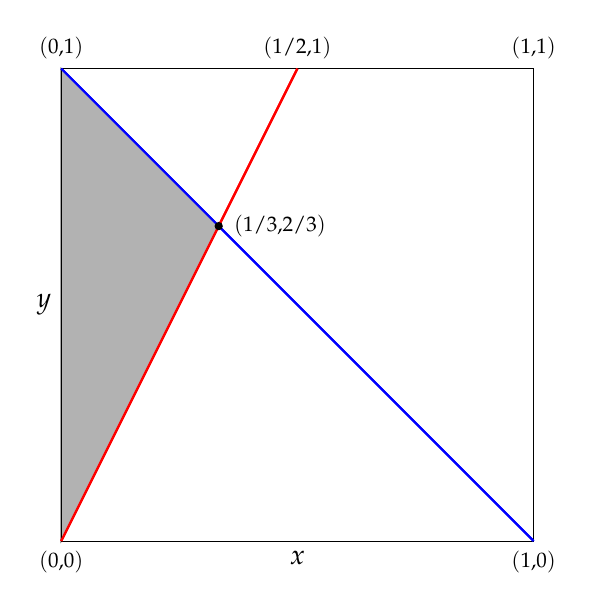
\begin{tikzpicture}[scale=1]
\draw (-3,-3) rectangle +(6,6);
\path (-3,-3) node[below] {$\scriptstyle (0,0)$} --
  node[below] {$x$} (3,-3)
  node[below] {$\scriptstyle (1,0)$};
\path (-3,-3) -- node[left] {$y$} (-3,3)
  node[above] {$\scriptstyle (0,1)$};
\draw[red,thick]  (-3,-3) -- (0,3);
\draw[blue,thick] (-3,3)  -- (3,-3);
\coordinate (P) at (-1,1);
\draw[fill=white!70!black] (-3,-3) -- (P) -- 
  (-3,3) -- cycle;
\draw[red,thick]  (-3,-3) -- (0,3);
\draw[blue,thick] (-3,3)  -- (3,-3);
\fill (P) circle[radius=1.5pt]
  node[right,xshift=2pt] {$\scriptstyle (1/3,2/3)$};
%\draw[thick,dotted] (-3,-3) -- (3,3);
\node[above] at(0,3) {$\scriptstyle (1/2,1)$};
\node[above] at(3,3) {$\scriptstyle (1,1)$};
\end{tikzpicture}
}
\hspace{1em}
\subcaptionbox{%
איזור אפור עבור המקל הארוך ביותר%
\label{f.shaded2}}
[.45\textwidth]
{
\centering
\begin{tikzpicture}[scale=1]
\draw (-3,-3) rectangle +(6,6);
\path (-3,-3) node[below] {$\scriptstyle (0,0)$} --
  node[below] {$x$} (3,-3)
  node[below] {$\scriptstyle (1,0)$};
\path (-3,-3) -- node[left] {$y$} (-3,3)
  node[above] {$\scriptstyle (0,1)$};
\coordinate (P) at (-1,1);
\coordinate (Q) at (0,0);
\draw[fill=white!70!black] (3,3) -- (Q) -- 
  (P) -- (0,3) -- cycle;
\draw[red,thick]  (-3,-3) -- (0,3);
\draw[blue,thick] (-3,3)  -- (3,-3);
\fill (P) circle[radius=1.5pt]
  node[left,xshift=-2pt] {$\scriptstyle (1/3,2/3)$};
\draw[thick,dotted] (-3,-3) -- (3,3);
\fill (Q) circle[radius=1.5pt]
  node[right,xshift=2pt] {$\scriptstyle (1/2,1/2)$};
\node[above] at(0,3) {$\scriptstyle (1/2,1)$};
\node[above] at(3,3) {$\scriptstyle (1,1)$};
\draw[thick,dashed] (Q) -- ++(0,3);
\draw (0,3cm-7pt) rectangle +(7pt,7pt);
\end{tikzpicture}
}
\end{figure}

\ans{2}
כדי שהחלק השמאלי יהיה הארוך ביותר 
$x>y-x$
ו-%
$x>1-y$, 
ולכן
$(x,y)$
חייבת להיות לימינו של
$y=2x$
(אדום) ולימינו של
$y=1-x$
(כחול) (איור%
~\ref{f.shaded2}).
בנוסף, לפי הנחה ש-%
$x$
נמצא לשמאלו של
$y$,
$(x,y)$
חייבת להיות לשמאלו של
$y=x$
(מנוקד).

כדי להקל על החישוב נחלק את האיזור האפור לשני משולשים (מקווקו) ונחשב את התוחלת בנפרד בשניהם. השטח של האיזור האפור מתקבל כסכום השטחים של המשולשים
$1/24+1/8=1/6$.
מכאן:
\begin{eqn}
E(\textrm{השמאלי במשולש}\;x)&=& 6\int_{1/3}^{1/2} x [2x-(1-x)]\,dx  \\
&=&\int_{1/3}^{1/2} \left(18x^2-6x\right)\,dx\\
&=&\left. (6x^3-3x^2)\right|_{1/3}^{1/2}=\disfrac{1}{9}\\
E(\textrm{הימני במשולש}\;x)&=& 6\int_{1/2}^{1} x [1-x]\,dx\\
&=&\int_{1/2}^{1} (6x-6x^2)\,dx\\
&=&\left. \left(3x^2-2x^3\right)\right|_{1/2}^{1}= \disfrac{1}{2}\\
E(x)&=& \disfrac{1}{9}+\disfrac{1}{2} = \disfrac{11}{18}\approx 0.6111\,.
\end{eqn}

התוחלת של אורכו של החלק הבינוני היא
$1-\frac{2}{18}-\frac{11}{18}=\frac{5}{18}\approx 0.2778$.

\textbf{סימולציה}
\selectlanguage{english}
\begin{verbatim}
Expectations: shortest = 0.1111, middle = 0.2778, longest = 0.6111
Averages:     shortest = 0.1115, middle = 0.2783, longest = 0.6102
\end{verbatim}
\selectlanguage{hebrew}

%%%%%%%%%%%%%%%%%%%%%%%%%%%%%%%%%%%%%%%%%%%%%%%%%%%%%%%%%%%%%%%%

\begin{prob}{לנצח במשחק לא-הוגן}{D}{(Winning an unfair game)}

נתון מטבע לא-הוגנת שההסתברות לעץ היא 
$1/3 < p < 1/2$. 
הטל את המטבע מספר זוגי של פעמים
$N=2n$.
אתה מנצח אם ורק אם 
\textbf{ביותר}
ממחצית ההטלטת מופיע עץ.

\que{1}
פתח נוסחה עבור ההסתברות לנצח 
$P_N$
ונוסחה עבור ההסתברות לתיקו
$T_N$.

\que{2}
פתח נוסחה עבור ה-%
$N$
עבורו יש את ההסתברות הגבוהה ביותר לנצח.

\textbf{רמז:} 
אם ההסתברות הגבוהה ביותר לנצח היא ב-%
$N$
הטלות אזי 
$P_{N-2} \leq P_N$
ו-%
$P_N\geq P_{N+2}$.
\end{prob}
\solution{}

\ans{1} 
כדי לנצח, עץ חייב להופיע ב-%
$i\in\{n+1, n+2, \ldots, 2n-1, 2n=N\}$
הטלות. מההתפלגות הבינומית:
\begin{eqn}
P_N &=& \sum_{i=n+1}^{2n} \dischoose{2n}{i} p^i (1-p)^{2n-i}\\
T_N &=& \dischoose{2n}{n} p^n (1-p)^{n}\,.
\end{eqn}

\ans{2}
כדי שההסתברות הגבוהה ביותר תהיהעבור
$N=2n$
חייב להתקיים:
\[
P_{2n-2} \leq P_{2n} \quad \textrm{ו-} \quad P_{2n}\geq P_{2n+2}\,.
\]
מתי
$P_{2n-2}\not = P_{2n}$?

\textbf{מקרה 1:}
לאחר הטלה
$2n-2$,
עץ הופיע 
$n$
פעמים ופלי
$n-2$
פעמים (כך שהיית זוכה אם היית עוצר כאן), אבל פלי מופיע בשתי ההטלות הבאות. עכשיו יש
$n$
עץ ו-%
$n$
פלי ולכן אתה מפסיד. ההסתברות היא:
\[
\dischoose{2n-2}{n}p^n(1-p)^{n-2} (1-p)^2\,.
\]

\textbf{מקרה $2$:}
לאחר הטלה
$2n-2$,
עץ הופיע 
$n-1$
פעמים ופלי
$n-1$
פעמים (כך שהיית מפסיד אם היית עוצר כאן), אבל עץ מופיע בשתי ההטלות הבאות. עכשיו יש
$n+1$
עץ ו-%
$n-1$
פלי ולכן אתה מנצח. ההסתברות היא:
\[
\dischoose{2n-2}{n-1}p^{n-1}(1-p)^{n-1} p^2\,.
\]
כדי לאמת את
$P_{2n-2}\leq P_{2n}$,
$P_{2n-2}$
לא יכול לגדול כאשר 
$P_{2n}$
נשאר ללא שינוי (מקרה $1$), אבל 
$P_{2n}$
יכול לגבול עד שהיא גבוהה מ-%
$P_{2n-2}$ (מקרה 2).
לכן:
\begin{eqn}
\dischoose{2n-2}{n}p^n(1-p)^{n-2} (1-p)^2 &\leq&
\dischoose{2n-2}{n-1}p^{n-1}(1-p)^{n-1} p^2\\
\disfrac{1}{n} (1-p) &\leq& \disfrac{1}{n-1} p\\
(n-1)(1-p) &\leq& np\\
n &\leq& \disfrac{1-p}{1-2p}\\
2n &\leq& \disfrac{1}{1-2p}+1\,.
\end{eqn}
באופן דומה, כדי לאמת את
$P_{2n}\geq P_{2n+2}$
חייב להיול ש:
\begin{eqn}
\dischoose{2n}{n+1}p^{n+1}(1-p)^{n-1}  (1-p)^2 &\geq&
\dischoose{2n}{n}p^{n}(1-p)^{n}  p^2\\
\disfrac{1}{n+1} (1-p) &\geq& \disfrac{1}{n} p\\
n(1-p)&\geq& (n+1)p\\
n &\geq& \disfrac{p}{1-2p}\\
2n &\geq&\disfrac{1}{1-2p}-1\,.
\end{eqn}
לכן, ערך עבור
$N=2n$
שעבורו מתקבל ההסתברות הגבוהה ביותר הוא המספר השלם הזוגי הקרוב ביותר ל-%
$1/(1-2p)$.
הקורא מוזמן להראות שאם
$1/(1-2p)$
אי-זוגי אזי
$P_{2n}=P_{2n+2}$.

\textbf{סימולציה}
\selectlanguage{english}
\begin{verbatim}
For probability             = 0.3700
Optimal games to be played  = 4
For  2 games, average won   = 0.1372
For  4 games, average won   = 0.1445
For  6 games, average won   = 0.1431

For probability             = 0.4000
Optimal games to be played  = 6
For  4 games, average won   = 0.1820
For  6 games, average won   = 0.1845
For  8 games, average won   = 0.1680

For probability             = 0.4500
Optimal games to be played  = 10
For  8 games, average won   = 0.2671
For 10 games, average won   = 0.2646
For 12 games, average won   = 0.2640
\end{verbatim}
\selectlanguage{hebrew}

%%%%%%%%%%%%%%%%%%%%%%%%%%%%%%%%%%%%%%%%%%%%%%%%%%%%%%%%%%%%%%%%

\begin{prob}{ממוצע של מספר ההתאמות}{}{(Average number of matches)}
סדר חפיסת קלפים בשורה בסדר הסטנדרטי ואז סדר חפיסה שניה שורה בסדר אקראי מתחת לשורה הראשונה (איור%
~\ref{f.cards}).
מה התוחלת של מספר ההתאמות של קלף בשורה הראשונה עם קלף בשורה מתחתיו?
\end{prob}
\begin{figure}[tb]
\begin{center}
\begin{tikzpicture}
\foreach \x/\v/\s in {
  0/A/\spadesuit,
  1/2/\spadesuit,
  2.25/\cdots/,
  3.5/K/\spadesuit,
  4.5/A/\heartsuit,
  5.5/2/\heartsuit,
  6.75/\cdots/,
  8/K/\heartsuit,
  9/A/\diamondsuit,
  10/2/\diamondsuit,
  11.25/\cdots/,
  12.5/K/\diamondsuit,
  13.5/A/\clubsuit,
  14.5/2/\clubsuit,
  15.75/\cdots/,
  17/K/\clubsuit}
  \node[minimum height=9mm,draw,rounded corners]
    at (\x*24pt,0) {\shortstack{$\v$\\$\s$}};

\foreach \x/\v/\s in {
  0/J/\clubsuit,
  1/2/\spadesuit,
  2.25/\cdots/,
  3.5/7/\heartsuit,
  4.5/4/\diamondsuit,
  5.5/2/\heartsuit,
  6.75/\cdots/,
  8/K/\heartsuit,
  9/8/\clubsuit,
  10/Q/\spadesuit,
  11.25/\cdots/,
  12.5/4/\spadesuit,
  13.5/8/\heartsuit,
  14.5/A/\clubsuit,
  15.75/\cdots/,
  17/K/\clubsuit}
  \node[minimum height=9mm,draw,rounded corners]
    at (\x*24pt,-50pt) {\shortstack{$\v$\\$\s$}};

\node at (24pt,-25pt) {$\updownarrow$};
\node at (133pt,-25pt) {$\updownarrow$};
\node at (193pt,-25pt) {$\updownarrow$};
\node at (410pt,-25pt) {$\updownarrow$};
\end{tikzpicture}
\end{center}
\caption{התאמת שתי חפיסות קלפים}\label{f.cards}
\end{figure}
\solution{}

ההתפלגות אחידה כי לכל קלף בשורה השניה אותה המסתברות להתאים לקלף מעליו. לכן:
\[
E(\textrm{ההתאמות מספר}) = 52\cdot \frac{1}{52} = 1\,.
\]
\selectlanguage{english}
\begin{verbatim}
Expectation of matches = 1.00
Average of matches     = 1.01
\end{verbatim}
\selectlanguage{hebrew}

%%%%%%%%%%%%%%%%%%%%%%%%%%%%%%%%%%%%%%%%%%%%%%%%%%%%%%%%%%%%%%%%

\begin{prob}{הסתברויות של התאמות}{}{(Probabilities of matches)}

סדר חפיסת קלפים בשורה בסדר הסטנדרטי ואז סדר חפיסה שניה שורה בסדר אקראי מתחת לשורה הראשונה (איור%
~\ref{f.cards}).
פתח נוסחה עבור 
$P(n,r)$,
ההסתברות שיהיו בדיוק 
$r$
התאמות של קלף בשורה הראשונה עם קלף בשורה מתחתיו? הנח ש-%
$P(k,0)$
נתון עבור
$0\leq k\leq n$.
\end{prob}
\solution{}

במבט ראשון נראה שבעיה זו דומה לבעיה~28 אבל קיים הבדל מהותי. השליפות המקופסאות הן בלתי-תלויות אבל כאן ההתאמות תלויות אחת בשניה. למשל, אם יש התאמה בקלף הראשון (בהסתברות 
$1/n$),
ההסתברות של התאמה בקלף השני היא
$1/(n-1)$.

ההסתברות שקבוצה 
\textbf{נתונה}
של
$r$
קלפים מתאימות היא:
\begin{equation}\label{eq.r-match}
\disfrac{1}{n}\cdot \disfrac{1}{n-1}\cdot \cdots \cdot \disfrac{1}{n+r-1}\,.
\end{equation}
כדי לקבל בדיוק 
$r$
התאמות, יש להכפיל משוואה%
~\ref{eq.r-match}
ב-%
$P(n-r,0)$,
ההסתברות שאין בכלל התאמות בשאר 
$n-r$
הקלפים. לבסוף, יש 
${n\choose r}$
דרכים לבחור
$r$
התאמות, ולכן:
\begin{eqn}
P(n,r)&=& \dischoose{n}{r}\disfrac{1}{n(n-1)(n+r-1)} P(n-r,0)\\
&=& \disfrac{n!}{r!(n-r)!}\cdot\disfrac{1}{n!/(n-r)!}P(n-r,0)\\
&=&\disfrac{1}{r!}P(n-r,0)\,.
\end{eqn}
נוסחה זו פותרת את הבעיה כי 
$P(k,0)$
נתונה.

\L{Mosteller}
מפתח נוסחה סגורה וגבול עבור
$P(n,r)$:
{
\addtolength{\arraycolsep}{-3pt}
\begin{eqnarray}
P(n,k)&=&\disfrac{1}{k!}\sum_{i=0}^{n-k} \disfrac{(-1)^i}{i!}\\
\label{eq.r-matches-lim}
\lim_{n-r\rightarrow \infty} P(n,k)&\approx& \disfrac{1}{k!}e^{-1}\,.
\end{eqnarray}
}

\textbf{סימולציה}

הרצתי את הסימולציה עבור 
$n=52$
קלפים וחישבתי את ההסתברות ממשוואה%
~\ref{eq.r-matches-lim}.
\selectlanguage{english}
\begin{verbatim}
Probability of 1 matches = 0.3679
Proportion 1 matches     = 0.3710
Probability of 2 matches = 0.1839
Proportion 2 matches     = 0.1828
Probability of 3 matches = 0.0613
Proportion 3 matches     = 0.0569
Probability of 4 matches = 0.0153
Proportion 4 matches     = 0.0168
\end{verbatim}
\selectlanguage{hebrew}

%%%%%%%%%%%%%%%%%%%%%%%%%%%%%%%%%%%%%%%%%%%%%%%%%%%%%%%%%%%%%%%%

\begin{prob}{לבחור את הנדוניה הגדול ביותר}{D}{(Choosing the largest dowry)}

הנח סידרה של 
$n$
קלפים עם הפנים למטה. על פניו של כל קלף נמצא מספר שלם חיובי אבל אין מידע על ההתלפגות שלהם. הפוך את הקלפים אחד-אחד ועיין במספרים. לאחר חשיפת כל אחד מהקלפים, אתה יכול להכריז שמספר זה הוא הגדול ביותר בסידרה. אם אתה צודק אתה מנצח, אחרת אתה מפסיד. למשל, אם הסדרה היא 
$(47, 23, 55, 4)$,
אתה מנצח רק אם אתה בוחר שת הקלף השלישי.

הנה אסטרטגיה: ל-%
$r$
קבוע, וותר על
$r-1$
הקלפים הראשונים ובחר את הקלף הראשון שמספרו גדול מכל 
$r-1$
הקלפים.

\que{1}
עבור
$n=4$
ו-%
$r=3$
בדוק את כל התמורות ומצא בכמה מהם את מנצח.

\que{2}
פתח נוסחה עבור ההסתברות לניצחון עבור 
$n, r$
שרירותיים.

\que{3} מצא קירוב להסתברות כאשר 
$n,r\rightarrow \infty$.

\textbf{רמז:}
נתון
$r$
באיזה מקומות יכול להופיע המספר הגדול ביותר
$m$
ובאיזה מקומות המספרים שהם פחות או שווים ל-%
$m$? 

\end{prob}
\solution{}

\ans{1}
כדי לפשט את הסימון נכתוב את דירוג מספרים כ-%
$1,2,3,4$
למרות שהערכים אמיתיים של המספרים לא ידועים, ולמשל יכולים להיות 
$4,23,47,55$.
אם אתה חושף קלפים
$1,2,3$
(שהם בעצם
$4,23,47$),
אינך יודע אם לבחור
$47$
או לחכות ובחור את הקלף האחרון.

יש 
$24$
תמורות של ארבעה מספרים. לפי האסטרטגיה אתה מוותר על שני הקלפים הראשונים ובוחר או את הקלף השלישי או את הקלף הרביעי, כך שאתה מפסיד אם $4$ נמצא במקום הראשון של התמורה. מה עם התמורה
$(1,2,3,4)$?
אתה מוותר על
$1,2$
ובוחר 
$3$
בגלל שהוא גובהה יותר מ-%
$1,2$
אבל אתה מפסיד כי זה לא המספר הגדולה ביותר. מה עם התמורה
$(1,3,2,4)$?
שוב, לפי האסטרטגיה אתה מוותר על
$1,3$,
אבל מוותר גם על
$2$
כי הוא 
\textbf{לא}
גדול יותר מ-%
$1,3$.
כעת אתה בוחר
$4$
ומנצח. נסח טיעונים דומים לכל התמורות ובדוק שכל התמורות עם 
$4$
במסגרת הן נצחונות:
\[
\addtolength{\arraycolsep}{-2pt}
\renewcommand*{\arraystretch}{1.5}
\begin{array}{cc|cc@{\hspace{2em}}cc|cc@{\hspace{2em}}cc|cc@{\hspace{2em}}cc|cc@{\hspace{2em}}cc|cc@{\hspace{2em}}cc|cc}
1&2\;&\;3&4&
1&2\;&\;\fbox{$4$}&3&
1&3\;&\;2&\fbox{$4$}&
1&3\;&\;\fbox{$4$}&2&
1&4\;&\;2&3&
1&4\;&\;3&2\\
2&1\;&\;3&4&
2&1\;&\;\fbox{$4$}&3&
2&3\;&\;1&\fbox{$4$}&
2&3\;&\;\fbox{$4$}&1&
2&4\;&\;1&3&
2&4\;&\;3&1\\
3&1\;&\;2&\fbox{$4$}&
3&1\;&\;\fbox{$4$}&2&
3&2\;&\;1&\fbox{$4$}&
3&2\;&\;\fbox{$4$}&1&
3&4\;&\;2&1&
3&4\;&\;2&1\\
4&1\;&\;2&3&
4&1\;&\;3&2&
4&2\;&\;1&3&
4&2\;&\;3&1&
4&3\;&\;1&2&
4&3\;&\;2&1
\end{array}
\]
ההסתברות לנצח היא
$10/24$.

\ans{2}
אתה מפסיד אם המספר הגדול ביותר נמצא באחד המקומות
$1,\ldots,r-1$.
לכן כדי לנצח מספר הגדול ביותר חייב להיות במקום
$m$
כאשר
$r\leq m\leq n$:
\[
1\quad 2\quad \cdots\quad r-2 \quad r-1 \quad \overbrace{r \quad r+1 \quad \cdots\quad m-1\quad  m \quad m+1\quad \cdots \quad n}^{\textrm{כאן להיות חייב ביותר גדול מספר}}\,.
\]
לפי האסטרטגיה אתה מוותר על
$r-1$
הקלפים הראשונים. אתה תבחר מקום
$m$
אם ורק אם 
\textbf{כל}
במספרים ב-%
$(r,\ldots,m-1)$
קטנים מ%
\textbf{כל}
המספרים ב-%
$(1,\ldots,r)$.
במילים אחרות, המספר הגדול ביותר בסידרה
$(1,\ldots,m-1)$
הוא
\textbf{לא}
בחלק השני של הסידרה
$(r,\ldots m-1)$
אלא בחלק הראשון
$(1,\ldots,r-1)$.
ההסתברות היא:
\[
P((1,\ldots,r-1)\textrm{ב- נמצא}\;(1,\ldots,m-1)\textrm{ב- ביותר הגדול המספר}) = \disfrac{r-1}{m-1}\,.
\]
ההסתברות שהמספר הגדול ביותר נמצא ב-%
$m$
הוא
$1/n$
ולכן:
\begin{equation}\label{eq.dowry1}
P(\textrm{ניצחון}) = \sum_{m=r}^{n} \disfrac{1}{n} \cdot \disfrac{r-1}{m-1}= \disfrac{r-1}{n}\sum_{m=r}^{n} \disfrac{1}{m-1}\,.
\end{equation}
עבור
$n=4, r=3$, $P(\textrm{ניצחון}) = 5/12=10/24$.

משוואה%
~\ref{eq.dowry1}
לא מוגדרת עבור
$r=1$
אבל ההסתברות לנצח כאשר אתה בוחר את המספר הראשון הוא
$1/n$.
לערך גבוהה ביותר של
$r$
יש הסתברות גבוהה יותר כפי שראינו בדוגמה.

\ans{3}
נכתוב משוואה%
~\ref{eq.dowry1}
כך:
\begin{equation}\label{eq.dowry2}
P(\textrm{ניצחון}) =\disfrac{r-1}{n}\left(\sum_{m=2}^{n} \disfrac{1}{m-1}-\sum_{m=2}^{r-1} \disfrac{1}{m-1}\right)\,.
\end{equation}
עבור 
$n,r$
גדולים, ניתן למצוא קירוב למשוואה%
~\ref{eq.dowry2}
כך:
\[
P(\textrm{ניצחון})=\disfrac{r}{n}(\ln n - \ln r)=\disfrac{r}{n}\ln \disfrac{n}{r}=-\disfrac{r}{n}\ln \disfrac{r}{n}\,.
\]
נסמן
$x=r/n$
ונמצא את המקסימום מהנגזרת:
\begin{eqn}
(-x\ln x)' &=& -x\cdot \frac{1}{x} + (-1) \ln x=0\\
\ln x &=& -1\\
x &=& 1/e\,.
\end{eqn}
כדי למקסם את ההסתברות לנצח בחר
$r \approx n/e$.

\textbf{סימולציה}

הרצתי את הסימולציה עם
$100$
קלפים וערכי
$r$
קרובים ל-%
$100/e$:
\selectlanguage{english}
\begin{verbatim}
Reject cards before r = 36:
Probability of wins   = 0.3674
Proportion wins       = 0.3641
Reject cards before r = 37:
Probability of wins   = 0.3678
Proportion wins       = 0.3759
Reject cards before r = 38:
Probability of wins   = 0.3679
Proportion wins       = 0.3548
Reject cards before r = 30:
Probability of wins   = 0.3590
Proportion wins       = 0.3601
\end{verbatim}
\selectlanguage{hebrew}

%%%%%%%%%%%%%%%%%%%%%%%%%%%%%%%%%%%%%%%%%%%%%%%%%%%%%%%%%%%%%%%%

\begin{prob}{בחירת המספר האקראי הגדול ביותר}{D}{(Choosing the largest random number)}

הנח סידרה של 
$n$
קלפים עם הפנים למטה. על פניו של כל קלף נמצא מספר ממשי עם התפלגות אחידה ב-%
$0.0\leq x<1.0$.
הפוך את הקלפים אחד-אחד ועיין במספרים. לאחר חשיפת כל אחד מהקלפים, אתה יכול להכריז שמספר זה הוא הגדול ביותר בסידרה. אם אתה צודק אתה מנצח, אחרת אתה מפסיד.

השתמש באסטרטגיה של בעיה~37: החלט על ערך
$r$
כך שאתה מוותר על 
$r-1$
הקלפים הראשונים ובוחר את הקלף הראשון שגדול מהמספר הגדול ביותר ב-%
$r-1$
קלפים הראשונים.

\textbf{הגדרה:}
$d$,
\textbf{ערך שווה-נפש},
הוא הערך שמתחתיו אתה מוותר על הקלף ומעליו את לבחור את הקלף.

\que{1} 
חשב את
$d$
עבור
$n=1$
וחשב את ההסתברות לנצח.

\que{2}
חשב את
$d$
עבור
$n=2$
וחשב את ההסתברות לנצח.

\que{3}
חשב את
$d$
עבור
$n=3$.
אל תנסה לחשב את ההסתברות לנצח!

\textbf{הערה:}
בבעיה~37 בערכים יכולים להיות
$100, 200, 300$ 
או
$100, 50, 20$
כך שחשיפת המספר הראשון לא מספק שום מידע על המספרים האחרים. בבעיה זו, ההתלפגות אחידה, ולכן אם המספר הראשון הוא 
$0.2$,
ההסתברות שהמספר השני יהיה גדול יותר היא 
$0.8$
ואם המספר הראשון הוא 
$0.8$
ההסתברות שהמספר השני יהיה גדול יותר היא
$0.2$.

\end{prob}
\solution{}

יהי
$v_1,v_2,v_3$
המספרים על שלושת הכרטיסים.

\ans{1}
אין ברירה אלא לבחור את הקלף הראשון כי אין קלפים אחרים. לכן אין ערך שווה-נפש. 
$v_1$
הוא המספר "הגדול ביותר",
$P(\textrm{ניצחון})=1$.

\ans{2}
אם אתה בוחר את הקלף הראשון
$P(\textrm{ניצחון})=v_1$
שהיא ההסתברות שהמספר על הקלף השני קטן יותר. אם אתה מוותר על הקלף הראשון,
$P(\textrm{ניצחון})=1-v_1$
שהיא ההסתברות ש-%
$v_2>v_1$.
לכן, אם 
$v_1<0.5$ 
בחר את הקלף השני כי
$1-v_1>0.5$
ואם 
$v_1>0.5$
בחר את הקלף הראשון. מכאן ש-%
$d=0.5$.

הנה הנוסחה לחישוב ההסתברות לנצח:
\[
P(\textrm{ניצחון}) = p(\textrm{ניצחון} \,|\,v_1<0.5)\,p(v_1<0.5)+ p(\textrm{ניצחון}\,|\,v_1>0.5)\,p(v_1>0.5)\,.
\]
$p(v_1<0.5)=0.5$
נובע מההתפלגות האחידה. מה עם
$p(\textrm{ניצחון} \,|\,v_1<0.5)$? 
לפי האסטרטגיה אתה מנצח אם
$0.5<v_2<1$
אבל גם אם
$v_1<v_2<0.5$.
ההתפלגות של 
$v_1$
היא אחידה ב-%
$(0,0.5)$
ולכן:
\[
p(\textrm{ניצחון} \,|\,v_1<0.5)=\disfrac{1}{2} + \disfrac{1}{4}=\disfrac{3}{4}\,.
\]
ניתן לעשות חישוב דומה עבור
$v_1>0.5$.
נרכיב את כל החישובים הללו ביחד וקבל:
\[
P(\textrm{ניצחון})=\disfrac{3}{4}\cdot\disfrac{1}{2}+\disfrac{3}{4}\cdot\disfrac{1}{2}=\disfrac{3}{4}\,.
\]

\ans{3}
אם אתה בוחר את הקלף הראשון,
$P(\textrm{ניצחון})=v_1^2$
כי הקלף השני והשלישי חייבים להיות קטנים מהראשון.

אם אתה מוותר על הקלף הראשון ובוחר את השני כי 
$v_2>v_1$
אזי:
\begin{itemize}
\item $P(\textrm{ניצחון})=(1-v_1)v_1$
אם
$v_2>v_1$ 
ו-%
$v_3<v_1$.
\item $P(\textrm{ניצחון})=v_1(1-v_1)$
אם
$v_2<v_1$
ו-%
$v_3>v_1$.
\item $P(\textrm{ניצחון})=\frac{1}{2}(1-v_1)^2$
אם
$v_2>v_1$
ו-%
$v_3>v_1$,
כי ניצחון תלוי בסדר:
\\
אם הוא
$(0.55, 0.75, 0.65)$
אתה מנצח
ואם הוא
$(0.55, 0.65, 0.75)$
אתה מפסיד.
\end{itemize}

הערך שווה-נפש 
$d$
הוא ערך עבורו ההסתברות לנצח על ידי בחירת הקלף הראשון שווה להסתברות לנצח על ידי ויתור על הקלף הראשון:
\begin{eqn}
d^2 &=& 2d(1-d) + \frac{1}{2}(1-d)^2\\
5d^2 - 2d -1 &=&0\\
d&=& \disfrac{1+\sqrt{6}}{5}\approx 0.6899\,.
\end{eqn}
\L{Gilbert\&Mosteller \cite[page~55]{gilbert}}
מראים שעבור
$n=3$:
\[
P(\textrm{ניצחון}) = \disfrac{1}{3}+\disfrac{d}{2}+\disfrac{d^2}{1}-\disfrac{3d^3}{2}\approx 0.6617\,.
\]
\textbf{סימולציה}
\selectlanguage{english}
\begin{verbatim}
For  3 cards:
Indifference value = 0.6000
Probability of win = 0.6693
Proportion of wins = 0.6628
Indifference value = 0.6899
Probability of win = 0.6617
Proportion of wins = 0.6711
Indifference value = 0.7200
Probability of win = 0.6519
Proportion of wins = 0.6473
\end{verbatim}
\selectlanguage{hebrew}

%%%%%%%%%%%%%%%%%%%%%%%%%%%%%%%%%%%%%%%%%%%%%%%%%%%%%%%%%%%%%%%%

\begin{prob}{להכפיל את הדיוק}{}{(Doubling your accuracy)}

נתון שני מקלות באורכים
$L_1<L_2$
ומכשיר למדידת מרחק ששגיאת המדידה שלו ניתן על ידי התפלגות נורמלית עם ממוצע
$0$
ושונות
$\sigma^2$.
ניתן למדוד את אורכי המקלות על ידי מדידת כל מקל בנפרד. האם יש דרך מדוייקת יותר?
\end{prob}
\solution{}

\begin{figure}[bt]
\begin{center}
\begin{tikzpicture}
\draw (0,0) -- ++(6,0) -- ++(0,12pt) -- ++(-6,0) -- cycle;
\draw[<->] (0,24pt) --
  node[fill=white] {$\scriptstyle L_1+L_2$} ++(14,0);
\draw (6,0) -- ++(8,0) -- ++(0,12pt) -- ++(-8,0) -- cycle;
\begin{scope}[yshift=-48pt]
\draw (0,0) -- ++(8,0) -- ++(0,12pt) -- ++(-8,0) -- cycle;
\draw[yshift=12pt] (0,0) -- ++(0,12pt) -- ++(6,0) -- ++(0,-12pt);
\draw[<->] (6,20pt) --
  node[fill=white] {$\scriptstyle L_2-L_1$} ++(2,0);
\end{scope}
\end{tikzpicture}
\end{center}
\caption{מדידת האורכים של שני מקלות}\label{f.rods}
\end{figure}
הנח את המקלות קצה לקצה ומדד
$L_s=L_1+L_2$,
ואחר כך הנח את המקלות צד לצד ומדד
$L_d=L_2-L_1$ (איור%
~\ref{f.rods}).
חשב
$L_1,L_2$:
\begin{eqn}
\textstyle\frac{1}{2}(L_s-L_d)=\frac{1}{2}((L_1+L_2)-(L_2-L_1))&=&L_1\\
\textstyle\frac{1}{2}(L_s+L_d)=\frac{1}{2}((L_1+L_2)+(L_2-L_1))&=&L_2\,.
\end{eqn}
השגיאות במדידות הן
$e_s, e_d$
כך שהשגיאות התוצאות הן:
\begin{eqn}
\textstyle\frac{1}{2}((L_s+e_s)-(L_d+e_d))&=&L_1+\textstyle\frac{1}{2}(e_s-e_d)\\
\textstyle\frac{1}{2}((L_s+e_s)+(L_d+e_d))&=&L_2+\textstyle\frac{1}{2}(e_s+e_d)\,.
\end{eqn}
ממוצע של השגיאות במכשיר הוא
$0$
ולכן הממוצע של שתי המדידות גם כן $0$. השונות יורדת למחצית ערכה הקודמת:%
\footnote{%
המדידות בלתי-תלויות ולכן הקווריאנס הוא $0$.}
\begin{eqn}
\mathrm{Var}\left(\textstyle\frac{1}{2}\left(e_s-e_d\right)\right)&=&
  \textstyle\frac{1}{4}(\sigma^2+(-1)^2\sigma^2)=\frac{1}{2}\sigma^2\\
\mathrm{Var}\left(\textstyle\frac{1}{2}(e_s+e_d)\right)&=&
  \textstyle\frac{1}{4}( \sigma^2+\sigma^2)=\frac{1}{2}\sigma^2\,.
\end{eqn}


%%%%%%%%%%%%%%%%%%%%%%%%%%%%%%%%%%%%%%%%%%%%%%%%%%%%%%%%%%%%%%%%

\begin{prob}{משוואות ריבועיות אקראיות}{}{(Random quadratic equations)}

תהי 
$x^2+2bx+c=0$
משוואה ריבועית המוגדרת מעל
$[-B,B]\times[-B,B]$
עבור
$B\geq 1$.

\que{1}
מה ההסתברות שהשורשים ממשיים?

\que{2} 
כאשר 
$B\rightarrow \infty$
מה ההסתברות שהשורשים ממשיים?
\end{prob}
\solution{}

\ans{1}
השורשים יהיו ממשיים אם הדיסקרימיננט 
$4b^2-4c\geq 0$
לא-שלילי. איור%
~\ref{f.real-roots}
מראה גרף של הפרבולה
$c=b^2$
כאשר השורשים המרוכבים נמצא בשטח האפור. למשל, עבור
$(b,c)=(1,2)$, 
ל-%
$x^2+2x+2$
שורשים מרוכבים (נקודה אדומה) ועבור
$(b,c)=(2,2)$
ל-%
$x^2+4x+2$
שורשים ממשיים (נקודה כחולה).

\begin{figure}[tb]
\begin{center}
\begin{tikzpicture}[scale=.9]
\fill [white!50!gray, domain=-2:2]
      (-2, 4) -- plot ({\x}, {\x*\x}) -- (2, 4) -- cycle;
\draw [thick, domain=-2:2]
      (-2, 4) -- plot ({\x}, {\x*\x}) -- (2, 4);
\draw[help lines] (-4,-4) grid (4,4);
\draw[thick] (-4,0) -- (4,0);
\draw[thick] (0,-4) -- (0,4);
\foreach \x in {-3,...,4}
  \node at (\x-.3,-.2) {\scriptsize \x};
\foreach \y in {1,...,4}
  \node at (-.2,\y-.3) {\scriptsize \y};
\foreach \y in {-3,...,-1}
  \node at (-.3,\y-.3) {\scriptsize \y};
\draw[thick] (0,-4) node[below] {$(0,-B)$} -- 
  node[right,near start,xshift=2pt,yshift=8pt]
  {$c\mathit{-axis}$} (0,4) node[above] {$(0,B)$};
\draw[thick] (-4,0) node[left] {$(-B,0)$} --
  node[below,very near end,xshift=2pt,yshift=-8pt] 
  {$b\mathit{-axis}$} (4,0) node[right,xshift=2pt] {$(B,0)$};
\fill[red] (1,2) circle(3pt);
\fill[blue] (2,2) circle(3pt);
\end{tikzpicture}
\end{center}
\caption{%
עבור 
$(b,c)$
בשטח האפור השורשים של
$c=b^2$
מרוכבים}
\label{f.real-roots}
\end{figure}

נחשב את השטח האפור על ידי אינטגרציה:
\[
\int_{-\sqrt{B}}^{\sqrt{B}} (B-b^2)\,db=
\left. Bb-\disfrac{b^3}{3}\right|_{-\sqrt{B}}^{\sqrt{B}}=
\left(B^{3/2}-\frac{B^{3/2}}{3}\right)-
\left(-B^{3/2}+\frac{B^{3/2}}{3}\right)=
\disfrac{4}{3}B^{3/2}\,.
\]
השטח הכולל של
$[-B,B]\times[-B,B]$
הוא
$4B^2$
ולכן:
\begin{eqn}
P(\textrm{מרוכבים שורשים})&=&\disfrac{\frac{4}{3}B^{3/2}}{4B^2}=\disfrac{1}{3\sqrt{B}}\\
P(\textrm{ממשיים שורשים})&=&1-\disfrac{1}{3\sqrt{B}}\,.
\end{eqn}
\ans{2}
\[
\lim_{B\rightarrow\infty}
P(\textrm{ממשיים שורשים})=
\lim_{B\rightarrow\infty} \left(1-\disfrac{1}{3\sqrt{B}}\right)=
1\,.
\]

\textbf{סימולציה}
\selectlanguage{english}
\begin{verbatim}
For B =  4:
Probability of real roots = 0.8333
Proportion real roots     = 0.8271
For B = 16:
Probability of real roots = 0.9167
Proportion real roots     = 0.9205
For B = 64:
Probability of real roots = 0.9583
Proportion real roots     = 0.9582
\end{verbatim}
\selectlanguage{hebrew}

%%%%%%%%%%%%%%%%%%%%%%%%%%%%%%%%%%%%%%%%%%%%%%%%%%%%%%%%%%%%%%%%

\begin{prob}{הילוך מקרי דו-ממדי}{}{(Two-dimensional random walk)}

חלקיק נמצא במרכז של מערכת צירים דו-ממדית. החלקיק צועד ימינה או שמאלה על ציר ה-%
$x$
עם הסתברות 
$1/2$
לכל כיוון 
\textbf{ובו-זמנית}
צועד למעלה או למטה על ציר ה-%
$y$
עם הסתברות 
$1/2$
לכל כיוון. איור%
~\ref{f.2d-random-walk}
מראה הילוך מקרי של 
$22$
צעדים שמתחיל ונגמר במרכז.

\que{1}
מה ההסתברות שהחלקיק חוזר למרכז ב-$2$ צעדים?

\que{2}
פתח נוסחה עבור ההתסתברות שהחלקיק חוזר למרכז (פעם אחת או יותר).

\que{3}
השתמש בקירוב של
\L{Stirling}
כדי לקבל הערכה של ההסתברות עבור $n$ גדול.

\begin{figure}[t]
\begin{center}
\begin{tikzpicture}[scale=.9]
\draw[color=gray] (-4,-4) grid (4,4);
\draw (-4,0) -- (4,0);
\draw (0,-4) -- (0,4);
\fill (0,0) circle[radius=2.5pt];
\draw[->] (0,0)  -- (-1,1);
\draw[->] (-1,1) -- (0,2);
\draw[->] (0,2)  -- (1,3);
\draw[->] (1,3)  -- (0,4);
\draw[->] (0,4)  -- (-1,3);
\draw[->] (-1,3) -- (0,2);
\draw[->] (0,2)  -- (1,1);
\draw[->] (1,1)  -- (2,2);
\draw[->] (2,2)  -- (3,1);
\draw[->] (3,1)  -- (2,0);
\draw[->] (2,0)  -- (3,-1);
\draw[->] (3,-1) -- (2,-2);
\draw[->] (2,-2) -- (1,-1);
\draw[->] (1,-1) -- (0,-2);
\draw[->] (0,-2) -- (1,-3);
\draw[->] (1,-3) -- (0,-4);
\draw[->] (0,-4) -- (-1,-3);
\draw[->] (-1,-3)-- (-2,-2);
\draw[->] (-2,-2)-- (-1,-1);
\draw[->] (-1,-1)-- (0,-2);
\draw[->] (0,-2) -- (1,-1);
\draw[->] (1,-1) -- (.055,-.055);
\end{tikzpicture}
\end{center}
\caption{הילוך מקרי דו-ממדי}\label{f.2d-random-walk}
\end{figure}
\end{prob}
\solution{}

\ans{1}
הנקודות באיור%
~\ref{f.two-moves}
מראות את המקומות האפשריים בהם החלקיק יכול להיות לאחר שני צעדים:
\begin{itemize}
\item
המסלול הירוק מראה איך להגיע ל-%
$(\pm 2, \pm 2)$
על ידי שני צעדים באותו כיוון. ההסתברות היא
$\left(\frac{1}{4}\right)^2= \frac{1}{16}$.
\item
המסלול האדום מראה איך להגיע ל-%
$(\pm 2,0)$
או ל-%
$(0,\pm 2$).
יש שני מסלולים אפשריים לכל נקודה ולכן ההסתברות היא
$2\cdot\left(\frac{1}{4}\right)^2= \frac{2}{16}$.
\item
המסלול הכחול מראה איך להגיע ל-%
$(\pm 1,\pm 1)$
ולחזור למרכז. ההסבתרות היא
$1/16$.
יש ארבעה מסלולים שחוזרים למרכז ולכן ההסתברות היא
$\frac{4}{16}$.
\end{itemize}
רק המסלולים הכחולים חוזרים למרכז ולכן:
\[
P(\textrm{צעדים בשני למרכז חזרה})=\frac{4}{16}\,.
\]

\begin{figure}[tb]
\begin{center}
\begin{tikzpicture}[scale=1.1]
\draw[color=gray] (-3,-3) grid (3,3);
\fill (0,0) circle[radius=2pt];
\foreach \x/\y in {2/2, 2/-2, -2/2, -2/-2, 
                   0/2, 0/-2, 2/0, -2/0}
  \fill (\x,\y) circle[radius=1.5pt];
\draw[->,red] (0,0) -- (-1,-1);
\draw[->,red] (-1,-1) -- (-1.97,-.03);
\draw[<-,red] (-1.97,0.03) -- (-1,1);
\draw[<-,red] (-1,1) -- (0,0);
\draw[->,green!50!black] (0,0) -- (1,-1);
\draw[->,green!50!black] (1,-1) -- (1.97,-1.97);
\draw[<->,blue] (.05,.05) -- +(.95,.95);
%\draw[->,blue] (-0.1,0) -- +(1,1);
%\draw[->,blue] (1.1,1) -- +(-1,-1);
\end{tikzpicture}
\end{center}
\caption{שני צעדים בהילוך מקרי}\label{f.two-moves}
\end{figure}

\ans{3}
בחירת הכיוון בשני מצירים היא בלתי-תלויה כך שעבור
$2n$
צעדים:
\begin{equation}\label{eq.2d-1}
P_{2n}(\textrm{למרכז חזרה}) =
P_{2n}(x\!=\!0\textrm{ל- חזרה})\,P_{2n}(y\!=\!0\textrm{ל- חזרה})\,.
\end{equation}
החלקיק יחזור למרכז אם ורק אם בשני הצירים מספר הצעדים 
$+1$
שווה המספר צעדים
$-1$.
יש 
${2n \choose n}$
דרכים לסדר
$+1$
ו-%
$-1$
ולכן:
{
\addtolength{\arraycolsep}{-3pt}
\begin{eqnarray}
P_{2n}(x\!=\!0\textrm{ל- חזרה}) =P_{2n}(y\!=\!0\textrm{ל- חזרה})&=&
\dischoose{2n}{n}\left(\disfrac{1}{2}\right)^n\left(\disfrac{1}{2}\right)^{n}\\
P_{2n}(\textrm{למרכז חזרה}) &=&
\left[\dischoose{2n}{n}\left(\disfrac{1}{2}\right)^{2n}\right]^2\\
P(\textrm{למרכז חזרה}) =
\sum_{n=1}^{\infty}P_{2n}(\textrm{למרכז חזרה}) &=&
\sum_{n=1}^{\infty}\left[\dischoose{2n}{n}\left(\disfrac{1}{2}\right)^{2n}\right]^2\,.\label{eq.2d-2}
\end{eqnarray}
}
\ans{3}
לפי הקירוב של
\L{Stirling}
$n! \approx \sqrt{2\pi n}\left(n/e\right)^n$:
\begin{eqn}
P_{2n}(\textrm{למרכז חזרה}) &=&
\left[\dischoose{2n}{n}
\left(\disfrac{1}{2}\right)^{2n}\right]^2 \\
&=&
\left[\disfrac{(2n)!}{(n!)^2}
\left(\disfrac{1}{2}\right)^{2n}\right]^2 \\
&\approx&
\left(\disfrac{1}{2}\right)^{4n}
\disfrac{(\sqrt{2\pi \cdot 2n})^2
         \left(2n/e\right)^{4n}}
        {(\sqrt{2\pi n})^{4}
         \left(n/e\right)^{4n}} \\
&=&\left(\disfrac{1}{2}\right)^{4n}\disfrac{4\pi n}{4\pi^2 n^2}\cdot
\disfrac{\left(n/e\right)^{4n}\cdot 2^{4n}}{\left(n/e\right)^{4n}}\\
&=& \disfrac{1}{\pi n}\\
P(\textrm{למרכז חזרה}) &=& \disfrac{1}{\pi}\sum_{n=1}^{\infty}\disfrac{1}{n}\,,
\end{eqn}
שהיא
\textbf{סידרה הרמונית}
שמתבדרת, כלומר, עם הסתברות 
$1$
החלקיק חוזר למרכז!

\textbf{סימולציה}
הרצתי את הסימולציה מיליון פעמים במקום עשרת אלפים פעמים אבל התוצאה לא מראה שהחלקיק מגיע למרכז בוואדות.
\selectlanguage{english}
\begin{verbatim}
Proportion returned to origin      = 0.8700
\end{verbatim}
\selectlanguage{hebrew}

%%%%%%%%%%%%%%%%%%%%%%%%%%%%%%%%%%%%%%%%%%%%%%%%%%%%%%%%%%%%%%%%

\begin{prob}{הילוך מקרי תלת-ממדי}{D}{(Three-dimensional random walk)}

לקיק נמצא במרכז של מערכת צירים תלת-ממדית. החלקיק צועד ימינה או שמאלה על ציר ה-%
$x$
עם הסתברות 
$1/2$
לכל כיוון 
\textbf{ובו-זמנית}
צועד למעלה או למטה על ציר ה-%
$y$
עם הסתברות 
$1/2$
לכל כיוון.
\textbf{ובו-זמנית}
צועד פנימה או החוצה על ציר ה-%
$z$
עם הסתברות 
$1/2$
לכל כיוון.

\que{1}
מה
\textbf{התוחלת}
של מספר הפעמים שהחלקיק חוזר למרכז?

\textbf{רמז:}
חשב את ההסתברות ואחר כך תשתמש במשתנה מסמן
\L{(indicator variable)}.

\que{2}
מה ההסתברות שהחלקיק יחזור למרכז לפחות פעם אחת?

\textbf{רמז:}
תשתשמש בשיטה של בעיה~4.
\end{prob}
\solution{}

$P_{2n}$,
ההסתברות לחזור למרכז לאחר
$2n$
נתון על ידי הכללת משוואה%
~\ref{eq.2d-1}
לשלושה ממדים:
\[
P_{2n} =
P_{2n}(x=0\textrm{ל- חוזר})\,P_{2n}(y=0\textrm{ל- חוזר}\, P_{2n}(z=0\textrm{ל- חוזר})\,.
\]
$P_r$,
ההסתברות לחזור למרכז לפחות פעם אחת ניתנת על ידי הכללה לשלושה ממדים של משוואה%
~\ref{eq.2d-2}:
\[
P_r =\sum_{n=1}^{\infty}P_{2n} =
\sum_{n=1}^{\infty}\left[\dischoose{2n}{n}\left(\disfrac{1}{2}\right)^{2n}\right]^3\,.
\]
מהקירוב של
\L{Stirling}:\footnote{\L{Mosteller}
השתמש ב-%
$18$
איברים בחישוב שלו וקיבל
$0.315$.
התכנית שלי השתמש ב-%
$500$
איברים וקיבלתי
$0.3772$.}
\begin{eqn}
P_{2n} &=&
\left[\disfrac{(2n)!}{(n!)^2}
\left(\disfrac{1}{2}\right)^{2n}\right]^3 \\
&\approx&
\left(\disfrac{1}{2}\right)^{6n}
\disfrac{(\sqrt{2\pi \cdot 2n})^3
         \left(2n/e\right)^{6n}}
        {(\sqrt{2\pi n})^{6}
         \left(n/e\right)^{6n}} \\
&=&\disfrac{(4\pi n)^{3/2}}{(2\pi n)^3}=
 \disfrac{1}{(\pi n)^{3/2}}\\
P_r &=& \sum_{n=1}^{\infty}\disfrac{1}{(\pi n)^{3/2}}\approx 0.3772\,.
\end{eqn}
יהי 
$I_k$
משתנה מסמן עבור חזרה למרכז בצעד
$k$:
\begin{equation}
I_k=
\left\{
\begin{array}{ll}
1,\quad k\;\textrm{בצעד למרכז חוזר החלקיק אם}\\
0, \quad k\;\textrm{בצעד למרכז חוזר לא החלקיק אם}\,.
\end{array}
\right.
\end{equation}
אזי:
\[
E(\textrm{למרכז החזרות מספר})=\sum_{n=1}^{\infty}P_{2n}\, I_{2n} = P_r\approx 0.3772\,,
\]
ולכן התוחלת למספר החזרות למרכז שווה להסתברות.

\que{2}
תהי
$P_1$
ההסתברות שהחלקיק חוזר למרכז
\textbf{לפחות פעם אחת}.
מבעיה~4 אנו יודעים שהתוחלת של מספר בניסויים עד מראשון בו החלקיק 
\textbf{לא}
חוזר למרכז היא
$1/(1-P_1)$.
לכן, התוחלת של מספר הניסויים עד שהחליק כן חוזר למרכז היא אחד פחות, כי החלקיק יכול לחזור למרכז מספר רב של פעמים עד שהוא לא חוזר.%
\footnote{%
קשה לעקוב אחר הצגת הדברים של
\L{Mosteller}.
ברצוני להודית ל-%
\L{Aaron Montgomery}
שהבהיר לי את הפתרון
\L{\cite{montgomery}}.}

תהי
$E_r=E(\textrm{למרכז החזרות מספר})$. 
אזי:
\begin{eqn}
E_r &=& \disfrac{1}{1-P_1} - 1\\
P_1&=& \disfrac{E_r}{1+E_r}\,.
\end{eqn}
ב-%
\ansnc{1}
חישבנו ש-%
$E_r\approx 0.3772$
ולכן:
\[
P_1 \approx 1- \disfrac{1}{1+0.3772}
\approx 0.2739\,.
\]

\textbf{סימולציה}
\selectlanguage{english}
\begin{verbatim}
Expectation of reaching origin = 0.3772
Average times reached origin   = 0.3630
Probability of reaching origin = 0.2739
Proportion reached origin      = 0.2790
\end{verbatim}
\selectlanguage{hebrew}

%%%%%%%%%%%%%%%%%%%%%%%%%%%%%%%%%%%%%%%%%%%%%%%%%%%%%%%%%%%%%%%%

\begin{prob}{המחט של \L{Buffon}}{D}{(Buffon's needle)}

נתון משטח עם קווים מקביליים במרחק 
$1$
אחד מהשני. קח מחט באורך 
$a\leq 1$
וזרוק אותו על המשטח. מה ההסתברות שהמחט חוצה קו?%
\footnote{%
כדי להקל על החישובים אנו מניחים שהמרחק בין הקווים הוא 
$1$.
ניתן להתעלם מאפשרות שהמחט שוכב כולו לאורך אחד הקווים וכן את האפשרות שהוא נודע בשני קווים כי ההתסברות של אירועים אלה היא אפס.}

\textbf{רמז:}
יש שני משתנים אקראיים (איור%
~\ref{f.buffon1}): 
$x$,
המקום של מרכז המחט ביחס לקו הקרוב ביותר עם התפלגות אחידה בטווח 
$[0,1/2]$,
ו-%
$\theta$, 
הזווית שבין המחט לבין הקווים המקביליים עם התפלגות אחידה בטווח 
$[0,\pi/2]$.

\begin{figure}[tb]
\begin{center}
\begin{tikzpicture}[scale=.9]
\draw (0,0) -- (10,0);
\draw (0,4) -- (10,4);
\draw[<->] (1,0) -- node[fill=white] {$1$} (1,4);
\coordinate (center) at ($(4,-.5)+(60:1.5)$);
\node[above right,xshift=4pt] at (center) {$\theta$};
\node[above left] at (center) {$C$};
\draw[thick] (4,-.5) -- node[right,very near end] {$a$} +(60:4);
\draw[thick,dashed] ($(center)+(-2,0)$) -- +(6,0);
\draw[<->] (5.3,0) -- node[fill=white] {$x$}
  (center -| 5.3,0);
\end{tikzpicture}
\end{center}
\caption{המחט של\;Buffon}\label{f.buffon1}
\end{figure}
\end{prob}
\solution{1}

תהי 
$p(a)$
ההסתברות שמחט באורך 
$a$
חוצה קו והגדר משתנה מסמן:
\[
I_{\textrm{קו חוצה}}=
\left\{
\begin{array}{ll}
1,\quad \textrm{קו חוצה}\;a\;\textrm{באורך מחט}\\
0,\quad \textrm{קו לא חוצה}\;a\;\textrm{באורך מחט}\,.
\end{array}
\right.
\]
אזי:
\begin{equation}\label{eq.buffon-probability}
E(I_{\textrm{קו חוצה}})=1\cdot p(a) + 0\cdot (1-p(a))=p(a)\,,
\end{equation}
וניתן לחשב את ההסתברות על ידי חישוב התוחלת.

יהי 
$m$
אנח לקווים המקביליים שעובר דרך מרכז המחט ותהי 
$\theta$
הזווית בין המחט לבין אחד מהקווים המקביליים. הטל את המחט על 
$m$
כדי לקבל את הקטע הקו
$\overline{CD}$
(איור%
~\ref{f.buffon2}).
ההסתברות שהמחט חוצה קו היא:
\begin{equation}\label{eq.cross}
P(\textrm{קו חוצה}\;\theta\;\textrm{וזווית}\;a\;\textrm{באורך מחט})=\disfrac{(a/2)\sin \theta}{1/2}=a\sin\theta\,.
\end{equation}

\begin{figure}[bt]
\begin{center}
\begin{tikzpicture}[scale=1.5]
\draw (0,0) coordinate (O) -- (6,0);
\draw (0,2.5) -- (6,2.5);
\draw[<->] (.7,0) -- node[fill=white,near end] {$1$} +(0,2.5);
\draw[<->] (5,0) -- node[fill=white] {$1/2$} +(0,1.25);
\coordinate (end1) at (2,-.5);
\coordinate (end2) at ($(end1)+(60:3)$);
\coordinate (center) at ($(end1)+(60:1.5)$);
\draw[thick,dotted] (O |- center) -- +(6,0);
\draw[thick,dashed] (0,1.25) -- +(6,0);
\node[right,xshift=4pt,yshift=8pt]
  at (center) {$\theta$};
%\node[left,xshift=-4pt,yshift=-8pt]
%  at (center) {$\theta$};
\draw[thick,dashed] ($(center)+(0,-2)$) --
  node[right,very near end,xshift=-2pt,yshift=15pt]
  {$m$} +(0,4.2);
\node[right] at (end1 -| center) {$D$};
\node[left] at (end2-| center) {$C$};
\draw[thick] (end1) -- 
  node[left,near end] {$a/2$} (center) --
%  node[right] {$a/2$} 
  (end2);
\draw[thick] (end1) node[above right,xshift=4pt] {$\theta$} --
  (end1 -| center) --
  node[right,yshift=4pt] {$(a\sin\theta)/2$} (center);
\draw[thick] (end2) -- (end2 -| center) -- (center);
%\draw[thick] (end2) node[below left,xshift=-4pt] {$\theta$} --
%  (end2 -| center) -- 
%  node[left] {$(a\sin \theta)/2$} (center);
\end{tikzpicture}
\end{center}
\caption{משולש ישר-זווית לפתרון בעיית המחט של \L{Buffon}}
\label{f.buffon2}
\end{figure}

התוחלת של מספר הקווים שהמחט חוצה מתקבלת על ידי אינטגרציה מעל לזוויות האפשריות:
\begin{equation}\label{eq.buffon-integral}
E(\textrm{lines crossed}) =
  \disfrac{1}{(\pi/2)-0} \int_0^{\pi/2} a\sin \theta\,
  d\theta=\left.\disfrac{2}{\pi}\cdot a (-\cos \theta)
  \right|_0^{\pi/2}=\disfrac{2a}{\pi}\,.
\end{equation}

\solution{2}
הפתרון מבוסס על
\L{\cite[Chapter~26]{proofs}}.

\begin{figure}[tb]
\begin{center}
\begin{tikzpicture}[scale=.9]
\draw (0,0) -- (11,0);
\draw (0,2) -- (11,2);
\draw[<->] (.5,0) -- node[fill=white] {$1$} (.5,2);
\foreach \x/\y in {2/-.5, 4.5/.5, 7/1, 9.5/1.5}
  \draw (\x,\y) circle[radius=1];
\end{tikzpicture}
\end{center}
\caption{%
הפתרון של בעיית המחט של Buffon על מעגלים}
\label{f.buffon3}
\end{figure}

תהי 
$E(x)$
התוחלת שמ מספר הקווים המקביליים שקו באורך
$x$
חוצה. עיין עכשיו בקו שמסובבים למעגל
$C$
\textbf{בקוטר}
$1$
והיקף
$\pi$.
אם תזרוק את המעגל על המשטח, הוא יחצה קו 
\textbf{בדיוק}
פעמיים (איור%
~\ref{f.buffon3}),
ולכן:
\begin{equation}\label{eq.buffon-2}
E(C)=2\,.
\end{equation}
בנה מצולע משוכלל
$Q_n$
חסום על ידי 
$c$
(אדום), ובנה מצולע משוכלל 
$R_n$
שחוסם את
$c$
(כחול) (איור%
~\ref{f.buffon4}). 
כל קו ש-%
$Q_n$
חוצה (אדום) חייב לחצות את המעגל וכל קו שחוצה את המעגל (כחול) חייב לחצות את 
$R_n$.
לכן:
\begin{equation}\label{eq.buffon3}
E(Q_n)\leq E(C)\leq E(R_n)\,.
\end{equation}
יהי 
$a_Q, a_R$
סכומי באורכים של צלעות של
$Q_n,R_n$,
בהתאמה. לפי הליניאריות של התוחלת:
{
\addtolength{\arraycolsep}{-3pt}
\begin{eqnarray}\label{eq.buffon1a}
E(Q_n)&=&\sum_{i=1}^n E(a_Q\;\textrm{של צלעות})=a_QE(1)\\
\label{eq.buffon1b}E(R_n)&=&\sum_{i=1}^n E(a_R\;\textrm{של צלעות})=a_RE(1)\,. 
\end{eqnarray}
}
כאשר 
$n\rightarrow\infty$
שני המצולעים הם קירובים למעגל ולכן:
\begin{equation}\label{eq.buffon-pi}
\lim_{n\rightarrow\infty}a_Q = \lim_{n\rightarrow\infty} a_R=\pi\,,
\end{equation}
ההיקף של המעגל. ממשוואות%
~\ref{eq.buffon-2}--\ref{eq.buffon-pi}
מתקבל:
\[
\renewcommand*{\arraystretch}{1.5}
\begin{array}{l}
\lim_{n\rightarrow\infty}E(Q_n)=E(C) =\lim_{n\rightarrow\infty}E(R_n)\\
E(C)=aE(1) =\pi E(1) = 2\\
E(1)=\disfrac{2}{\pi}\\
E(a)=aE(1)=\disfrac{2a}{\pi}\,.
\end{array}
\]
\begin{figure}[bt]
\begin{center}
\begin{tikzpicture}
\draw[thick,green!80!black] (0,0) circle[radius=2];
\node[draw,red,thick] (in)
  [minimum size=4cm,regular polygon,regular polygon sides=6]
  at (0,0) {};
\node[draw,blue,rotate=30,thick] (out)
  [minimum size=4.62cm,regular polygon,regular polygon sides=6]
  at (0,0) {};
\node[above left,xshift=5pt] at (in.corner 5) {$Q_n$};
\node[below right,yshift=6pt] at (out.corner 5) {$R_n$};
\draw[thick,red] (-3,-.6) -- +(6,0);
\draw[thick,blue] (-3,1.9) -- +(6,0);
\end{tikzpicture}
\end{center}
\caption{מצולעים כקירובים למעדל}\label{f.buffon4}
\end{figure}

\textbf{סימולציה}

$\pi=2a/E$
ולכן ניתן לחשב קירוב לערכו על ידי הרצת סימולציה או זריקת מחטים על שולחן!
\selectlanguage{english}
\begin{verbatim}
For length = 0.2:
Expectation of crossings = 0.1273
Average crossings        = 0.1308
Empirical value for pi   = 3.0581

For length = 0.5:
Expectation of crossings = 0.3183
Average crossings        = 0.3227
Empirical value for pi   = 3.0989

For length = 1.0:
Expectation of crossings = 0.6366
Average crossings        = 0.6333
Empirical value for pi   = 3.1581
\end{verbatim}
\selectlanguage{hebrew}

%%%%%%%%%%%%%%%%%%%%%%%%%%%%%%%%%%%%%%%%%%%%%%%%%%%%%%%%%%%%%%%%

\begin{prob}{המחט של \L{Buffon} עם רשת אופקי ואנכי}{}{\\(Buffon's needle with horizontal and vertical rulings)}

פתור את בעיית המחט של 
\L{Buffon}
עבור משטח עם רשת אופקי ואנכי כאשר גודל המשבצות הוא 
$1\times 1$.
מחט יכול לחצות קו אנכי (ירוק), קו אופקי (כחול), שניהם (אדום) או אף אחד (כתום) (איור%
~\ref{f.buffon5}).

\begin{figure}[b]
\begin{center}
\begin{tikzpicture}[scale=.9]
\draw[step=2cm] (0,0) grid (10,4);
\draw[<->] (-.5,0) -- node[fill=white] {$1$} (-.5,2);
\draw[<->] (0,-.5) -- node[fill=white] {$1$} (2,-.5);
\foreach \x/\y/\a/\c in {
  1.5/1.3/30/red,
  2.9/2.8/-10/blue,
  6.5/1.4/95/green!80!black,
  9/3.8/-105/orange}
    \draw[color=\c,very thick] (\x,\y) -- +(\a:1.7);
\end{tikzpicture}
\end{center}
\caption{בעיית המחט של 
\L{Buffon}
עבור משטח עם רשת אופקי ואנכי}
\label{f.buffon5}
\end{figure}
\end{prob}
\textbf{רמז:}
האם מספר הקווים האופקים והאכנים שהמחט חוצה בלתי-תלויים?

\solution{}

מספר הקווים האופקים והאכנים שהמחט חוצה אכן בלתי-תלויים, ולפי הליניאריות של התוחלת:
\begin{eqn}
E(\textrm{חוצה}\; a\;\textrm{באורך שמחט קווים})&=&
E(\textrm{חוצה}\; a\;\textrm{באורך שמחט אנכים קווים}+\\
&&\quad\; \textrm{\textrm{חוצה}\; a\;\textrm{באורך שמחט אופקים קווים}})\\
&&E(\textrm{חוצה}\; a\;\textrm{באורך שמחט אנכים קווים})+\\
&&E(\textrm{\textrm{חוצה}\; a\;\textrm{באורך שמחט אופקים קווים}})\\
&=&\disfrac{2a}{\pi}+\disfrac{2a}{\pi}=\disfrac{4a}{\pi}\,.
\end{eqn}


%%%%%%%%%%%%%%%%%%%%%%%%%%%%%%%%%%%%%%%%%%%%%%%%%%%%%%%%%%%%%%%%

\begin{prob}{מחטים ארוכים}{D}{(Long needles)}

יהי 
$a>1$
אורכו של המחט בבעייתו של
\L{Buffon}.

\que{1}
מה התוחלת של
\textbf{מספר הקווים}
שמחט חוצה?

\que{2} 
מה ההסתברות שהמחט חוצה
\textbf{לפחות}
קו אחד?

\textbf{רמז:}
עבור איזו זוויות 
$\theta$
ההסתברות של חציית קו היא
$1$?

\end{prob}
\solution{}

\ans{1}
שבור את המחט לחלקים באורים
$\{a_1,a_2,\ldots, a_n\}$, $a_i< 1$,
כך ש-%
$\sum_{i=1}^n a_i=a$.
לפי הליניאריות של התוחלת והפתרון של בעיה~53:
\[
E(a)= \sum_{i=1}^n E(a_i)= \disfrac{2a}{\pi}\,.
\]

\ans{2}
הפתרון מבוסס על
\L{\cite{wiki-buffon}}
ו-%
\L{\cite[Chapter~26]{proofs}}.

לפי משוואה%
~\ref{eq.cross}
ההסתברות שהמחט יחצה קו היא
$a\sin\theta$ 
\textbf{אם}
$a\sin\theta \leq 1$,
כלומר, אם
$0\leq\theta\leq\sin^{-1}(1/a)$.
אבל, אם
$a\sin\theta > 1$
ההסתברות היא
$1$
(איור%
~\ref{f.buffon6}).
נכליל את משוואה%
~\ref{eq.buffon-integral}
עבור
$a>0$
שרירותי. האינטגרל מוחשב בשני חלקים, אחד עבור
$\theta<\sin^{-1}(1/a))$
ואחר עבור
$\theta>\sin^{-1}(1/a))$:
\begin{eqn}
E(a) &=& \disfrac{2}{\pi}
   \left(\int_{0}^{\sin^{-1}(1/a)} 
   a\sin \theta\:d\theta + 
   \int_{\sin^{-1}(1/a)}^{\pi/2} 1\: d\theta\right)\\
&=& \disfrac{2}{\pi}\left(\left.
    a(-\cos \theta)\right|_0^{\sin^{-1}(1/a)} + 
    \left(\disfrac{\pi}{2} - 
    \sin^{-1}(1/a)\right)\right)\\
&=& 1+\disfrac{2}{\pi}
  \left(a
  \left(1-\sqrt{1-\disfrac{1}{a^2}}\right)-
  \sin^{-1}(1/a)\right)\,.
\end{eqn}

\begin{figure}[tb]
\begin{center}
\begin{tikzpicture}[scale=1]
\draw (0,0) -- (10,0);
\draw (0,3.5) -- (10,3.5);
\draw[<->] (.5,0) -- node[fill=white,near end] {$1$} +(0,3.5);
\draw[<->] (5.5,0) -- node[fill=white] {$1/2$} +(0,1.75);
\begin{scope}[xshift=0cm,yshift=1.4cm,scale=1]
\coordinate (end1) at (2,-1);
\coordinate (end2) at ($(end1)+(60:3)$);
\coordinate (center) at ($(end1)+(60:1.5)$);
\node[above right,xshift=2pt,yshift=-2pt]
  at (end1) {$\theta$};
\draw (end1) --  node[left,near end] {$a/2$} (center) -- (end2);
\draw (end2) -- (end2 -| center);
\draw (end1) -- (end1 -| center);
\draw[very thick] (end1 -| center) -- 
  node[right,fill=white,yshift=2pt] {$(a/2)\sin \theta$}
  (center) -- (end2 -| center);
\draw[thick,dotted] (O |- center) -- +(10,0);
\end{scope}
\begin{scope}[xshift=3cm,yshift=.8cm,scale=1.6]
\coordinate (end1) at (2,-1);
\coordinate (end2) at ($(end1)+(60:3)$);
\coordinate (center) at ($(end1)+(60:1.5)$);
\node[above right,xshift=2pt,yshift=-2pt]
  at (end1) {$\theta$};
\draw (end1) --  node[left,near end] {$a/2$} (center) -- (end2);
\draw (end2) -- (end2 -| center);
\draw (end1) -- (end1 -| center);
\draw[very thick] (end1 -| center) -- 
  node[right,fill=white,yshift=6pt] {$(a/2)\sin \theta$}
  (center) -- (end2 -| center);
\end{scope}
\end{tikzpicture}
\end{center}
\caption{מחטים ארוכים}\label{f.buffon6}
\end{figure}

\textbf{סימולציה}
\selectlanguage{english}
\begin{verbatim}
For length = 1.5:
Expectation of crossings = 0.7786
Average crossings        = 0.7780
For length = 2.0:
Expectation of crossings = 0.8372
Average crossings        = 0.8383
For length = 3.0:
Expectation of crossings = 0.8929
Average crossings        = 0.8897
\end{verbatim}
\selectlanguage{hebrew}

%%%%%%%%%%%%%%%%%%%%%%%%%%%%%%%%%%%%%%%%%%%%%%%%%%%%%%%%%%%%%%%%

\begin{prob}{הכד של \L{Molina}}{}{(Molina's urns)}

שני כדים
$U_1,U_2$
מכילים 
$m$
כדורים כל אחד. ב-%
$U_1$
נמצאים 
$w_1$
כדורים לבנים ו-%
$b_1$
כדורים שחורים, וב-%
$U_2$
נמצאים
$w_2$
כדורים לבנים ו-%
$b_2$
כדורים שחורים. מכל כד שלוף
$n$
כדורים
\textbf{עם החזרה}.

\que{1}
עבור ערכים שונים של
$n>1$
מצא
$w_1,b_1,w_2,b_2$
כך ש:
\[
P(\textrm{לבנים}\;U_1\textrm{מ- שנשלפו כדורים כל})=
P(\textrm{שחורים או לבנים}\;U_2\textrm{מ- שנשלפו כדורים כל})\,.
\]
\end{prob}
\solution{}

\ans{1}
עבור 
$n=2$
המשוואה שיש לפתור היא:
\begin{eqn}
\left(\disfrac{w_1}{m}\right)^2&=&\left(\disfrac{w_2}{m}\right)^2+\left(\disfrac{b_2}{m}\right)^2\\
w_1^2&=&w_2^2+b_2^2\,.
\end{eqn}
פתרון אחד הוא
$w_1=10,b_1=4,w_2=6,b_2=8$.

\ans{2}
לפי המשפט האחרון של
\L{Fermat},
שהוכח ב-%
$1995$
על ידי
\L{Andrew Wiles},
אין פתרונות ל-%
$w_1^n=w_2^n+b_2^n$ 
עבור
$n\geq 3$.

%%%%%%%%%%%%%%%%%%%%%%%%%%%%%%%%%%%%%%%%%%%%%%%%%%%%%%%%%%%%%%%%


% !TeX root = mos-en.tex

%%%%%%%%%%%%%%%%%%%%%%%%%%%%%%%%%%%%%%%%%%%%%%%%%%%%%%%%%%%%%%%%

\begin{prob}{Birthday pairings}
Randomly select $23$ people and ask them what their birthdays are. Assume a uniform distribution of $365$ different birthdays (no one was born on February $29$). Show that the probability that at least two of them have the same birthday is greater than $0.5$.
\end{prob}

\solution{}

Compute the probability that none of the $23$ people have the same birthday and show that it is less than $0.5$. Select the first birthday arbitrarily, then the next birthday from the remaining days, then the next birthday from the remaining days, and so on:
\[
\renewcommand*{\arraystretch}{2.5}
\begin{array}{rcl}
P(\textsf{no birthday pair})&=&
  \overbrace{\disfrac{365}{365}\cdot\frac{364}{365}
  \cdot\frac{363}{365}\cdot \;\cdots \; \cdot \frac{344}{365}
  \cdot\frac{343}{365}}^{23\;\textsf{\small fractions}}\\
&=&\disfrac{365!}{365^{23}\cdot 342!}\approx 0.4927\,.
\end{array}
\]
Most people guess that more than $23$ people are needed to find two with the same birthday!

A modern calculator can compute the probability, but it is worthwhile computing it using Stirling's approximation $\ln n! \approx n\ln n - n$:
\[
\renewcommand*{\arraystretch}{2}
\begin{array}{rcl}
\ln P(\textsf{no birthday pair})&=&
  \ln\left(\disfrac{365!}{342!\cdot 365^{23}}\right)=\ln 365! - \ln 342! -23 \ln 365\\
&\approx& (365\ln 365 -365) - (342\ln 342 -342) - 23\,\ln 365 \\
&\approx&-0.7404\\
P(\textsf{no birthday pair})&\approx&e^{-0.7404}=0.4769\,.
\end{array}
\]
The reader is invited to compute the probability with the following better approximation:
\[
\ln n!  \approx n\ln n - n + \frac{1}{6}\left(8n^3+4n^2+n+\frac{1}{30}\right)+\frac{1}{2}\ln\pi\,.
\]
\textbf{Simulation}
\begin{verbatim}
For 21 people:
Expectation of no pairs = 0.5563
Average no pairs        = 0.5497
For 22 people:
Expectation of no pairs = 0.5243
Average no pairs        = 0.5237
For 23 people:
Expectation of no pairs = 0.4927
Average no pairs        = 0.4933
For 24 people:
Expectation of no pairs = 0.4617
Average no pairs        = 0.4576
For 25 people:
Expectation of no pairs = 0.4313
Average no pairs        = 0.4345
\end{verbatim}

%%%%%%%%%%%%%%%%%%%%%%%%%%%%%%%%%%%%%%%%%%%%%%%%%%%%%%%%%%%%%

\begin{prob}{Finding your birthmate}
Your \emph{birthmate} is a person with the same birthday as yours.

Why is finding a birthmate a different problem than finding a birthday pairing?

\que{1} How many people do you have to ask until the probability of finding your brithmate becomes greater than $0.5$?

\que{2}
Solve the problem by using the approximation in Equation~\ref{eq.reciprocal} (page~\pageref{eq.reciprocal}).
\end{prob}

\solution{}

Many people could have the same birthday which is considered a success for find a birthday pairing, but not for finding a birthmate unless that birthday is the same as yours.

\ans{1}
Find the smallest number of people for which the probability that none of them are birthmates is less than $0.5$. The probability that the first person you ask is not a birthmate is $364/365$, but that is also the probability that the second, third, \ldots, person is not a birthmate. The solution is the smallest $k$ such that:
\[
P(\textsf{birthmate not found})=\left(\frac{364}{365}\right)^k<\frac{1}{2}\,,
\]
which is $k=253$:
\[
\left(\frac{364}{365}\right)^{253} \approx 0.4995\,.
\]
\ans{2}
Equation~\ref{eq.reciprocal} is:
\[
\lim_{n\rightarrow\infty}\left(\frac{n-1}{n}\right)^{n}=\frac{1}{e}\,,
\]
which can be used to approximate the probability:
\begin{eqn}
P(\textsf{birthmate not found})&=&
  \left(\disfrac{365-1}{365}\right)^k=\left[\left(\disfrac{364}{365}\right)^{365}\right]^{k/365}\\
&\approx& e^{-k/365}\\
e^{-253/365}&\approx&0.5000\,.
\end{eqn}
\textbf{Simulation}
\begin{verbatim}
For 251 people:
Probability of no match = 0.5023
Proportion no match     = 0.5120
For 252 people:
Probability of no match = 0.5009
Proportion no match     = 0.5055
For 253 people:
Probability of no match = 0.4995
Proportion no match     = 0.4984
For 254 people:
Probability of no match = 0.4982
Proportion no match     = 0.4987
For 255 people:
Probability of no match = 0.4968
Proportion no match     = 0.5078
\end{verbatim}


%%%%%%%%%%%%%%%%%%%%%%%%%%%%%%%%%%%%%%%%%%%%%%%%%%%%%%%%%%%%%

\begin{prob}{Relating the birthday pairings and the birthmate problems}
Let $P_{\textsf{\footnotesize pair}}(r)$ be the probability that out of $r$ people two are a birthday pair (Problem~$31$) and let $P_{\textsf{\footnotesize mate}}(n)$ be the probability that out of $n$ people at least one is your birthmate (Problem~$32$). Given $r$, for what $n$ does $P_{\textsf{\footnotesize pair}}(r) \approx P_{\textsf{\footnotesize mate}}(n)$?
\end{prob}

\solution{1}

The solution is based on \cite{birthday}.

Using the notation $P_{\textsf{\footnotesize no pair}}(r)$ for the complement of $P_{\textsf{\footnotesize pair}}(r)$, from the solution to Problem~$31$ we have:
\[
\renewcommand*{\arraystretch}{2.2}
\begin{array}{lcl}
P_{\textsf{\footnotesize no pair}}(r)&=&
\disfrac{365}{365}\cdot 
  \frac{365-1}{365}\cdot \frac{365-2}{365} \cdot\;
  \cdots \;\cdot \frac{365-(r-1)}{365}\\
&=&1\left(1-\disfrac{1}{365}\right)
  \left(1-\disfrac{2}{365}\right) \cdot\;
  \cdots \;\cdot \left(1-\disfrac{r-1}{365}\right)\\
&\approx&1-\disfrac{1}{365} - \disfrac{2}{365} -
  \cdots - \disfrac{r-1}{365}\\
&=&1-\disfrac{1+2+3+\cdots + (r-1)}{365}\\
&=&1-\disfrac{r(r-1)/2}{365}\,,
\end{array}
\]
where the approximation in the third equation results from deleting powers of $1/365$ greater than one because they are too small to significantly affect the result.

Using the notation $P_{\textsf{\footnotesize no mate}}(n)$ for the complement and the same approximation, from the solution to Problem~$32$ we have:
\[
\renewcommand*{\arraystretch}{2.2}
\begin{array}{lcl}
P_{\textsf{\footnotesize no mate}}(n)
&=&\overbrace{\left(1-\frac{1}{365}\right)
  \left(1-\frac{1}{365}\right)\cdots
  \left(1-\frac{1}{365}\right)}^{n}\\
&\approx& 1-\overbrace{\frac{1}{365}-\frac{1}{365}\cdots-
  \frac{1}{365}}^{n}\\
&\approx& 1-\disfrac{n}{365}\\
\end{array}
\]
Therefore $P_{\textsf{\footnotesize no pair}}(r)\approx P_{\textsf{\footnotesize no mate}}(n)$ when:
\[
n=\frac{r(r-1)}{2}\,.
\]
For $r=23$, $n=(23\cdot 22)/2=253$.

\solution{2}

Mosteller \cite[p.~322]{birthday} gives the following intuitive solution:
\begin{quote}
In comparing the birthday and birthmate problems, one observes that for $r$ people in the birthday problem, there are $r(r-1)/2$ pairs or \emph{opportunities} for like birthdays; whereas, if $n$ people are questioned in the birthmate problem, there are only $n$ opportunities for me to find one or more birthmates.
\end{quote}
From this he concludes that $n\approx r(r-1)/2$.

This reasoning can be understood as follows: For the birthday problem choose an arbitrary date and ask if two people out of $r$ have \emph{that birthday}. There are:
\[
{r \choose 2}=\frac{r!}{2!(r-2)!} = \frac{r(r-1)}{2}
\]
ways of doing so. For the birthmate problem your own birthday is given. Any of the $n$ people can have the same birthday. By equating the two expressions we have the $n$ such that $P_{\textsf{\footnotesize pair}}(r) \approx P_{\textsf{\footnotesize mate}}(n)$.

\textbf{Simulation}

You can run the simulations using the programs for Problems~31, 32 and check this result.

%%%%%%%%%%%%%%%%%%%%%%%%%%%%%%%%%%%%%%%%%%%%%%%%%%%%%%%%%%%%%

\begin{prob}{Birthday holidays\annotate{D}}
A factory is closed whenever one of its workers has a birthday. There are no other holidays.

\que{1} How many workers should be employed in order to maximize the number of work-days in one year?

\que{2} What is the expectation of the ratio of the maximum work-days to $365^2$, the number of possible work-days if each one of $365$ workers worked every day?

\textbf{Hint:} Prove that there must be a maximum by considering extreme cases. Then develop a formula for the expectation of the number of work-days for a single day.
\end{prob}

\solution{}

\ans{1}
At one extreme if there is only one worker there are $364$ work-days. If there are two workers there are $363+363=726$ workers days (ignoring the very small possibility that both workers have the same birthday). At the other extreme if there are one million workers the number of work-days will almost certainly be zero. Since the number of work-days rises initially and then returns to zero, there must be a maximum in between the extremes.

To simplify the notation we will denote the number of days in a year by $N$ and the number of workers by $n$.

For any given day the probability that it is a work-day is the probability that each worker has a birthday on some other day:
\[
P(\textsf{a given day is a work-day})=\overbrace{\disfrac{N-1}{N} \cdot \;\cdots\;\cdot \disfrac{N-1}{N}}^n = \left(1-\disfrac{1}{N}\right)^n\,.
\]
Denote $\left(1-\disfrac{1}{N}\right)$ by $p$. Then:
\[
E(\textsf{work-days for a given day}) = n \cdot p^n + 0\cdot (1-p^n) = np^n\,.
\]
All the days in the year have this same expectation, so we just multiply by $N$ to get the expectation for a year:
\begin{equation}\label{eq.holidays}
E(\textsf{work-days for a year}) = Nnp^n\,.
\end{equation}

To find the maximum we take the derivative of Equation~\ref{eq.holidays} with respect to $n$ and use $(p^n)'=p^n\ln p$ which can be proved using the chain rule:
\[
(p^n)' = ((e^{\ln p})^n)' =
(e^{n\ln p})' =
e^{n\ln p} (n\ln p)'=
(e^{\ln p})^n \ln p = p^n\ln p\,.
\]
The derivative of Equation~\ref{eq.holidays} is therefore:
\[
(Nnp^n)'= N (p^n + n (p^n)') = N (p^n + np^n\ln p)\,,
\]
which is $0$ when:
\[
n=-\disfrac{1}{\ln p}\,.
\]
For $N=365$ this gives $n=364.5$. Since $n$ is a positive integer the maximum is achieved at $n=364$ or $n=365$ which give the same expectation of the number of work-days:
\begin{eqn}
E(\textsf{work-days for a year}) &=&Nnp^n\\
&=&365\cdot 364 \cdot \left(\disfrac{364}{365}\right)^{364}\\
&=&365\cdot 364  \cdot \disfrac{365}{365}\left(\disfrac{364}{365}\right)^{364}\\
&=&365\cdot 365  \cdot \left(\disfrac{364}{365}\right)^{365}\\
&=&48944\,.
\end{eqn}

\ans{2} 
The expectation of the ratio is:
\[
E(\textsf{max work-days/possible work-days})=\disfrac{365\cdot 365  \cdot \left(\frac{364}{365}\right)^{365}}{365\cdot 365}=\left(\disfrac{364}{365}\right)^{365}\approx 0.3674\,.
\]
By Equation~\ref{eq.reciprocal}:
\[
\lim_{n\rightarrow\infty}E(\textsf{max work-days/possible work-days})=\lim_{N\rightarrow \infty} \left(1-\disfrac{1}{N}\right)= \disfrac{1}{e}\,.
\]

\textbf{Simulation}
\begin{verbatim}
For 100 people
Expectation work-days    = 27742
Average work days        = 27743
Ratio work-days / 365**2 = 0.2082
For 250 people
Expectation work-days    = 45958
Average work days        = 45939
Ratio work-days / 365**2 = 0.3450
For 364 people
Expectation work-days    = 48944
Average work days        = 48936
Ratio work-days / 365**2 = 0.3674
For 365 people
Expectation work-days    = 48944
Average work days        = 48917
Ratio work-days / 365**2 = 0.3674
\end{verbatim}

%%%%%%%%%%%%%%%%%%%%%%%%%%%%%%%%%%%%%%%%%%%%%%%%%%%%%%%%%%%%%

\begin{prob}{The cliff-hanger}
A particle is initially placed on the $x$-axis at position $1$. At any position on the $x$-axis it can move right with probability $2/3$ and left with probability $1/3$ (Figure~\ref{f.ruin1}).

\que{1} What is the probability that the particle will eventually be at position $0$?

\que{2} If the probability of moving right is $p$ and the probability of moving left is $1-p$, what is the probability that the particle will eventually be at position $0$? Analyze the result for various values of $p$.

\textbf{Hint:} Use conditional probabilities after the first move.
\begin{figure}[tb]
\begin{center}
\begin{tikzpicture}[scale=1.5]
\draw (0,0) -- (6,0);
\draw[dashed] (6,0) -- (8,0) node[right] {$\infty$};
\foreach \x in {0,1,2,3,4,5,6} {
  \draw (\x,0) -- +(0,4pt);
  \node at (\x,-10pt) { $\x$ };
}
\draw[fill] (1,5mm) circle[radius=.5pt];
\draw[->] (1,5mm) -- node[above] {$1/3$} (0,5mm);
\draw[->,very thick] (1,5mm) -- node[above] {$2/3$} (2,5mm);

\foreach \x/\y in {2/10mm,3/15mm,4/20mm} {
  \draw[fill] (\x,\y) circle[radius=.5pt];
  \draw[->] (\x,\y) -- node[above] {$1/3$} (\x-1,\y);
  \draw[->] (\x,\y) -- node[above] {$2/3$} (\x+1,\y);
}
\end{tikzpicture}
\end{center}
\caption{Can the particle return to $0$ (axis is infinite to the right)?}\label{f.ruin1}
\end{figure}
\end{prob}

\solution{}

It is no more difficult to compute the probabilty for arbitrary $p$ as it is for $p=2/3$, so we give solutions for both questions together.

\ans{1,2}
Let us try to compute the probability directly. Denote a move left by $L$ and a move right by $R$. The particle can reach $0$ directly by moving $L$ with probability $\frac{1}{3}$, or by moving $RLL$ with probability $\frac{2}{3}\cdot\frac{1}{3}\cdot\frac{1}{3}$, or by moving $RRLLL$ with probability $\left(\frac{2}{3}\right)^2\left(\frac{1}{3}\right)^3$, \ldots\ . This computations seems to be a straightforward geometric progression, but it ignores possibilities such as $RLRLL$.

Compute the probability that the particle reaches $0$ from $1$ conditioned on the first step:
\begin{eqn}
P(\textsf{reaches}\;0\;\textsf{from}\;1) &=& P(\textsf{reaches}\;0\;\textsf{from}\;1|\textsf{first move left}) +\\
&&P(\textsf{reaches}\;0\;\textsf{from}\;1|\textsf{first move right})\\
&=& (1-p)\cdot 1 + pP(\textsf{reaches}\;1\;\textsf{from}\;2)P(\textsf{reaches}\;0\;\textsf{from}\;1)\,.
\end{eqn}
But the probability of reaching $1$ from $2$ is exactly the same as the probability of reaching $0$ from $1$. Denoting $P(\textsf{reaches}\;0\;\textsf{from}\;1)$ by $P$ we have:
\begin{eqn}
P &=& (1-p) + pP^2\\
pP^2 - P + (1-p) &=&0\\
P&=& \frac{1\pm\sqrt{1-4p(1-p)}}{2p}\\
P&=&1,\; (1-p)/p\,.
\end{eqn}
If $p\leq 1/2$ then $(1-p)/p\geq 1$, so $P=1$ is the only solution and it is certain that the particle will reach $0$.

If $p=1$ then $P=0$ since if the particle always moves to the right it cannot return to $0$.

Suppose $P=1$ for $1/2<p < 1$, that is, $P$ \emph{does not depend on} $p$. But $P$ cannot suddenly ``jump'' from $1$ to $0$ as $p$ approaches $1$: in Figure~\ref{f.ruin2} the dashed red line and the red dot at $(1,0)$. Therefore, for $p> 1/2$ the only solution is $P=(1-p)/p< 1$.\footnote{Mosteller writes that this follows by continuity but does not give a proof.}

\begin{figure}[tb]
\begin{center}
\begin{tikzpicture}[scale=7]
\draw[help lines,step=.1] (0,0) grid (1,1);
\foreach \x in {0,.1,.2,.3,.4,.5,.6,.7,.8,.9,1.0}
  \node[below] at (\x,0) {$\scriptstyle \x$};
\foreach \y in {0,.1,.2,.3,.4,.5,.6,.7,.8,.9,1.0}
  \node[left] at (0,\y) {$\scriptstyle \y$};
\draw[domain=0:.5,thick] plot (\x,1);
\draw[domain=.5:1,thick] plot (\x,{(1-\x)/\x});
\node at (.5,-3.5pt) {$p$};
\node at (-3.5pt,.5) {$P$};
\draw[ultra thick,red,dashed] (.5,1) -- +(.49,0);
\fill[red] (1,0) circle[radius=.4pt];
\end{tikzpicture}
\end{center}
\caption{Graph of $P=\min(p/(1-p),1)$ for $p\in [0,1]$}\label{f.ruin2}
\end{figure}
For $p=2/3, P=1/2$ and for $p=1/2, P=1$. This is a surprising result because one would not expect that the particle would always return to $0$ if the direction of the moves were determined by flipping a fair coin! You have to have a very unfair coin (probability of heads is $2/3$) to even the chances or returning to $0$ or not.

\textbf{Simulation}
\begin{verbatim}
For probability = 0.2500:
Probability of reaching 0 = 1.0000
Proportion reaching 0     = 1.0000
For probability = 0.5000:
Probability of reaching 0 = 1.0000
Proportion reaching 0     = 0.9612
For probability = 0.6667:
Probability of reaching 0 = 0.5000
Proportion reaching 0     = 0.5043
For probability = 0.7500:
Probability of reaching 0 = 0.3333
Proportion reaching 0     = 0.3316
For probability = 0.8000:
Probability of reaching 0 = 0.2500
Proportion reaching 0     = 0.2502
\end{verbatim}

%%%%%%%%%%%%%%%%%%%%%%%%%%%%%%%%%%%%%%%%%%%%%%%%%%%%%%%%%%%%%

\begin{prob}{Gambler's ruin\annotate{D}}
A particle is initially placed on the $x$-axis at position $m\geq 1$. At any position on the $x$-axis it can move right with probability $p>1/2$ and left with probability $1-p$.

\que{1} What is the probability that the particle will eventually be at position $0$?

\que{2} Let $n>m$. If the particle reaches position $0$ or position $n$ its stops moving (Figure~\ref{f.ruin3}). What is the probability that the particle will eventually be at position $0$? What is the probability that the particle will eventually be at position $n$?
\begin{figure}[tb]
\begin{center}
\begin{tikzpicture}[scale=1.5]
\draw (0,0) -- (6,0);
\foreach \x in {0,1,2,3,4,5,6} {
  \draw (\x,0) -- +(0,4pt);
  \node at (\x,-10pt) { $\x$ };
}
\node at (2,-20pt) {$m$};
\node at (6,-20pt) {$n$};
\draw[fill] (2,5mm) circle[radius=.5pt];
\draw[->] (2,5mm) -- node[above] {$1/3$} (1,5mm);
\draw[->] (2,5mm) -- node[above] {$2/3$} (3,5mm);
\end{tikzpicture}
\end{center}
\caption{Can the particle return to $0$ (axis is finite)?}\label{f.ruin3}
\end{figure}

\textbf{Note:} Problem~35 is represents a gambler with a finite amount of money playing against a casino with unlimited money. The problem asks for the probabiliy that the gambler loses all his money. This problem represents one gambler who starts with $m$ playing against a second gambler who starts with $n-m$. The problem asks for the probabilities that \emph{one} of the gamblers loses all her money to the other one.
\end{prob}

\solution{}

The solution is based on \cite[Chapter~2, Example~4m]{ross}.

\ans{1} The solution to Problem~35 showed that for $p>1/2$ (here it is given), if a particle is at position $1$ the probability of its reaching position $0$ is $r=(1-p)/p$. Notation: let $P(i,j)$ be the probability of reaching $i$ from $j$. Since the probability of a particle reaching one position from another does not depend on the absolute position:
\begin{equation}
P(0,m)=P(m-1,m)P(m-2,m-1)\cdots P(1,2)P(0,1)=r^m\,.
\end{equation}

\ans{2} Let $P_i=P(n,i)$ and compute it using conditional probability:
\begin{eqn}
P_i &=& pP_{i+1} + (1-p)P_{i-1}\\
pP_{i+1}&=&1\cdot P_i - (1-p)P_{i-1}\\
pP_{i+1}&=&(p+(1-p))P_i - (1-p)P_{i-1}\\
p(P_{i+1}-P_i)&=&(1-p)(P_i-P_{i-1})\\
P_{i+1}-P_i&=&r(P_i-P_{i-1})\,.
\end{eqn}
$P_0=0$ since if the particle is at $0$ it does not move. Therefore:
\begin{eqn}
P_2 - P_1 &=& r(P_1 - P_0) = rP_1\\
P_3 - P_2 &=& r(P_2 - P_1) = r^2P_1\\
\cdots &=&\cdots\\
P_i - P_{i-1} &=& r(P_{i-1} - P_{i-2}) = r^{i-1}P_1\,.
\end{eqn}
Most of the terms on the lefthand sides cancel when we add the equations:
\begin{eqn}
P_i - P_1 &=& P_1\sum_{j=2}^{i}r^{j-1}\\
&=& P_1 + P_1\sum_{j=2}^{i}r^{j-1} - P_1 \\
P_i&=& P_1\sum_{j=0}^{i-1}r^j =P_1\left(\frac{1-r^i}{1-r}\right)\,.
\end{eqn}
If the particle is at $n$ then it is already at $n$ so $P_n=1$:
\begin{eqn}
1 &=& P_1\left(\frac{1-r^n}{1-r}\right)\\
P_1 &=& \left(\frac{1-r}{1-r^n}\right)\,,
\end{eqn}
and therefore (using a symmetrical argument exchanging $p$ and $1-p$):
\begin{eqnlabels}
\label{eq.ruin1}P(n,i) &=& \left(\frac{1-r^{i}}{1-r^n}\right)\\
\label{eq.ruin2}P(0,i) &=& \left(\frac{1-(1/r)^{n-i}}{1-(1/r)^{n}}\right)\,.
\end{eqnlabels}
We leave it to the reader to show that the sum of Eqs.~\ref{eq.ruin1},~\ref{eq.ruin2} is $1$ meaning that one of the players will certainly win and one will lose. For $m=1, n=3, p=2/3$:
\begin{eqn}
P(0,1) &=& \left(\frac{1-\left(\frac{1}{2}\right)^{1}}{1-\left(\frac{1}{2}\right)^{3}}\right)=\frac{4}{7}\\
P(3,1) &=& \left(\frac{1-2^{2}}{1-2^{3}}\right)=\frac{3}{7}\,.
\end{eqn}

\textbf{Simulation}
\begin{verbatim}
For probability = 0.6667:
Probability of reaching (0,10) from 1 = (0.4995,0.5005)
Proportion reaching     (0,10) from 1 = (0.5056,0.4944)
Probability of reaching (0,10) from 4 = (0.0616,0.9384)
Proportion reaching     (0,10) from 4 = (0.0643,0.9357)
Probability of reaching (0,10) from 6 = (0.0147,0.9853)
Proportion reaching     (0,10) from 6 = (0.0123,0.9877)
\end{verbatim}

\begin{verbatim}
For probability = 0.7500:
Probability of reaching (0,10) from 1 = (0.3333,0.6667)
Proportion reaching     (0,10) from 1 = (0.3395,0.6605)
Probability of reaching (0,10) from 4 = (0.0123,0.9877)
Proportion reaching     (0,10) from 4 = (0.0115,0.9885)
Probability of reaching (0,10) from 6 = (0.0014,0.9986)
Proportion reaching     (0,10) from 6 = (0.0015,0.9985)
\end{verbatim}
The greater the amount of money that the left player has and the greater his probability of winning each bet, the higher his probability of winning.

\textbf{Plot of steps}

This plot was generated by the Python library \texttt{matplotlib}; the source code appears in the file \texttt{36-gamblers-ruin-plot.py}.
\begin{center}
% This file was created with tikzplotlib v0.10.1.
\begin{tikzpicture}

\definecolor{darkgray176}{RGB}{176,176,176}
\definecolor{steelblue31119180}{RGB}{31,119,180}

\begin{axis}[
tick align=outside,
tick pos=left,
title={m = 20, n = 50, p = 0.67 מהמר של הרגל פשיטת},
x grid style={darkgray176},
xlabel={צעדים},
xmin=-7.5, xmax=157.5,
xtick style={color=black},
y grid style={darkgray176},
ylabel={מקום},
ymin=0, ymax=52,
ytick style={color=black}
]
\addplot [thick, steelblue31119180]
table {%
0 21
1 22
2 23
3 24
4 23
5 22
6 23
7 22
8 23
9 24
10 25
11 26
12 27
13 26
14 27
15 26
16 25
17 26
18 27
19 28
20 27
21 28
22 27
23 28
24 27
25 28
26 27
27 26
28 27
29 28
30 29
31 30
32 31
33 32
34 33
35 34
36 35
37 34
38 35
39 34
40 35
41 34
42 33
43 34
44 33
45 34
46 33
47 32
48 31
49 30
50 31
51 30
52 31
53 30
54 31
55 32
56 33
57 34
58 35
59 36
60 37
61 36
62 37
63 38
64 37
65 36
66 37
67 38
68 39
69 40
70 39
71 40
72 41
73 40
74 41
75 42
76 43
77 42
78 41
79 42
80 43
81 44
82 43
83 44
84 45
85 46
86 47
87 46
88 47
89 48
90 49
91 50
92 50
93 50
94 50
95 50
96 50
97 50
98 50
99 50
100 50
101 50
102 50
103 50
104 50
105 50
106 50
107 50
108 50
109 50
110 50
111 50
112 50
113 50
114 50
115 50
116 50
117 50
118 50
119 50
120 50
121 50
122 50
123 50
124 50
125 50
126 50
127 50
128 50
129 50
130 50
131 50
132 50
133 50
134 50
135 50
136 50
137 50
138 50
139 50
140 50
141 50
142 50
143 50
144 50
145 50
146 50
147 50
148 50
149 50
150 50
};
\end{axis}

\end{tikzpicture}

\end{center}

%%%%%%%%%%%%%%%%%%%%%%%%%%%%%%%%%%%%%%%%%%%%%%%%%%%%%%%%%%%%%

\begin{prob}{Bold play vs. cautious play}
In roulette you can bet that the ball will fall into a pocket with an even number. The probability is $18/38$ since there are $18$ even numbers, $18$ odd numbers and $2$ green numbers where the casino wins.

Which of the following strategies is better?
\begin{enumerate}
\item Bold play: betting $20$ in one round.
\item Cautious play: bettin $1$ per round until you win or lose $20$.
\end{enumerate}
\textbf{Hint:} Use the results of Problem~36.
\end{prob}

\solution{}

The probability of winning with bold play is $18/38\approx 0.4737$.

The probability of winning with cautious play is (Equation~\ref{eq.ruin1}):
\begin{eqn}
r&=&\frac{20}{38}\Big/ \frac{18}{38}=\frac{20}{18}\\
P(40,20) &=&
\frac{1-(20/18)^{20}}{1-(20/18)^{40}}\approx 0.1084\,.
\end{eqn}
Clearly, bold play is preferable to cautious play.

Mosteller writes that the intuitive explanation for this result is that betting in more rounds exposes the player to the probability of $2/38$ that the casino wins.

\textbf{Simulation}
\begin{verbatim}
Probability of bold wins     = 0.4737
Proportion bold wins         = 0.4677
Probability of cautious wins = 0.1084
Proportion cautious wins     = 0.1094
\end{verbatim}

%%%%%%%%%%%%%%%%%%%%%%%%%%%%%%%%%%%%%%%%%%%%%%%%%%%%%%%%%%%%%

\refstepcounter{problem}

%%%%%%%%%%%%%%%%%%%%%%%%%%%%%%%%%%%%%%%%%%%%%%%%%%%%%%%%%%%%%

\begin{prob}{The clumsy chemist}

You have a large number of glass rods of length $1$ with one end colored red and the other colored blue. When you drop them on the floor they each break into three pieces with a uniform distribution of the length of the pieces (Figure~\ref{f.rod1}). What is the expectation of the length of the piece whose end is colored blue?

\textbf{Hint:}
Instead of straight rods suppose that you are given (unmarked) glass rings that also break into three pieces (Figure~\ref{f.rod2}).
\begin{figure}[tb]
\begin{center}
\begin{subfigure}{.4\textwidth}
\begin{tikzpicture}
\draw (0,0) -- ++(6,0) -- ++(0,12pt) -- ++(-6,0) -- cycle;
\fill[red] (0,0) rectangle +(12pt,12pt);
\fill[blue] (6,0) rectangle +(-12pt,12pt);
\draw[<->] (0,23pt) --
  node[fill=white] {$1$} ++(6,0);
\draw[decorate,decoration=saw] (1.8,35pt) -- +(0,-55pt);
\draw[decorate,decoration=saw] (4.5,35pt) -- +(0,-55pt);
\draw[<->] (0,-10pt) --
  node[fill=white] {$\scriptstyle l_1$} (1.8,-10pt);
\draw[<->] (1.8,-10pt) --
  node[fill=white] {$\scriptstyle l_2$} (4.5,-10pt);
\draw[<->] (4.5,-10pt) --
  node[fill=white] {$\scriptstyle l_3$} (6,-10pt);
\path (0,-1) rectangle +(2,-1.5);
\end{tikzpicture}
\caption{Breaking a rod into three pieces}\label{f.rod1}
\end{subfigure}
\hspace{3em}
\begin{subfigure}[b]{.4\textwidth}
\begin{tikzpicture}
\draw (0,0) circle[radius=2];
\draw (0,0) circle[radius=1.6];
\draw[decorate,decoration=saw] (30:1) -- +(30:1.5);
\draw[decorate,decoration=saw] (190:1) -- +(190:1.5);
\draw[decorate,decoration=saw] (-90:1) -- +(-90:1.5);
\node[rotate=-4,fill=red,minimum width=11pt,minimum height=11pt]
  at (-94:1.8) {};
\node[rotate=6,fill=blue,minimum width=11pt,minimum height=11pt]
  at (-82:1.8) {};
\end{tikzpicture}
\caption{Breaking a ring into three pieces}\label{f.rod2}
\end{subfigure}
\end{center}
\end{figure}
\end{prob}

\solution{1}

The rods are not symmetric because the end pieces are different from the center piece. However, the ring is symmetric so the distributions of all three pieces must be uniform with expectation $1/3$. By choosing and coloring one of breaks as shown in Figure~\ref{f.rod2}, the problem is now the same as that of the rods so the distributions remain the same. Therefore the expectation of the lengths of the pieces is also $1/3$.

\solution{2}

Here is an elegant solution from \cite{stack-rods}.

Assume that the rod represents the line segment $(0,1)$. The rod is broken in two places which are represented as two uniform independent random variables $X,Y\in (0,1)$. Let us compute the probability $P(|X-Y|>a)$.

Table~\ref{t.rods} shows points $(x,y)$, where $x,y \in \{0.0, 0.1, 0.2, \ldots, 0.9\}$ and the decimal point is omitted. The values that appear in the table are $|X-Y|$. For $a=0.6$ the entries in the upper left corner $(0,6)$--$(6,9)$ and above, and the entries in the lower right corner $(6,0)$--$(9,6)$ and below, are those outcomes that define $P(|X-Y|>a)$:
\[
P(|X-Y|>a)=2\cdot \frac{1}{2}(1-a)(1-a)=(1-a)^2\,.
\]
For $a=0.6$, $P(|X-Y|>0.6)=(0.4)^2=0.16$.

\begin{table}[bt]
\[
\begin{array}{c}
\quad\\\\\\
a\\\\
\quad\\
y\\
\quad\\\quad\\\quad\\\quad
\end{array}
\begin{array}{|c|cccccccccc|}
\multicolumn{11}{l}{\qquad \qquad \qquad a}\\
\hline
9& 9 & 8 & 7 & 6 & 5 & 4 & 3 & 2 & 1 & 0  \\
8& 8 & 7 & 6 & 5 & 4 & 3 & 2 & 1 & 0 & 1  \\
7& 7 & 6 & 5 & 4 & 3 & 2 & 1 & 0 & 1 & 2  \\
6& 6 & 5 & 4 & 3 & 2 & 1 & 0 & 1 & 2 & 3  \\
5& 5 & 4 & 3 & 2 & 1 & 0 & 1 & 2 & 3 & 4  \\
4& 4 & 3 & 2 & 1 & 0 & 1 & 2 & 3 & 4 & 5  \\
3& 3 & 2 & 1 & 0 & 1 & 2 & 3 & 4 & 5 & 6  \\
2& 2 & 1 & 0 & 1 & 2 & 3 & 4 & 5 & 6 & 7  \\
1& 1 & 0 & 1 & 2 & 3 & 4 & 5 & 6 & 7 & 8  \\
0& 0 & 1 & 2 & 3 & 4 & 5 & 6 & 7 & 8 & 9  \\
\hline
&0 & 1 & 2 & 3 & 4 & 5 & 6 & 7 & 8 & 9  \\
\hline
\multicolumn{11}{c}{\quad \quad x\quad\quad\quad a}
\end{array}
\begin{array}{c}
\\\\\\
a\\\\
\end{array}
\]
\caption{Distribution of breaks on $(0,1)\times (0,1)$}\label{t.rods}
\end{table}

Taking the complement gives:
\[
P(|X-Y|<a)=1-(1-a)^2\,.
\]
This is the cumulative probability distribution (CPD) for the interval $(0,1)$. The probability density function (PDF) can be obtained by differentiating the CDP:
\[
P(|X-Y|=a)= \frac{d}{da}P(|X-Y|<a) =
  \frac{d}{da}(1-(1-a)^2)=2(1-a)\,.
\]
The expectation is the integral of the PDF multiplied by the value:
\[
E(|X-Y|)= \int_{0}^{1} a\cdot2(1-a)\, da=
  2\left.\left(\frac{a^2}{2}-\frac{a^3}{3}\right)\right|_0^1=\frac{1}{3}\,.
\]

\textbf{Simulation}
\begin{verbatim}
Expectation of length of right piece = 0.3333
Average length of right piece        = 0.3359
\end{verbatim}

%%%%%%%%%%%%%%%%%%%%%%%%%%%%%%%%%%%%%%%%%%%%%%%%%%%%%%%%%%%%%

\begin{prob}{The first ace}
Deal cards from a well-shuffled deck of cards until an ace appears. What is the expectation of the number of cards that must be dealt?

\textbf{Hint:} Consider the deck of cards without the aces to be laid out in a line.
\end{prob}

\solution{}

The cards form a ``rod'' of length $48$ which is ``broken'' by the $4$ aces into $5$ ``pieces.'' The solution of Problem~39 applies and the expectation of the length of a piece is $48/5=9.6$.

\textbf{Simulation}
\begin{verbatim}
Expectation of first ace = 9.6000
Average first ace        = 9.5805
\end{verbatim}

%%%%%%%%%%%%%%%%%%%%%%%%%%%%%%%%%%%%%%%%%%%%%%%%%%%%%%%%%%%%%


% !TeX root = mos-he.tex

%%%%%%%%%%%%%%%%%%%%%%%%%%%%%%%%%%%%%%%%%%%%%%%%%%%%%%%%%%%%%%%%

\refstepcounter{problem}  % 41. The locomotive problem

%%%%%%%%%%%%%%%%%%%%%%%%%%%%%%%%%%%%%%%%%%%%%%%%%%%%%%%%%%%%%%%%

\begin{prob}{הקצה הקצר של המקל}{S}{(The little end of the stick)}

אתה שובר מספר גדול של מקלות זכוכית באורך $1$ לשני חלקים. למקום השבירה התפלגות אחידה לאורך המקל.


\que{1} 
מה התוחלת של אורכו של החלק 
\textbf{הקטן}
יותר?

\que{2} 
מה התוחלת של היחס בין אורכו של החלק הקטן לאורכו של החלק הגדול?
\end{prob}

\solution{}

\ans{1}
ההסתברות שנקודת השבירה היא בצד השמאלי של המקל היא
$1/2$
שהיא גם ההסתברות שהנקודה בצד ימין. החלק הקטן יותר נמצא באותו צד שבו נמצאת נקודת השבירה. התוחלת של נדוקת השבירה היא באמצע בין קצה המקל לבין אמצע המקל:
\[
E(\textrm{יותר הקטן אורך}) = \frac{1}{2}\cdot\frac{1}{2}=\frac{1}{4}\,.
\]

\ans{2}
ללא הגבלת הכלליות הנח שנקודת השבירה נמצאת בצד הימני של המקל (איור%
~\ref{f.stick}).
היחס בין החלק הקטן והחלק הגדול הוא
$(1-x)/x$
ואורכו של החלק הגדול מתפלג אחיד בתוך
$(1/2,1)$. 
לכן:
\begin{eqn}
E(\textrm{יותר קטן / יותר גדול יחס})&=&\left(\frac{1}{1-(1/2)}\right)\int_{1/2}^1 \frac{1-x}{x} \,dx\\
&=& 2\int_{1/2}^1 \left(\frac{1}{x} -1\right) \,dx \\
&=& 2\left.(\ln |x| - x)\right|_{1/2}^1 = 2\ln 2 -1\approx 0.3863\,.
\end{eqn}
\begin{figure}[tb]
\begin{center}
\begin{tikzpicture}
\draw (0,0) -- ++(6,0) -- ++(0,12pt) -- ++(-6,0) -- cycle;
\draw[<->] (0,20pt) --
  node[fill=white,xshift=12pt] {$\scriptstyle 1$} ++(6,0);
\draw[decorate,decoration=saw] (4.2,25pt) -- +(0,-45pt);
\draw[thick,dashed] (3,35pt) -- +(0,-60pt);
\draw[<->] (0,-10pt) --
  node[fill=white] {$\scriptstyle x$} (4.2,-10pt);
\draw[<->] (4.2,-10pt) --
  node[fill=white] {$\scriptstyle 1-x$} (6,-10pt);
\end{tikzpicture}
\end{center}
\caption{שבירת מקל לשני חלקים}\label{f.stick}
\end{figure}

\textbf{סימולציה}
\selectlanguage{english}
\begin{verbatim}
Expectation of length of smaller = 0.2500
Average length of smaller        = 0.2490
Expectation of smaller/larger    = 0.3863
Average smaller/larger           = 0.3845
\end{verbatim}
\selectlanguage{hebrew}

%%%%%%%%%%%%%%%%%%%%%%%%%%%%%%%%%%%%%%%%%%%%%%%%%%%%%%%%%%%%%%%%


\begin{prob}{המקל השבור}{D,S}{(The broken bar)}

אתה שובר מספר רב של מקלות זכוכית באורך 
$1$
בשתי נדוקות שבירה (איור%
~\ref{f.break1}).

\que{1} 
מה התוחלת של אורכו של החלק הקצר ביותר?

\que{2} 
מה התוחלת של אורכו של החלק הארוך ביותר?

\textbf{רמז:}
$x,y$
הם משתנים אקראים בלתי-תלויים בהתפלגות אחידה בתוך 
$(0,1)$.
ניתן להציג כל זוג
$(x,y)$
כנקודה בריבוע
$(0,1)\times (0,1)$ 
(איור%
~\ref{f.break2}).
מה ההסתברות ש-%
$(x,y) < (.5,.25)$? 

\textbf{Hint:}
עבור 
\que{1}
הנח שהחלק השמאלי הוא הקצר ביותר ועבור 
\que{2}
הנח שהחלק השמאלי הוא בארוך ביותר.
\begin{figure}[tb]
\centering
\selectlanguage{hebrew}
\subcaptionbox{%
חלוקת מקל לשני חלקים%
\label{f.break1}}
[.45\textwidth]
{
\centering
\begin{tikzpicture}[scale=.75]
\draw (0,0) node[below left] {$0$} --
  ++(6,0) node[below right] {$1$} --
  ++(0,12pt) -- ++(-6,0) -- cycle;
\draw[<->] (0,20pt) --
  node[fill=white] {$\scriptstyle 1$} ++(6,0);
\draw[decorate,decoration=saw] (1.8,25pt) -- +(0,-45pt);
\draw[decorate,decoration=saw] (4.7,25pt) -- +(0,-45pt);
\node[below left] at (1.8,0) {$x$};
\node[below left] at (4.7,0) {$y$};
\path (0,-3.5) rectangle +(0,3.5);
\end{tikzpicture}
}
\hspace{3em}
\subcaptionbox{%
יצוג האורכים במעגל היחידה%
\label{f.break2}}
[.45\textwidth]
{
\centering
\begin{tikzpicture}[scale=.75]
\draw (-3,-3) rectangle +(6,6);
\draw[thick,fill=white!70!black] (-3,-3) -- ++(0,1.5) -- 
  ++(3,0) -- ++(0,-1.5) -- cycle;
\path (-3,-3) node[below left] {$\scriptstyle (0,0)$} --
  node[below] {$x$} (3,-3)
  node[below right] {$\scriptstyle (1,0)$};
\path (-3,-3) -- node[left] {$y$} (-3,3)
  node[above left] {$\scriptstyle (0,1)$};
\fill (0,-1.5) circle [radius=2pt]
  node[above right] {$\scriptstyle (.5,.25)$};
\end{tikzpicture}
}
\end{figure}
\end{prob}

\solution{}

\ans{1}
ללא הגבלת הכלליות הנח שהחלק השמאלי שאורכו 
$x$
הוא החלק הקצר ביותר. מכאן ש-%
$x<y-x$
ו-%
$x < 1-y$
שניתן לפשט ולקבל
$2x<y$
ו-%
$x+y<1$.

איור%
~\ref{f.shaded1}
מראה את הקווים
$y=2x$
(אדום) ו-%
$y=1-x$
(כחול). כדי לאמת את אי-השוויונות, 
$(x,y)$
חייבת להיות באיזור באפור לשמאל לשני הקווים. ניתן לחשב את נקודת החיתוך
$(1/2,2/3)$
על ידי פתרון שתי המשוואות.

הערכים של 
$(x,y)$
נמצאים בריבוע
$(0,1)\times(0,1)$,
ולכן יש לחשב את התוחלת מעל לתת-קבוצה האפורה של הריבוע על ידי חילוק האינטגרל בשטח של האיזור האפור
$\frac{1}{2} (\frac{1}{3}\cdot 1)=\frac{1}{6}$:
\begin{eqn}
E(x)&=& \frac{1}{1/6}\int_{0}^{1/3} x [(1-x)-2x]\,dx\\
&=&\int_{0}^{1/3} (6x -18x^2)\,dx\\
&=&\left. (3x^2-6x^3)\right|_0^{1/3}=\disfrac{2}{18}\approx 0.1111\,.
\end{eqn}

\begin{figure}[tb]
\centering
\selectlanguage{hebrew}
\subcaptionbox{%
איזור אפור עבור המקל הקצר ביותר%
\label{f.shaded1}}
[.45\textwidth]
{
\centering
\begin{tikzpicture}[scale=1]
\draw (-3,-3) rectangle +(6,6);
\path (-3,-3) node[below] {$\scriptstyle (0,0)$} --
  node[below] {$x$} (3,-3)
  node[below] {$\scriptstyle (1,0)$};
\path (-3,-3) -- node[left] {$y$} (-3,3)
  node[above] {$\scriptstyle (0,1)$};
\draw[red,thick]  (-3,-3) -- (0,3);
\draw[blue,thick] (-3,3)  -- (3,-3);
\coordinate (P) at (-1,1);
\draw[fill=white!70!black] (-3,-3) -- (P) -- 
  (-3,3) -- cycle;
\draw[red,thick]  (-3,-3) -- (0,3);
\draw[blue,thick] (-3,3)  -- (3,-3);
\fill (P) circle[radius=1.5pt]
  node[right,xshift=2pt] {$\scriptstyle (1/3,2/3)$};
%\draw[thick,dotted] (-3,-3) -- (3,3);
\node[above] at(0,3) {$\scriptstyle (1/2,1)$};
\node[above] at(3,3) {$\scriptstyle (1,1)$};
\end{tikzpicture}
}
\hspace{1em}
\subcaptionbox{%
איזור אפור עבור המקל הארוך ביותר%
\label{f.shaded2}}
[.45\textwidth]
{
\centering
\begin{tikzpicture}[scale=1]
\draw (-3,-3) rectangle +(6,6);
\path (-3,-3) node[below] {$\scriptstyle (0,0)$} --
  node[below] {$x$} (3,-3)
  node[below] {$\scriptstyle (1,0)$};
\path (-3,-3) -- node[left] {$y$} (-3,3)
  node[above] {$\scriptstyle (0,1)$};
\coordinate (P) at (-1,1);
\coordinate (Q) at (0,0);
\draw[fill=white!70!black] (3,3) -- (Q) -- 
  (P) -- (0,3) -- cycle;
\draw[red,thick]  (-3,-3) -- (0,3);
\draw[blue,thick] (-3,3)  -- (3,-3);
\fill (P) circle[radius=1.5pt]
  node[left,xshift=-2pt] {$\scriptstyle (1/3,2/3)$};
\draw[thick,dotted] (-3,-3) -- (3,3);
\fill (Q) circle[radius=1.5pt]
  node[right,xshift=2pt] {$\scriptstyle (1/2,1/2)$};
\node[above] at(0,3) {$\scriptstyle (1/2,1)$};
\node[above] at(3,3) {$\scriptstyle (1,1)$};
\draw[thick,dashed] (Q) -- ++(0,3);
\draw (0,3cm-7pt) rectangle +(7pt,7pt);
\end{tikzpicture}
}
\end{figure}

\ans{2}
כדי שהחלק השמאלי יהיה הארוך ביותר 
$x>y-x$
ו-%
$x>1-y$, 
ולכן
$(x,y)$
חייבת להיות לימינו של
$y=2x$
(אדום) ולימינו של
$y=1-x$
(כחול) (איור%
~\ref{f.shaded2}).
בנוסף, לפי הנחה ש-%
$x$
נמצא לשמאלו של
$y$,
$(x,y)$
חייבת להיות לשמאלו של
$y=x$
(מנוקד).

כדי להקל על החישוב נחלק את האיזור האפור לשני משולשים (מקווקו) ונחשב את התוחלת בנפרד בשניהם. השטח של האיזור האפור מתקבל כסכום השטחים של המשולשים
$1/24+1/8=1/6$.
מכאן:
\begin{eqn}
E(\textrm{השמאלי במשולש}\;x)&=& 6\int_{1/3}^{1/2} x [2x-(1-x)]\,dx  \\
&=&\int_{1/3}^{1/2} \left(18x^2-6x\right)\,dx\\
&=&\left. (6x^3-3x^2)\right|_{1/3}^{1/2}=\disfrac{1}{9}\\
E(\textrm{הימני במשולש}\;x)&=& 6\int_{1/2}^{1} x [1-x]\,dx\\
&=&\int_{1/2}^{1} (6x-6x^2)\,dx\\
&=&\left. \left(3x^2-2x^3\right)\right|_{1/2}^{1}= \disfrac{1}{2}\\
E(x)&=& \disfrac{1}{9}+\disfrac{1}{2} = \disfrac{11}{18}\approx 0.6111\,.
\end{eqn}

התוחלת של אורכו של החלק הבינוני היא
$1-\frac{2}{18}-\frac{11}{18}=\frac{5}{18}\approx 0.2778$.

\textbf{סימולציה}
\selectlanguage{english}
\begin{verbatim}
Expectations: shortest = 0.1111, middle = 0.2778, longest = 0.6111
Averages:     shortest = 0.1115, middle = 0.2783, longest = 0.6102
\end{verbatim}
\selectlanguage{hebrew}

%%%%%%%%%%%%%%%%%%%%%%%%%%%%%%%%%%%%%%%%%%%%%%%%%%%%%%%%%%%%%%%%

\begin{prob}{לנצח במשחק לא-הוגן}{D,S}{(Winning an unfair game)}

נתון מטבע לא-הוגנת שההסתברות לעץ היא 
$1/3 < p < 1/2$. 
הטל את המטבע מספר זוגי של פעמים
$N=2n$.
אתה מנצח אם ורק אם 
\textbf{ביותר}
ממחצית ההטלטת מופיע עץ.

\que{1}
פתח נוסחה עבור ההסתברות לנצח 
$P_N$
ונוסחה עבור ההסתברות לתיקו
$T_N$.

\que{2}
פתח נוסחה עבור ה-%
$N$
עבורו יש את ההסתברות הגבוהה ביותר לנצח.

\textbf{רמז:} 
אם ההסתברות הגבוהה ביותר לנצח היא ב-%
$N$
הטלות אזי 
$P_{N-2} \leq P_N$
ו-%
$P_N\geq P_{N+2}$.
\end{prob}

\solution{}

\ans{1} 
כדי לנצח, עץ חייב להופיע ב-%
$i\in\{n+1, n+2, \ldots, 2n-1, 2n=N\}$
הטלות. מההתפלגות הבינומית:
\begin{eqn}
P_N &=& \sum_{i=n+1}^{2n} \dischoose{2n}{i} p^i (1-p)^{2n-i}\\
T_N &=& \dischoose{2n}{n} p^n (1-p)^{n}\,.
\end{eqn}

\ans{2}
כדי שההסתברות הגבוהה ביותר תהיהעבור
$N=2n$
חייב להתקיים:
\[
P_{2n-2} \leq P_{2n} \quad \textrm{ו-} \quad P_{2n}\geq P_{2n+2}\,.
\]
מתי
$P_{2n-2}\not = P_{2n}$?

\textbf{מקרה 1:}
לאחר הטלה
$2n-2$,
עץ הופיע 
$n$
פעמים ופלי
$n-2$
פעמים (כך שהיית זוכה אם היית עוצר כאן), אבל פלי מופיע בשתי ההטלות הבאות. עכשיו יש
$n$
עץ ו-%
$n$
פלי ולכן אתה מפסיד. ההסתברות היא:
\[
\dischoose{2n-2}{n}p^n(1-p)^{n-2} (1-p)^2\,.
\]

\textbf{מקרה $2$:}
לאחר הטלה
$2n-2$,
עץ הופיע 
$n-1$
פעמים ופלי
$n-1$
פעמים (כך שהיית מפסיד אם היית עוצר כאן), אבל עץ מופיע בשתי ההטלות הבאות. עכשיו יש
$n+1$
עץ ו-%
$n-1$
פלי ולכן אתה מנצח. ההסתברות היא:
\[
\dischoose{2n-2}{n-1}p^{n-1}(1-p)^{n-1} p^2\,.
\]
כדי לאמת את
$P_{2n-2}\leq P_{2n}$,
$P_{2n-2}$
לא יכול לגדול כאשר 
$P_{2n}$
נשאר ללא שינוי (מקרה $1$), אבל 
$P_{2n}$
יכול לגבול עד שהיא גבוהה מ-%
$P_{2n-2}$ (מקרה 2).
לכן:
\begin{eqn}
\dischoose{2n-2}{n}p^n(1-p)^{n-2} (1-p)^2 &\leq&
\dischoose{2n-2}{n-1}p^{n-1}(1-p)^{n-1} p^2\\
\disfrac{1}{n} (1-p) &\leq& \disfrac{1}{n-1} p\\
(n-1)(1-p) &\leq& np\\
n &\leq& \disfrac{1-p}{1-2p}\\
2n &\leq& \disfrac{1}{1-2p}+1\,.
\end{eqn}
באופן דומה, כדי לאמת את
$P_{2n}\geq P_{2n+2}$
חייב להיול ש:
\begin{eqn}
\dischoose{2n}{n+1}p^{n+1}(1-p)^{n-1}  (1-p)^2 &\geq&
\dischoose{2n}{n}p^{n}(1-p)^{n}  p^2\\
\disfrac{1}{n+1} (1-p) &\geq& \disfrac{1}{n} p\\
n(1-p)&\geq& (n+1)p\\
n &\geq& \disfrac{p}{1-2p}\\
2n &\geq&\disfrac{1}{1-2p}-1\,.
\end{eqn}
לכן, ערך עבור
$N=2n$
שעבורו מתקבל ההסתברות הגבוהה ביותר הוא המספר השלם הזוגי הקרוב ביותר ל-%
$1/(1-2p)$.
הקורא מוזמן להראות שאם
$1/(1-2p)$
אי-זוגי אזי
$P_{2n}=P_{2n+2}$.

\textbf{סימולציה}
\selectlanguage{english}
\begin{verbatim}
For probability             = 0.3700
Optimal games to be played  = 4
For  2 games, average won   = 0.1372
For  4 games, average won   = 0.1445
For  6 games, average won   = 0.1431

For probability             = 0.4000
Optimal games to be played  = 6
For  4 games, average won   = 0.1820
For  6 games, average won   = 0.1845
For  8 games, average won   = 0.1680

For probability             = 0.4500
Optimal games to be played  = 10
For  8 games, average won   = 0.2671
For 10 games, average won   = 0.2646
For 12 games, average won   = 0.2640
\end{verbatim}
\selectlanguage{hebrew}

%%%%%%%%%%%%%%%%%%%%%%%%%%%%%%%%%%%%%%%%%%%%%%%%%%%%%%%%%%%%%%%%

\begin{prob}{ממוצע של מספר ההתאמות}{S}{(Average number of matches)}
סדר חפיסת קלפים בשורה בסדר הסטנדרטי ואז סדר חפיסה שניה שורה בסדר אקראי מתחת לשורה הראשונה (איור%
~\ref{f.cards}).
מה התוחלת של מספר ההתאמות של קלף בשורה הראשונה עם קלף בשורה מתחתיו?
\end{prob}

\begin{figure}[tb]
\begin{center}
\begin{tikzpicture}
\foreach \x/\v/\s in {
  0/A/\spadesuit,
  1/2/\spadesuit,
  2.25/\cdots/,
  3.5/K/\spadesuit,
  4.5/A/\heartsuit,
  5.5/2/\heartsuit,
  6.75/\cdots/,
  8/K/\heartsuit,
  9/A/\diamondsuit,
  10/2/\diamondsuit,
  11.25/\cdots/,
  12.5/K/\diamondsuit,
  13.5/A/\clubsuit,
  14.5/2/\clubsuit,
  15.75/\cdots/,
  17/K/\clubsuit}
  \node[minimum height=9mm,draw,rounded corners]
    at (\x*24pt,0) {\shortstack{$\v$\\$\s$}};

\foreach \x/\v/\s in {
  0/J/\clubsuit,
  1/2/\spadesuit,
  2.25/\cdots/,
  3.5/7/\heartsuit,
  4.5/4/\diamondsuit,
  5.5/2/\heartsuit,
  6.75/\cdots/,
  8/K/\heartsuit,
  9/8/\clubsuit,
  10/Q/\spadesuit,
  11.25/\cdots/,
  12.5/4/\spadesuit,
  13.5/8/\heartsuit,
  14.5/A/\clubsuit,
  15.75/\cdots/,
  17/K/\clubsuit}
  \node[minimum height=9mm,draw,rounded corners]
    at (\x*24pt,-50pt) {\shortstack{$\v$\\$\s$}};

\node at (24pt,-25pt) {$\updownarrow$};
\node at (133pt,-25pt) {$\updownarrow$};
\node at (193pt,-25pt) {$\updownarrow$};
\node at (410pt,-25pt) {$\updownarrow$};
\end{tikzpicture}
\end{center}
\caption{התאמת שתי חפיסות קלפים}\label{f.cards}
\end{figure}

\solution{}

ההתפלגות אחידה כי לכל קלף בשורה השניה אותה המסתברות להתאים לקלף מעליו. לכן:
\[
E(\textrm{ההתאמות מספר}) = 52\cdot \frac{1}{52} = 1\,.
\]
\selectlanguage{english}
\begin{verbatim}
Expectation of matches = 1.00
Average of matches     = 1.01
\end{verbatim}
\selectlanguage{hebrew}

%%%%%%%%%%%%%%%%%%%%%%%%%%%%%%%%%%%%%%%%%%%%%%%%%%%%%%%%%%%%%%%%

\begin{prob}{הסתברויות של התאמות}{S}{(Probabilities of matches)}

סדר חפיסת קלפים בשורה בסדר הסטנדרטי ואז סדר חפיסה שניה שורה בסדר אקראי מתחת לשורה הראשונה (איור%
~\ref{f.cards}).
פתח נוסחה עבור 
$P(n,r)$,
ההסתברות שיהיו בדיוק 
$r$
התאמות של קלף בשורה הראשונה עם קלף בשורה מתחתיו? הנח ש-%
$P(k,0)$
נתון עבור
$0\leq k\leq n$.
\end{prob}

\solution{}

במבט ראשון נראה שבעיה זו דומה לבעיה~28 אבל קיים הבדל מהותי. השליפות המקופסאות הן בלתי-תלויות אבל כאן ההתאמות תלויות אחת בשניה. למשל, אם יש התאמה בקלף הראשון (בהסתברות 
$1/n$),
ההסתברות של התאמה בקלף השני היא
$1/(n-1)$.

ההסתברות שקבוצה 
\textbf{נתונה}
של
$r$
קלפים מתאימות היא:
\begin{equation}\label{eq.r-match}
\disfrac{1}{n}\cdot \disfrac{1}{n-1}\cdot \cdots \cdot \disfrac{1}{n+r-1}\,.
\end{equation}
כדי לקבל בדיוק 
$r$
התאמות, יש להכפיל משוואה%
~\ref{eq.r-match}
ב-%
$P(n-r,0)$,
ההסתברות שאין בכלל התאמות בשאר 
$n-r$
הקלפים. לבסוף, יש 
${n\choose r}$
דרכים לבחור
$r$
התאמות, ולכן:
\begin{eqn}
P(n,r)&=& \dischoose{n}{r}\disfrac{1}{n(n-1)(n+r-1)} P(n-r,0)\\
&=& \disfrac{n!}{r!(n-r)!}\cdot\disfrac{1}{n!/(n-r)!}P(n-r,0)\\
&=&\disfrac{1}{r!}P(n-r,0)\,.
\end{eqn}
נוסחה זו פותרת את הבעיה כי 
$P(k,0)$
נתונה.

\L{Mosteller}
מפתח נוסחה סגורה וגבול עבור
$P(n,r)$:
{
\addtolength{\arraycolsep}{-3pt}
\begin{eqnarray}
P(n,k)&=&\disfrac{1}{k!}\sum_{i=0}^{n-k} \disfrac{(-1)^i}{i!}\\
\label{eq.r-matches-lim}
\lim_{n-r\rightarrow \infty} P(n,k)&\approx& \disfrac{1}{k!}e^{-1}\,.
\end{eqnarray}
}

\textbf{סימולציה}

הרצתי את הסימולציה עבור 
$n=52$
קלפים וחישבתי את ההסתברות ממשוואה%
~\ref{eq.r-matches-lim}.
\selectlanguage{english}
\begin{verbatim}
Probability of 1 matches = 0.3679
Proportion 1 matches     = 0.3710
Probability of 2 matches = 0.1839
Proportion 2 matches     = 0.1828
Probability of 3 matches = 0.0613
Proportion 3 matches     = 0.0569
Probability of 4 matches = 0.0153
Proportion 4 matches     = 0.0168
\end{verbatim}
\selectlanguage{hebrew}

%%%%%%%%%%%%%%%%%%%%%%%%%%%%%%%%%%%%%%%%%%%%%%%%%%%%%%%%%%%%%%%%

\begin{prob}{לבחור את הנדוניה הגדול ביותר}{D,S}{(Choosing the largest dowry)}

הנח סידרה של 
$n$
קלפים עם הפנים למטה. על פניו של כל קלף נמצא מספר שלם חיובי אבל אין מידע על ההתלפגות שלהם. הפוך את הקלפים אחד-אחד ועיין במספרים. לאחר חשיפת כל אחד מהקלפים, אתה יכול להכריז שמספר זה הוא הגדול ביותר בסידרה. אם אתה צודק אתה מנצח, אחרת אתה מפסיד. למשל, אם הסדרה היא 
$(47, 23, 55, 4)$,
אתה מנצח רק אם אתה בוחר שת הקלף השלישי.

הנה אסטרטגיה: ל-%
$r$
קבוע, וותר על
$r-1$
הקלפים הראשונים ובחר את הקלף הראשון שמספרו גדול מכל 
$r-1$
הקלפים.

\que{1}
עבור
$n=4$
ו-%
$r=3$
בדוק את כל התמורות ומצא בכמה מהם את מנצח.

\que{2}
פתח נוסחה עבור ההסתברות לניצחון עבור 
$n, r$
שרירותיים.

\que{3} מצא קירוב להסתברות כאשר 
$n,r\rightarrow \infty$.

\textbf{רמז:}
נתון
$r$
באיזה מקומות יכול להופיע המספר הגדול ביותר
$m$
ובאיזה מקומות המספרים שהם פחות או שווים ל-%
$m$? 

\end{prob}

\solution{}

\ans{1}
כדי לפשט את הסימון נכתוב את דירוג מספרים כ-%
$1,2,3,4$
למרות שהערכים אמיתיים של המספרים לא ידועים, ולמשל יכולים להיות 
$4,23,47,55$.
אם אתה חושף קלפים
$1,2,3$
(שהם בעצם
$4,23,47$),
אינך יודע אם לבחור
$47$
או לחכות ובחור את הקלף האחרון.

יש 
$24$
תמורות של ארבעה מספרים. לפי האסטרטגיה אתה מוותר על שני הקלפים הראשונים ובוחר או את הקלף השלישי או את הקלף הרביעי, כך שאתה מפסיד אם $4$ נמצא במקום הראשון של התמורה. מה עם התמורה
$(1,2,3,4)$?
אתה מוותר על
$1,2$
ובוחר 
$3$
בגלל שהוא גובהה יותר מ-%
$1,2$
אבל אתה מפסיד כי זה לא המספר הגדולה ביותר. מה עם התמורה
$(1,3,2,4)$?
שוב, לפי האסטרטגיה אתה מוותר על
$1,3$,
אבל מוותר גם על
$2$
כי הוא 
\textbf{לא}
גדול יותר מ-%
$1,3$.
כעת אתה בוחר
$4$
ומנצח. נסח טיעונים דומים לכל התמורות ובדוק שכל התמורות עם 
$4$
במסגרת הן נצחונות:
\[
\addtolength{\arraycolsep}{-2pt}
\renewcommand*{\arraystretch}{1.5}
\begin{array}{cc|cc@{\hspace{2em}}cc|cc@{\hspace{2em}}cc|cc@{\hspace{2em}}cc|cc@{\hspace{2em}}cc|cc@{\hspace{2em}}cc|cc}
1&2\;&\;3&4&
1&2\;&\;\fbox{$4$}&3&
1&3\;&\;2&\fbox{$4$}&
1&3\;&\;\fbox{$4$}&2&
1&4\;&\;2&3&
1&4\;&\;3&2\\
2&1\;&\;3&4&
2&1\;&\;\fbox{$4$}&3&
2&3\;&\;1&\fbox{$4$}&
2&3\;&\;\fbox{$4$}&1&
2&4\;&\;1&3&
2&4\;&\;3&1\\
3&1\;&\;2&\fbox{$4$}&
3&1\;&\;\fbox{$4$}&2&
3&2\;&\;1&\fbox{$4$}&
3&2\;&\;\fbox{$4$}&1&
3&4\;&\;2&1&
3&4\;&\;2&1\\
4&1\;&\;2&3&
4&1\;&\;3&2&
4&2\;&\;1&3&
4&2\;&\;3&1&
4&3\;&\;1&2&
4&3\;&\;2&1
\end{array}
\]
ההסתברות לנצח היא
$10/24$.

\ans{2}
אתה מפסיד אם המספר הגדול ביותר נמצא באחד המקומות
$1,\ldots,r-1$.
לכן כדי לנצח מספר הגדול ביותר חייב להיות במקום
$m$
כאשר
$r\leq m\leq n$:
\[
1\quad 2\quad \cdots\quad r-2 \quad r-1 \quad \overbrace{r \quad r+1 \quad \cdots\quad m-1\quad  m \quad m+1\quad \cdots \quad n}^{\textrm{כאן להיות חייב ביותר גדול מספר}}\,.
\]
לפי האסטרטגיה אתה מוותר על
$r-1$
הקלפים הראשונים. אתה תבחר מקום
$m$
אם ורק אם 
\textbf{כל}
במספרים ב-%
$(r,\ldots,m-1)$
קטנים מ%
\textbf{כל}
המספרים ב-%
$(1,\ldots,r)$.
במילים אחרות, המספר הגדול ביותר בסידרה
$(1,\ldots,m-1)$
הוא
\textbf{לא}
בחלק השני של הסידרה
$(r,\ldots m-1)$
אלא בחלק הראשון
$(1,\ldots,r-1)$.
ההסתברות היא:
\[
P((1,\ldots,r-1)\textrm{ב- נמצא}\;(1,\ldots,m-1)\textrm{ב- ביותר הגדול המספר}) = \disfrac{r-1}{m-1}\,.
\]
ההסתברות שהמספר הגדול ביותר נמצא ב-%
$m$
הוא
$1/n$
ולכן:
\begin{equation}\label{eq.dowry1}
P(\textrm{ניצחון}) = \sum_{m=r}^{n} \disfrac{1}{n} \cdot \disfrac{r-1}{m-1}= \disfrac{r-1}{n}\sum_{m=r}^{n} \disfrac{1}{m-1}\,.
\end{equation}
עבור
$n=4, r=3$, $P(\textrm{ניצחון}) = 5/12=10/24$.

משוואה%
~\ref{eq.dowry1}
לא מוגדרת עבור
$r=1$
אבל ההסתברות לנצח כאשר אתה בוחר את המספר הראשון הוא
$1/n$.
לערך גבוהה ביותר של
$r$
יש הסתברות גבוהה יותר כפי שראינו בדוגמה.

\ans{3}
נכתוב משוואה%
~\ref{eq.dowry1}
כך:
\begin{equation}\label{eq.dowry2}
P(\textrm{ניצחון}) =\disfrac{r-1}{n}\left(\sum_{m=2}^{n} \disfrac{1}{m-1}-\sum_{m=2}^{r-1} \disfrac{1}{m-1}\right)\,.
\end{equation}
עבור 
$n,r$
גדולים, ניתן למצוא קירוב למשוואה%
~\ref{eq.dowry2}
כך:
\[
P(\textrm{ניצחון})=\disfrac{r}{n}(\ln n - \ln r)=\disfrac{r}{n}\ln \disfrac{n}{r}=-\disfrac{r}{n}\ln \disfrac{r}{n}\,.
\]
נסמן
$x=r/n$
ונמצא את המקסימום מהנגזרת:
\begin{eqn}
(-x\ln x)' &=& -x\cdot \frac{1}{x} + (-1) \ln x=0\\
\ln x &=& -1\\
x &=& 1/e\,.
\end{eqn}
כדי למקסם את ההסתברות לנצח בחר
$r \approx n/e$.

\textbf{סימולציה}

הרצתי את הסימולציה עם
$100$
קלפים וערכי
$r$
קרובים ל-%
$100/e$:
\selectlanguage{english}
\begin{verbatim}
Reject cards before r = 36:
Probability of wins   = 0.3674
Proportion wins       = 0.3641
Reject cards before r = 37:
Probability of wins   = 0.3678
Proportion wins       = 0.3759
Reject cards before r = 38:
Probability of wins   = 0.3679
Proportion wins       = 0.3548
Reject cards before r = 30:
Probability of wins   = 0.3590
Proportion wins       = 0.3601
\end{verbatim}
\selectlanguage{hebrew}

%%%%%%%%%%%%%%%%%%%%%%%%%%%%%%%%%%%%%%%%%%%%%%%%%%%%%%%%%%%%%%%%

\begin{prob}{בחירת המספר האקראי הגדול ביותר}{D,S}{(Choosing the largest random number)}

הנח סידרה של 
$n$
קלפים עם הפנים למטה. על פניו של כל קלף נמצא מספר ממשי עם התפלגות אחידה ב-%
$0.0\leq x<1.0$.
הפוך את הקלפים אחד-אחד ועיין במספרים. לאחר חשיפת כל אחד מהקלפים, אתה יכול להכריז שמספר זה הוא הגדול ביותר בסידרה. אם אתה צודק אתה מנצח, אחרת אתה מפסיד.

השתמש באסטרטגיה של בעיה~37: החלט על ערך
$r$
כך שאתה מוותר על 
$r-1$
הקלפים הראשונים ובוחר את הקלף הראשון שגדול מהמספר הגדול ביותר ב-%
$r-1$
קלפים הראשונים.

\textbf{הגדרה:}
$d$,
\textbf{ערך שווה-נפש},
הוא הערך שמתחתיו אתה מוותר על הקלף ומעליו את לבחור את הקלף.

\que{1} 
חשב את
$d$
עבור
$n=1$
וחשב את ההסתברות לנצח.

\que{2}
חשב את
$d$
עבור
$n=2$
וחשב את ההסתברות לנצח.

\que{3}
חשב את
$d$
עבור
$n=3$.
אל תנסה לחשב את ההסתברות לנצח!

\textbf{הערה:}
בבעיה~37 בערכים יכולים להיות
$100, 200, 300$ 
או
$100, 50, 20$
כך שחשיפת המספר הראשון לא מספק שום מידע על המספרים האחרים. בבעיה זו, ההתלפגות אחידה, ולכן אם המספר הראשון הוא 
$0.2$,
ההסתברות שהמספר השני יהיה גדול יותר היא 
$0.8$
ואם המספר הראשון הוא 
$0.8$
ההסתברות שהמספר השני יהיה גדול יותר היא
$0.2$.

\end{prob}

\solution{}

יהי
$v_1,v_2,v_3$
המספרים על שלושת הכרטיסים.

\ans{1}
אין ברירה אלא לבחור את הקלף הראשון כי אין קלפים אחרים. לכן אין ערך שווה-נפש. 
$v_1$
הוא המספר "הגדול ביותר",
$P({ניצחון})=1$.

\ans{2}
אם אתה בוחר את הקלף הראשון
$P(\textrm{ניצחון})=v_1$
שהיא ההסתברות שהמספר על הקלף השני קטן יותר. אם אתה מוותר על הקלף הראשון,
$P(\textrm{ניצחון})=1-v_1$
שהיא ההסתברות ש-%
$v_2>v_1$.
לכן, אם 
$v_1<0.5$ 
בחר את הקלף השני כי
$1-v_1>0.5$
ואם 
$v_1>0.5$
בחר את הקלף הראשון. מכאן ש-%
$d=0.5$.

הנה הנוסחה לחישוב ההסתברות לנצח:
\[
P(\textrm{ניצחון}) = p(\textrm{ניצחון} \,|\,v_1<0.5)\,p(v_1<0.5)+ p(\textrm{ניצחון}\,|\,v_1>0.5)\,p(v_1>0.5)\,.
\]
$p(v_1<0.5)=0.5$
נובע מההתפלגות האחידה. מה עם
$p(\textrm{ניצחון} \,|\,v_1<0.5)$? 
לפי האסטרטגיה אתה מנצח אם
$0.5<v_2<1$
אבל גם אם
$v_1<v_2<0.5$.
ההתפלגות של 
$v_1$
היא אחידה ב-%
$(0,0.5)$
ולכן:
\[
p(\textrm{ניצחון} \,|\,v_1<0.5)=\disfrac{1}{2} + \disfrac{1}{4}=\disfrac{3}{4}\,.
\]
ניתן לעשות חישוב דומה עבור
$v_1>0.5$.
נרכיב את כל החישובים הללו ביחד וקבל:
\[
P(\textrm{ניצחון})=\disfrac{3}{4}\cdot\disfrac{1}{2}+\disfrac{3}{4}\cdot\disfrac{1}{2}=\disfrac{3}{4}\,.
\]

\ans{3}
אם אתה בוחר את הקלף הראשון,
$P(\textrm{ניצחון})=v_1^2$
כי הקלף השני והשלישי חייבים להיות קטנים מהראשון.

אם אתה מוותר על הקלף הראשון ובוחר את השני כי 
$v_2>v_1$
אזי:
\begin{itemize}
\item $P(\textrm{ניצחון})=(1-v_1)v_1$
אם
$v_2>v_1$ 
ו-%
$v_3<v_1$.
\item $P(\textrm{ניצחון})=v_1(1-v_1)$
אם
$v_2<v_1$
ו-%
$v_3>v_1$.
\item $P(\textrm{ניצחון})=\frac{1}{2}(1-v_1)^2$
אם
$v_2>v_1$
ו-%
$v_3>v_1$,
כי ניצחון תלוי בסדר:
\\
אם הוא
$(0.55, 0.75, 0.65)$
אתה מנצח
ואם הוא
$(0.55, 0.65, 0.75)$
אתה מפסיד.
\end{itemize}

הערך שווה-נפש 
$d$
הוא ערך עבורו ההסתברות לנצח על ידי בחירת הקלף הראשון שווה להסתברות לנצח על ידי ויתור על הקלף הראשון:
\begin{eqn}
d^2 &=& 2d(1-d) + \frac{1}{2}(1-d)^2\\
5d^2 - 2d -1 &=&0\\
d&=& \disfrac{1+\sqrt{6}}{5}\approx 0.6899\,.
\end{eqn}
\L{Gilbert\&Mosteller} \cite[page~55]{gilbert}
מראים שעבור
$n=3$:
\[
P(\textrm{ניצחון}) = \disfrac{1}{3}+\disfrac{d}{2}+\disfrac{d^2}{1}-\disfrac{3d^3}{2}\approx 0.6617\,.
\]
\textbf{סימולציה}
\selectlanguage{english}
\begin{verbatim}
For  3 cards:
Indifference value = 0.6000
Probability of win = 0.6693
Proportion of wins = 0.6628
Indifference value = 0.6899
Probability of win = 0.6617
Proportion of wins = 0.6711
Indifference value = 0.7200
Probability of win = 0.6519
Proportion of wins = 0.6473
\end{verbatim}
\selectlanguage{hebrew}

%%%%%%%%%%%%%%%%%%%%%%%%%%%%%%%%%%%%%%%%%%%%%%%%%%%%%%%%%%%%%%%%

% !TeX root = mos-he.tex

%%%%%%%%%%%%%%%%%%%%%%%%%%%%%%%%%%%%%%%%%%%%%%%%%%%%%%%%%%%%%%%%

\begin{prob}{להכפיל את הדיוק}{}{(Doubling your accuracy)}

נתון שני מקלות באורכים
$L_1<L_2$
ומכשיר למדידת מרחק ששגיאת המדידה שלו ניתן על ידי התפלגות נורמלית עם ממוצע
$0$
ושונות
$\sigma^2$.
ניתן למדוד את אורכי המקלות על ידי מדידת כל מקל בנפרד. האם יש דרך מדוייקת יותר?
\end{prob}
\solution{}

\begin{figure}[bt]
\begin{center}
\begin{tikzpicture}
\draw (0,0) -- ++(6,0) -- ++(0,12pt) -- ++(-6,0) -- cycle;
\draw[<->] (0,24pt) --
  node[fill=white] {$\scriptstyle L_1+L_2$} ++(14,0);
\draw (6,0) -- ++(8,0) -- ++(0,12pt) -- ++(-8,0) -- cycle;
\begin{scope}[yshift=-48pt]
\draw (0,0) -- ++(8,0) -- ++(0,12pt) -- ++(-8,0) -- cycle;
\draw[yshift=12pt] (0,0) -- ++(0,12pt) -- ++(6,0) -- ++(0,-12pt);
\draw[<->] (6,20pt) --
  node[fill=white] {$\scriptstyle L_2-L_1$} ++(2,0);
\end{scope}
\end{tikzpicture}
\end{center}
\caption{מדידת האורכים של שני מקלות}\label{f.rods}
\end{figure}
הנח את המקלות קצה לקצה ומדד
$L_s=L_1+L_2$,
ואחר כך הנח את המקלות צד לצד ומדד
$L_d=L_2-L_1$ (איור%
~\ref{f.rods}).
חשב
$L_1,L_2$:
\begin{eqn}
\textstyle\frac{1}{2}(L_s-L_d)=\frac{1}{2}((L_1+L_2)-(L_2-L_1))&=&L_1\\
\textstyle\frac{1}{2}(L_s+L_d)=\frac{1}{2}((L_1+L_2)+(L_2-L_1))&=&L_2\,.
\end{eqn}
השגיאות במדידות הן
$e_s, e_d$
כך שהשגיאות התוצאות הן:
\begin{eqn}
\textstyle\frac{1}{2}((L_s+e_s)-(L_d+e_d))&=&L_1+\textstyle\frac{1}{2}(e_s-e_d)\\
\textstyle\frac{1}{2}((L_s+e_s)+(L_d+e_d))&=&L_2+\textstyle\frac{1}{2}(e_s+e_d)\,.
\end{eqn}
ממוצע של השגיאות במכשיר הוא
$0$
ולכן הממוצע של שתי המדידות גם כן $0$. השונות יורדת למחצית ערכה הקודמת:%
\footnote{%
המדידות בלתי-תלויות ולכן הקווריאנס הוא $0$.}
\begin{eqn}
\mathrm{Var}\left(\textstyle\frac{1}{2}\left(e_s-e_d\right)\right)&=&
  \textstyle\frac{1}{4}(\sigma^2+(-1)^2\sigma^2)=\frac{1}{2}\sigma^2\\
\mathrm{Var}\left(\textstyle\frac{1}{2}(e_s+e_d)\right)&=&
  \textstyle\frac{1}{4}( \sigma^2+\sigma^2)=\frac{1}{2}\sigma^2\,.
\end{eqn}


%%%%%%%%%%%%%%%%%%%%%%%%%%%%%%%%%%%%%%%%%%%%%%%%%%%%%%%%%%%%%%%%

\begin{prob}{משוואות ריבועיות אקראיות}{S}{(Random quadratic equations)}

תהי 
$x^2+2bx+c=0$
משוואה ריבועית המוגדרת מעל
$[-B,B]\times[-B,B]$
עבור
$B\geq 1$.

\que{1}
מה ההסתברות שהשורשים ממשיים?

\que{2} 
כאשר 
$B\rightarrow \infty$
מה ההסתברות שהשורשים ממשיים?
\end{prob}
\solution{}

\ans{1}
השורשים יהיו ממשיים אם הדיסקרימיננט 
$4b^2-4c\geq 0$
לא-שלילי. איור%
~\ref{f.real-roots}
מראה גרף של הפרבולה
$c=b^2$
כאשר השורשים המרוכבים נמצא בשטח האפור. למשל, עבור
$(b,c)=(1,2)$, 
ל-%
$x^2+2x+2$
שורשים מרוכבים (נקודה אדומה) ועבור
$(b,c)=(2,2)$
ל-%
$x^2+4x+2$
שורשים ממשיים (נקודה כחולה).

\begin{figure}[tb]
\begin{center}
\begin{tikzpicture}[scale=.9]
\fill [white!50!gray, domain=-2:2]
      (-2, 4) -- plot ({\x}, {\x*\x}) -- (2, 4) -- cycle;
\draw [thick, domain=-2:2]
      (-2, 4) -- plot ({\x}, {\x*\x}) -- (2, 4);
\draw[help lines] (-4,-4) grid (4,4);
\draw[thick] (-4,0) -- (4,0);
\draw[thick] (0,-4) -- (0,4);
\foreach \x in {-3,...,4}
  \node at (\x-.3,-.2) {\scriptsize \x};
\foreach \y in {1,...,4}
  \node at (-.2,\y-.3) {\scriptsize \y};
\foreach \y in {-3,...,-1}
  \node at (-.3,\y-.3) {\scriptsize \y};
\draw[thick] (0,-4) node[below] {$(0,-B)$} -- 
  node[right,near start,xshift=2pt,yshift=8pt]
  {$c\mathit{-axis}$} (0,4) node[above] {$(0,B)$};
\draw[thick] (-4,0) node[left] {$(-B,0)$} --
  node[below,very near end,xshift=2pt,yshift=-8pt] 
  {$b\mathit{-axis}$} (4,0) node[right,xshift=2pt] {$(B,0)$};
\fill[red] (1,2) circle(3pt);
\fill[blue] (2,2) circle(3pt);
\end{tikzpicture}
\end{center}
\caption{%
עבור 
$(b,c)$
בשטח האפור השורשים של
$c=b^2$
מרוכבים}
\label{f.real-roots}
\end{figure}

נחשב את השטח האפור על ידי אינטגרציה:
\[
\int_{-\sqrt{B}}^{\sqrt{B}} (B-b^2)\,db=
\left. Bb-\disfrac{b^3}{3}\right|_{-\sqrt{B}}^{\sqrt{B}}=
\left(B^{3/2}-\frac{B^{3/2}}{3}\right)-
\left(-B^{3/2}+\frac{B^{3/2}}{3}\right)=
\disfrac{4}{3}B^{3/2}\,.
\]
השטח הכולל של
$[-B,B]\times[-B,B]$
הוא
$4B^2$
ולכן:
\begin{eqn}
P(\textrm{מרוכבים שורשים})&=&\disfrac{\frac{4}{3}B^{3/2}}{4B^2}=\disfrac{1}{3\sqrt{B}}\\
P(\textrm{ממשיים שורשים})&=&1-\disfrac{1}{3\sqrt{B}}\,.
\end{eqn}
\ans{2}
\[
\lim_{B\rightarrow\infty}
P(\textrm{ממשיים שורשים})=
\lim_{B\rightarrow\infty} \left(1-\disfrac{1}{3\sqrt{B}}\right)=
1\,.
\]

\textbf{סימולציה}
\selectlanguage{english}
\begin{verbatim}
For B =  4:
Probability of real roots = 0.8333
Proportion real roots     = 0.8271
For B = 16:
Probability of real roots = 0.9167
Proportion real roots     = 0.9205
For B = 64:
Probability of real roots = 0.9583
Proportion real roots     = 0.9582
\end{verbatim}
\selectlanguage{hebrew}

%%%%%%%%%%%%%%%%%%%%%%%%%%%%%%%%%%%%%%%%%%%%%%%%%%%%%%%%%%%%%%%%

\begin{prob}{הילוך מקרי דו-ממדי}{S}{(Two-dimensional random walk)}

חלקיק נמצא במרכז של מערכת צירים דו-ממדית. החלקיק צועד ימינה או שמאלה על ציר ה-%
$x$
עם הסתברות 
$1/2$
לכל כיוון 
\textbf{ובו-זמנית}
צועד למעלה או למטה על ציר ה-%
$y$
עם הסתברות 
$1/2$
לכל כיוון. איור%
~\ref{f.2d-random-walk}
מראה הילוך מקרי של 
$22$
צעדים שמתחיל ונגמר במרכז.

\que{1}
מה ההסתברות שהחלקיק חוזר למרכז ב-$2$ צעדים?

\que{2}
פתח נוסחה עבור ההתסתברות שהחלקיק חוזר למרכז (פעם אחת או יותר).

\que{3}
השתמש בקירוב של
\L{Stirling}
כדי לקבל הערכה של ההסתברות עבור $n$ גדול.

\begin{figure}[t]
\begin{center}
\begin{tikzpicture}[scale=.9]
\draw[color=gray] (-4,-4) grid (4,4);
\draw (-4,0) -- (4,0);
\draw (0,-4) -- (0,4);
\fill (0,0) circle[radius=2.5pt];
\draw[->] (0,0)  -- (-1,1);
\draw[->] (-1,1) -- (0,2);
\draw[->] (0,2)  -- (1,3);
\draw[->] (1,3)  -- (0,4);
\draw[->] (0,4)  -- (-1,3);
\draw[->] (-1,3) -- (0,2);
\draw[->] (0,2)  -- (1,1);
\draw[->] (1,1)  -- (2,2);
\draw[->] (2,2)  -- (3,1);
\draw[->] (3,1)  -- (2,0);
\draw[->] (2,0)  -- (3,-1);
\draw[->] (3,-1) -- (2,-2);
\draw[->] (2,-2) -- (1,-1);
\draw[->] (1,-1) -- (0,-2);
\draw[->] (0,-2) -- (1,-3);
\draw[->] (1,-3) -- (0,-4);
\draw[->] (0,-4) -- (-1,-3);
\draw[->] (-1,-3)-- (-2,-2);
\draw[->] (-2,-2)-- (-1,-1);
\draw[->] (-1,-1)-- (0,-2);
\draw[->] (0,-2) -- (1,-1);
\draw[->] (1,-1) -- (.055,-.055);
\end{tikzpicture}
\end{center}
\caption{הילוך מקרי דו-ממדי}\label{f.2d-random-walk}
\end{figure}
\end{prob}
\solution{}

\ans{1}
הנקודות באיור%
~\ref{f.two-moves}
מראות את המקומות האפשריים בהם החלקיק יכול להיות לאחר שני צעדים:
\begin{itemize}
\item
המסלול הירוק מראה איך להגיע ל-%
$(\pm 2, \pm 2)$
על ידי שני צעדים באותו כיוון. ההסתברות היא
$\left(\frac{1}{4}\right)^2= \frac{1}{16}$.
\item
המסלול האדום מראה איך להגיע ל-%
$(\pm 2,0)$
או ל-%
$(0,\pm 2$).
יש שני מסלולים אפשריים לכל נקודה ולכן ההסתברות היא
$2\cdot\left(\frac{1}{4}\right)^2= \frac{2}{16}$.
\item
המסלול הכחול מראה איך להגיע ל-%
$(\pm 1,\pm 1)$
ולחזור למרכז. ההסבתרות היא
$1/16$.
יש ארבעה מסלולים שחוזרים למרכז ולכן ההסתברות היא
$\frac{4}{16}$.
\end{itemize}
רק המסלולים הכחולים חוזרים למרכז ולכן:
\[
P(\textrm{צעדים בשני למרכז חזרה})=\frac{4}{16}\,.
\]

\begin{figure}[tb]
\begin{center}
\begin{tikzpicture}[scale=1.1]
\draw[color=gray] (-3,-3) grid (3,3);
\fill (0,0) circle[radius=2pt];
\foreach \x/\y in {2/2, 2/-2, -2/2, -2/-2, 
                   0/2, 0/-2, 2/0, -2/0}
  \fill (\x,\y) circle[radius=1.5pt];
\draw[->,red] (0,0) -- (-1,-1);
\draw[->,red] (-1,-1) -- (-1.97,-.03);
\draw[<-,red] (-1.97,0.03) -- (-1,1);
\draw[<-,red] (-1,1) -- (0,0);
\draw[->,green!50!black] (0,0) -- (1,-1);
\draw[->,green!50!black] (1,-1) -- (1.97,-1.97);
\draw[<->,blue] (.05,.05) -- +(.95,.95);
%\draw[->,blue] (-0.1,0) -- +(1,1);
%\draw[->,blue] (1.1,1) -- +(-1,-1);
\end{tikzpicture}
\end{center}
\caption{שני צעדים בהילוך מקרי}\label{f.two-moves}
\end{figure}

\ans{3}
בחירת הכיוון בשני מצירים היא בלתי-תלויה כך שעבור
$2n$
צעדים:
\begin{equation}\label{eq.2d-1}
P_{2n}(\textrm{למרכז חזרה}) =
P_{2n}(x\!=\!0\textrm{ל- חזרה})\,P_{2n}(y\!=\!0\textrm{ל- חזרה})\,.
\end{equation}
החלקיק יחזור למרכז אם ורק אם בשני הצירים מספר הצעדים 
$+1$
שווה המספר צעדים
$-1$.
יש 
${2n \choose n}$
דרכים לסדר
$+1$
ו-%
$-1$
ולכן:
{
\addtolength{\arraycolsep}{-3pt}
\begin{eqnarray}
P_{2n}(x\!=\!0\textrm{ל- חזרה}) =P_{2n}(y\!=\!0\textrm{ל- חזרה})&=&
\dischoose{2n}{n}\left(\disfrac{1}{2}\right)^n\left(\disfrac{1}{2}\right)^{n}\\
P_{2n}(\textrm{למרכז חזרה}) &=&
\left[\dischoose{2n}{n}\left(\disfrac{1}{2}\right)^{2n}\right]^2\\
P(\textrm{למרכז חזרה}) =
\sum_{n=1}^{\infty}P_{2n}(\textrm{למרכז חזרה}) &=&
\sum_{n=1}^{\infty}\left[\dischoose{2n}{n}\left(\disfrac{1}{2}\right)^{2n}\right]^2\,.\label{eq.2d-2}
\end{eqnarray}
}
\ans{3}
לפי הקירוב של
\L{Stirling}
$n! \approx \sqrt{2\pi n}\left(n/e\right)^n$:
\begin{eqn}
P_{2n}(\textrm{למרכז חזרה}) &=&
\left[\dischoose{2n}{n}
\left(\disfrac{1}{2}\right)^{2n}\right]^2 \\
&=&
\left[\disfrac{(2n)!}{(n!)^2}
\left(\disfrac{1}{2}\right)^{2n}\right]^2 \\
&\approx&
\left(\disfrac{1}{2}\right)^{4n}
\disfrac{(\sqrt{2\pi \cdot 2n})^2
         \left(2n/e\right)^{4n}}
        {(\sqrt{2\pi n})^{4}
         \left(n/e\right)^{4n}} \\
&=&\left(\disfrac{1}{2}\right)^{4n}\disfrac{4\pi n}{4\pi^2 n^2}\cdot
\disfrac{\left(n/e\right)^{4n}\cdot 2^{4n}}{\left(n/e\right)^{4n}}\\
&=& \disfrac{1}{\pi n}\\
P(\textrm{למרכז חזרה}) &=& \disfrac{1}{\pi}\sum_{n=1}^{\infty}\disfrac{1}{n}\,,
\end{eqn}
שהיא
\textbf{סידרה הרמונית}
שמתבדרת, כלומר, עם הסתברות 
$1$
החלקיק חוזר למרכז!

\textbf{סימולציה}
הרצתי את הסימולציה מיליון פעמים במקום עשרת אלפים פעמים אבל התוצאה לא מראה שהחלקיק מגיע למרכז בוואדות.
\selectlanguage{english}
\begin{verbatim}
Proportion returned to origin      = 0.8700
\end{verbatim}
\selectlanguage{hebrew}

%%%%%%%%%%%%%%%%%%%%%%%%%%%%%%%%%%%%%%%%%%%%%%%%%%%%%%%%%%%%%%%%

\begin{prob}{הילוך מקרי תלת-ממדי}{D,S}{(Three-dimensional random walk)}

לקיק נמצא במרכז של מערכת צירים תלת-ממדית. החלקיק צועד ימינה או שמאלה על ציר ה-%
$x$
עם הסתברות 
$1/2$
לכל כיוון 
\textbf{ובו-זמנית}
צועד למעלה או למטה על ציר ה-%
$y$
עם הסתברות 
$1/2$
לכל כיוון.
\textbf{ובו-זמנית}
צועד פנימה או החוצה על ציר ה-%
$z$
עם הסתברות 
$1/2$
לכל כיוון.

\que{1}
מה
\textbf{התוחלת}
של מספר הפעמים שהחלקיק חוזר למרכז?

\textbf{רמז:}
חשב את ההסתברות ואחר כך תשתמש במשתנה מסמן
\L{(indicator variable)}.

\que{2}
מה ההסתברות שהחלקיק יחזור למרכז לפחות פעם אחת?

\textbf{רמז:}
תשתשמש בשיטה של בעיה~4.
\end{prob}
\solution{}

$P_{2n}$,
ההסתברות לחזור למרכז לאחר
$2n$
נתון על ידי הכללת משוואה%
~\ref{eq.2d-1}
לשלושה ממדים:
\[
P_{2n} =
P_{2n}(x=0\textrm{ל- חוזר})\,P_{2n}(y=0\textrm{ל- חוזר}\, P_{2n}(z=0\textrm{ל- חוזר})\,.
\]
$P_r$,
ההסתברות לחזור למרכז לפחות פעם אחת ניתנת על ידי הכללה לשלושה ממדים של משוואה%
~\ref{eq.2d-2}:
\[
P_r =\sum_{n=1}^{\infty}P_{2n} =
\sum_{n=1}^{\infty}\left[\dischoose{2n}{n}\left(\disfrac{1}{2}\right)^{2n}\right]^3\,.
\]
מהקירוב של
\L{Stirling}:\footnote{\L{Mosteller}
השתמש ב-%
$18$
איברים בחישוב שלו וקיבל
$0.315$.
התכנית שלי השתמש ב-%
$500$
איברים וקיבלתי
$0.3772$.}
\begin{eqn}
P_{2n} &=&
\left[\disfrac{(2n)!}{(n!)^2}
\left(\disfrac{1}{2}\right)^{2n}\right]^3 \\
&\approx&
\left(\disfrac{1}{2}\right)^{6n}
\disfrac{(\sqrt{2\pi \cdot 2n})^3
         \left(2n/e\right)^{6n}}
        {(\sqrt{2\pi n})^{6}
         \left(n/e\right)^{6n}} \\
&=&\disfrac{(4\pi n)^{3/2}}{(2\pi n)^3}=
 \disfrac{1}{(\pi n)^{3/2}}\\
P_r &=& \sum_{n=1}^{\infty}\disfrac{1}{(\pi n)^{3/2}}\approx 0.3772\,.
\end{eqn}
יהי 
$I_k$
משתנה מסמן עבור חזרה למרכז בצעד
$k$:
\begin{equation}
I_k=
\left\{
\begin{array}{ll}
1,\quad k\;\textrm{בצעד למרכז חוזר החלקיק אם}\\
0, \quad k\;\textrm{בצעד למרכז חוזר לא החלקיק אם}\,.
\end{array}
\right.
\end{equation}
אזי:
\[
E(\textrm{למרכז החזרות מספר})=\sum_{n=1}^{\infty}P_{2n}\, I_{2n} = P_r\approx 0.3772\,,
\]
ולכן התוחלת למספר החזרות למרכז שווה להסתברות.

\que{2}
תהי
$P_1$
ההסתברות שהחלקיק חוזר למרכז
\textbf{לפחות פעם אחת}.
מבעיה~4 אנו יודעים שהתוחלת של מספר בניסויים עד מראשון בו החלקיק 
\textbf{לא}
חוזר למרכז היא
$1/(1-P_1)$.
לכן, התוחלת של מספר הניסויים עד שהחליק כן חוזר למרכז היא אחד פחות, כי החלקיק יכול לחזור למרכז מספר רב של פעמים עד שהוא לא חוזר.%
\footnote{%
קשה לעקוב אחר הצגת הדברים של
\L{Mosteller}.
ברצוני להודית ל-%
\L{Aaron Montgomery}
שהבהיר לי את הפתרון
\L{\cite{montgomery}}.}

תהי
$E_r=E(\textrm{למרכז החזרות מספר})$. 
אזי:
\begin{eqn}
E_r &=& \disfrac{1}{1-P_1} - 1\\
P_1&=& \disfrac{E_r}{1+E_r}\,.
\end{eqn}
ב-%
\ansnc{1}
חישבנו ש-%
$E_r\approx 0.3772$
ולכן:
\[
P_1 \approx 1- \disfrac{1}{1+0.3772}
\approx 0.2739\,.
\]

\textbf{סימולציה}
\selectlanguage{english}
\begin{verbatim}
Expectation of reaching origin = 0.3772
Average times reached origin   = 0.3630
Probability of reaching origin = 0.2739
Proportion reached origin      = 0.2790
\end{verbatim}
\selectlanguage{hebrew}

%%%%%%%%%%%%%%%%%%%%%%%%%%%%%%%%%%%%%%%%%%%%%%%%%%%%%%%%%%%%%%%%

\begin{prob}{המחט של \L{Buffon}}{D,S}{(Buffon's needle)}

נתון משטח עם קווים מקביליים במרחק 
$1$
אחד מהשני. קח מחט באורך 
$a\leq 1$
וזרוק אותו על המשטח. מה ההסתברות שהמחט חוצה קו?%
\footnote{%
כדי להקל על החישובים אנו מניחים שהמרחק בין הקווים הוא 
$1$.
ניתן להתעלם מאפשרות שהמחט שוכב כולו לאורך אחד הקווים וכן את האפשרות שהוא נודע בשני קווים כי ההתסברות של אירועים אלה היא אפס.}

\textbf{רמז:}
יש שני משתנים אקראיים (איור%
~\ref{f.buffon1}): 
$x$,
המקום של מרכז המחט ביחס לקו הקרוב ביותר עם התפלגות אחידה בטווח 
$[0,1/2]$,
ו-%
$\theta$, 
הזווית שבין המחט לבין הקווים המקביליים עם התפלגות אחידה בטווח 
$[0,\pi/2]$.

\begin{figure}[tb]
\begin{center}
\begin{tikzpicture}[scale=.9]
\draw (0,0) -- (10,0);
\draw (0,4) -- (10,4);
\draw[<->] (1,0) -- node[fill=white] {$1$} (1,4);
\coordinate (center) at ($(4,-.5)+(60:1.5)$);
\node[above right,xshift=4pt] at (center) {$\theta$};
\node[above left] at (center) {$C$};
\draw[thick] (4,-.5) -- node[right,very near end] {$a$} +(60:4);
\draw[thick,dashed] ($(center)+(-2,0)$) -- +(6,0);
\draw[<->] (5.3,0) -- node[fill=white] {$x$}
  (center -| 5.3,0);
\end{tikzpicture}
\end{center}
\caption{המחט של\;Buffon}\label{f.buffon1}
\end{figure}
\end{prob}
\solution{1}

תהי 
$p(a)$
ההסתברות שמחט באורך 
$a$
חוצה קו והגדר משתנה מסמן:
\[
I_{\textrm{קו חוצה}}=
\left\{
\begin{array}{ll}
1,\quad \textrm{קו חוצה}\;a\;\textrm{באורך מחט}\\
0,\quad \textrm{קו לא חוצה}\;a\;\textrm{באורך מחט}\,.
\end{array}
\right.
\]
אזי:
\begin{equation}\label{eq.buffon-probability}
E(I_{\textrm{קו חוצה}})=1\cdot p(a) + 0\cdot (1-p(a))=p(a)\,,
\end{equation}
וניתן לחשב את ההסתברות על ידי חישוב התוחלת.

יהי 
$m$
אנח לקווים המקביליים שעובר דרך מרכז המחט ותהי 
$\theta$
הזווית בין המחט לבין אחד מהקווים המקביליים. הטל את המחט על 
$m$
כדי לקבל את הקטע הקו
$\overline{CD}$
(איור%
~\ref{f.buffon2}).
ההסתברות שהמחט חוצה קו היא:
\begin{equation}\label{eq.cross}
P(\textrm{קו חוצה}\;\theta\;\textrm{וזווית}\;a\;\textrm{באורך מחט})=\disfrac{(a/2)\sin \theta}{1/2}=a\sin\theta\,.
\end{equation}

\begin{figure}[bt]
\begin{center}
\begin{tikzpicture}[scale=1.5]
\draw (0,0) coordinate (O) -- (6,0);
\draw (0,2.5) -- (6,2.5);
\draw[<->] (.7,0) -- node[fill=white,near end] {$1$} +(0,2.5);
\draw[<->] (5,0) -- node[fill=white] {$1/2$} +(0,1.25);
\coordinate (end1) at (2,-.5);
\coordinate (end2) at ($(end1)+(60:3)$);
\coordinate (center) at ($(end1)+(60:1.5)$);
\draw[thick,dotted] (O |- center) -- +(6,0);
\draw[thick,dashed] (0,1.25) -- +(6,0);
\node[right,xshift=4pt,yshift=8pt]
  at (center) {$\theta$};
%\node[left,xshift=-4pt,yshift=-8pt]
%  at (center) {$\theta$};
\draw[thick,dashed] ($(center)+(0,-2)$) --
  node[right,very near end,xshift=-2pt,yshift=15pt]
  {$m$} +(0,4.2);
\node[right] at (end1 -| center) {$D$};
\node[left] at (end2-| center) {$C$};
\draw[thick] (end1) -- 
  node[left,near end] {$a/2$} (center) --
%  node[right] {$a/2$} 
  (end2);
\draw[thick] (end1) node[above right,xshift=4pt] {$\theta$} --
  (end1 -| center) --
  node[right,yshift=4pt] {$(a\sin\theta)/2$} (center);
\draw[thick] (end2) -- (end2 -| center) -- (center);
%\draw[thick] (end2) node[below left,xshift=-4pt] {$\theta$} --
%  (end2 -| center) -- 
%  node[left] {$(a\sin \theta)/2$} (center);
\end{tikzpicture}
\end{center}
\caption{משולש ישר-זווית לפתרון בעיית המחט של \L{Buffon}}
\label{f.buffon2}
\end{figure}

התוחלת של מספר הקווים שהמחט חוצה מתקבלת על ידי אינטגרציה מעל לזוויות האפשריות:
\begin{equation}\label{eq.buffon-integral}
E(\textrm{lines crossed}) =
  \disfrac{1}{(\pi/2)-0} \int_0^{\pi/2} a\sin \theta\,
  d\theta=\left.\disfrac{2}{\pi}\cdot a (-\cos \theta)
  \right|_0^{\pi/2}=\disfrac{2a}{\pi}\,.
\end{equation}

\solution{2}
הפתרון מבוסס על
\L{\cite[Chapter~26]{proofs}}.

\begin{figure}[tb]
\begin{center}
\begin{tikzpicture}[scale=.9]
\draw (0,0) -- (11,0);
\draw (0,2) -- (11,2);
\draw[<->] (.5,0) -- node[fill=white] {$1$} (.5,2);
\foreach \x/\y in {2/-.5, 4.5/.5, 7/1, 9.5/1.5}
  \draw (\x,\y) circle[radius=1];
\end{tikzpicture}
\end{center}
\caption{%
הפתרון של בעיית המחט של Buffon על מעגלים}
\label{f.buffon3}
\end{figure}

תהי 
$E(x)$
התוחלת שמ מספר הקווים המקביליים שקו באורך
$x$
חוצה. עיין עכשיו בקו שמסובבים למעגל
$C$
\textbf{בקוטר}
$1$
והיקף
$\pi$.
אם תזרוק את המעגל על המשטח, הוא יחצה קו 
\textbf{בדיוק}
פעמיים (איור%
~\ref{f.buffon3}),
ולכן:
\begin{equation}\label{eq.buffon-2}
E(C)=2\,.
\end{equation}
בנה מצולע משוכלל
$Q_n$
חסום על ידי 
$c$
(אדום), ובנה מצולע משוכלל 
$R_n$
שחוסם את
$c$
(כחול) (איור%
~\ref{f.buffon4}). 
כל קו ש-%
$Q_n$
חוצה (אדום) חייב לחצות את המעגל וכל קו שחוצה את המעגל (כחול) חייב לחצות את 
$R_n$.
לכן:
\begin{equation}\label{eq.buffon3}
E(Q_n)\leq E(C)\leq E(R_n)\,.
\end{equation}
יהי 
$a_Q, a_R$
סכומי באורכים של צלעות של
$Q_n,R_n$,
בהתאמה. לפי הליניאריות של התוחלת:
{
\addtolength{\arraycolsep}{-3pt}
\begin{eqnarray}\label{eq.buffon1a}
E(Q_n)&=&\sum_{i=1}^n E(a_Q\;\textrm{של צלעות})=a_QE(1)\\
\label{eq.buffon1b}E(R_n)&=&\sum_{i=1}^n E(a_R\;\textrm{של צלעות})=a_RE(1)\,. 
\end{eqnarray}
}
כאשר 
$n\rightarrow\infty$
שני המצולעים הם קירובים למעגל ולכן:
\begin{equation}\label{eq.buffon-pi}
\lim_{n\rightarrow\infty}a_Q = \lim_{n\rightarrow\infty} a_R=\pi\,,
\end{equation}
ההיקף של המעגל. ממשוואות%
~\ref{eq.buffon-2}--\ref{eq.buffon-pi}
מתקבל:
\[
\renewcommand*{\arraystretch}{1.5}
\begin{array}{l}
\lim_{n\rightarrow\infty}E(Q_n)=E(C) =\lim_{n\rightarrow\infty}E(R_n)\\
E(C)=aE(1) =\pi E(1) = 2\\
E(1)=\disfrac{2}{\pi}\\
E(a)=aE(1)=\disfrac{2a}{\pi}\,.
\end{array}
\]
\begin{figure}[bt]
\begin{center}
\begin{tikzpicture}
\draw[thick,green!80!black] (0,0) circle[radius=2];
\node[draw,red,thick] (in)
  [minimum size=4cm,regular polygon,regular polygon sides=6]
  at (0,0) {};
\node[draw,blue,rotate=30,thick] (out)
  [minimum size=4.62cm,regular polygon,regular polygon sides=6]
  at (0,0) {};
\node[above left,xshift=5pt] at (in.corner 5) {$Q_n$};
\node[below right,yshift=6pt] at (out.corner 5) {$R_n$};
\draw[thick,red] (-3,-.6) -- +(6,0);
\draw[thick,blue] (-3,1.9) -- +(6,0);
\end{tikzpicture}
\end{center}
\caption{מצולעים כקירובים למעדל}\label{f.buffon4}
\end{figure}

\textbf{סימולציה}

$\pi=2a/E$
ולכן ניתן לחשב קירוב לערכו על ידי הרצת סימולציה או זריקת מחטים על שולחן!
\selectlanguage{english}
\begin{verbatim}
For length = 0.2:
Expectation of crossings = 0.1273
Average crossings        = 0.1308
Empirical value for pi   = 3.0581

For length = 0.5:
Expectation of crossings = 0.3183
Average crossings        = 0.3227
Empirical value for pi   = 3.0989

For length = 1.0:
Expectation of crossings = 0.6366
Average crossings        = 0.6333
Empirical value for pi   = 3.1581
\end{verbatim}
\selectlanguage{hebrew}

%%%%%%%%%%%%%%%%%%%%%%%%%%%%%%%%%%%%%%%%%%%%%%%%%%%%%%%%%%%%%%%%

\begin{prob}{המחט של \L{Buffon} עם רשת אופקי ואנכי}{}{\\(Buffon's needle with horizontal and vertical rulings)}

פתור את בעיית המחט של 
\L{Buffon}
עבור משטח עם רשת אופקי ואנכי כאשר גודל המשבצות הוא 
$1\times 1$.
מחט יכול לחצות קו אנכי (ירוק), קו אופקי (כחול), שניהם (אדום) או אף אחד (כתום) (איור%
~\ref{f.buffon5}).

\begin{figure}[b]
\begin{center}
\begin{tikzpicture}[scale=.9]
\draw[step=2cm] (0,0) grid (10,4);
\draw[<->] (-.5,0) -- node[fill=white] {$1$} (-.5,2);
\draw[<->] (0,-.5) -- node[fill=white] {$1$} (2,-.5);
\foreach \x/\y/\a/\c in {
  1.5/1.3/30/red,
  2.9/2.8/-10/blue,
  6.5/1.4/95/green!80!black,
  9/3.8/-105/orange}
    \draw[color=\c,very thick] (\x,\y) -- +(\a:1.7);
\end{tikzpicture}
\end{center}
\caption{בעיית המחט של 
\L{Buffon}
עבור משטח עם רשת אופקי ואנכי}
\label{f.buffon5}
\end{figure}
\end{prob}
\textbf{רמז:}
האם מספר הקווים האופקים והאכנים שהמחט חוצה בלתי-תלויים?

\solution{}

מספר הקווים האופקים והאכנים שהמחט חוצה אכן בלתי-תלויים, ולפי הליניאריות של התוחלת:
\begin{eqn}
E(\textrm{חוצה}\; a\;\textrm{באורך שמחט קווים})&=&
E(\textrm{חוצה}\; a\;\textrm{באורך שמחט אנכים קווים}+\\
&&\quad\; \textrm{\textrm{חוצה}\; a\;\textrm{באורך שמחט אופקים קווים}})\\
&&E(\textrm{חוצה}\; a\;\textrm{באורך שמחט אנכים קווים})+\\
&&E(\textrm{\textrm{חוצה}\; a\;\textrm{באורך שמחט אופקים קווים}})\\
&=&\disfrac{2a}{\pi}+\disfrac{2a}{\pi}=\disfrac{4a}{\pi}\,.
\end{eqn}


%%%%%%%%%%%%%%%%%%%%%%%%%%%%%%%%%%%%%%%%%%%%%%%%%%%%%%%%%%%%%%%%

\begin{prob}{מחטים ארוכים}{D,S}{(Long needles)}

יהי 
$a>1$
אורכו של המחט בבעייתו של
\L{Buffon}.

\que{1}
מה התוחלת של
\textbf{מספר הקווים}
שמחט חוצה?

\que{2} 
מה ההסתברות שהמחט חוצה
\textbf{לפחות}
קו אחד?

\textbf{רמז:}
עבור איזו זוויות 
$\theta$
ההסתברות של חציית קו היא
$1$?

\end{prob}
\solution{}

\ans{1}
שבור את המחט לחלקים באורים
$\{a_1,a_2,\ldots, a_n\}$, $a_i< 1$,
כך ש-%
$\sum_{i=1}^n a_i=a$.
לפי הליניאריות של התוחלת והפתרון של בעיה~53:
\[
E(a)= \sum_{i=1}^n E(a_i)= \disfrac{2a}{\pi}\,.
\]

\ans{2}
הפתרון מבוסס על
\L{\cite{wiki-buffon}}
ו-%
\L{\cite[Chapter~26]{proofs}}.

לפי משוואה%
~\ref{eq.cross}
ההסתברות שהמחט יחצה קו היא
$a\sin\theta$ 
\textbf{אם}
$a\sin\theta \leq 1$,
כלומר, אם
$0\leq\theta\leq\sin^{-1}(1/a)$.
אבל, אם
$a\sin\theta > 1$
ההסתברות היא
$1$
(איור%
~\ref{f.buffon6}).
נכליל את משוואה%
~\ref{eq.buffon-integral}
עבור
$a>0$
שרירותי. האינטגרל מוחשב בשני חלקים, אחד עבור
$\theta<\sin^{-1}(1/a))$
ואחר עבור
$\theta>\sin^{-1}(1/a))$:
\begin{eqn}
E(a) &=& \disfrac{2}{\pi}
   \left(\int_{0}^{\sin^{-1}(1/a)} 
   a\sin \theta\:d\theta + 
   \int_{\sin^{-1}(1/a)}^{\pi/2} 1\: d\theta\right)\\
&=& \disfrac{2}{\pi}\left(\left.
    a(-\cos \theta)\right|_0^{\sin^{-1}(1/a)} + 
    \left(\disfrac{\pi}{2} - 
    \sin^{-1}(1/a)\right)\right)\\
&=& 1+\disfrac{2}{\pi}
  \left(a
  \left(1-\sqrt{1-\disfrac{1}{a^2}}\right)-
  \sin^{-1}(1/a)\right)\,.
\end{eqn}

\begin{figure}[tb]
\begin{center}
\begin{tikzpicture}[scale=1]
\draw (0,0) -- (10,0);
\draw (0,3.5) -- (10,3.5);
\draw[<->] (.5,0) -- node[fill=white,near end] {$1$} +(0,3.5);
\draw[<->] (5.5,0) -- node[fill=white] {$1/2$} +(0,1.75);
\begin{scope}[xshift=0cm,yshift=1.4cm,scale=1]
\coordinate (end1) at (2,-1);
\coordinate (end2) at ($(end1)+(60:3)$);
\coordinate (center) at ($(end1)+(60:1.5)$);
\node[above right,xshift=2pt,yshift=-2pt]
  at (end1) {$\theta$};
\draw (end1) --  node[left,near end] {$a/2$} (center) -- (end2);
\draw (end2) -- (end2 -| center);
\draw (end1) -- (end1 -| center);
\draw[very thick] (end1 -| center) -- 
  node[right,fill=white,yshift=2pt] {$(a/2)\sin \theta$}
  (center) -- (end2 -| center);
\draw[thick,dotted] (O |- center) -- +(10,0);
\end{scope}
\begin{scope}[xshift=3cm,yshift=.8cm,scale=1.6]
\coordinate (end1) at (2,-1);
\coordinate (end2) at ($(end1)+(60:3)$);
\coordinate (center) at ($(end1)+(60:1.5)$);
\node[above right,xshift=2pt,yshift=-2pt]
  at (end1) {$\theta$};
\draw (end1) --  node[left,near end] {$a/2$} (center) -- (end2);
\draw (end2) -- (end2 -| center);
\draw (end1) -- (end1 -| center);
\draw[very thick] (end1 -| center) -- 
  node[right,fill=white,yshift=6pt] {$(a/2)\sin \theta$}
  (center) -- (end2 -| center);
\end{scope}
\end{tikzpicture}
\end{center}
\caption{מחטים ארוכים}\label{f.buffon6}
\end{figure}

\textbf{סימולציה}
\selectlanguage{english}
\begin{verbatim}
For length = 1.5:
Expectation of crossings = 0.7786
Average crossings        = 0.7780
For length = 2.0:
Expectation of crossings = 0.8372
Average crossings        = 0.8383
For length = 3.0:
Expectation of crossings = 0.8929
Average crossings        = 0.8897
\end{verbatim}
\selectlanguage{hebrew}

%%%%%%%%%%%%%%%%%%%%%%%%%%%%%%%%%%%%%%%%%%%%%%%%%%%%%%%%%%%%%%%%

\begin{prob}{הכד של \L{Molina}}{}{(Molina's urns)}

שני כדים
$U_1,U_2$
מכילים 
$m$
כדורים כל אחד. ב-%
$U_1$
נמצאים 
$w_1$
כדורים לבנים ו-%
$b_1$
כדורים שחורים, וב-%
$U_2$
נמצאים
$w_2$
כדורים לבנים ו-%
$b_2$
כדורים שחורים. מכל כד שלוף
$n$
כדורים
\textbf{עם החזרה}.

\que{1}
עבור ערכים שונים של
$n>1$
מצא
$w_1,b_1,w_2,b_2$
כך ש:
\[
P(\textrm{לבנים}\;U_1\textrm{מ- שנשלפו כדורים כל})=
P(\textrm{שחורים או לבנים}\;U_2\textrm{מ- שנשלפו כדורים כל})\,.
\]
\end{prob}
\solution{}

\ans{1}
עבור 
$n=2$
המשוואה שיש לפתור היא:
\begin{eqn}
\left(\disfrac{w_1}{m}\right)^2&=&\left(\disfrac{w_2}{m}\right)^2+\left(\disfrac{b_2}{m}\right)^2\\
w_1^2&=&w_2^2+b_2^2\,.
\end{eqn}
פתרון אחד הוא
$w_1=10,b_1=4,w_2=6,b_2=8$.

\ans{2}
לפי המשפט האחרון של
\L{Fermat},
שהוכח ב-%
$1995$
על ידי
\L{Andrew Wiles},
אין פתרונות ל-%
$w_1^n=w_2^n+b_2^n$ 
עבור
$n\geq 3$.

%%%%%%%%%%%%%%%%%%%%%%%%%%%%%%%%%%%%%%%%%%%%%%%%%%%%%%%%%%%%%%%%


% !TeX root = mos-he.tex

%%%%%%%%%%%%%%%%%%%%%%%%%%%%%%%%%%%%%%%%%%%%%%%%%%%%%%%%%%%%%%%%

\newpage

\begin{center}
\textbf{\LARGE סקירה על הסתברות}
\end{center}
\addcontentsline{toc}{section}{\Large סקירה של הסתברות}

סעיף זה סוקר מושגים בהתסבתרות. אביא דוגמה של כל מושג עבור הטלת קוביה הונגת עם שש פאות. 

\textbf{ניסוי \L{\small (trial)}}
מושג לא מוגדר כאשר הכוונה היא לפעולה שיש לה תוצאות אפשריות.

\textbf{תוצאה \L{\small (outcome)}} 
התוצאה של ניסוי. אם אתה מטיל קוביה אחת תוצאה אפשרית היא 
$4$.

\textbf{מרחב מדגם \L{\small (sample space)}}
קבוצת כל התוצאות האפשריות של ניסוי. הקבוצה 
$S=\{1,2,3,4,5,6\}$
היא מרחב המדגם של הטלת קוביה.

\textbf{אירוע \L{\small (event)}}
תת-קבוצה של מרחב מדגם. תת-הקבוצה 
$e=\{2,4,6\}\subseteq S$
היא האירוע של הופעת מספר זוגי בהטלת קוביה.

\textbf{משתנה אקראי \L{\small (random variable)}}
פונקציה ממרחב המדגם למספרים. יהי 
$T$
מרחב המדגם של של הזוגות (הסדורות) הם התוצאות של הטלת זוג קוביות:
\[
T=\{(a,b)| a,b\in \{1,2,3,4,5,6\} \}\,.
\]
הגדר משתנה אקראי 
$X$
כפונקציה
$X:T \mapsto \{2,3,\ldots,11,12\}$
שממפה תוצאות של הטלת זוג קוביות לסכום המספרים על הקוביות:
\begin{equation}\label{eq.sum}
X((a,b)) = a+b\,.
\end{equation}

\textbf{איחוד, חיתוך, משלים \L{\small (union, intersection, complement)}} 
אירועים הם קבוצות ולכן למושגים הללו יש את המשמעות הרגילה בתורת הקבוצות. יהי
$e_1=\{2,4,6\}$
ו-%
$e_2=\{1,2,3\}$. 
אזי:
\[
e_1 \cup e_2=\{1,2,3,4,6\}\quad e_1 \cap e_2=\{2\}\quad \overline{e_1} = S\setminus e_1=\{1,3,5\}\,.
\]
החיתוך הוא קבוצת המספרים הזוגיים מתוך שלושת האיברים הראשונים במרחב המדגם. המשלים הוא קבוצת המספרים האי-זוגיים מתוך מרחב המדגם.

\textbf{זרים \L{\small (mutually exclusive)}} 
שני אירועים או יותר זרים זה לזה אם החיתוך שלהם הוא הקבוצה הריקה. שני נאירועים
$e_1=\{2,4,6\}$
ו-%
$e_2=\{1,3,5\}$
זרים זה לזה כי
$e_1 \cap e_2=\emptyset$,
כלומר, אין תוצאות שהן מספרים שהם גם זוגיים וגם אי-זוגיים.

\textbf{הסתברות \L{\small (probability)}}
המשמעות האינטואיטיבית של הסתברות היא שהיא הגבול של התדירות היחסית של אירוע. יהי
$e$ 
אירוע ויהי
$n_e$
מספר הפעמים שהאירוע 
$e$
מתרחש ב-%
$n$
חזרות על הניסוי. 
$P(e)$,
ההסתברות של האירוע
$e$,
היא:
\[
P(e) = \lim_{n\rightarrow \infty} \frac{n_e}{n}\,.
\]
הגדרה זו היא בעייתית כי אנחנו לא ממש יודעים אם הגבול קיים. ההגדרה תלויה על "חזרות על הניסוי" אולם אנו רוצים להגדיר הסתברות ללא קשר לסדרה מסוימת של ניסויים. 
\textbf{חוק המספרים הגדולים}
מבטיח שהתפיסה האינטואיטיבית של הסתברות כי תדירות יחסית קרא מאוד למה שקורה כאשר חוזרים על ניסוי מספר רק של פעמים.

התיאוריה המודרנית של הסתברות מבוססת על שלוש אקסיומות שהן די אינטואיטיביות:
\begin{itemize}
\item 
עבור אירוע
$e$, $P(e) \geq 0\,$.
\item 
עבור כל התוצאות האפשריות במרחת 
$S$, $P(S) = 1\,$.
\item
עבור קבוצה של אירועים זה לזה
$\{e_1,\ldots,e_n\}$:
\[
P\left(\bigcup_{i=1}^{n} e_i\right)=\sum_{i=1}^{n} P(e_i)\,.
\]
\end{itemize}

\textbf{החזרה \L{\small (replacement}}
בעיה שכיחה בהסתברות היא לשאול שאלות על שליפת כדור צבעוני מכד. חשוב שהבעיה תציין אם השליפה היא עם או בלי החזרה: לאחר שליפת הכדור האם מחזירים אותו לכד או לא לפני השליפה הבאה? נשלוף שני כדורים מכד עם שלושה כדורים אדומים ושלושה שחורים. לאירוע שהשליפה של הכדור הראשונה שולף כדור אדום הסתברות של
$\frac{3}{3+3}=\frac{1}{2}$.
אם מחזירים את הכדור לפני השליפה השניה אזי ההסתברות שהשליפה של הכדור השני שולף כדור האדום נשארת 
$\frac{1}{2}$
ולכן ההסתברות ששני הכדורים הם אדומים היא
$\frac{1}{4}$.
אם לא מחזירים את הכדור ההסתברות שהכדור השני הוא אדום יורדת ל-%
$\frac{2}{2+3}=\frac{2}{5}$,
ולכן ההסתברות ששני הכדורים הם אדומים היא
$\frac{1}{2}\cdot\frac{2}{5}=\frac{1}{4}$.

\textbf{התפלגות אחידה \L{\small (uniformly distributed)}} 
אם הסתברויות של כל התוצאת במרחב שוות להסתברות התפלגות אחידה. אם 
$S$
היא קבוצה סופית ולהסתברות שלה התפלגות אחידה אזי:
\[
P(e)=\frac{|e|}{|S|}\,.
\]
אם אתה מטיל קוביה
\textbf{הוגנת}
ההסתברות של התוצאות מתפלגת אחידה ולכן עבור
$e=\{2,4,6\}$:
\[
P(e) = \frac{|e|}{|S|} = \frac{|\{2,4,6\}|}{|\{1,2,3,4,5,6\}|}=\frac{1}{2}\,.
\]

\textbf{הסתברות מותנית \L{\small (conditional probability)}} 
יהי 
$e_1,e_2$
אירועים. 
$P(e_1 | e_2)$,
ההסתברות המותנית ש-%
$e_1$
מתרחש אם נתון ש-%
$e_2$
מתרחש, נתונה על ידי:
\[
P(e_1 | e_2) = \disfrac{P(e_1 \cap e_2)}{P(e_2)}\,.
\]
יהי 
$e_1=\{1,2,3\}$
האירוע שקוביה מראה מספר פחות או שווה ל-%
$3$
ויהי
$e_2=\{2,4,6\}$
האירוע שהקוביה מראה מספר זוגי. אזי:
\[
P(e_2 | e_1) = \disfrac{P(E_2 \cap E_1)}{P(e_1)}=\disfrac{P(\{2\})}{P(\{2,4,6\})}= \disfrac{1/6}{1/2}=\disfrac{1}{3}\,.
\]
אם אתה יודע שמספר הוא פחות או שווה ל-%
$3$,
רק אחת משלושת התוצאה היא מספר זוגי.

\textbf{בלתי-תלוי \L{\small (independence)}}
שני אירועים בלתי-תלויים אם ההסתברות של החיתוך שלהם היא המכפלה של ההסתברויות הנפרדות:
\[
P(e_1 \cap e_2)=P(e_1)\,P(e_2)\,.
\]
במונחים של הסבתרות מותנית:
\[
P(e_1 | e_2)=\frac{P(e_1)\cap P(e_2)}{P(e_2)} = \frac{P(e_1)\,P(e_2)}{P(e_2)}=P(e_1)\,. 
\]
עבור אירועים בלתי-תלויים
$e_1,e_2$,
ידיעה של הההסתברות של
$e_2$
לא מספק מידע על ההסתברות של
$e_1$.
שלוש הטלות של קוביה הוגנת בלתי-תלויות ולכן ההסתברות שכולן מראות מספר זוגי היא
$\frac{1}{2}\cdot \frac{1}{2}\cdot \frac{1}{2}=\frac{1}{8}$. 

\textbf{ממוצע \L{\small (average)}}
תהי
$S=\{a_1,\ldots,a_n\}$
קבוצה של ערכים. אזי:
\[
\mathit{Average}(S)=\disfrac{\sum_{i=1}^{n} a_i}{n}\,.
\]
ממוצע מחושב מעל לקבוצה של ערכים אבל הממוצע לא חייב להיות איבר בקבוצה. אם יש
$1000$
משפחות בעיירה ולהן
$3426$
ילדים, הממוצע של מספר הילדים למשפחה היא
$3.426$
למרות שברור שאין משפחה עם
$3.426$
ילדים. אם אתה מטיל קוביה שש פעמים ומקבל את המספרים
$\{2,2,4,4,5,6\}$
הממוצע הוא:
\[
\frac{2+2+4+4+5+6}{6}=\frac{23}{6}\approx 3.8\,,
\]
שוב, לא איבר בקבוצה.

\textbf{תוחלת \L{\small (expectation)}}
התוחלת של משתנה אקראי היא סכום ההסתברויות של כל תוצאה כפול הערך של משתנה האקראי עבור אותה תוצאה. עבור קוביה הוגנת לכל תוצאה יש הסתברות זהה ולכן:
\[
E(\textrm{קוביה ערך})=1\cdot \frac{1}{6} + 2\cdot\frac{1}{6} + 3\cdot\frac{1}{6} + 4\cdot\frac{1}{6} + 5\cdot\frac{1}{6} + 6\cdot\frac{1}{6}=3.5\,.
\]
השתנה האקראי
$X$
ממשוואה%
~\ref{eq.sum}
ממפה את המספרים המופיעים על זוג קוביות לסכום המספרים. ההסתברות של כל זוג היא
$1/36$,
אבל לזוגות
$(2,5)$
ו-%
$(5,2)$
אותו סכום ולכן הם שייכים לאותה תוצאה. הערכים של המשתנה האקראי הם
$\{2,\ldots,12\}$
ומספר הדרכים לקבל כל אחד מהן הם:
\[
\begin{array}{l|rrrrrrrrrrr}
\textrm{סכום} & 2 & 3 & 4 & 5 & 6 & 7 & 8 & 9 & 10 & 11 & 12\\\hline
\textrm{זוגות} & 1 & 2 & 3 & 4 & 5 & 6 & 5 & 4 & 3 & 2 & 1
\end{array}
\]
התוחלת היא הממוצע של ערכי המשתנה האקראי כפול 
\textbf{המשקל}
שהוא ההסתברות של כל תוצאה. יהי
$E_s$
התוחלת של סכום הערכים כאשר מטילים זוג קוביות. אזי:
\begin{equation}\label{eq.two-dice}
E_s=2\cdot \frac{1}{36} + 3\cdot \frac{2}{36} + 4\cdot \frac{3}{36} + 
\cdots + 10\cdot \frac{3}{36} + 11\cdot \frac{2}{36} + 12\cdot \frac{1}{36} = 7\,.
\end{equation}
עבור קבוצה שרירותית של אירועים
$\{e_1,\ldots,e_n\}$
התוחלת היא:
\[
E=\sum_{i=1}^{n} e_iP(e_i)\,.
\]

\textbf{ליניאריות של התוחלת \L{\small (linearity of expectation)}}\label{p.linearity}
נעיין שוב בתוחלת של הסכום של זוג קוביות (משוואה%
~\ref{eq.two-dice}).
תהי 
$E(e_6)$
התוחלת של האירוע שסכום הקוביות הוא
$6$.
אזי:
\[
E(e_6) = X(e_6)P(e_6)=6\cdot \frac{5}{36}\,,
\]
כי יש
$5$
זוגות מתוך 
$36$
הזוגות האפשריים שסכומם 
$6$: $(1,5), (2,4), (3,3), (4,2), (5,1)$.
אבל ניתן לחשב את התוחלת כדלקמן כאשר
$P(i,j)$
היא ההסתברות שהזוג 
$(i,j)$
מופיע ו-%
$E(i,j)$
היא התוחלת של
$i+j$:
\begin{eqn}
E(X(e_6)) &=& 6\cdot P(1,5)+6\cdot P(2,4)+6\cdot P(3,3)+6\cdot P(4,2)+6\cdot P(5,1)\\
&=& (1+5)\cdot \textstyle\frac{1}{36}+(2+4)\cdot \frac{1}{36}+(3+3)\cdot \frac{1}{36}+(4+2)\cdot \frac{1}{36} +(5+1)\frac{1}{36}\\
&=&E(1,5)+E(2,4)+E(3,3)+E(4,2)+E(5,1)\\
&=&\sum_{i,j | i+j=6}E(i,j)\,.
\end{eqn}
החישוב תלוי בעובדה שהאירועים בלתי-תלויים כי ברור ש-%
$(2,4)$
ו-%
$(3,3)$
לא יכולים להופיע באותו ניסוי.

באותה שיטה ניתן להוכיח את ההכללה
(\L{\cite[Section~4.9]{ross}}):
\[
E\left(\sum_{i=1}^{n} a_ie_i\right)=\sum_{i=1}^{n} a_iE(e_i)\,,
\]
שנקראת הליניאריות של התוחלת. במקרה של שני משתנים אקראיים:
\[
E(ae_1 + be_2) = aE(e_1) + bE(e_2)\,.
\]

\textbf{משתנה מסמן \L{\small (indicator variable)}}
יהי
$e$
אירוע שההסתברות שלה היא
$P(e)$.
הגדר
$I_e$,
משתנה מסמן עבור 
$e$,
כך
\L{\cite[Chapter~4, Example~3b]{ross}}:
\[
I_e=
\left\{
\begin{array}{ll}
1,\quad \textrm{מתרחש}\; e\;\textrm{אם}\\
0, \quad \textrm{מתרחש לא}\;e\;\textrm{אם}\,.
\end{array}
\right.
\]
מכאן ש:
\[
E(I_e)=1\cdot P(e) + 0\cdot (1-P(e))=P(e)\,.
\]
ניתן להכליל משוואה זו. נתונה קבוצה של אירועים
$\{e_1,\ldots\}$
והמשתנים המסמנים שלהם
$\{I_1,\ldots\}$:
\begin{equation}\label{eq.expectation-prob}
E\left(\sum_{i=1}^{\infty} I_{i}\right) = \sum_{i=1}^{\infty} I_{i}p(e_i) = \sum_{i=1}^{\infty} (1\cdot p(e_i) + 0\cdot (1-p(e_i)) =\sum_{i=1}^{\infty} p(e_i)\,.
\end{equation}
בנוסף:
\begin{equation}\label{eq.expectation-sum}
\sum_{i=1}^{\infty} E(I_{i})=E\left(\sum_{i=1}^{\infty} I_{i}\right)\,.
\end{equation}
ההוכחה של נוסחה זו קשה והנוסחה תקיפה כאן בגלל שהמשתנים באקראיים לא שליליים.

\textbf{משפט הבינום \L{\small (binomial theorem)}}
אם
$p$
היא ההסתברות של אירוע
$e$
אזי ההסתברות שהתוצאה של סדרה של 
$n$
ניסויים בלתי-תלויים היא
\textbf{בדיוק}
$k$
אירועים 
$e$
ניתנת על ידי
\textbf{המקדם הבינומי (\L{binomial coefficient})}:
\[
\dischoose{n}{k} p^k (1-p)^{n-k}\,.
\]
בהכללה, ההסתברות ש-%
$e$
מתרחוש בין
$i$
ל-%
$j$
פעמים היא:
\[
\sum_{k=i}^{j}\dischoose{n}{k} p^k (1-p)^{n-k}\,.
\]
לפי משפט הבינום:
\begin{eqn}
\sum_{i=0}^{n} \dischoose{n}{i} x^i y^{n-i}&=&(x+y)^n\\
\sum_{i=0}^{n} \dischoose{n}{i} p^i (1-p)^{n-i}&=&(1+(1-p))^n=1\,,
\end{eqn}

כפי שאפשר לצפות כי אחת התוצאות חייבת להתרחש.

\textbf{סכום סדרה הרמונית \L{\small (sum of a harmonic series)}}\label{p.harmonic}
עבור 
$n$
מספר שלם חיובי, הסדרה ההרמונית היא:
\[
H_n=\sum_{k=1}^{n}\disfrac{1}{k}\approx \ln n + \frac{1}{2n} + \gamma\,,
\]
כאשר
$\gamma \approx 0.5772$
הוא
\textbf{הקבוע של \L{Euler} \L{(Euler's constant)}}.
כאשר
$n$
שואף לאינסוף הסדרה מתבדרת:
\[
\sum_{k=1}^{\infty}\disfrac{1}{k}=\infty\,,
\]
כי
$\ln n$
אינו חסום.

\textbf{הקירוב של \L{Stirling} \L{\small (Stirling's approximation)}}
קשה מאוד לחשב
$n!$ 
עבור 
$n$ 
גדול. נוח להשתמש באחת הנוסחאות של הקירוב של
\L{Stirling}:
\begin{eqn}
n! &\approx& \sqrt{2\pi n}\left(\disfrac{n}{e}\right)^n\\
\ln (n!) &\approx& n\ln n - n\\
\ln (n!)  &\approx& n\ln n - n + \frac{1}{6}\left(8n^3+4n^2+n+\frac{1}{30}\right)+\frac{1}{2}\ln\pi\,.
\end{eqn}

\textbf{התפלגות הסתברותית רציפה\L{\small (Continuous probability distribution)}}\label{p.continuous}
התפלגויות הסתברות רציפות בדרך כלל לא מופיעות בספר אבל עבור קוראים עם הרקע המתאים אנו סורקים את המושגים הבסיסיים.

ניתן להגדיר הסתברויות מעל למשתנים אקראים רציפים.  
\textbf{פונקציית הסתברות צפיפות \L{\small (probability density function (PDF))}} $f(x): \mathcal{R}\rightarrow \mathcal{R}$
ממפה תוצאה 
$x$
לערך של הפונקציה וכך להגדיר:
\[
P(x) = f(x)\,.
\]
הסיבות למונח זו היא שההסתברות של ההופעה של כל מספר ממשי
\textbf{בודד}
היא אפס, ולכן הדרך הנכונה היא לתת הסתברויות לקטעים:
\[
P(a<x<b) = \int_{a}^{b} f(x)\, dx\,.
\]
האינטגרל הוא גם $P(a\leq x\leq b)$ כי ההסתברות של נקודות בודדות היא אפס. 

כמו כל הגדרה של הסתברות,
$P(x)\geq 0$
לכל
$x$,
וכן:
\[
\int_{-\infty}^{\infty} P(x)\, dx=\int_{-\infty}^{\infty} f(x)=1\, dx\,.
\]
אם ערכו של האיטגרל אינו
$1$
חייבים להשתמש 
\textbf{בקבוע נירמול \L{\small (normalization constant)}}.
אם ה-%
PDF
מתפלגת אחידה בקטע
$[a,b]$
אזי:
\[
P(a\leq x \leq b)=\int_{a}^{b} 1\, dx=(b-a)\,,
\]
ולכן חייבים להגדיר:
\[
P(a\leq x \leq b)=\disfrac{1}{b-a}\int_{a}^{b} 1\, dx=\disfrac{1}{b-a}\cdot (b-a)=1\,.
\]
ניתן לחשב את התוחלת על ידי אינטגרציה של ה-PDF
$f(x)$
כפול
$x$:
\[
E(x)=\int_{-\infty}^{\infty} xf(x)\, dx\,.
\]

\textbf{התפלגות הסתברות מצטברת \L{\small (cumulative probability distribution (CPD))}}
עבור הקטע
$[-\infty,a]$
מתקבלת על ידי אינטגרציה של ה-PDF:
\[
P(x<a) = \int_{-\infty}^{a} f(x)\, dx\,.
\]
ניתן לקבל את ה-PDF על ידי גזירה של ה-CPD:
\[
P(x<a)= \frac{d}{da}\mathit{CDP}(x<a)\,.
\]

\bibliographystyle{plain}
\bibliography{mos-en}


\end{document}
